

\documentclass{article}
\usepackage{float}
\usepackage{graphicx}
\usepackage{subfig}
\usepackage{lipsum}
\usepackage{eso-pic}
\usepackage{changepage}
\usepackage{xcolor}
\usepackage{afterpage}
\usepackage[document]{ragged2e}
\usepackage[none]{hyphenat}
\usepackage[margin=1in,footskip=0.25in]{geometry}
\usepackage{array}
\usepackage{siunitx}
\usepackage{color,soul}
\usepackage{placeins}
\usepackage{siunitx}
\usepackage[flushleft]{threeparttable}
\newcolumntype{C}[1]{>{\centering\let\newline\\\arraybackslash\hspace{0pt}}m{#1}}

\definecolor{ULred}{HTML}{872434}

\usepackage{chngcntr}
\counterwithin{table}{section}
\counterwithin{figure}{section}

\setlength{\parskip}{1em}

\begin{document}
	\begin{titlepage}
		
		\pagecolor{ULred}\afterpage{\nopagecolor}
		

		\AddToShipoutPictureFG*{\AtPageUpperLeft{\raisebox{-\height}{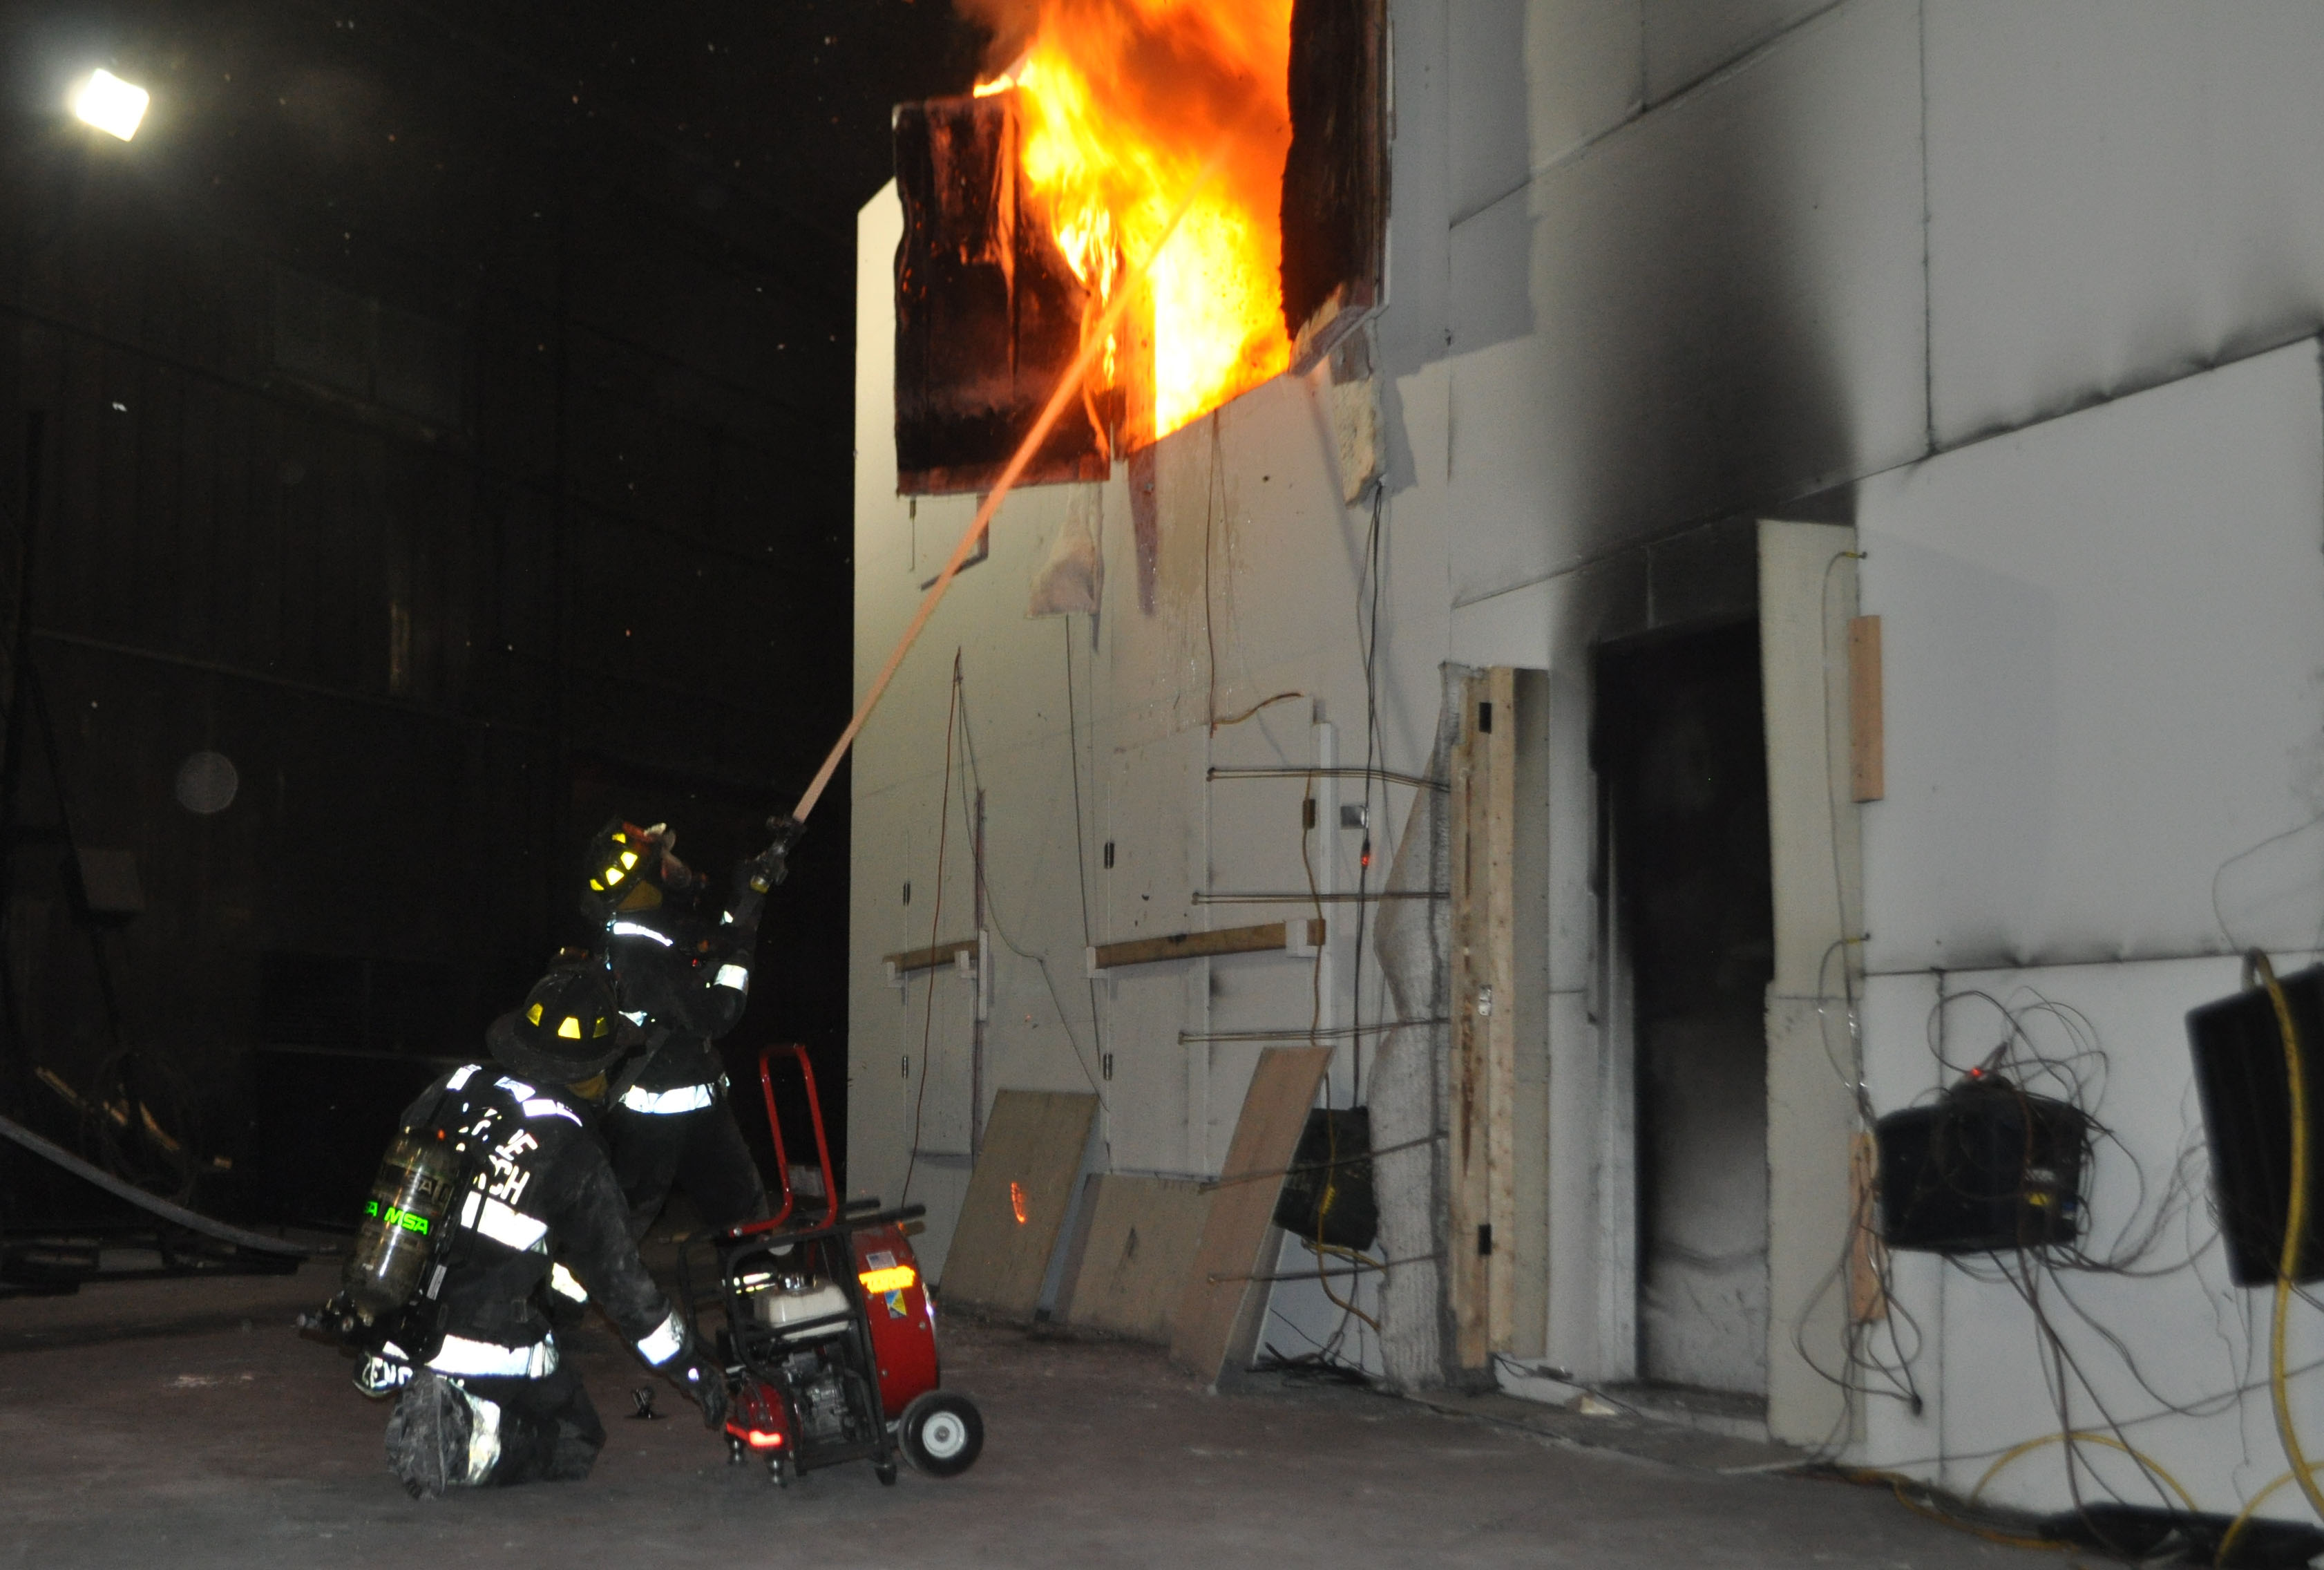
\includegraphics[width=7in]{0_Images/CoverImage.jpg}}}} 

			\vspace*{23\baselineskip} 

		\huge
		\begin{adjustwidth}{-0.5in}{-0in}
		\color{white}
		\textbf{Study of the Effectiveness of Fire Service Positive Pressure Ventilation During Fire Attack in Single Family Homes Incorporating Modern Construction Practices\\}
		\end{adjustwidth}
		\begin{adjustwidth}{-0.5in}{}
		\color{white}
		\vspace{.5in}
		\large
		Stephen Kerber\\
		Director \\
		UL Firefighter Safety Research Institute \\
		\vspace*{\baselineskip}
		Robin Zevotek \\
		Research Engineer \\
		UL Firefighter Safety Research Institue \\ 
		\vspace*{\baselineskip}
		\begin{figure}[h]
			\hspace*{-0.5in}
\includegraphics[width=0.75in]{0_Images/Section_1/ULLogoWhite.pdf}
		\end{figure}
		\end{adjustwidth}
	\end{titlepage}

\renewcommand{\abstractname}{Executive Summary}

\begin{abstract}
There is a continued tragic loss of firefighter and civilian lives, as shown by fire statistics. One significant contributing factor is the lack of understanding of fire behavior in residential structures resulting from the use of ventilation as a firefighter practice on the fire ground. The changing dynamics of residential fires as a result of the changes in home construction materials, contents, size and geometry over the past 30 years compounds our lack of understanding of the effects of ventilation on fire behavior.  Positive Pressure Ventilation (PPV) fans were introduced as a technology to increase firefighter safety by controlling the ventilation.  However, adequate scientific data is not available for PPV to be used without increasing the risk to firefighters.

This fire research project will develop experimental data from full-scale house fire experiments to examine positive pressure ventilation used during fire attack, suppression techniques and the resulting fire behavior. The experimental results will be used to develop tactical considerations outlining firefighting ventilation and suppression practices that will reduce firefighter death and injury.  This fire research project will draw from and enhance previous DHS AFG sponsored research (EMW-2008-FP-01774) which studied the impact of horizontal ventilation through doors and windows and (EMW-2010-FP-00661) which studied the impact of vertical ventilation through the roof. This project will address the concerns the firefighter community has expressed and provide a baseline for choosing the most appropriate type or types of ventilation on the fire ground.  Upon completion, the fire service will have scientific based comparisons between the three types of ventilation used on the fireground everyday across the country.  A comprehensive fire service outreach program will make sure that this science meets the street.
\end{abstract}

\newpage

\section*{Introduction}
NFPA estimates that from 2002-2011, U.S. fire departments responded to an average of 398,000 residential fires annually. \cite{NFFF} These fires caused an estimated annual average of 2,820 civilian deaths and 13,780 civilian injuries. More than 70\% of the reported home fires and 84\% of the fatal home fire injuries occurred in one- or two- family dwellings, with the remainder in apartments or similar properties. For the 2006-2009 period, there were an estimated annual average 35,743 firefighter fire ground injuries in the U.S. The rate of traumatic firefighter deaths occurring outside structures or from cardiac arrest has declined, while at the same time, firefighter deaths occurring inside structures has continued to climb over the past 30 years.4 Ventilation is believed to be a significant contributing factor to this continued climb in firefighter injuries and deaths.  Developing the proper knowledge about the use of PPV would enable more departments to implement its use with the confidence of knowing when to apply it to increase the safety of their members, whether in place of or supplementing current ventilation tactics.

\section{Background}

\section{Objectives and Technical Plan}

\section{Project Technical Panel}

\section{Previous Literature}
\subsection{Fire Service Publications}
\subsection{Fire Service Training Manuals}
\subsection{Firefighter Line of Duty Deaths}
\subsection{Research Work}

\section{Instrumentation}

\section{Test Set Up}
\subsection{Structures}
\subsection{Fuel Load}
\paragraph{Furniture Description} \mbox{}

Furniture was acquired for the experiments such that each room of furniture was the same from experiment to experiment. Descriptions, dimensions and weights for all of the furniture used are in Table \ref{FurnitureTable}. Images of each piece of furniture can be seen in Figure \ref{fig:FurnitureImages}.

\renewcommand{\arraystretch}{1.5}
\begin{table}[H]
	\centering
	\caption{Furniture Dimensions and Weight}
		\begin{tabular}[c]{|c|c|c|c|c|}
			\hline
			\textbf{Item} & \textbf{Length (in.)} & \textbf{Width (in.)} & \textbf{Height (in.)} & \textbf{Weight (lbs.)} \\ \hline \hline
			Kitchen Table & 30 & 30 & 30 & 45.2 \\ \hline
			Kitchen Table Chair & 17.5 & 19 & 33 & 15.5 \\ \hline
			Night Stand & 27 & 17 & 23.5 & 59.3 \\ \hline
			Full Box Spring & 79 & 52.5 & 9 & 42.1 \\ \hline
			Mattress & 80 & 53 & 8 & 53 \\ \hline
			Comforter & 92 & 104 & - & - \\ \hline
			Standard Pillow & 24 & 16 & 3 & 1.5 \\ \hline
			Flat Sheet & 98 & 83 & - & 3.5 \\ \hline
			Headboard & 54 & 18 & 2.5 & 34.1 \\ \hline
			Dresser & 44.5 & 24 & 35.5 & 212.6 \\ \hline
			Foot Stool & 23 & 18 & 16.5 & 16.1 \\ \hline
			Round End Table & 24 & 24 & 22 & 32.3 \\ \hline
			Coffee Table & 30 & 18 & 18 & 25 \\ \hline
			Lamp \& Shade & 12 & 12 & 22 & 6.3 \\ \hline
			Chair (Yellow) & 30 & 30.5 & 34 & 34.8 \\ \hline
			Chair (Brown) & 32 & 32 & 33 & 82.1 \\ \hline
			Sleeper Sofa (Green) & 84 & 36.5 & 33 & 208 \\ \hline
			Sleeper Sofa (Orange) & 65 &35.5 & 31.5 & 145.1 \\ \hline
			Curtain & - & 225 & 100 & 18 \\ \hline	
			Base Kitchen Cabinet & 36 & 24 & 34.5 & 70.7 \\ \hline
			Wall Kitchen Cabinet & 25 & 12 & 30 & 34.6 \\ \hline
		\end{tabular}
	\label{FurnitureTable}
\end{table}

\begin{figure}
	\centering
	\begin{tabular}[c]{c c c c}
		\subfloat[Kitchen Table]{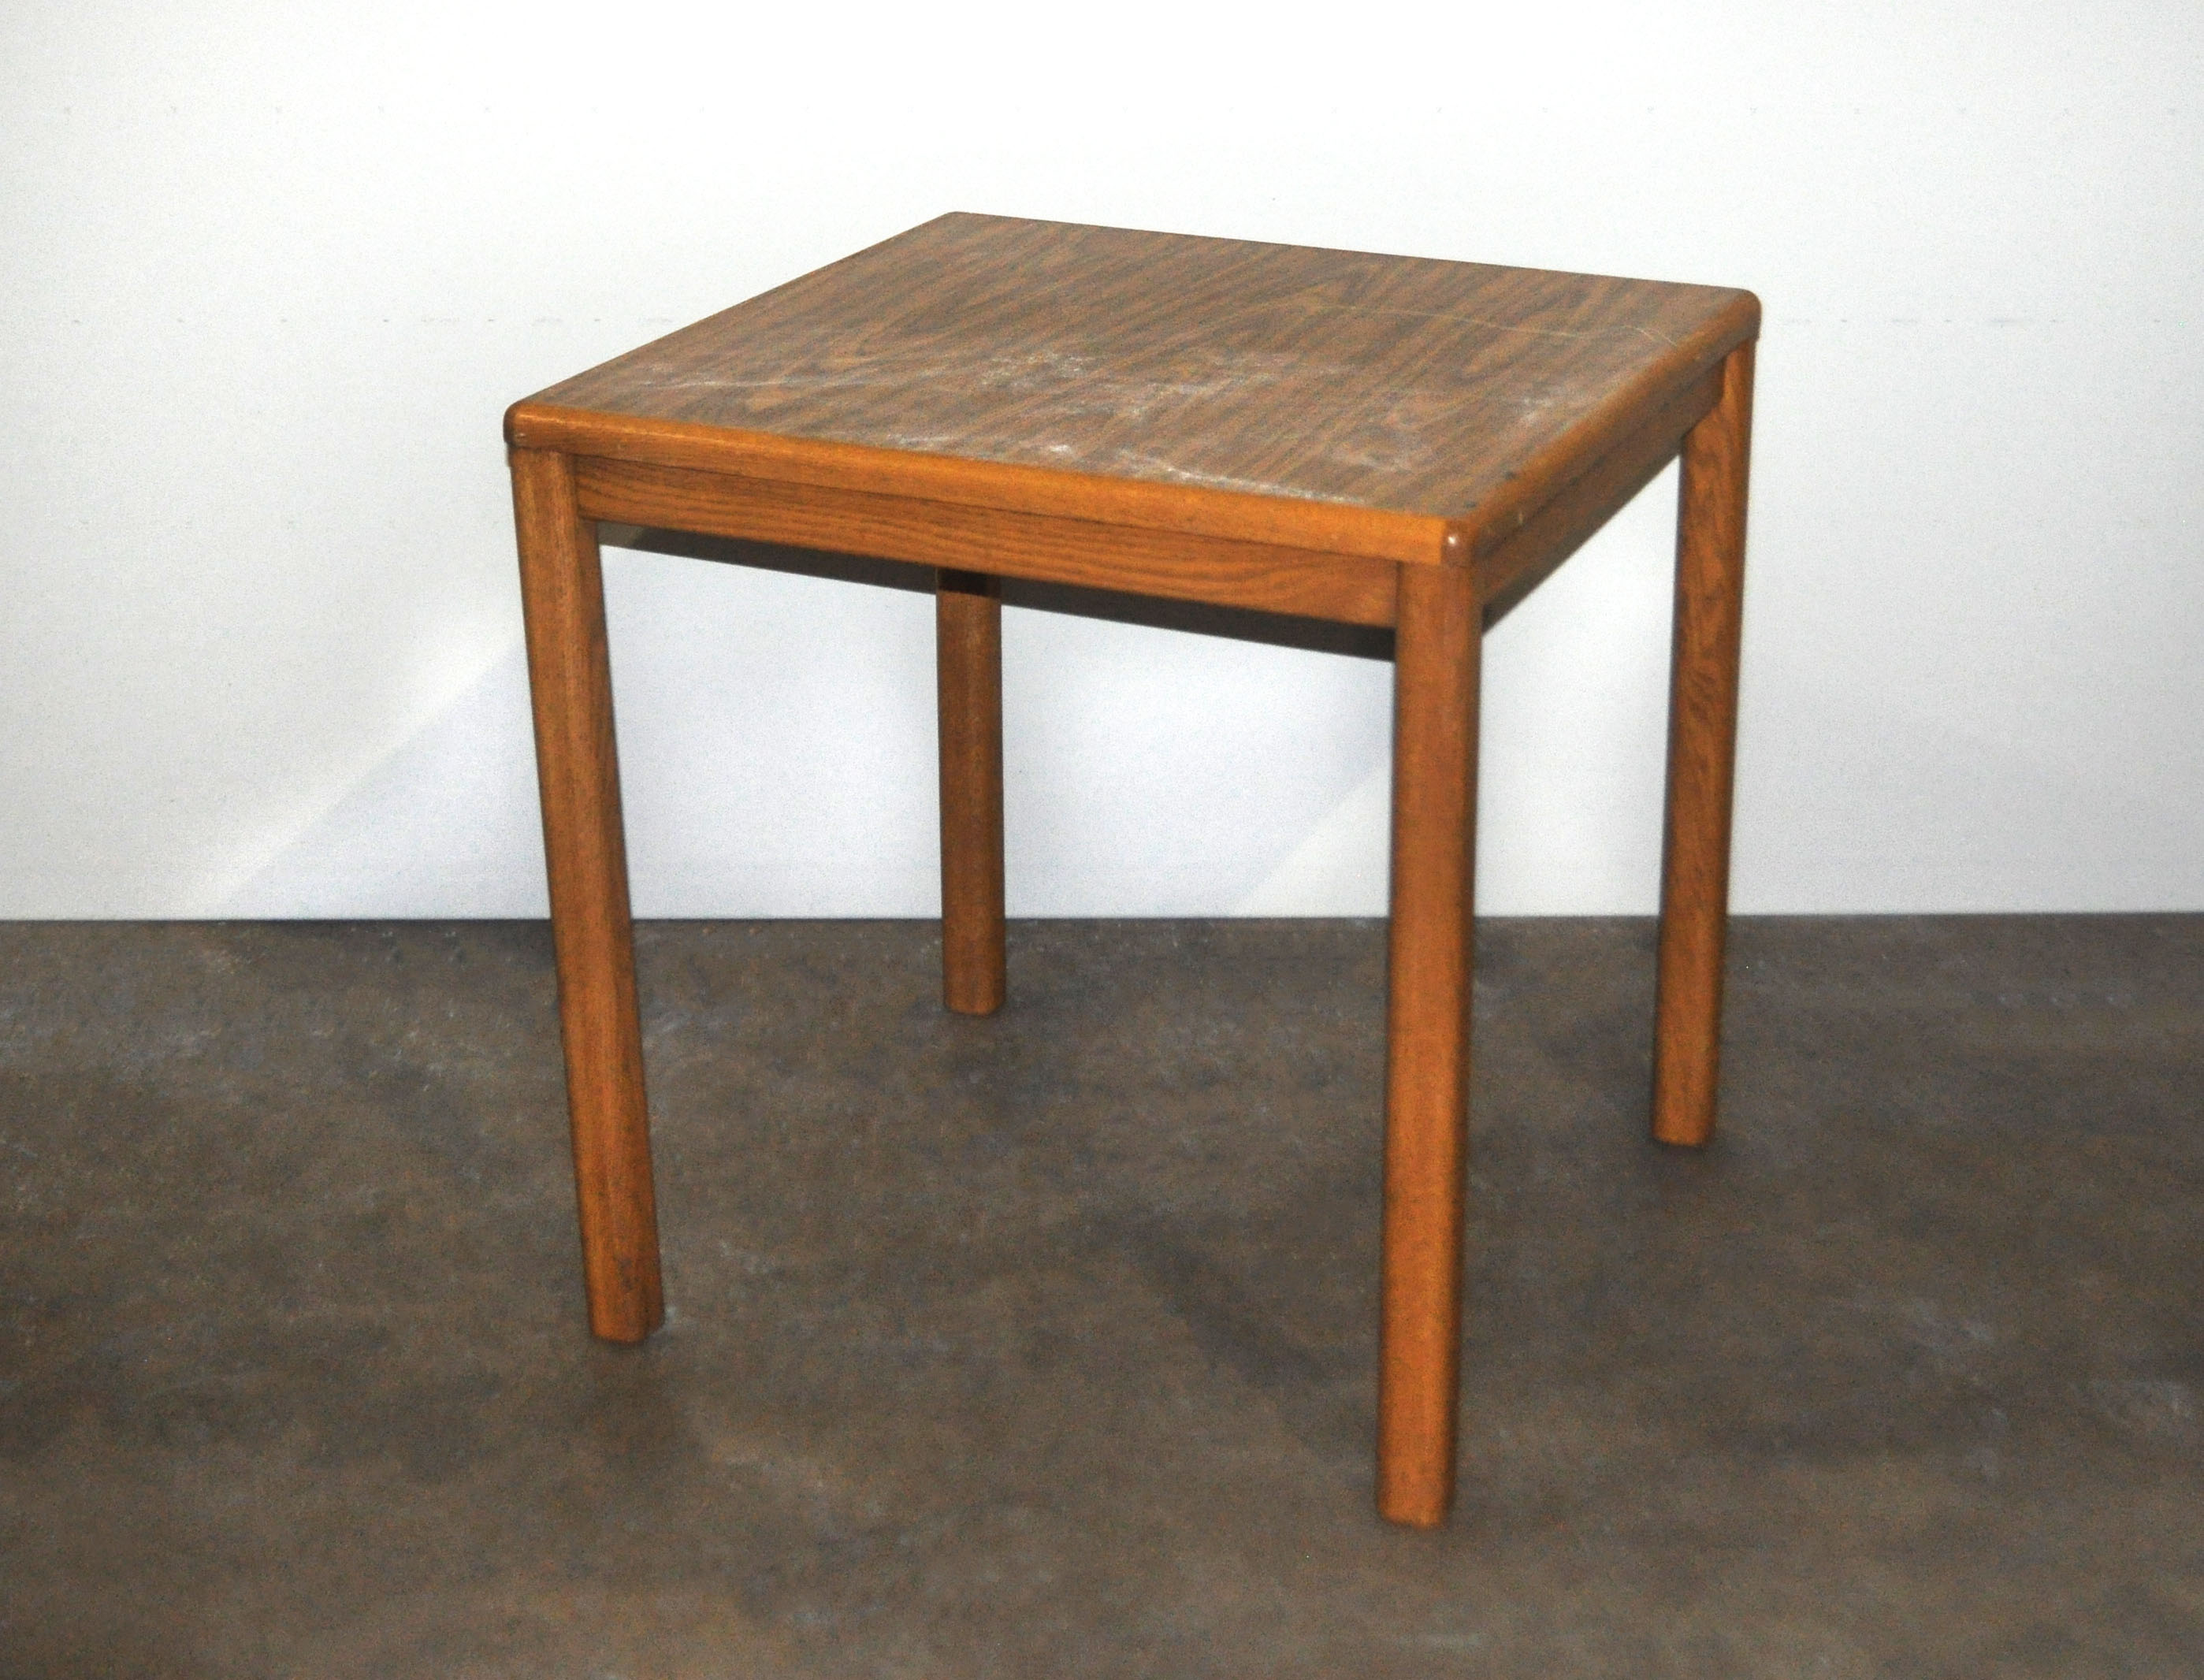
\includegraphics[width=3cm]{0_Images/Furniture/KitchenTable.jpg}} &
		\subfloat[Kitchen Chair]{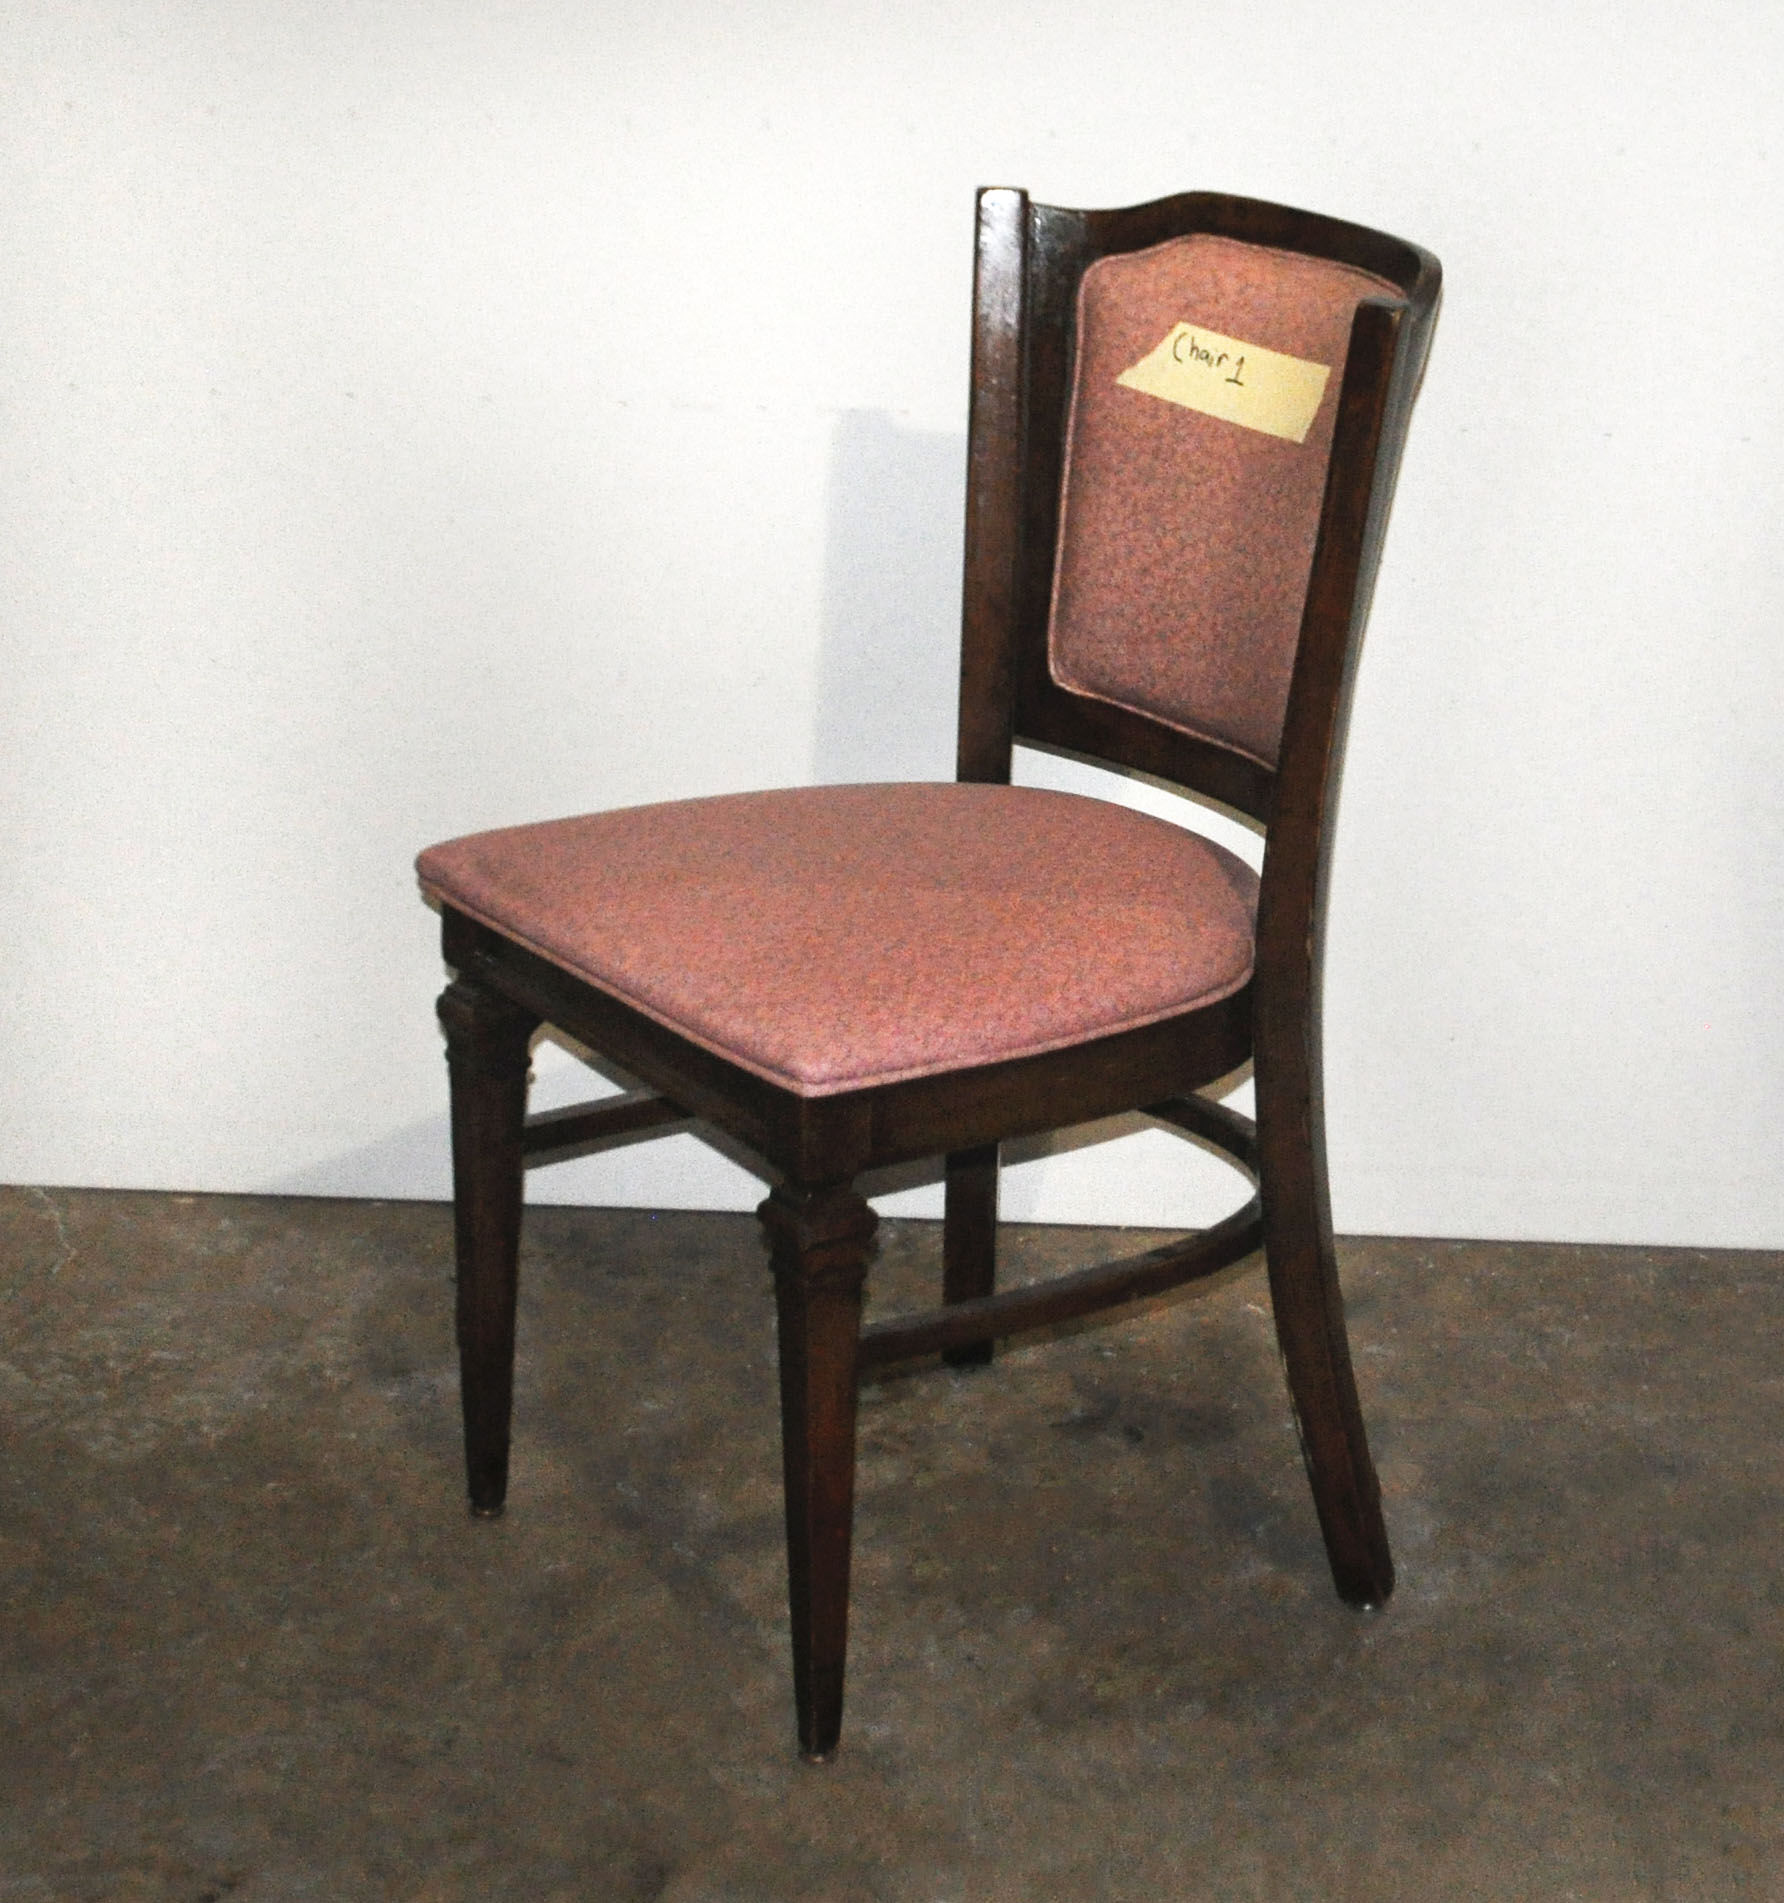
\includegraphics[width=3cm]{0_Images/Furniture/KitchenTableChair.jpg}} &
		\subfloat[Night Stand]{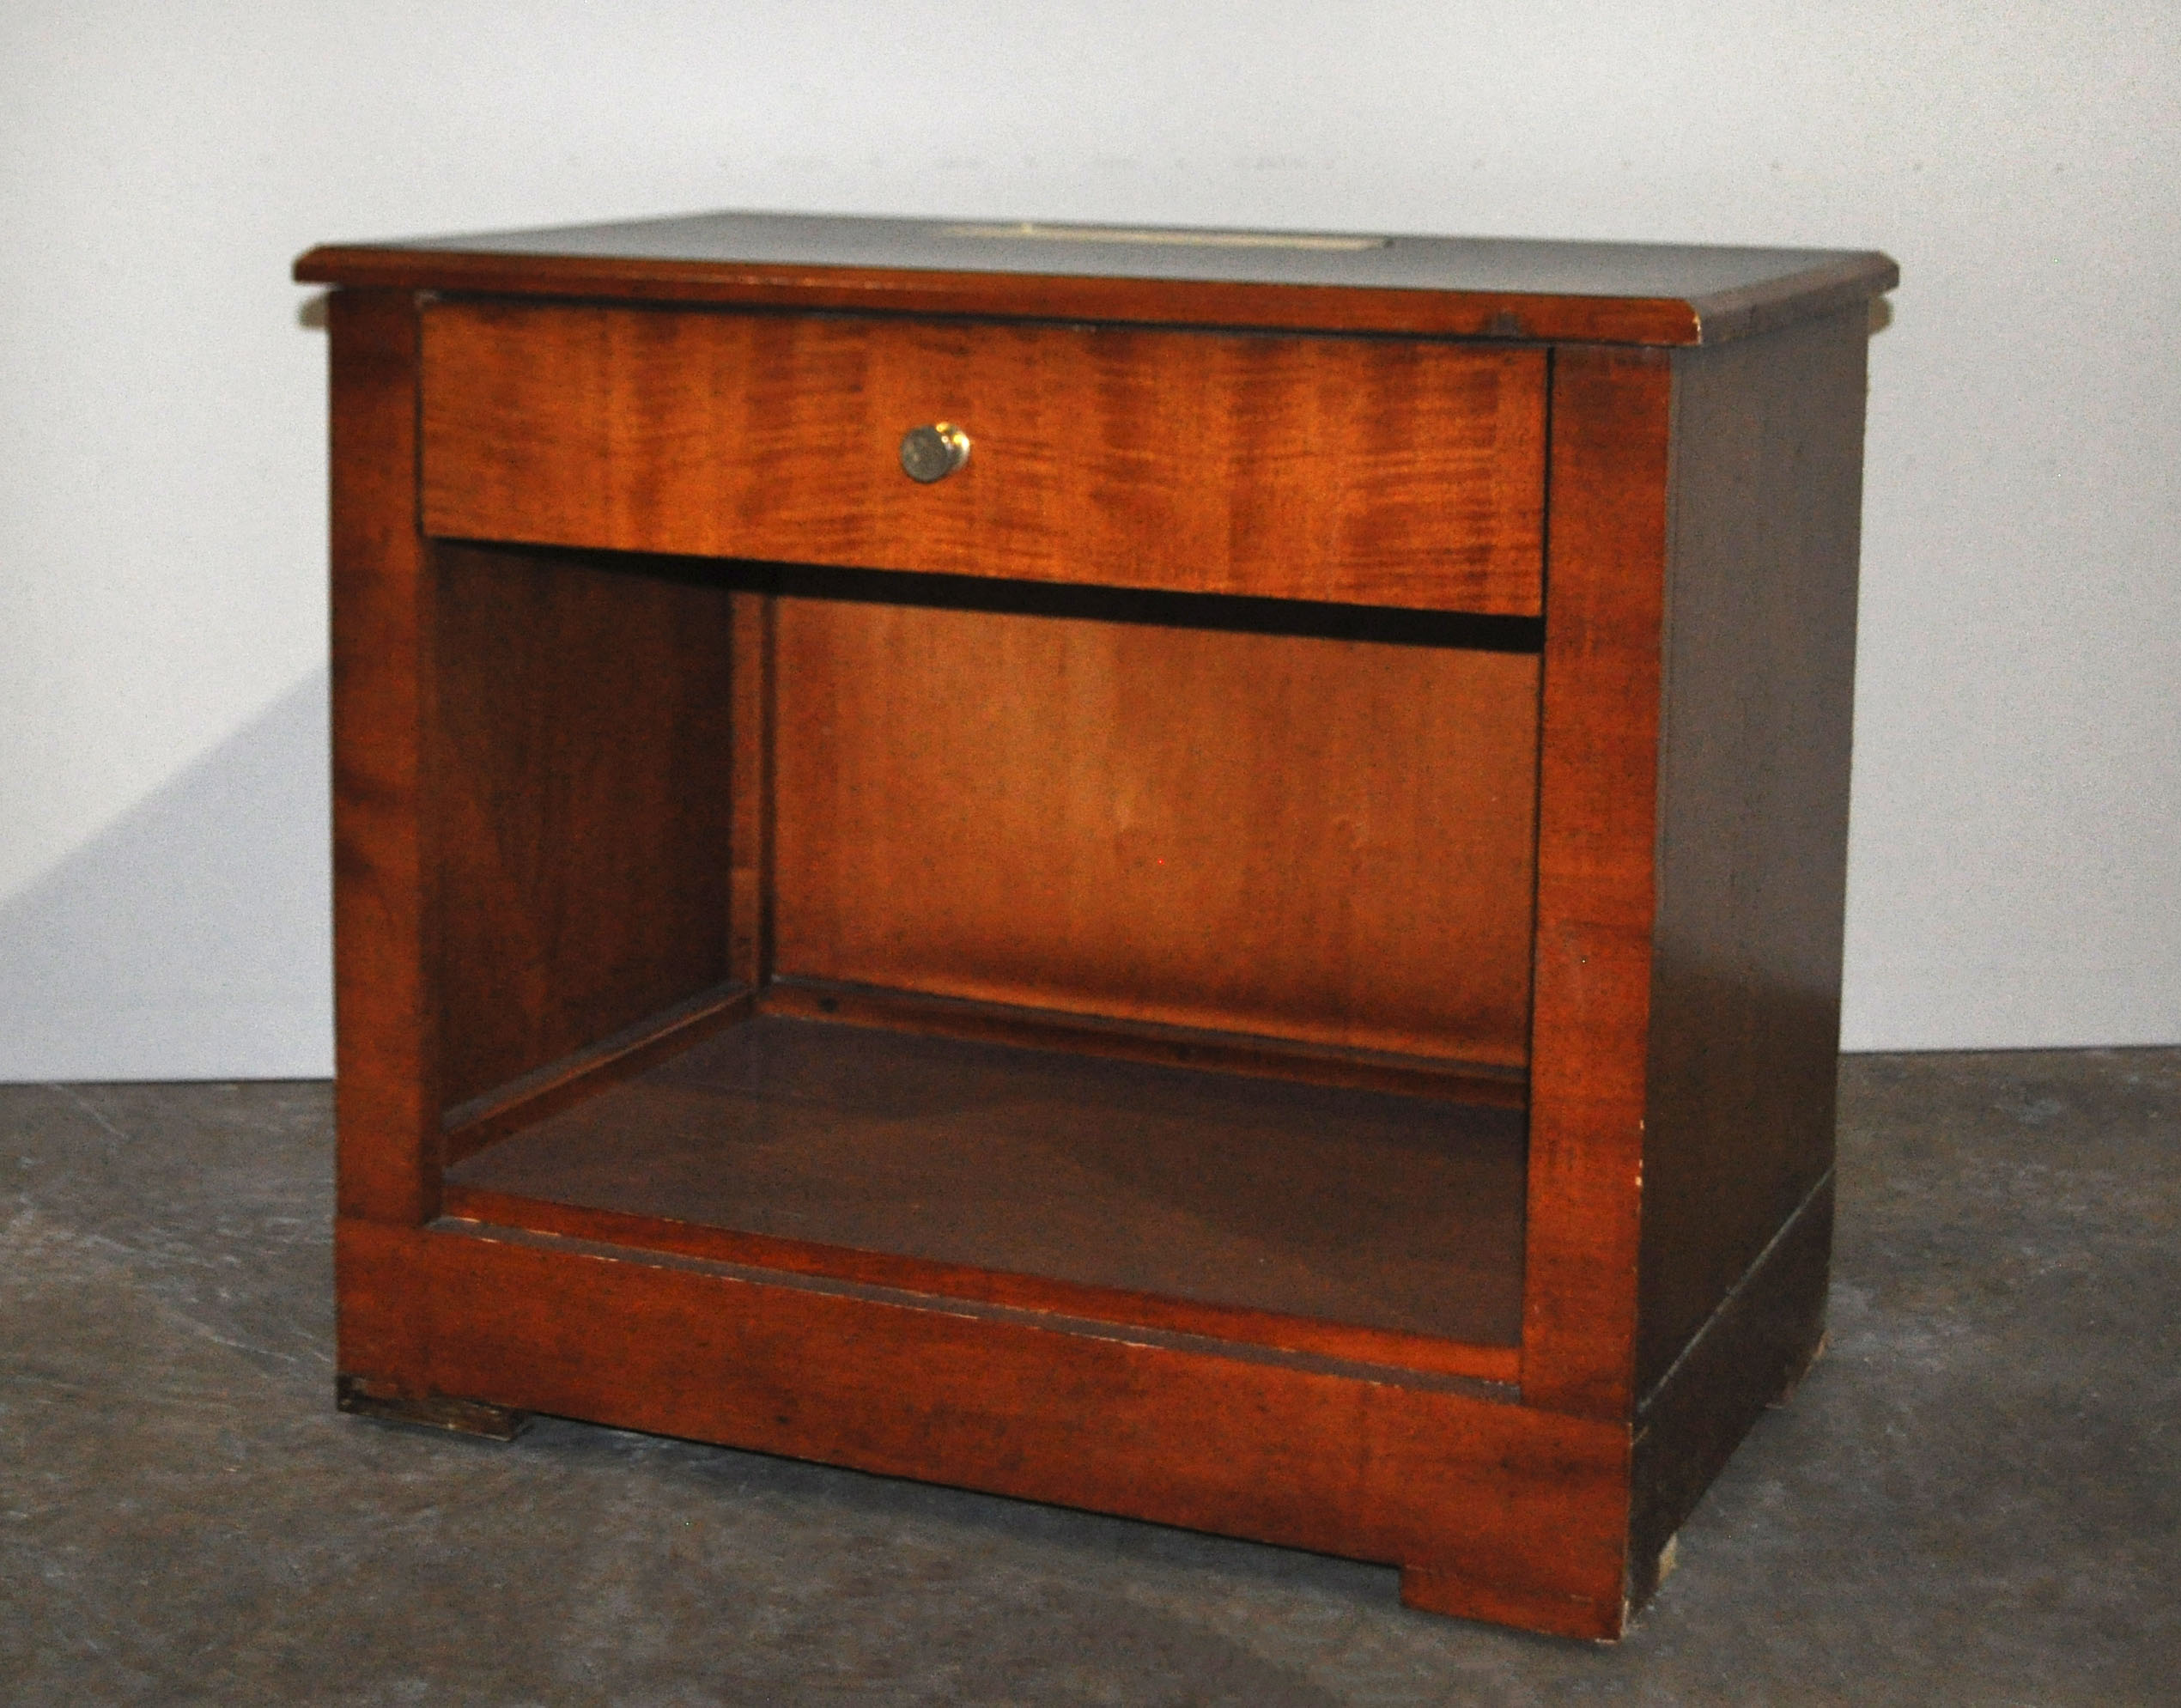
\includegraphics[width=3cm]{0_Images/Furniture/NightStand.jpg}} &
		\subfloat[Box Spring]{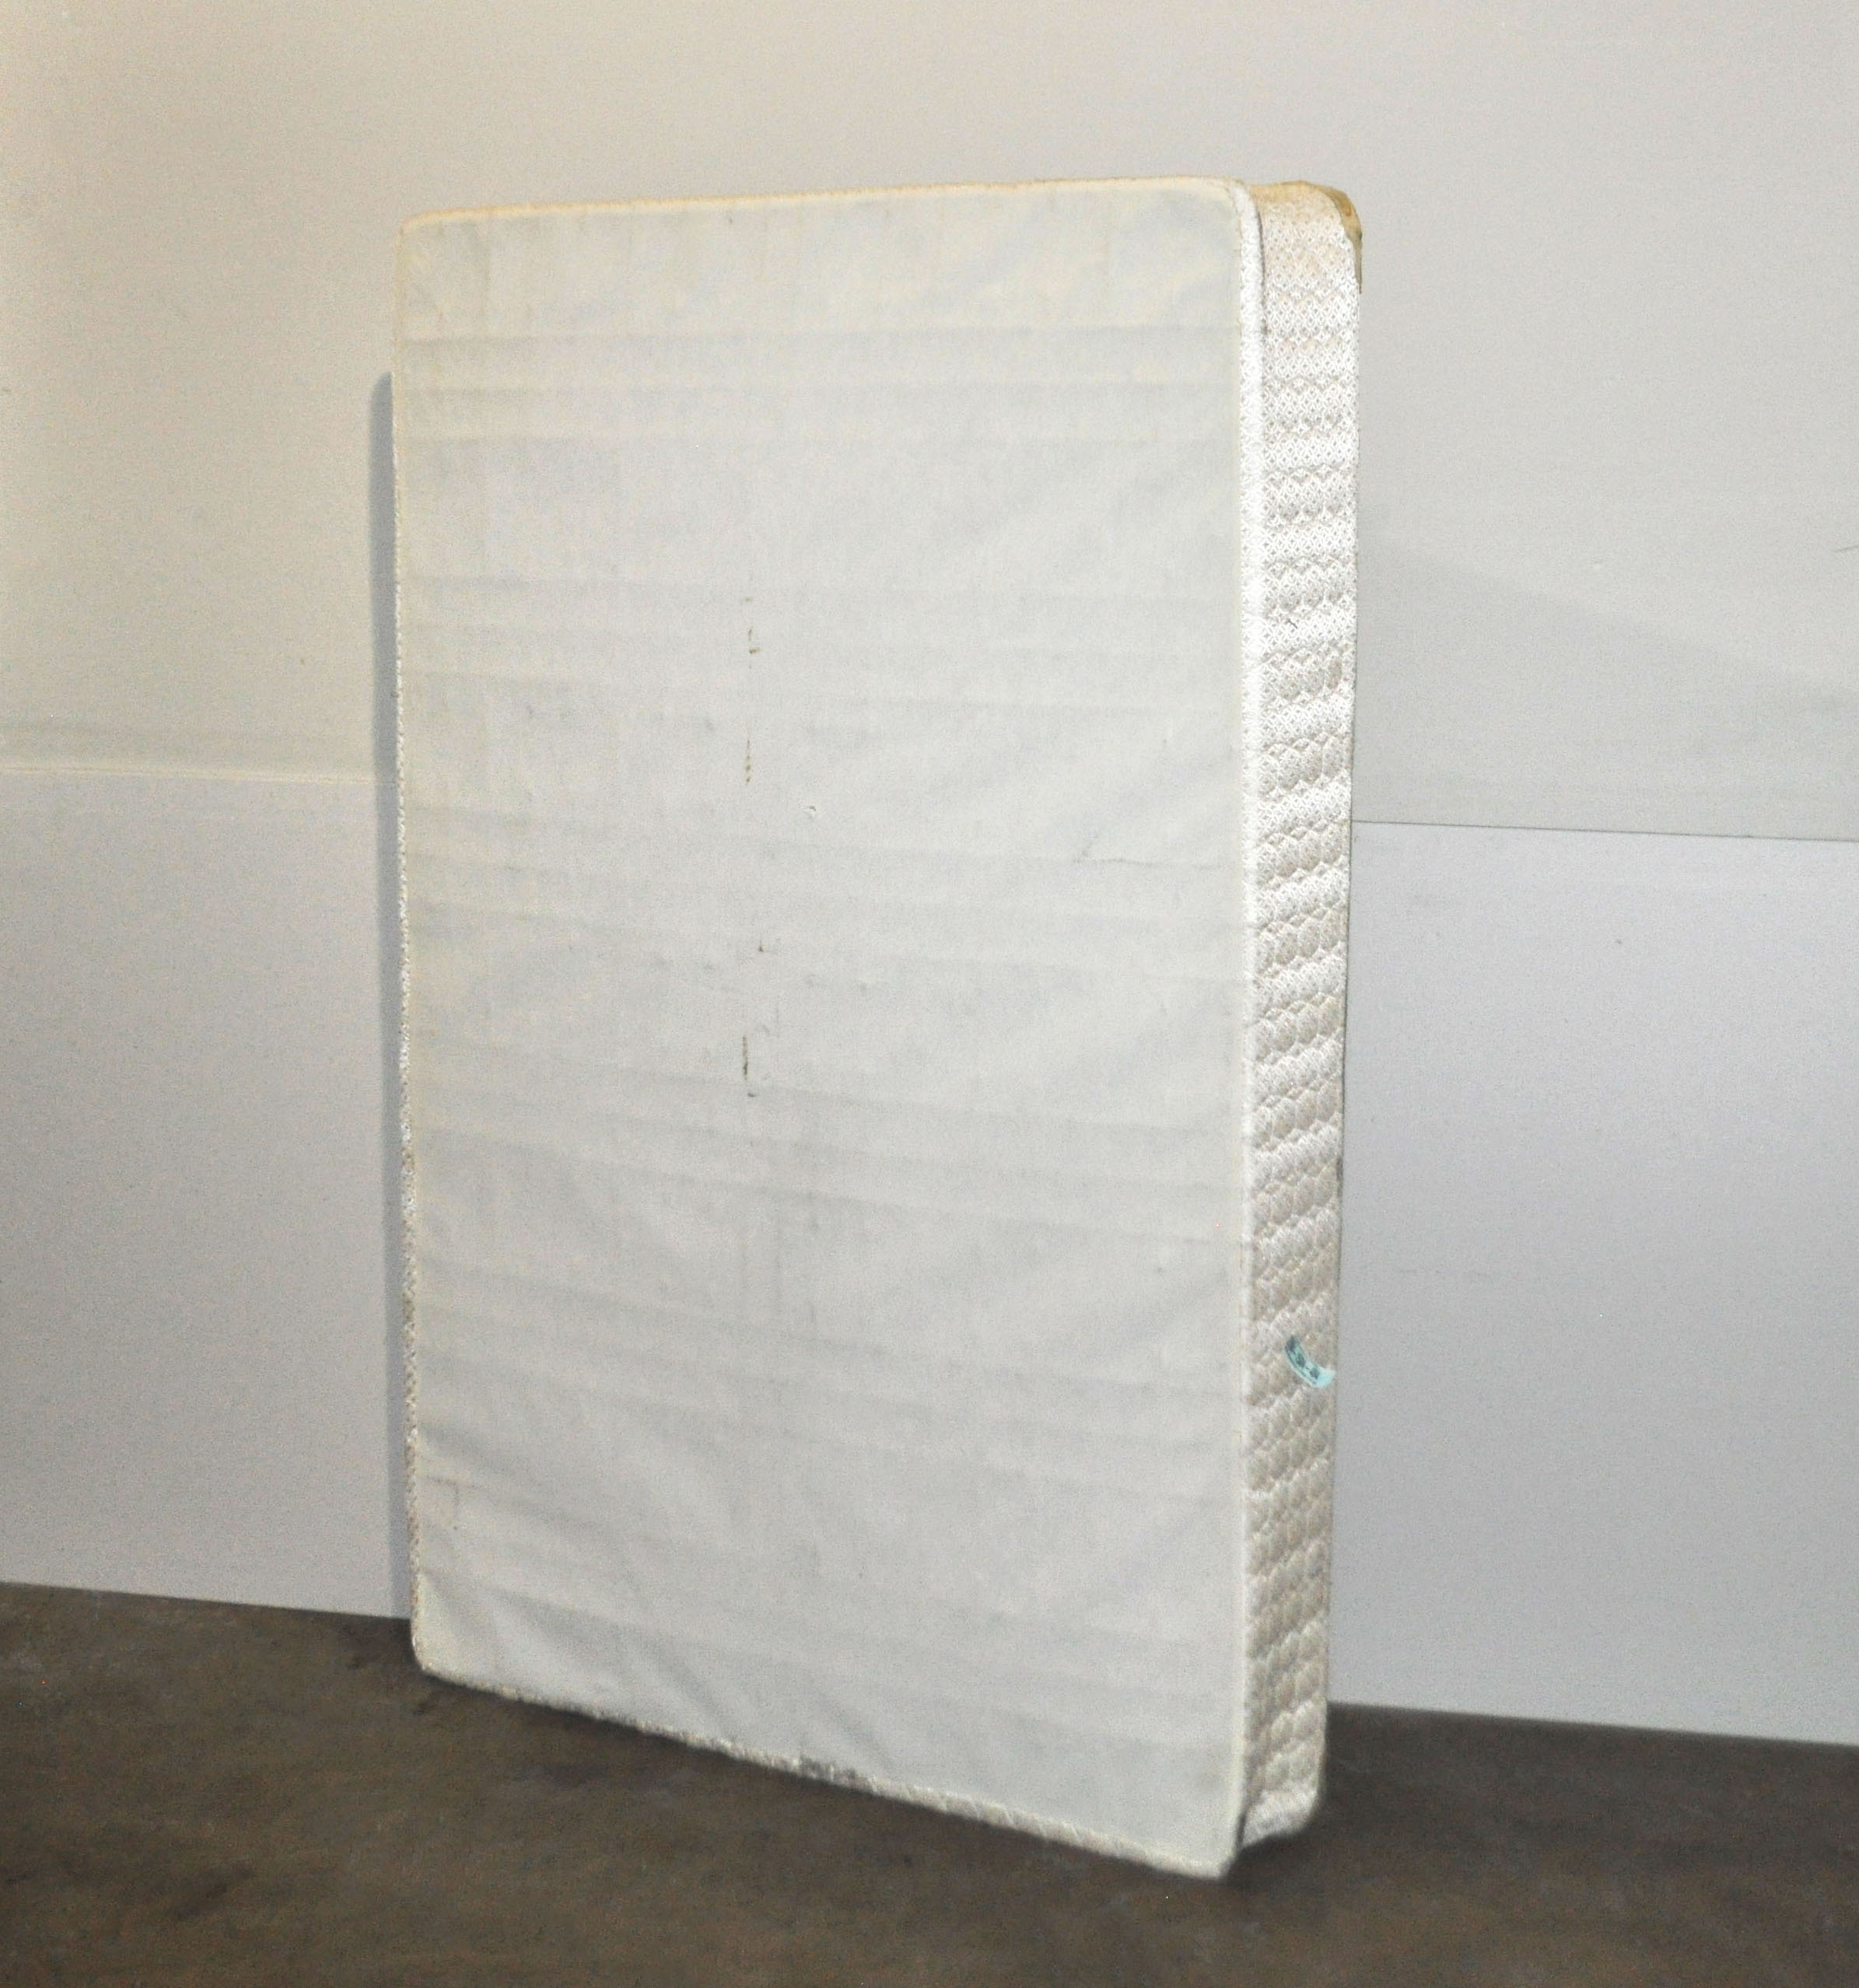
\includegraphics[width=3cm]{0_Images/Furniture/BoxSpring.jpg}} \\
		\subfloat[Matress]{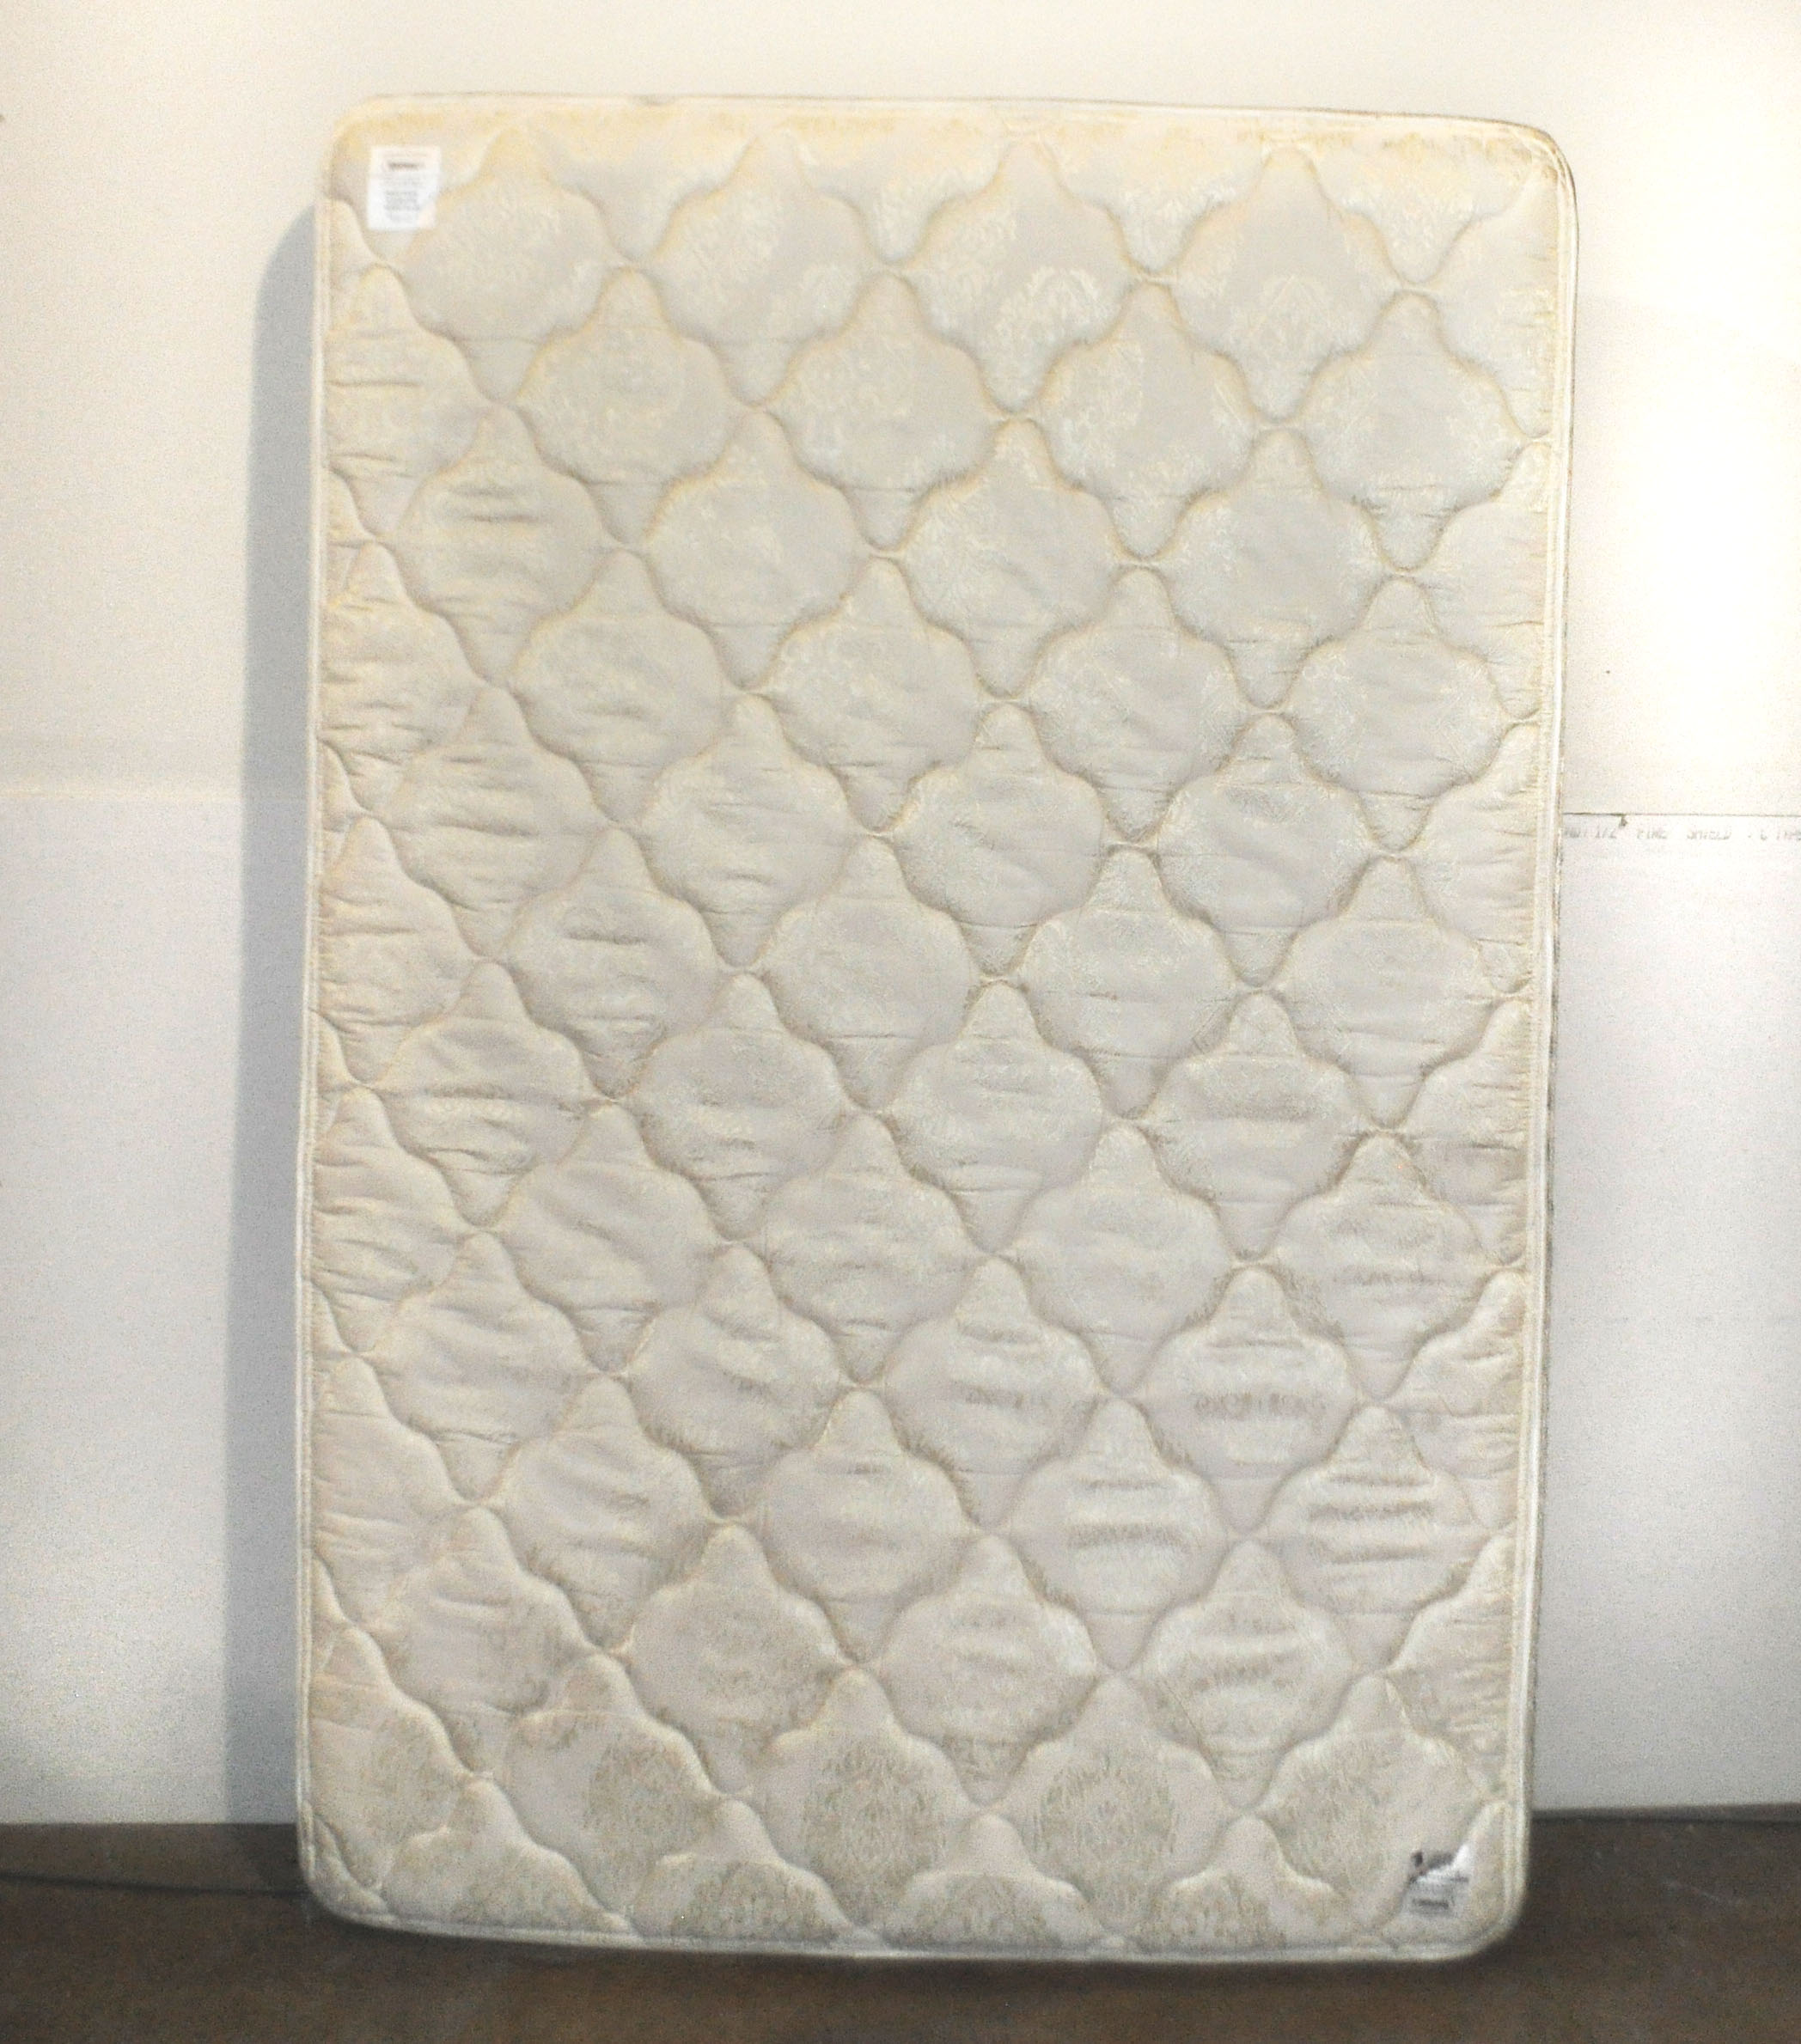
\includegraphics[width=3cm]{0_Images/Furniture/Matress.jpg}} &
		\subfloat[Head Board]{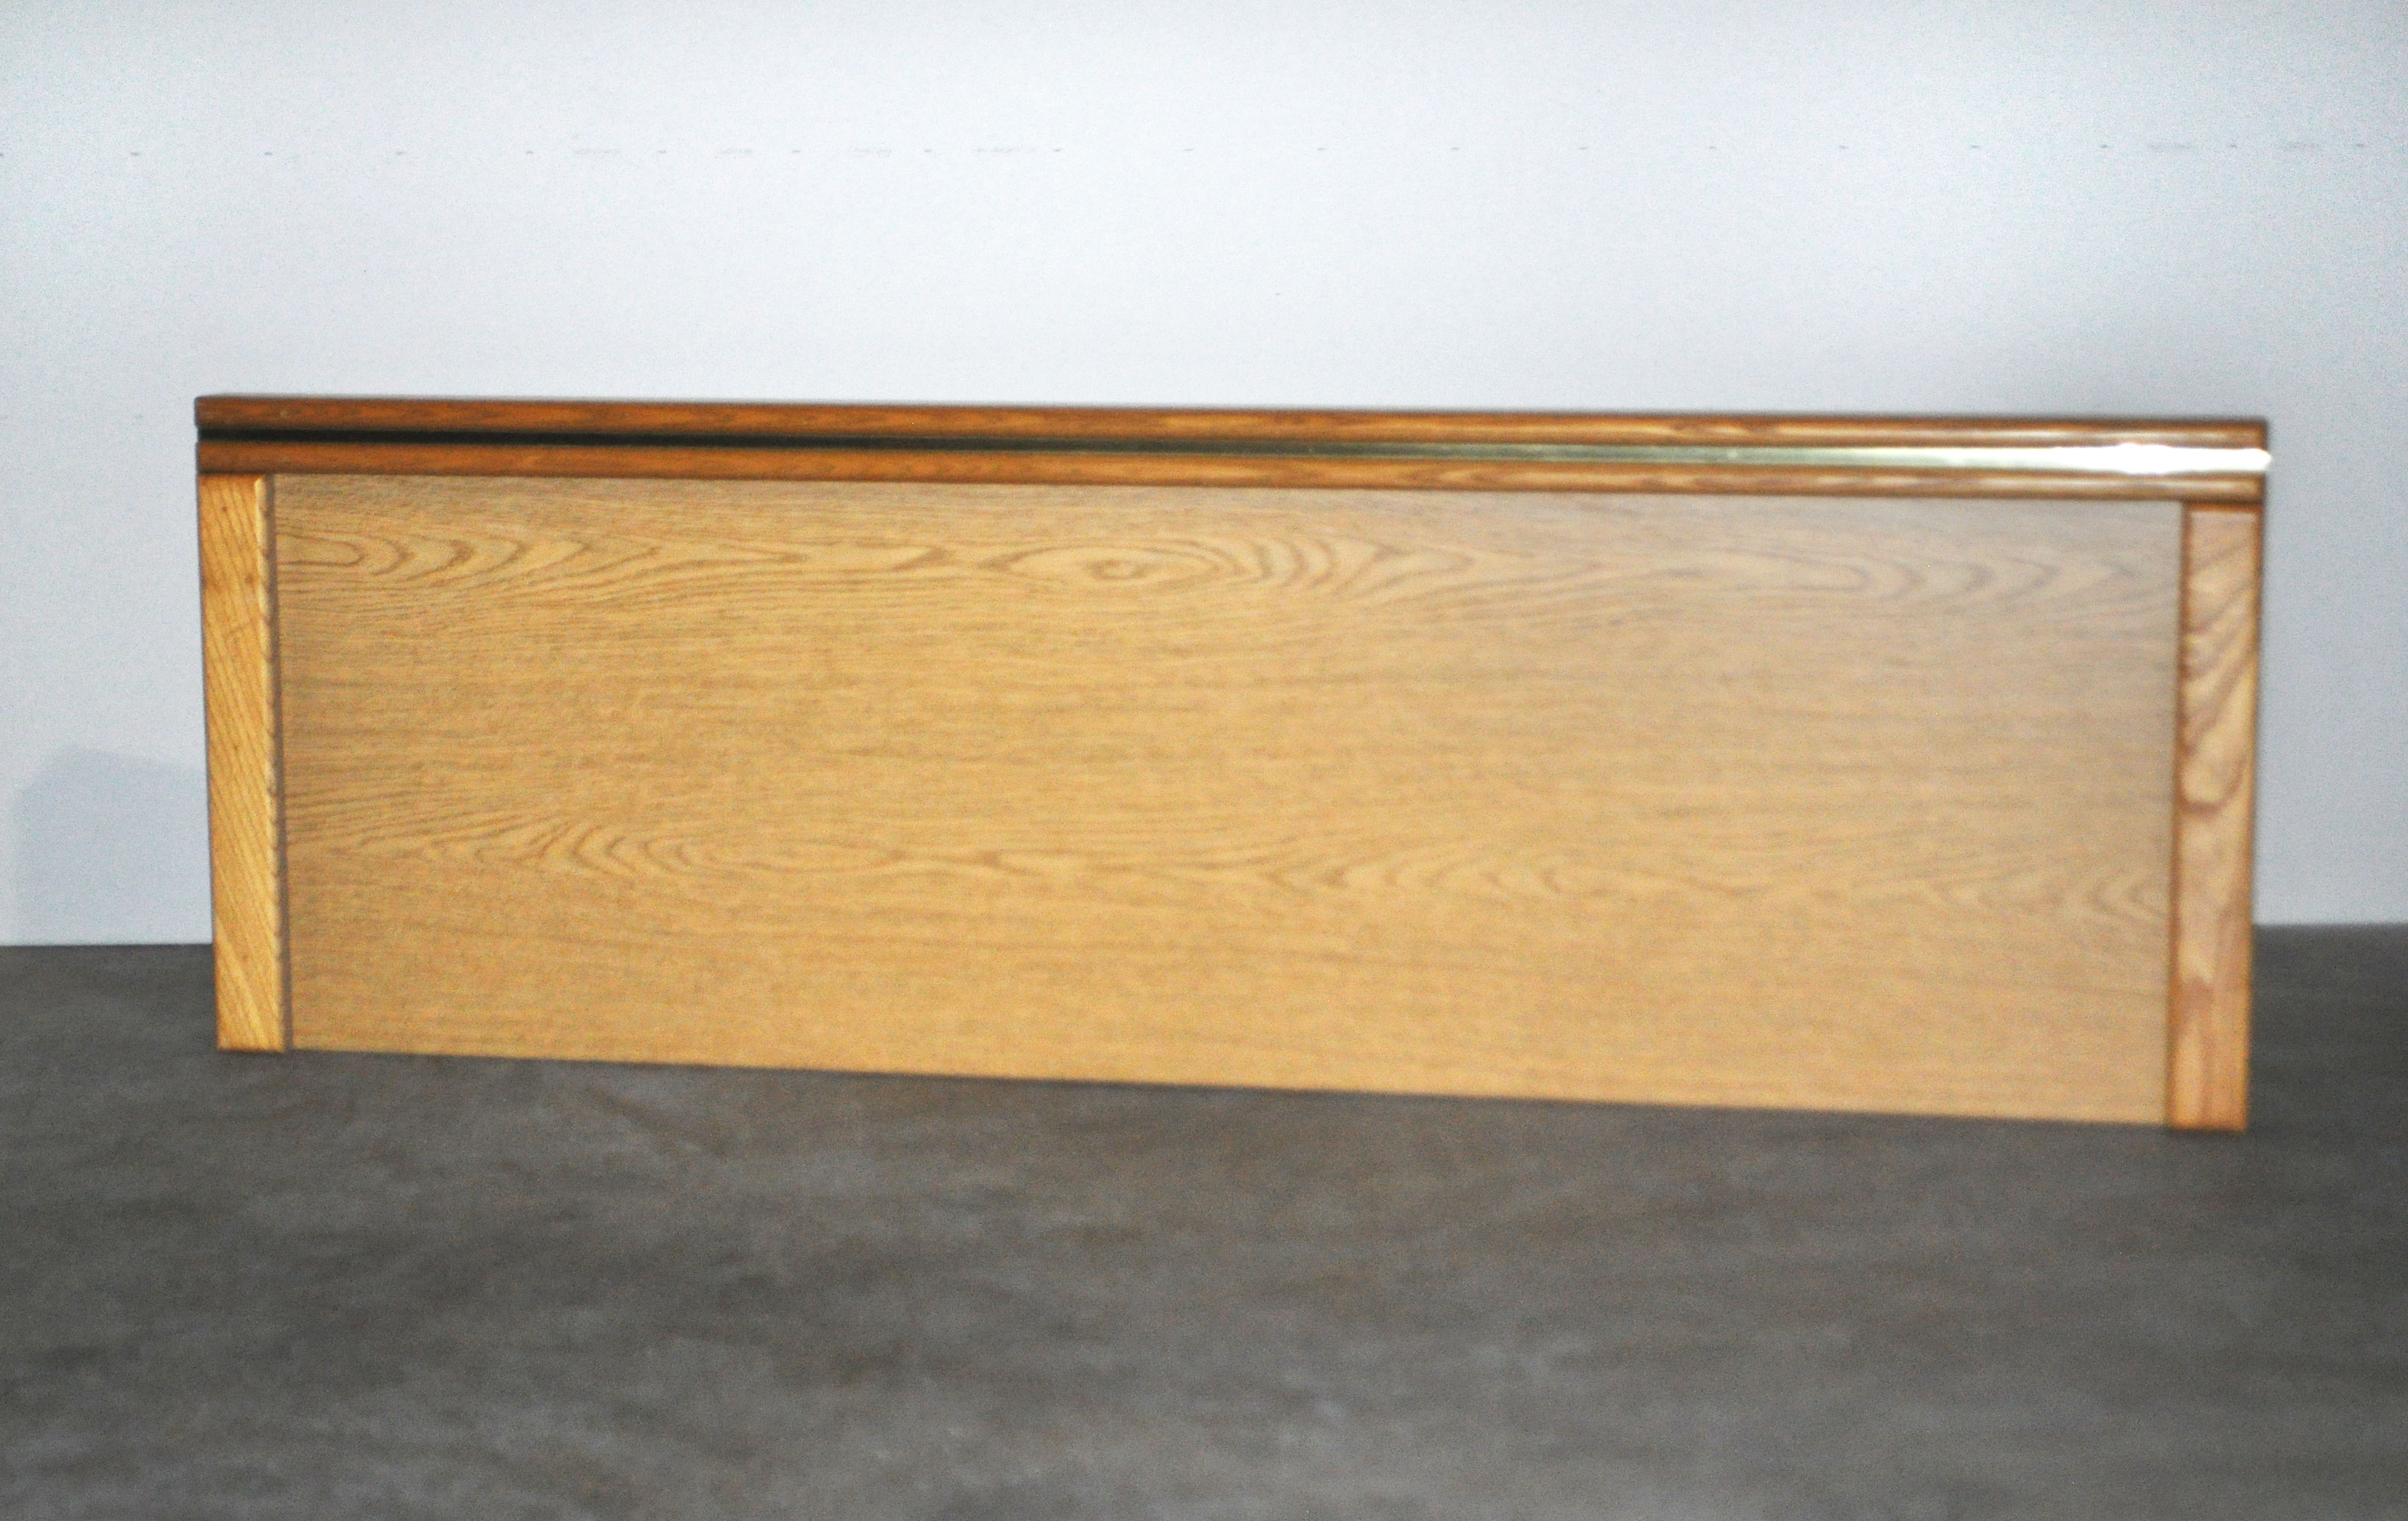
\includegraphics[width=3cm]{0_Images/Furniture/HeadBoard.jpg}} &
		\subfloat[Dresser]{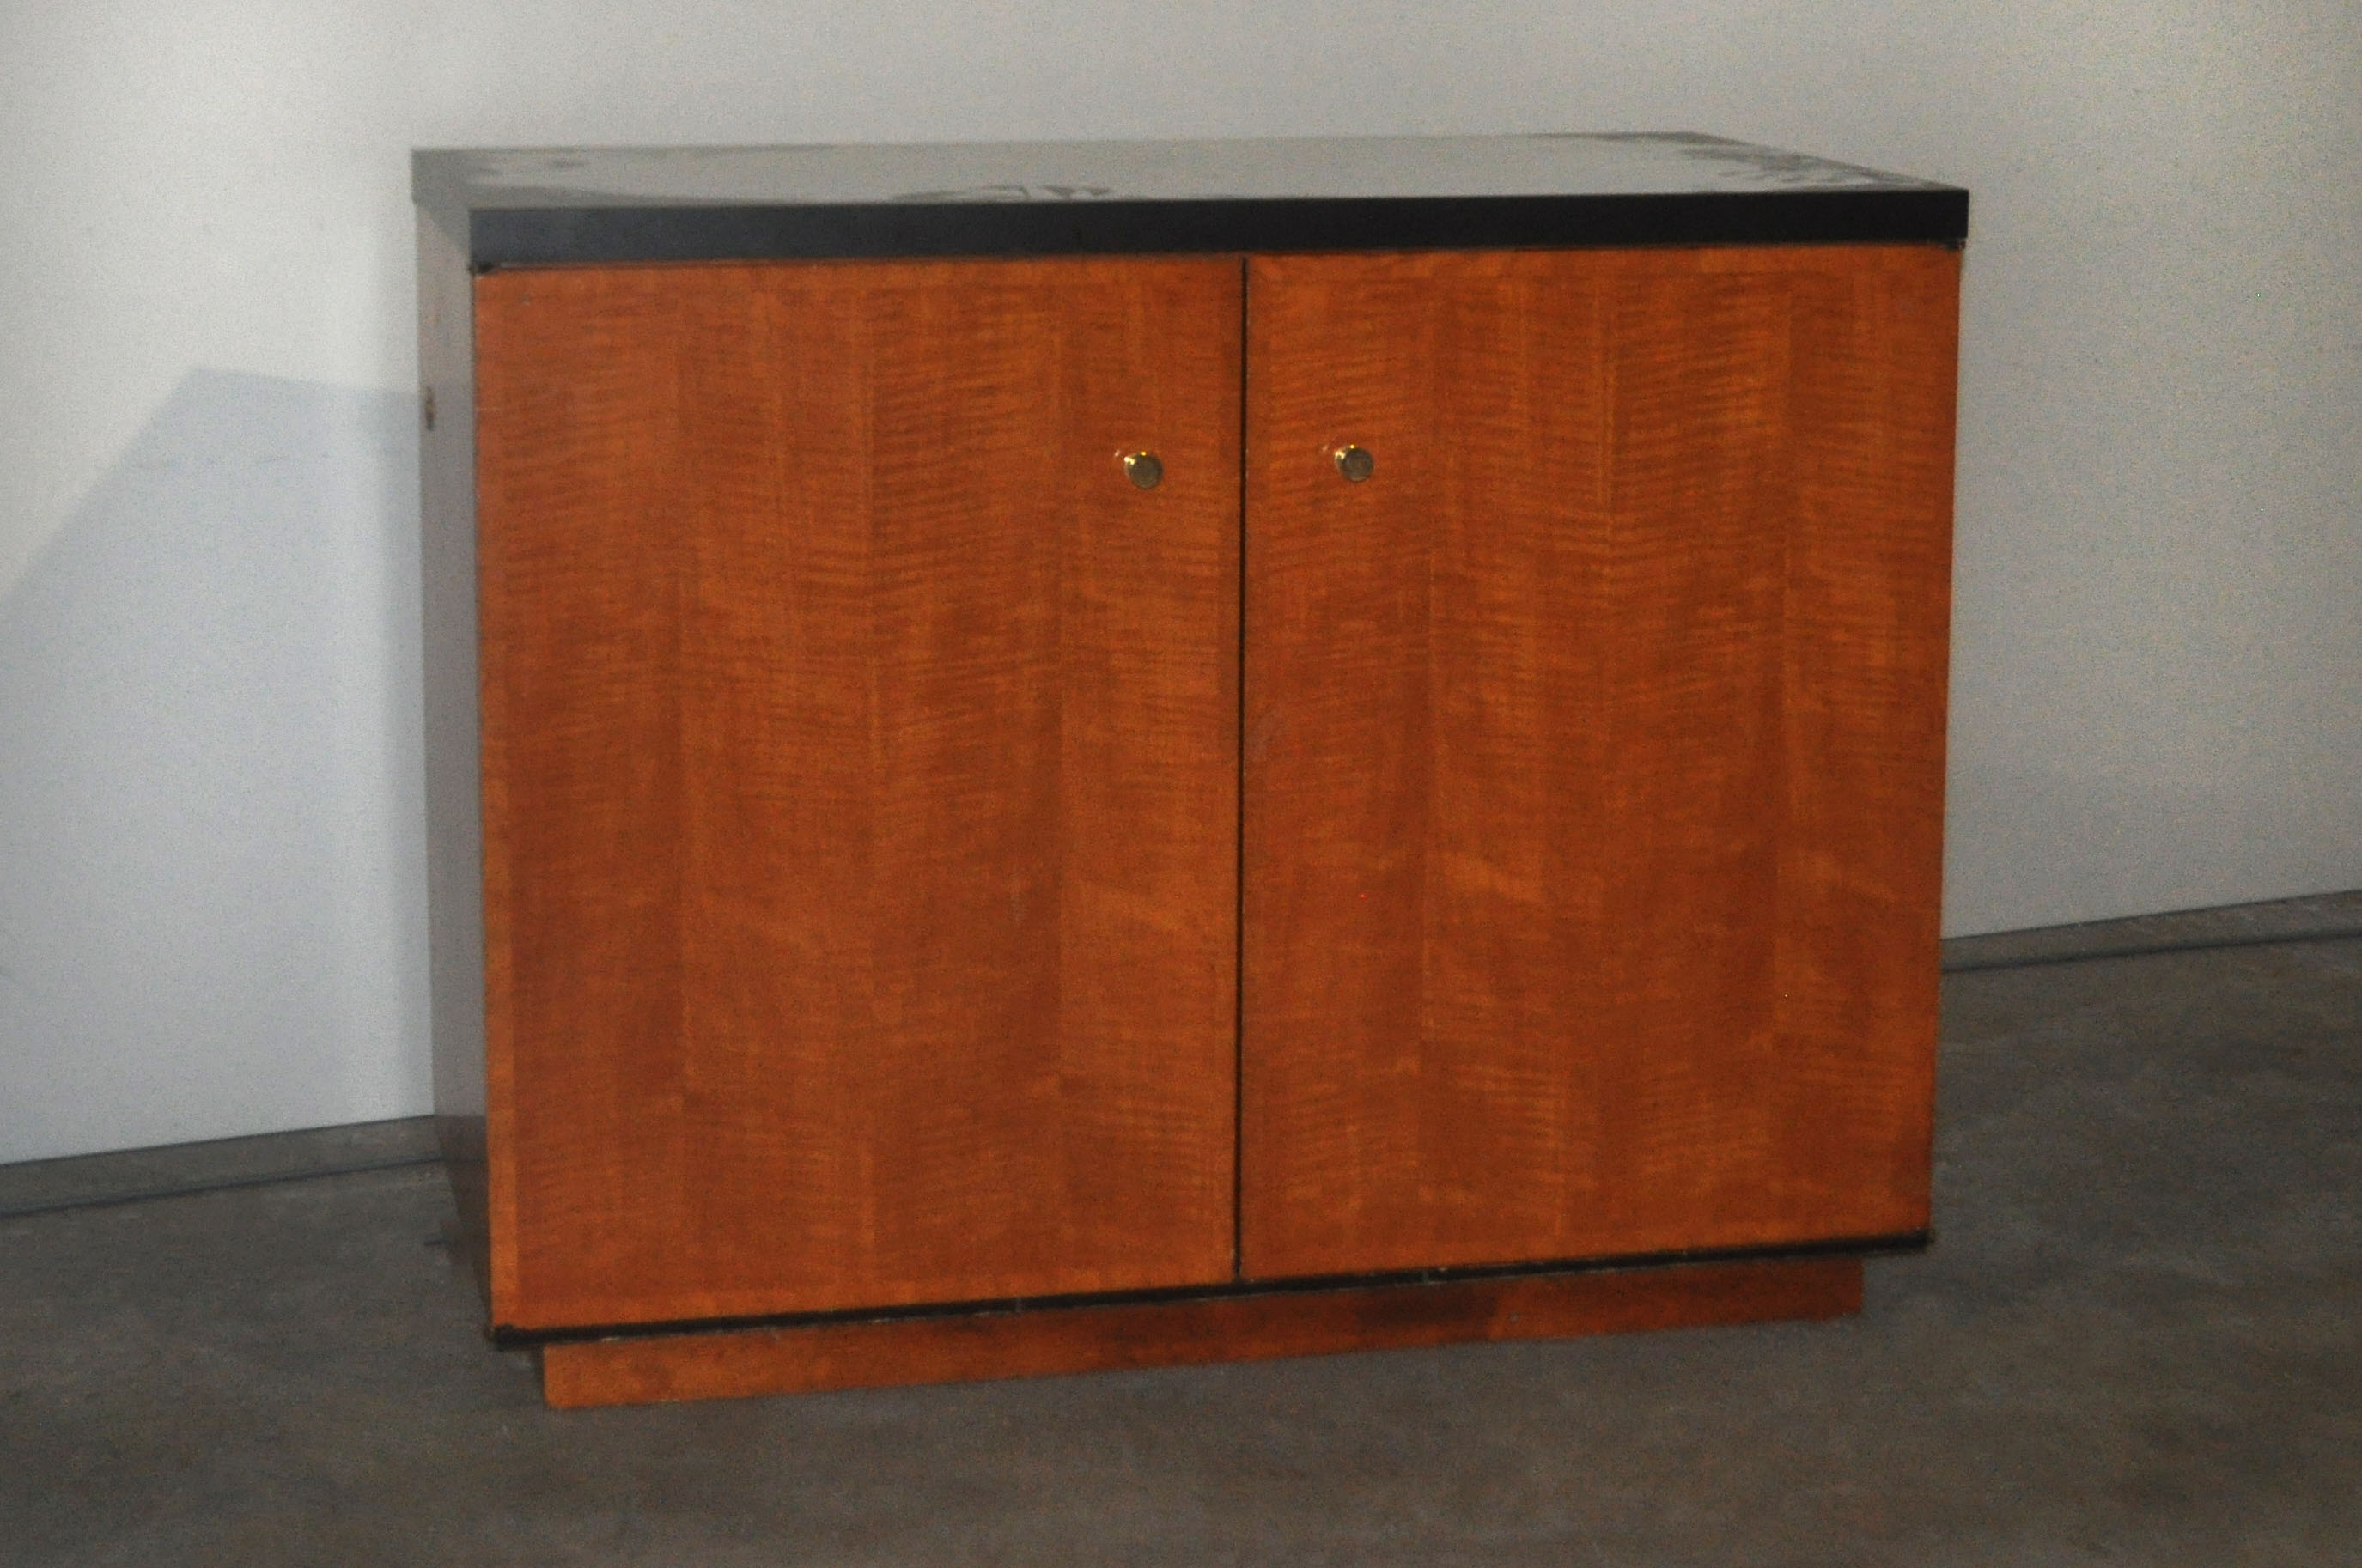
\includegraphics[width=3cm]{0_Images/Furniture/Dresser_TVStand.jpg}} &
		\subfloat[Foot Stool]{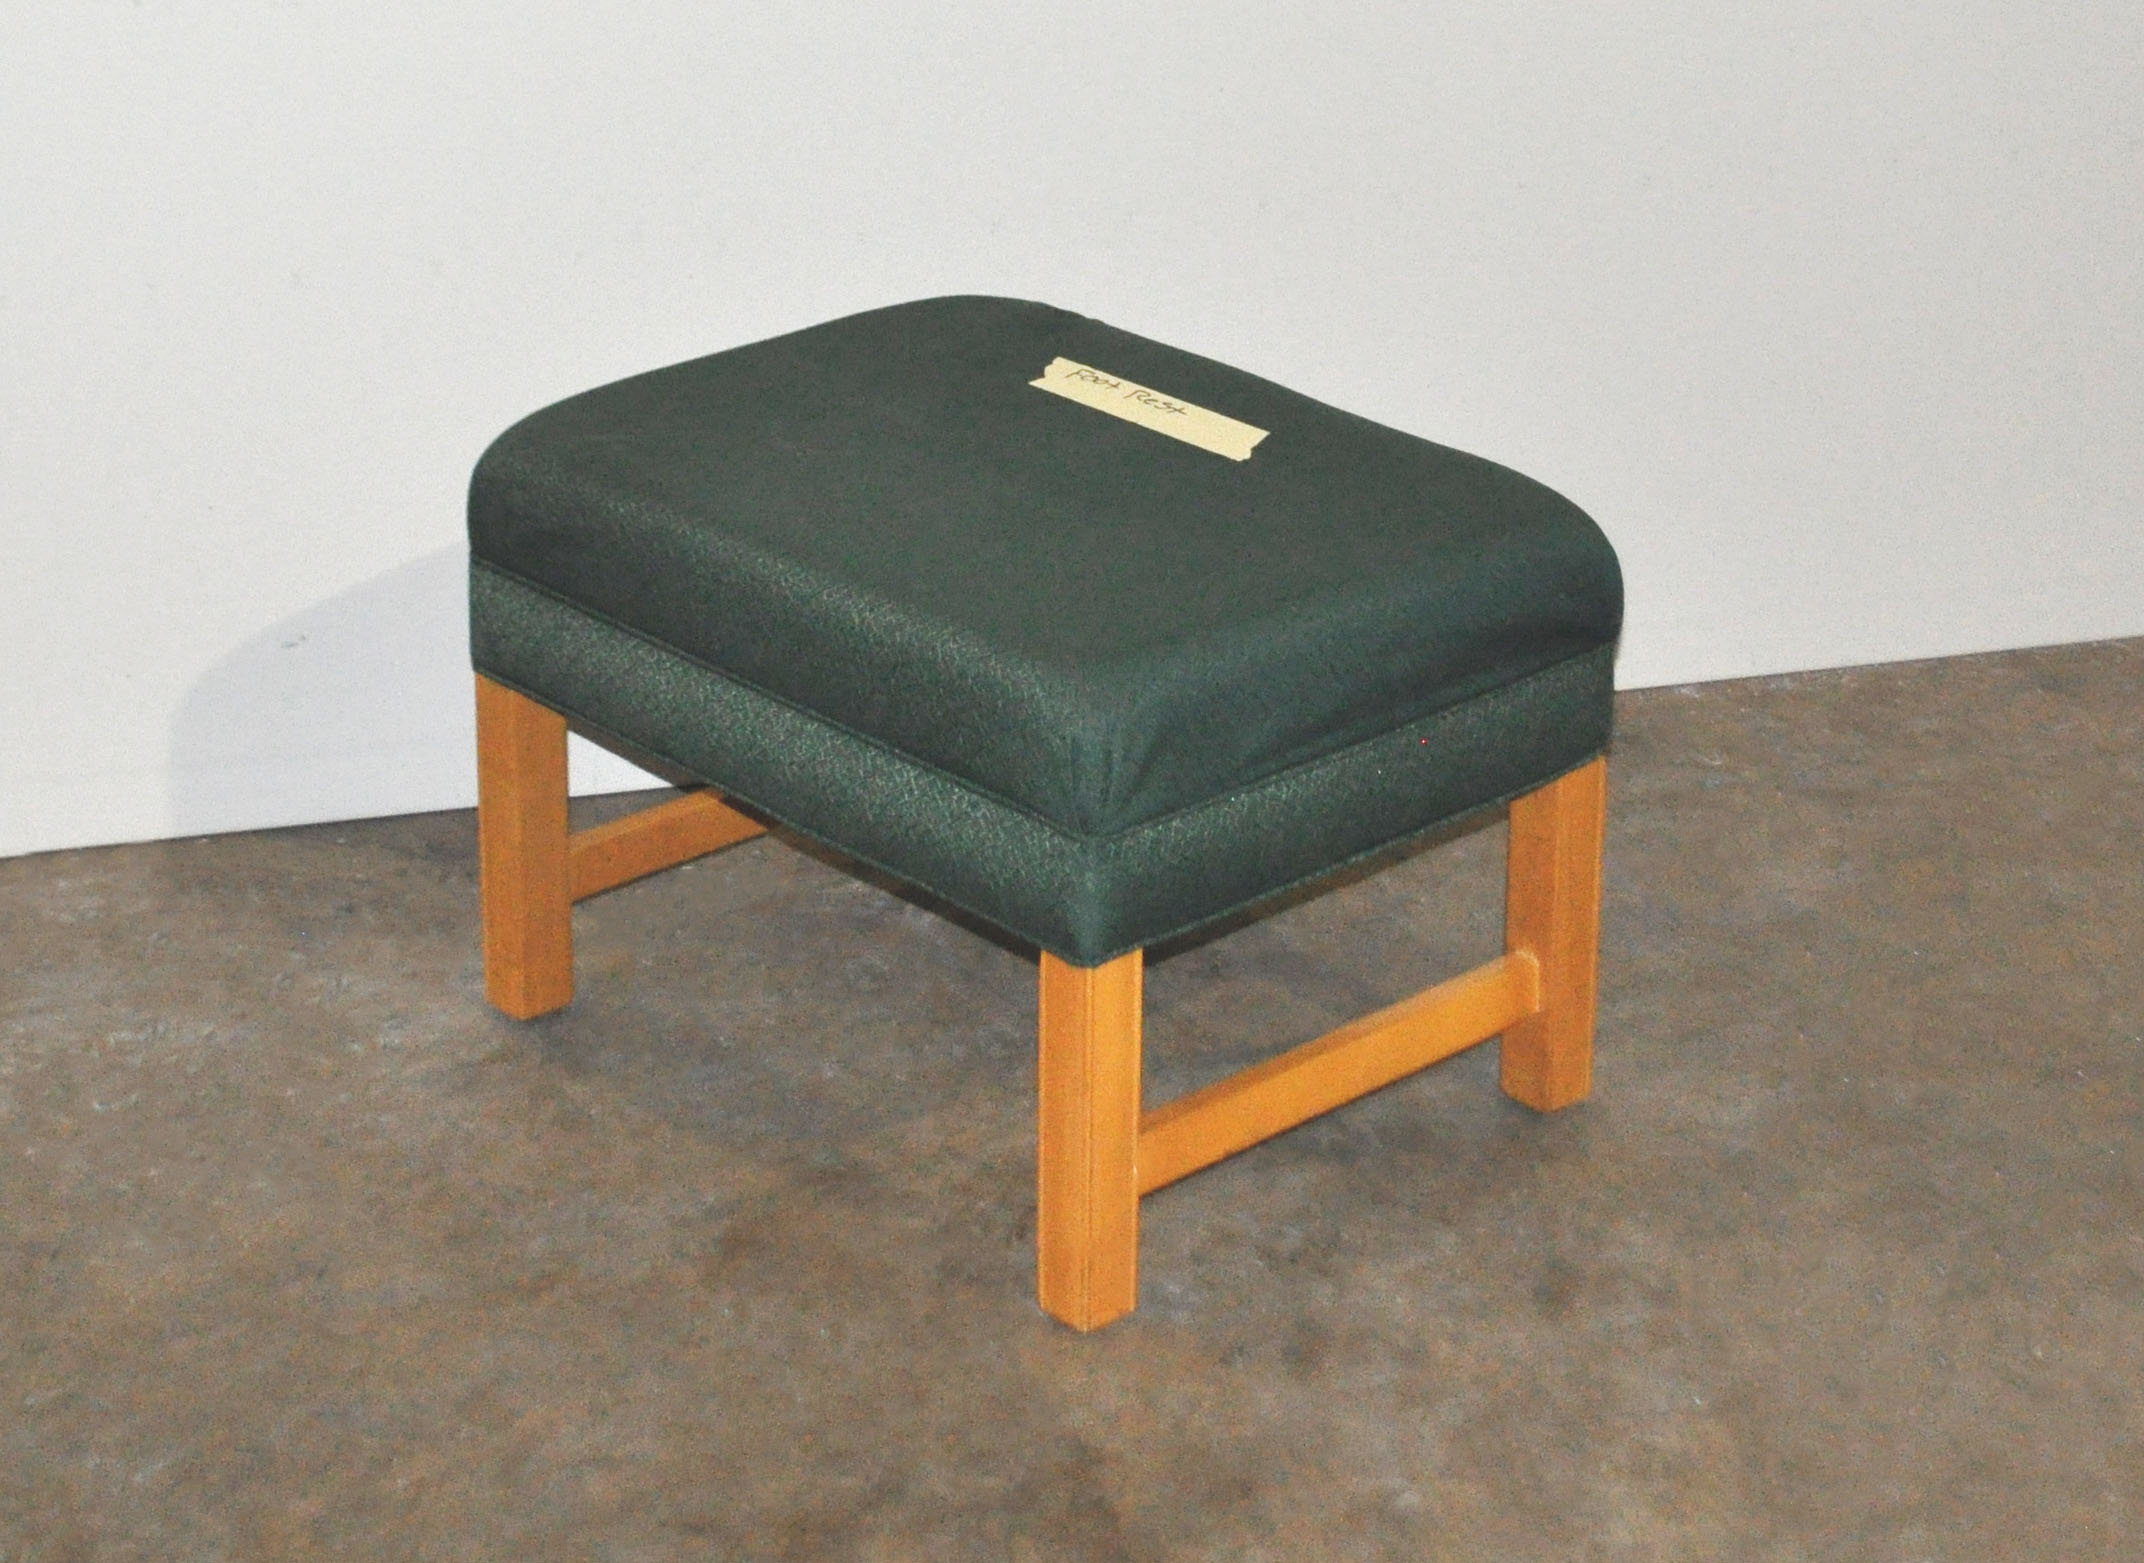
\includegraphics[width=3cm]{0_Images/Furniture/FootStool.jpg}} \\
		\subfloat[End Table]{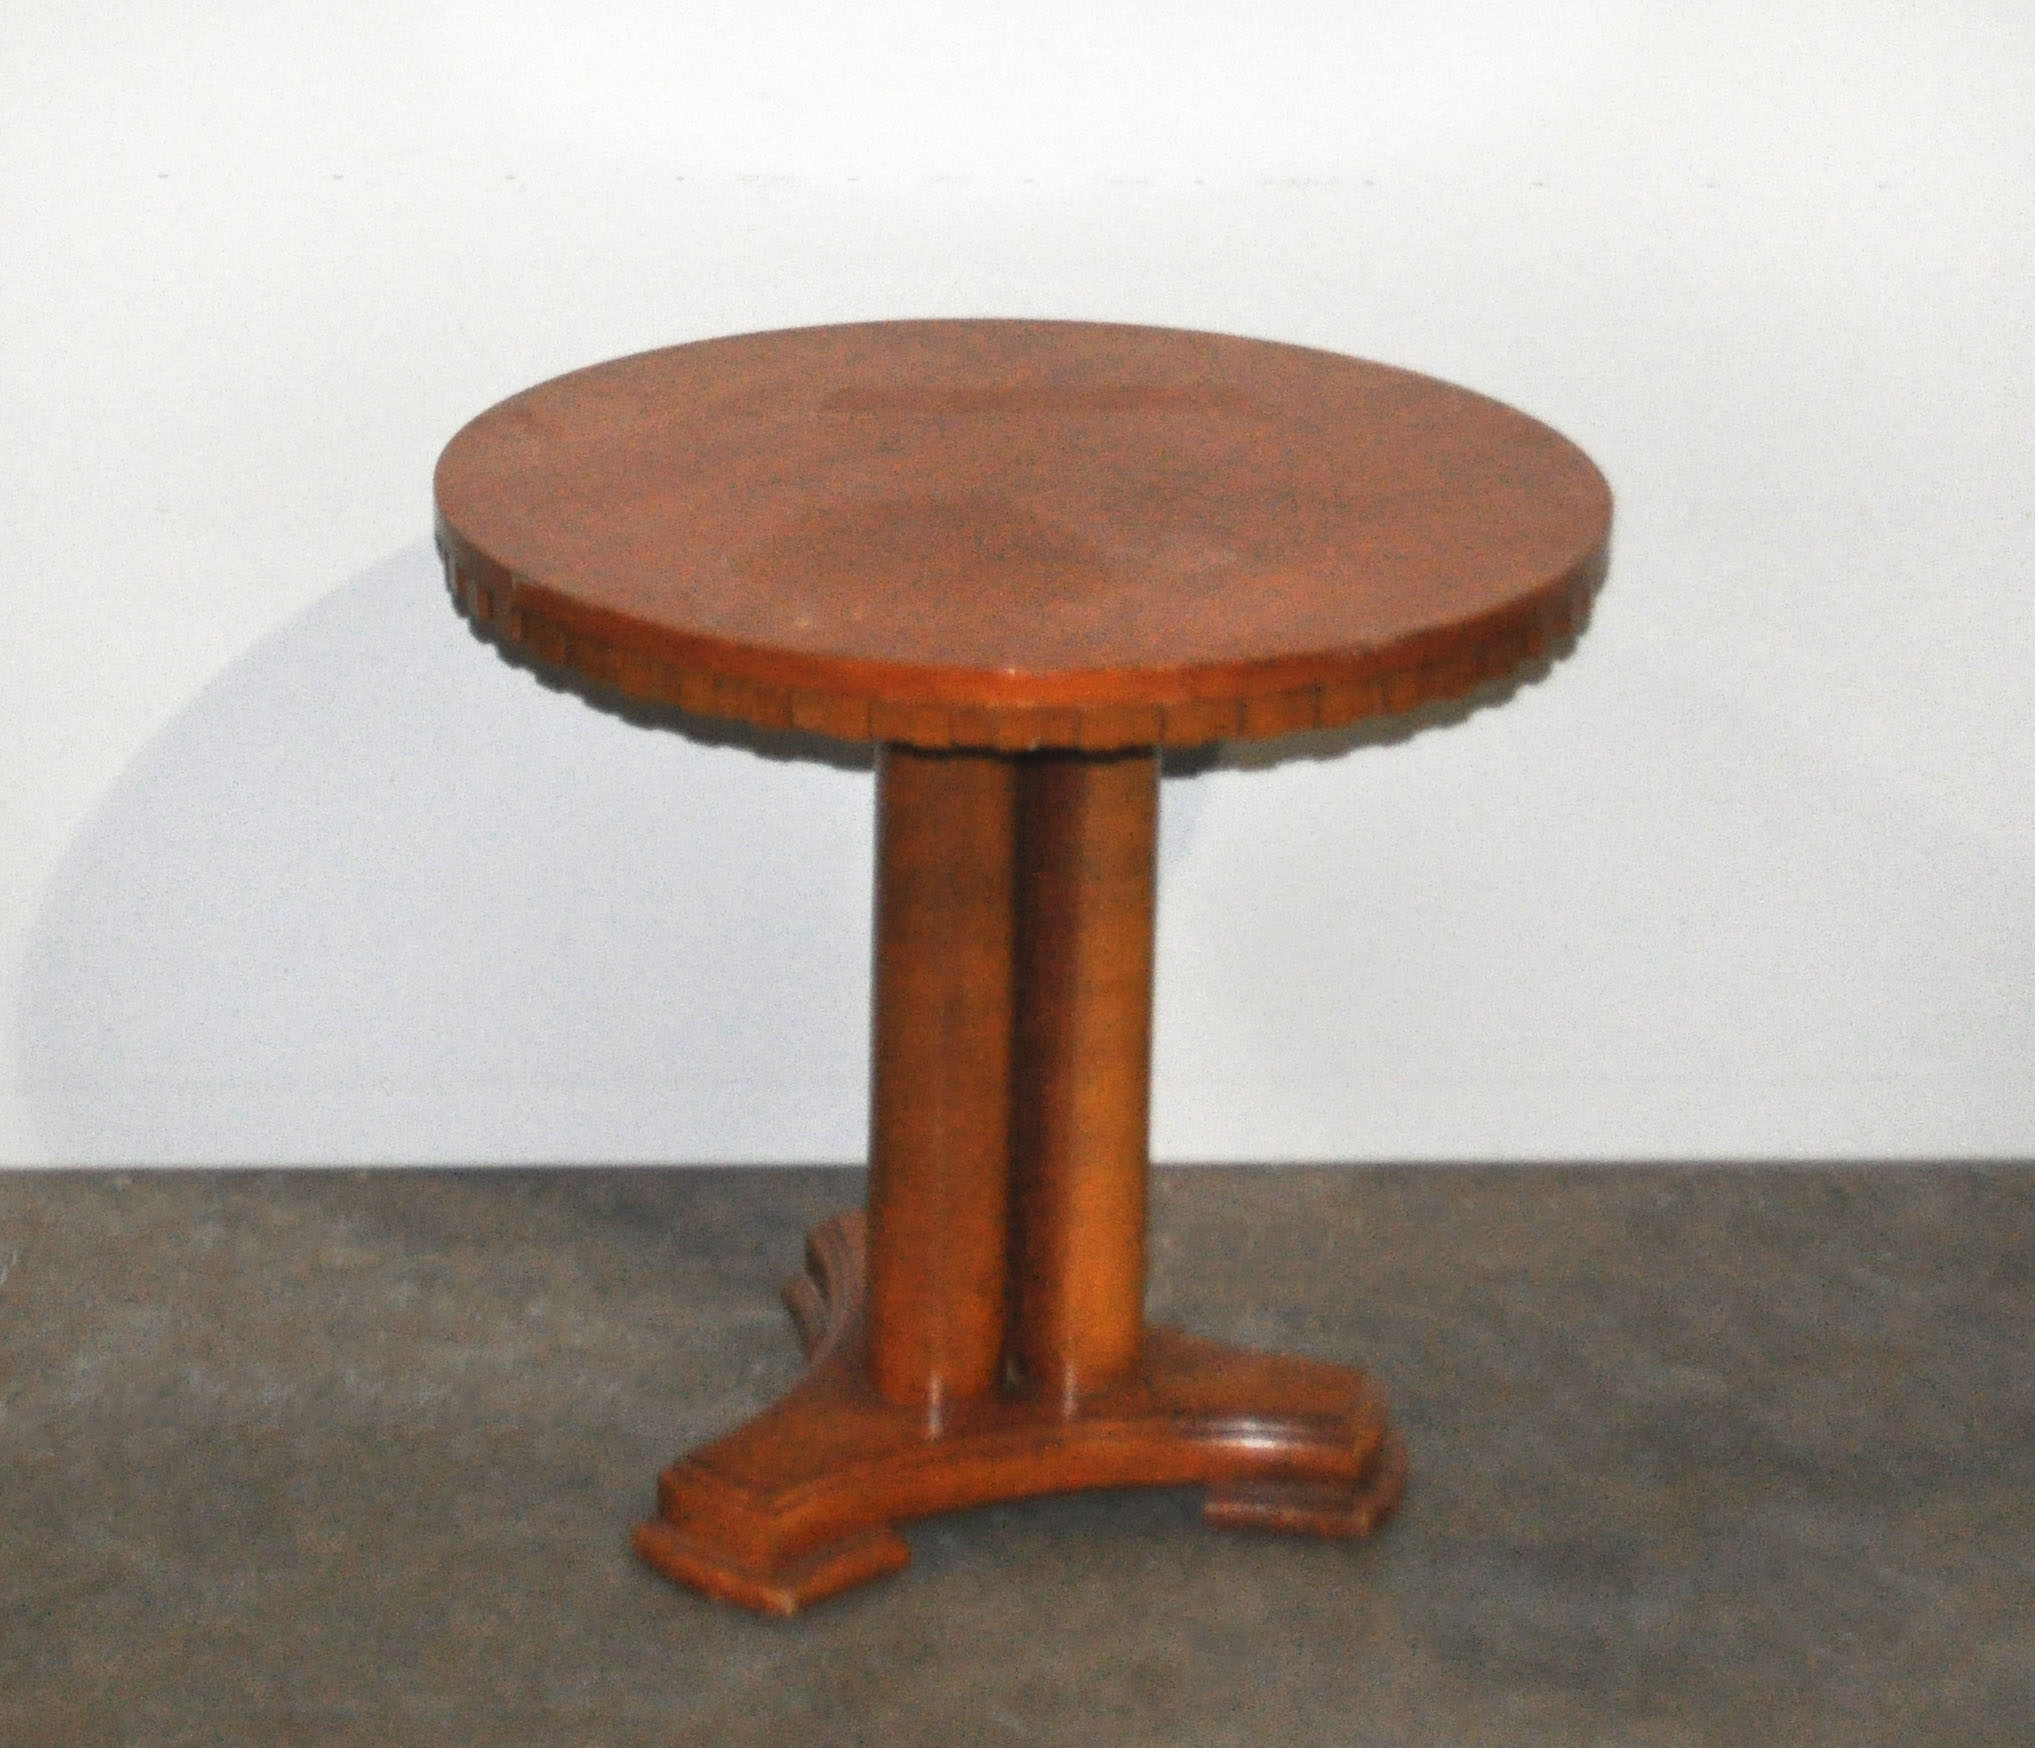
\includegraphics[width=3cm]{0_Images/Furniture/EndTable.jpg}} &
		\subfloat[Coffee Table]{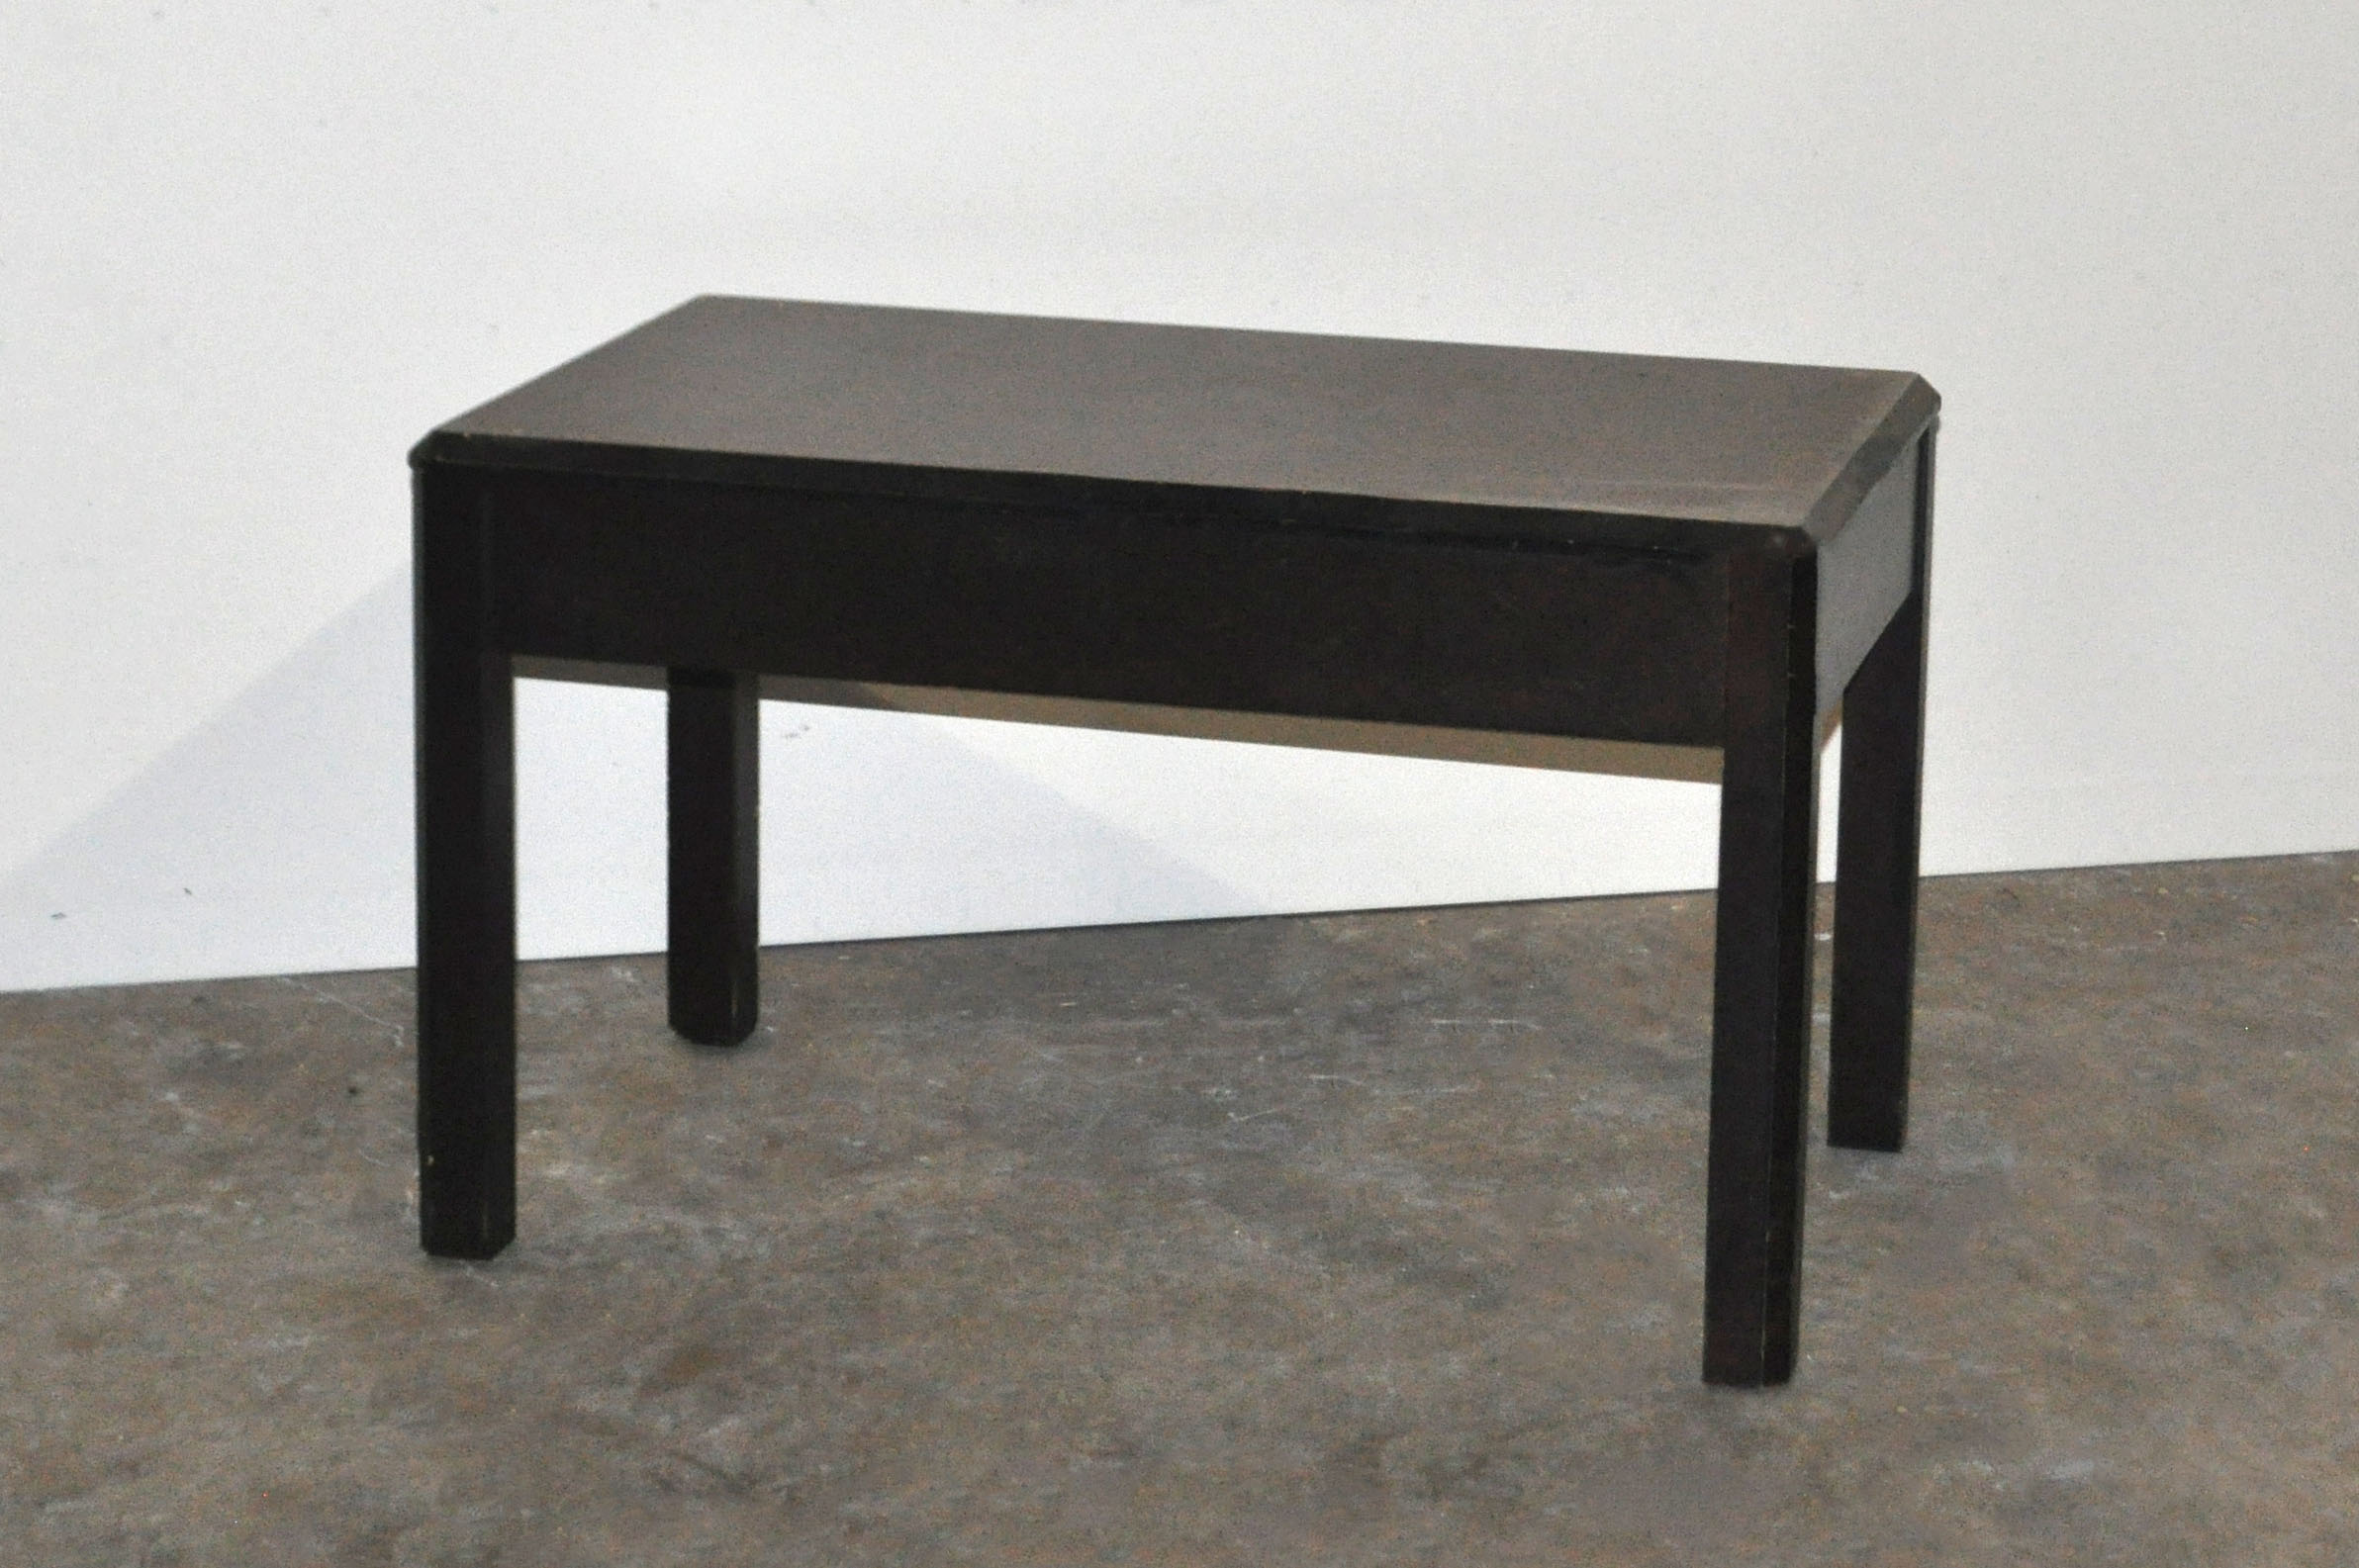
\includegraphics[width=3cm]{0_Images/Furniture/CoffeeTable.jpg}} &
		\subfloat[Lamp]{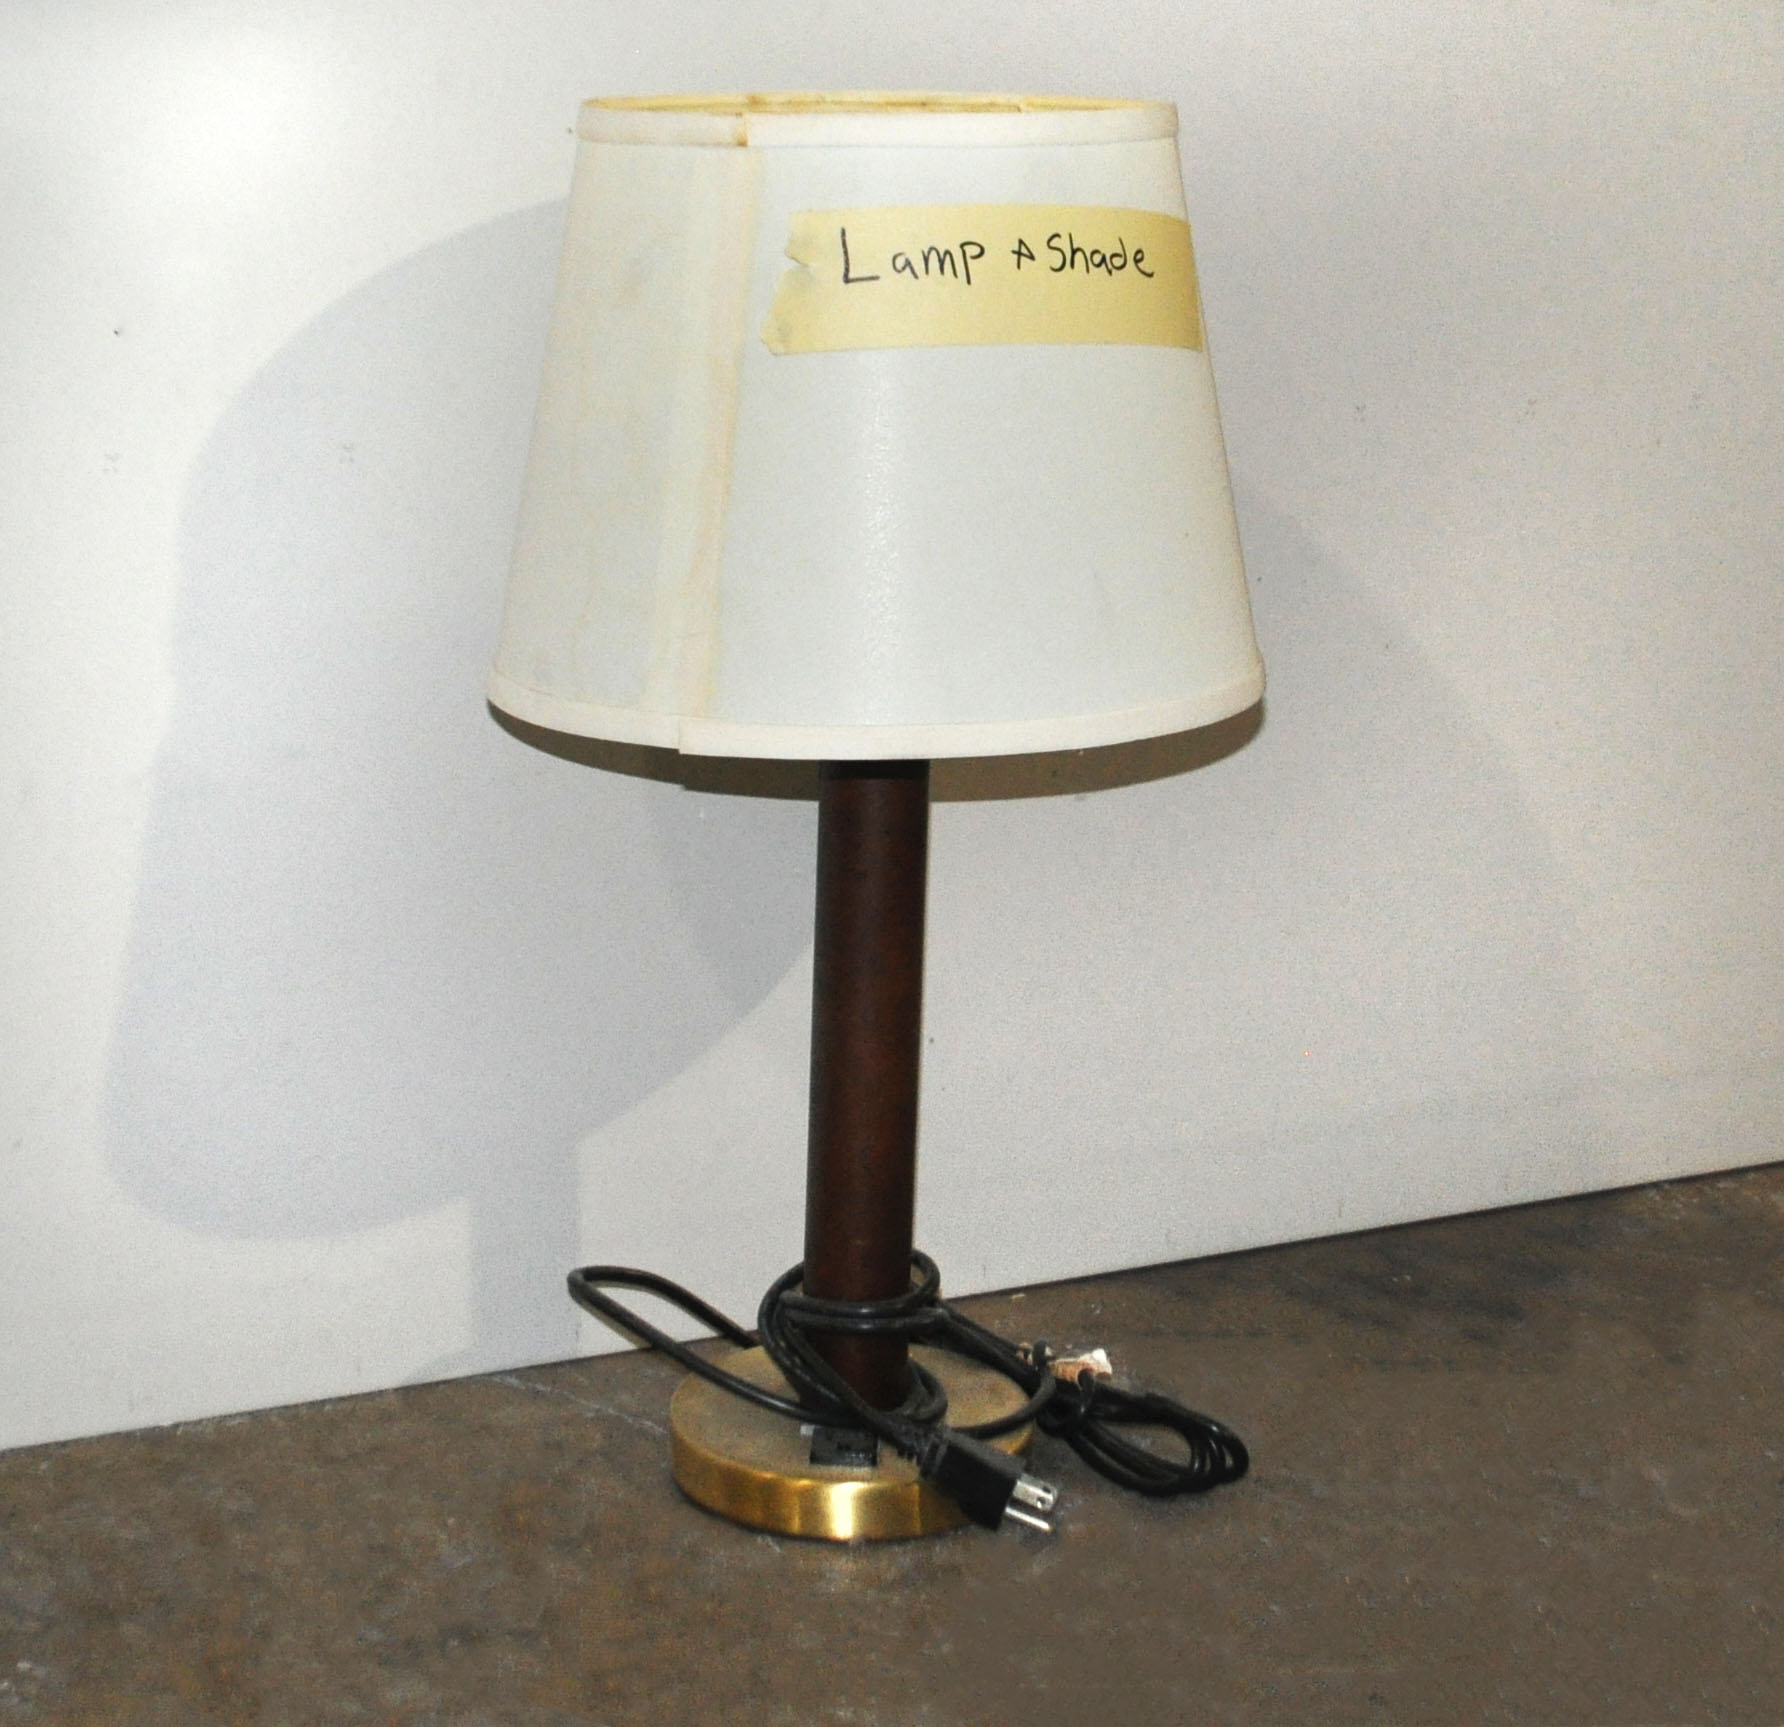
\includegraphics[width=3cm]{0_Images/Furniture/Lamp_and_Shade.jpg}} &
		\subfloat[Chair (Yellow)]{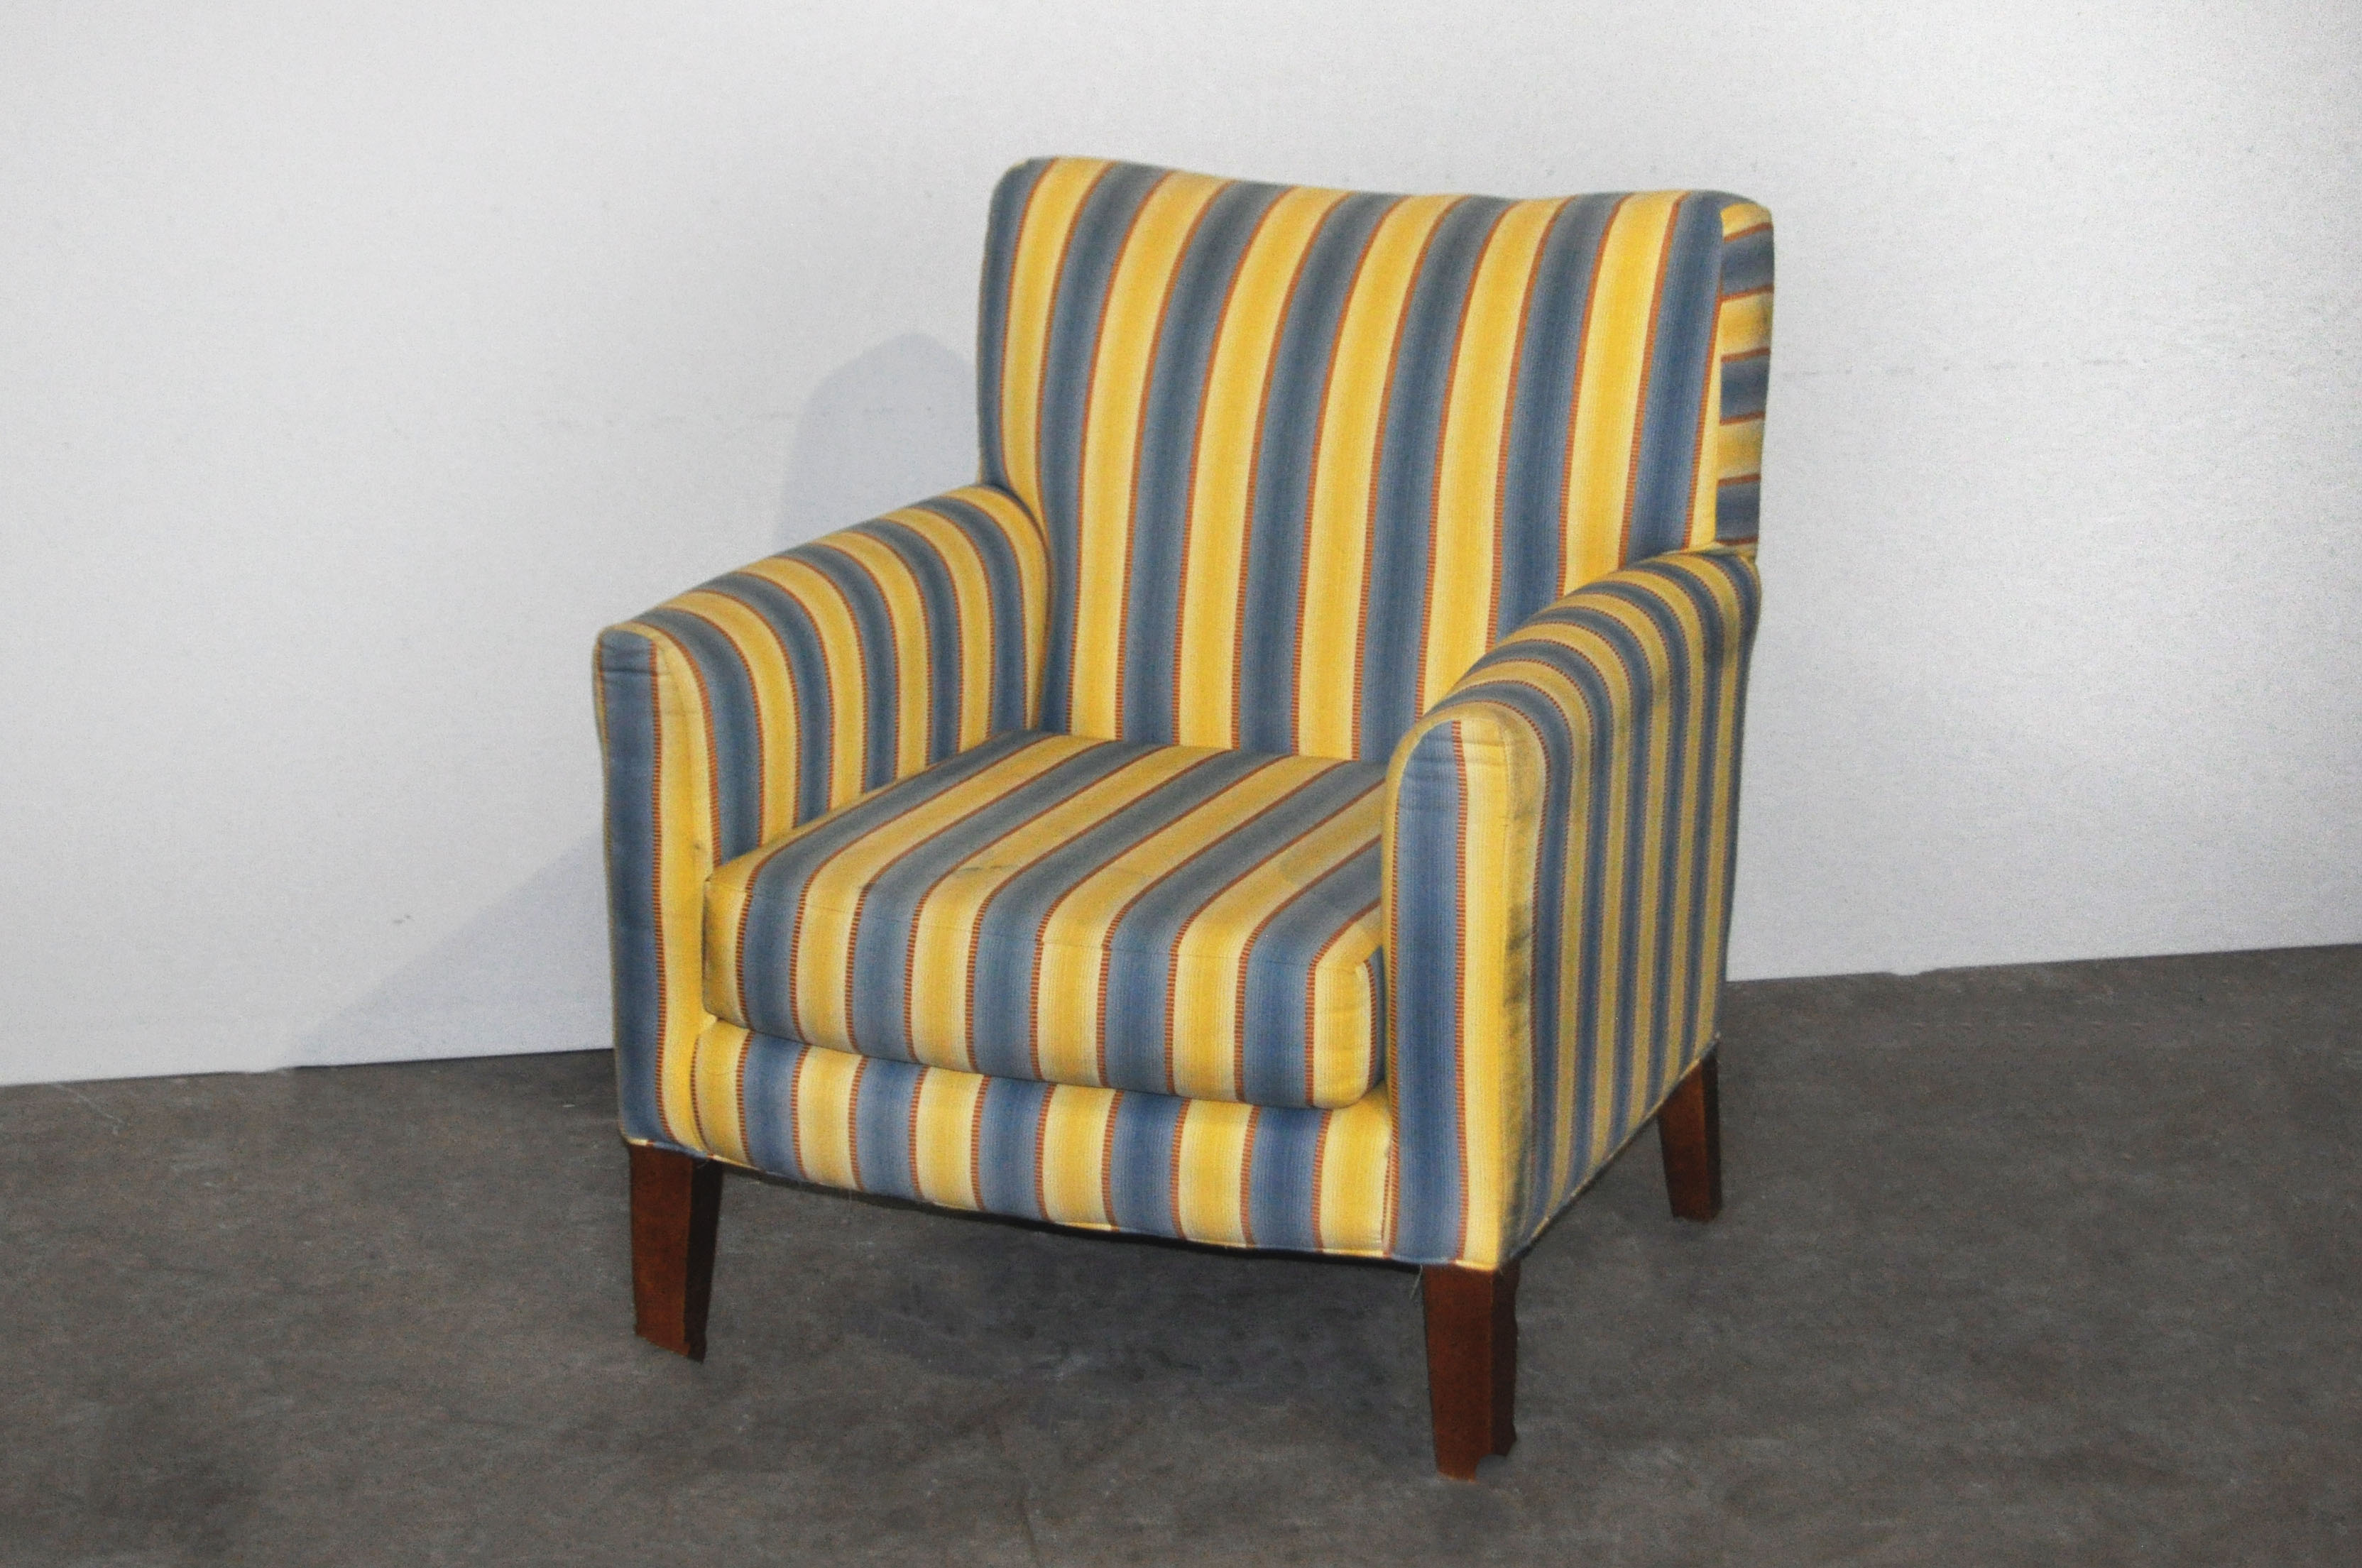
\includegraphics[width=3cm]{0_Images/Furniture/Chair(Yellow).jpg}} \\
		\subfloat[Chair (Brown)]{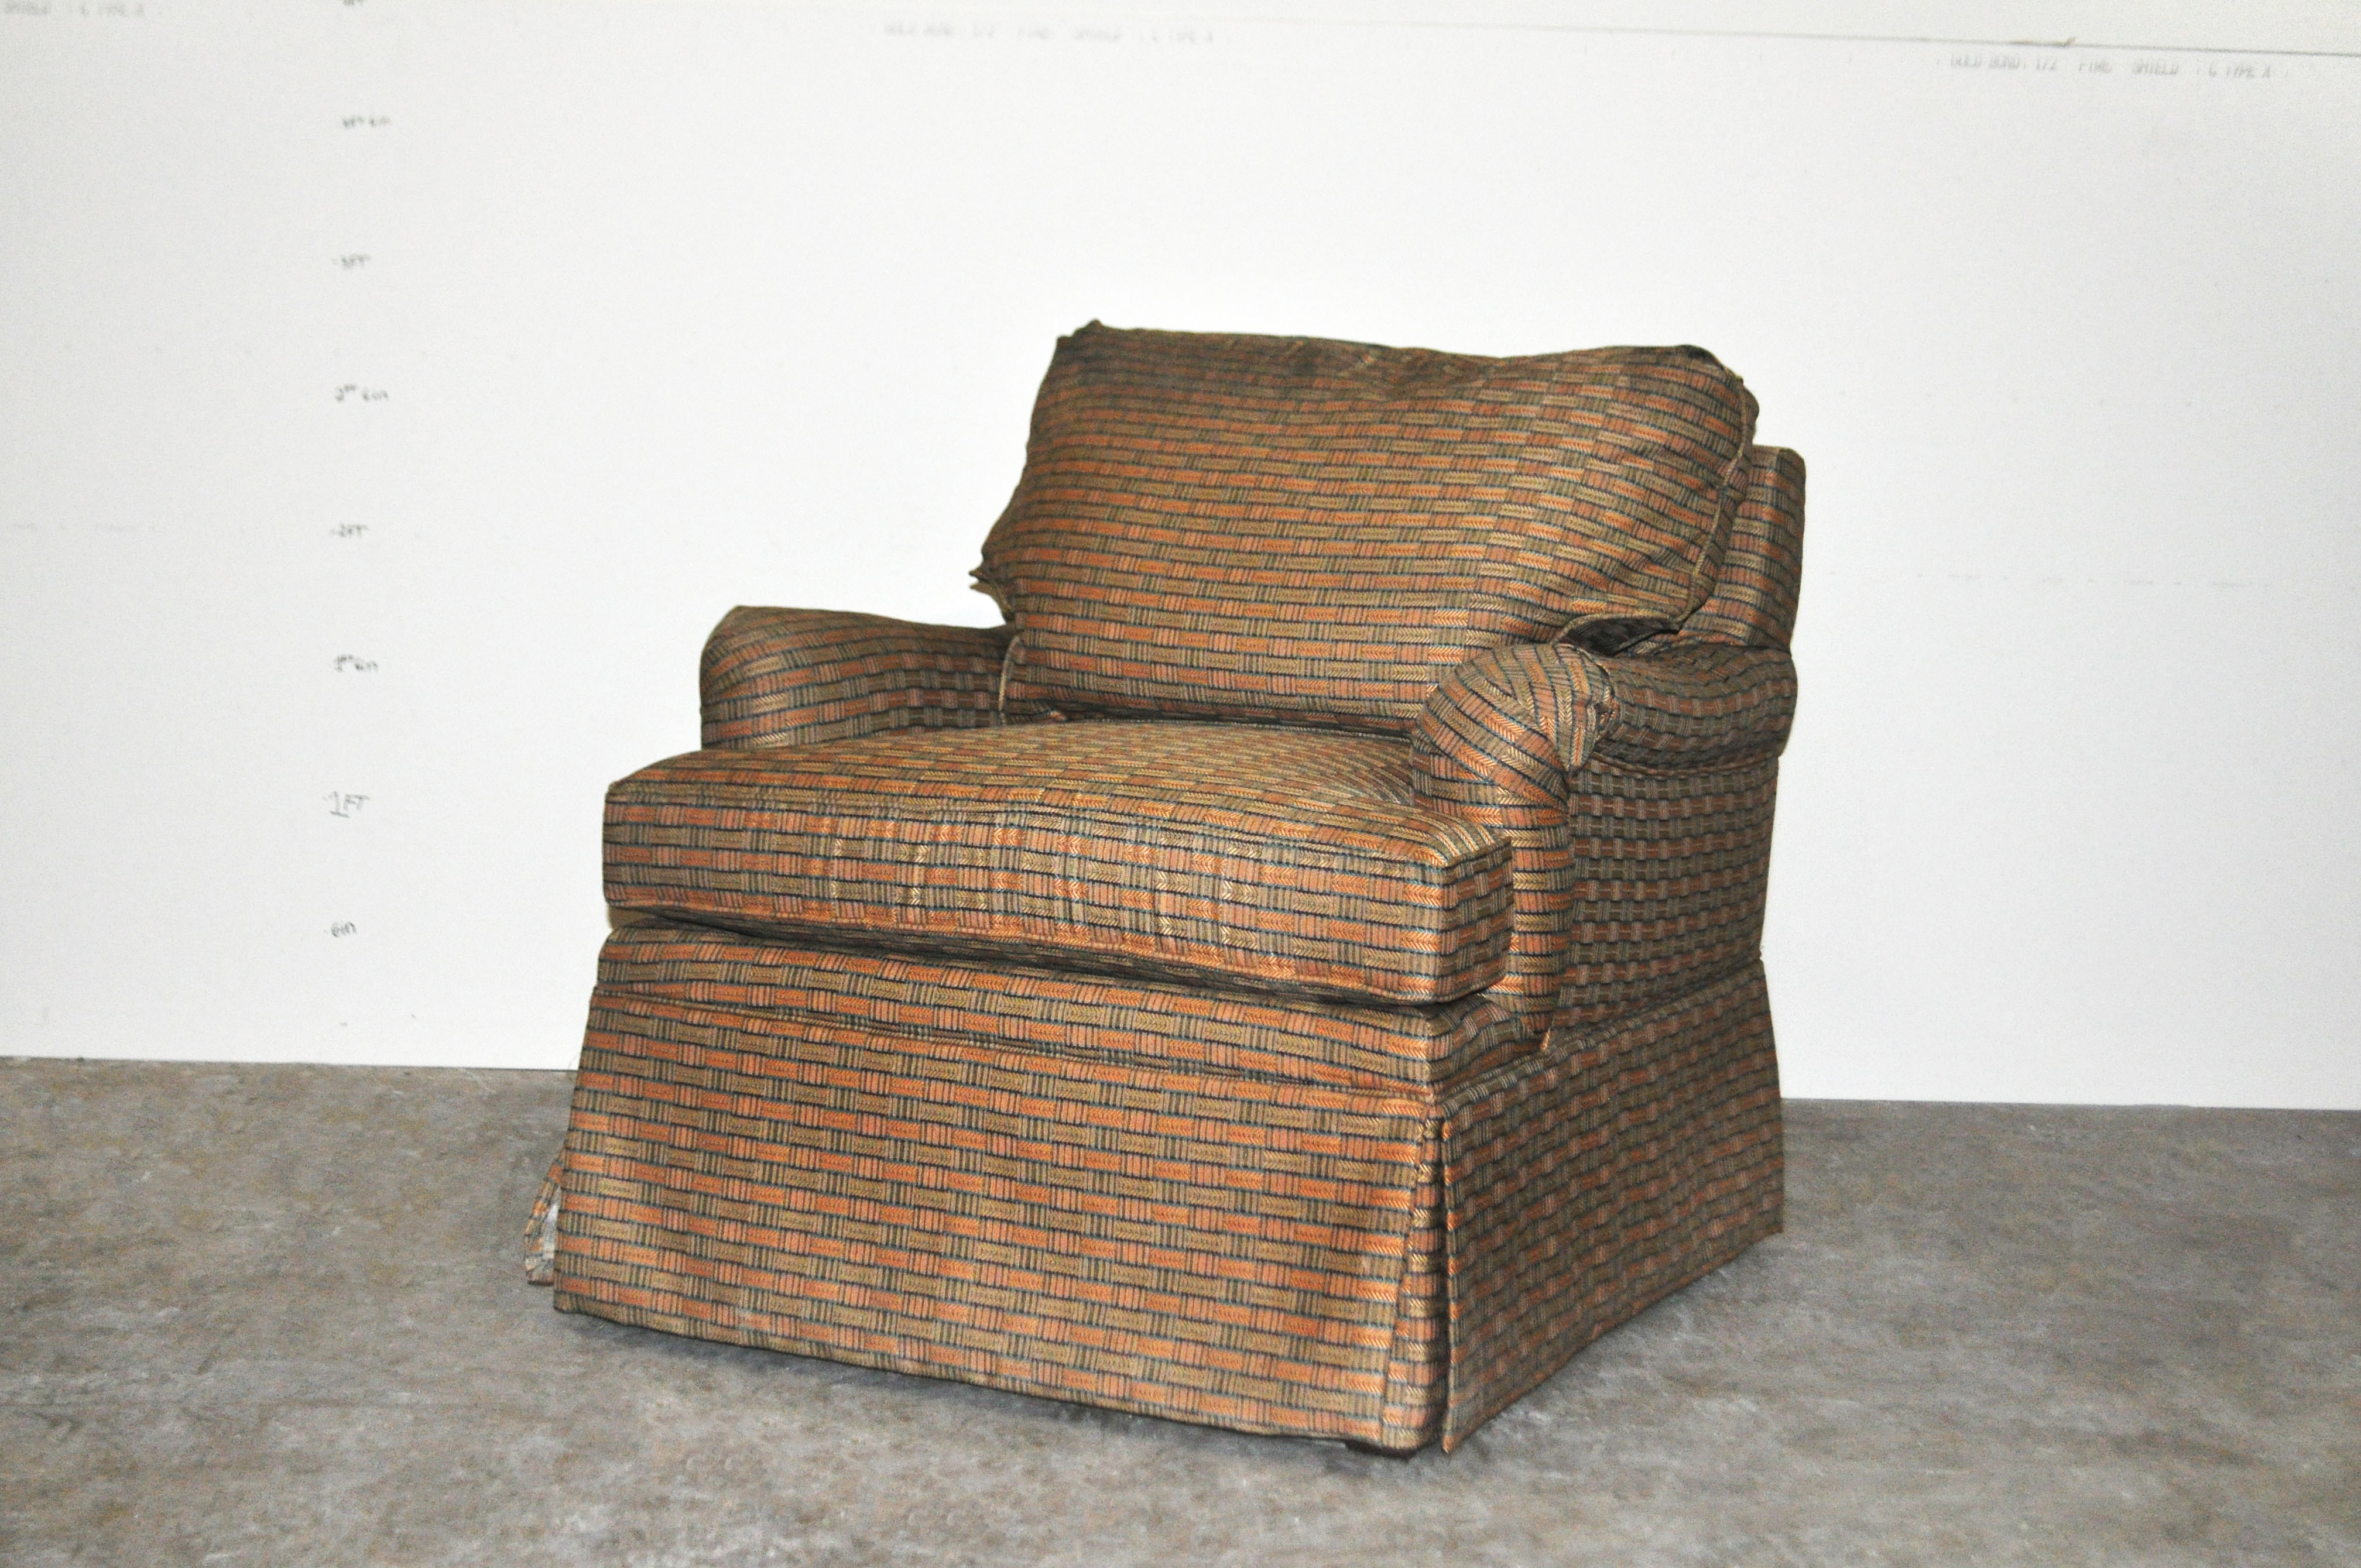
\includegraphics[width=3cm]{0_Images/Furniture/Chair(Brown).jpg}} &
		\subfloat[Sofa (Green)]{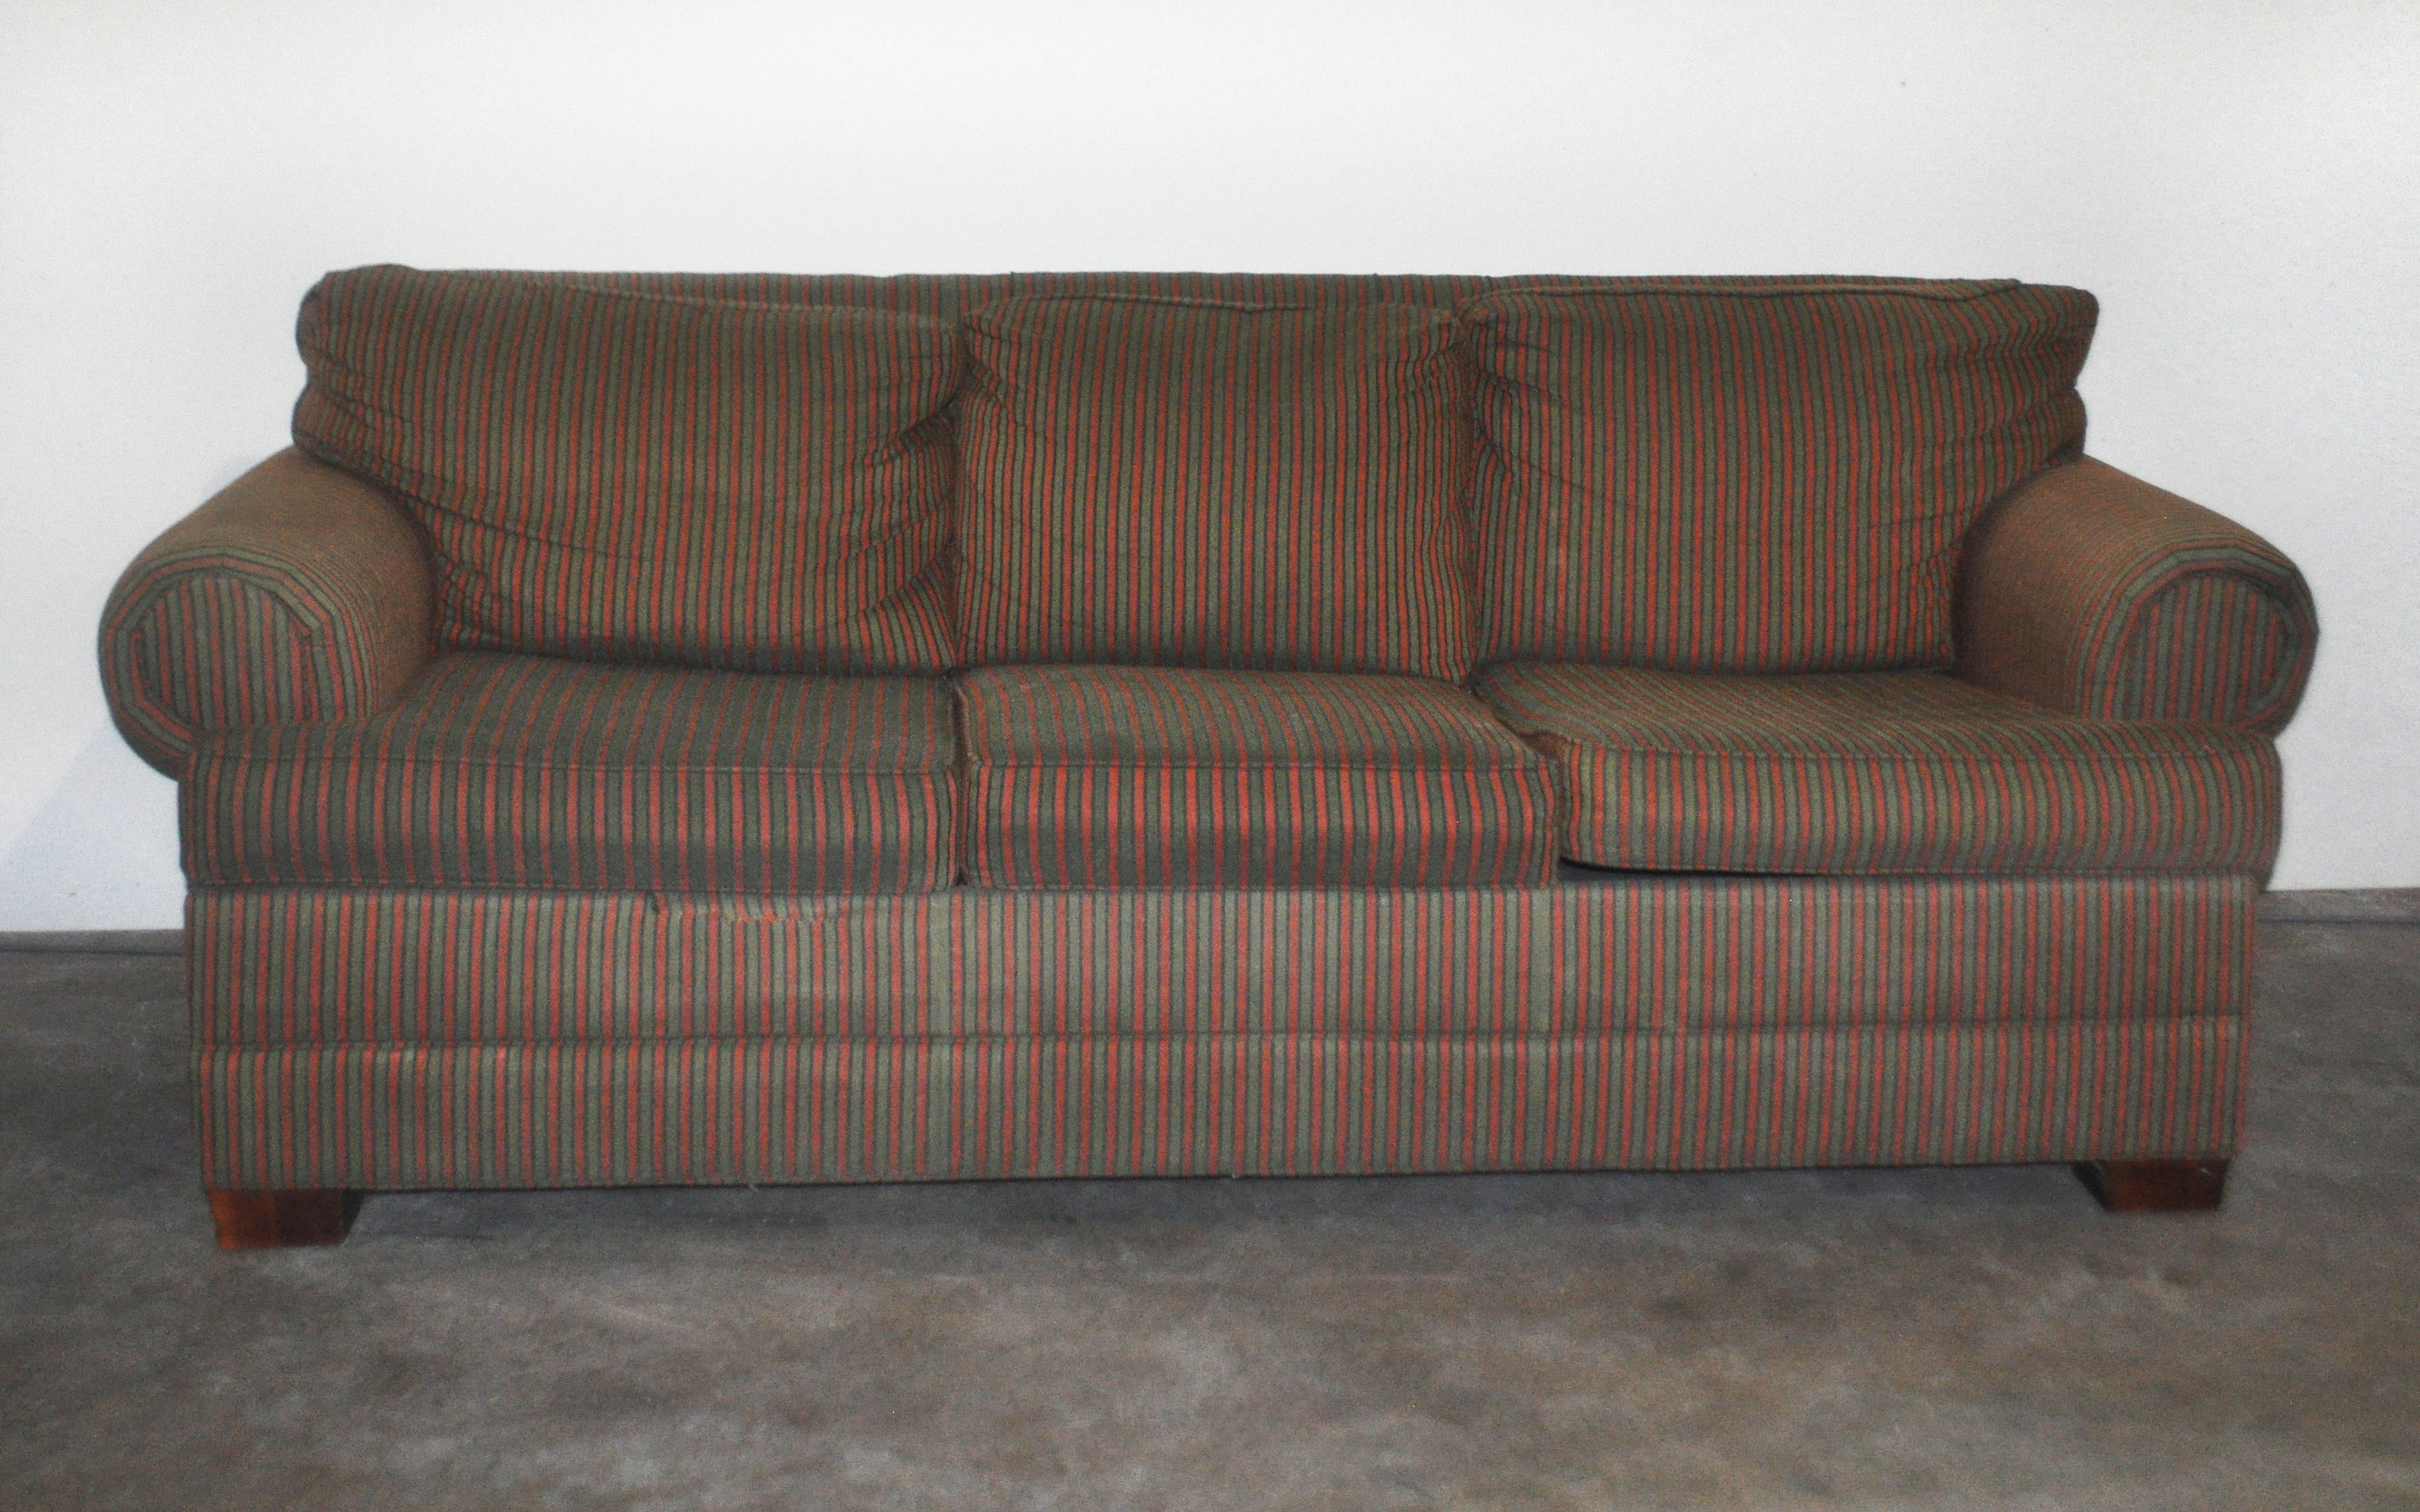
\includegraphics[width=3cm]{0_Images/Furniture/SleeperSofa(Green).jpg}} &
		\subfloat[Sofa (Orange)]{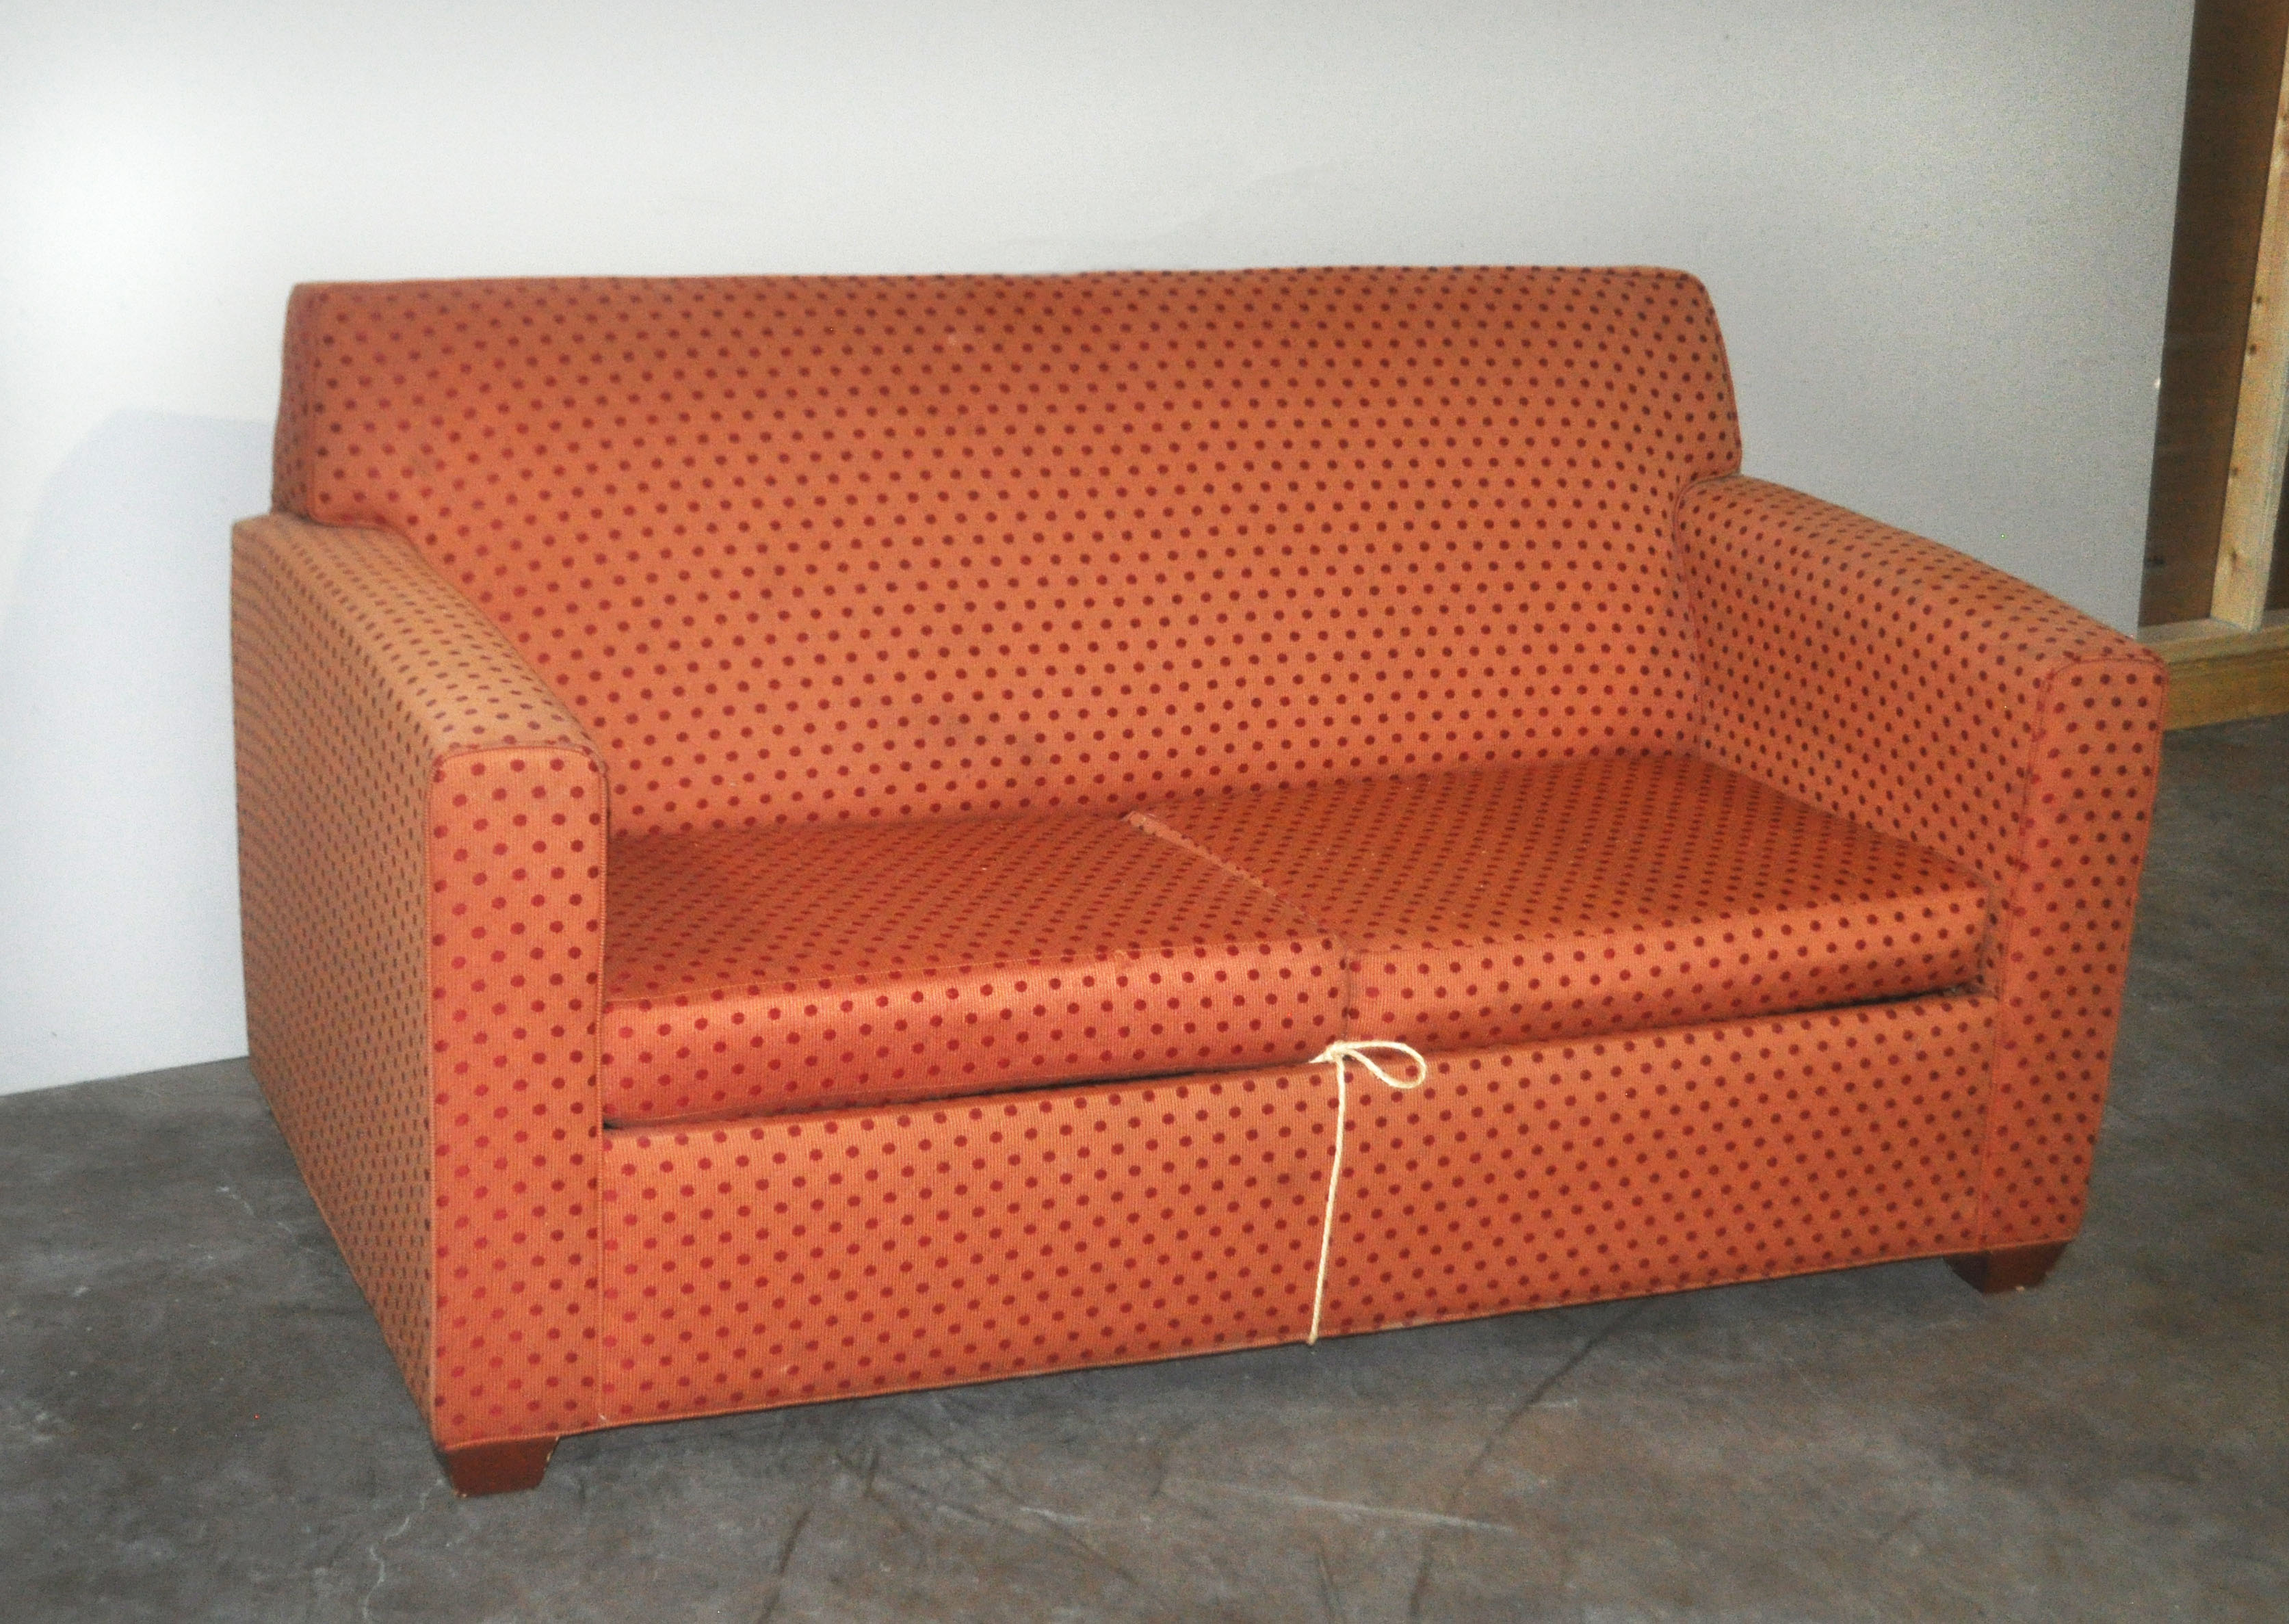
\includegraphics[width=3cm]{0_Images/Furniture/SleeperSofa(Orange).jpg}} &
		\subfloat[Curtain]{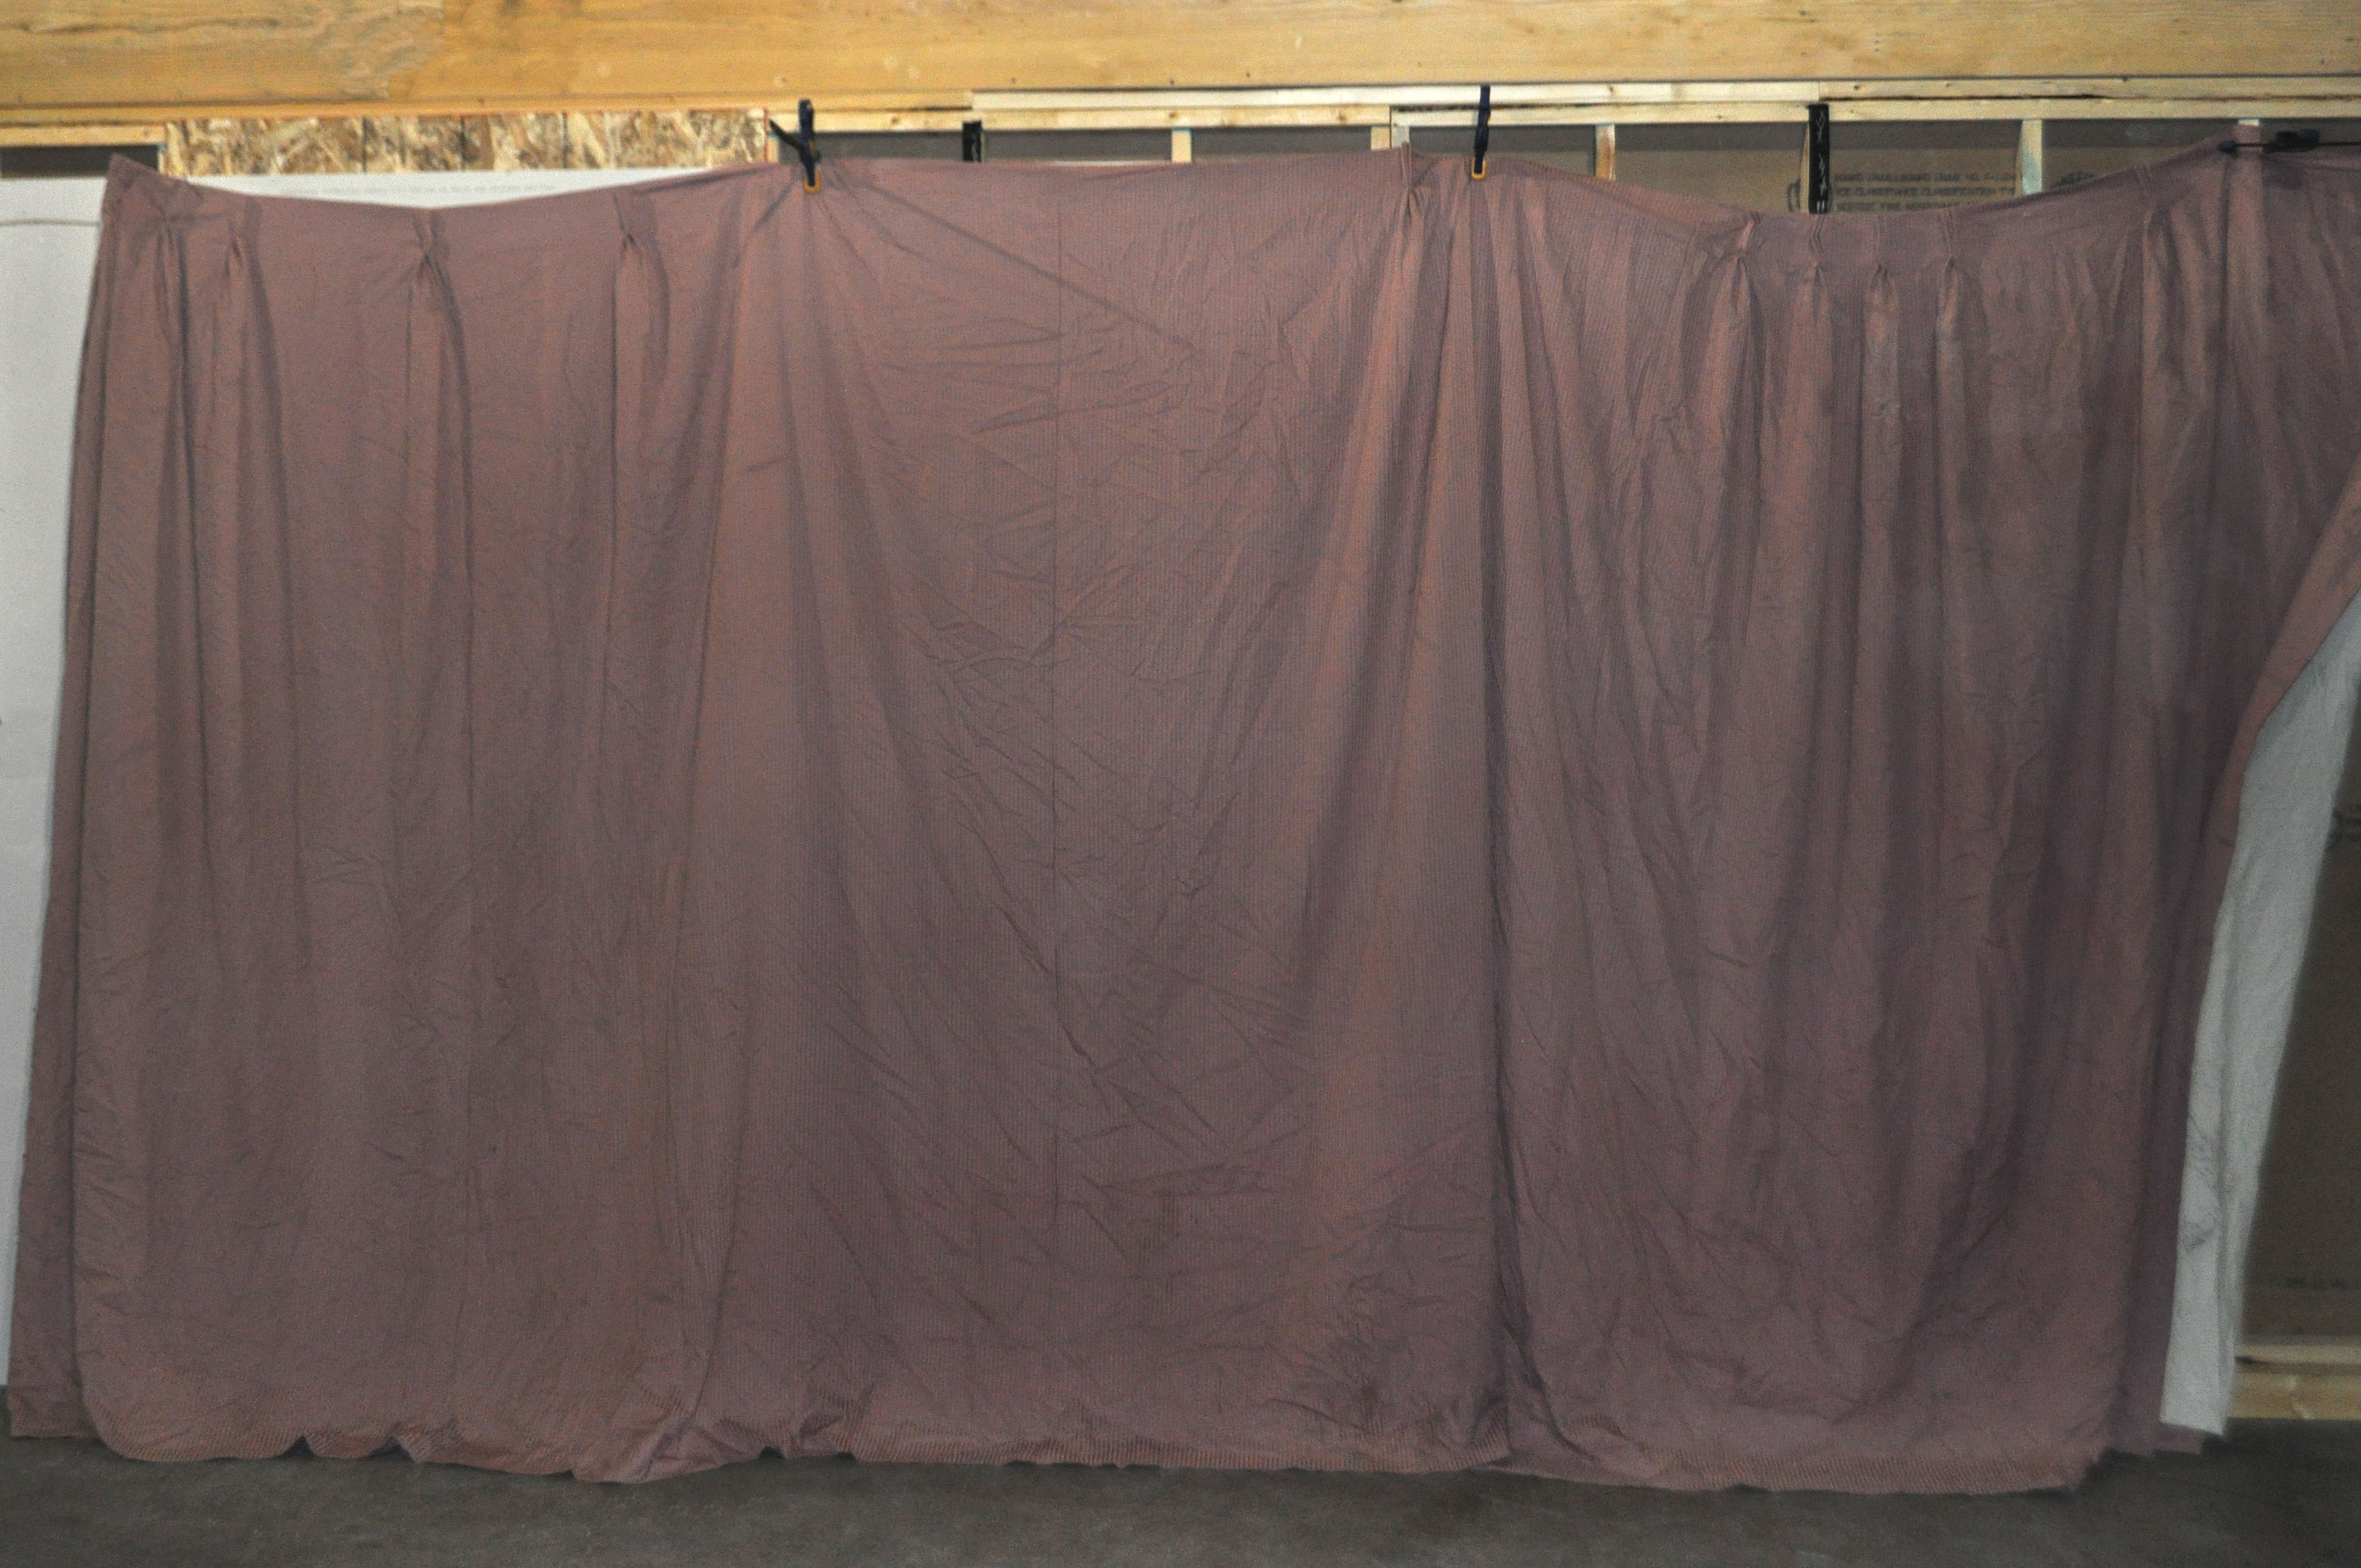
\includegraphics[width=3cm]{0_Images/Furniture/Curtian.jpg}} \\
	\end{tabular}
	\caption{Furniture Images}
	\label{fig:FurnitureImages}
\end{figure}


The living room in the one-story house, as well as the family room and the living room in the two-story house, was furnished similarly with two sofas, armoire, television, television stand, ottoman, end table, coffee table, chair, two pictures, lamp with shade and two curtains .  The floor was covered with polyurethane foam padding and polyester carpet. Figure \ref{fig:Living_Family} shows both the single story living room and two story family room furniture setup.  

\begin{figure}[H]
	\centering
	\begin{tabular}[c]{c c}
		\subfloat[Single Story Living Room]{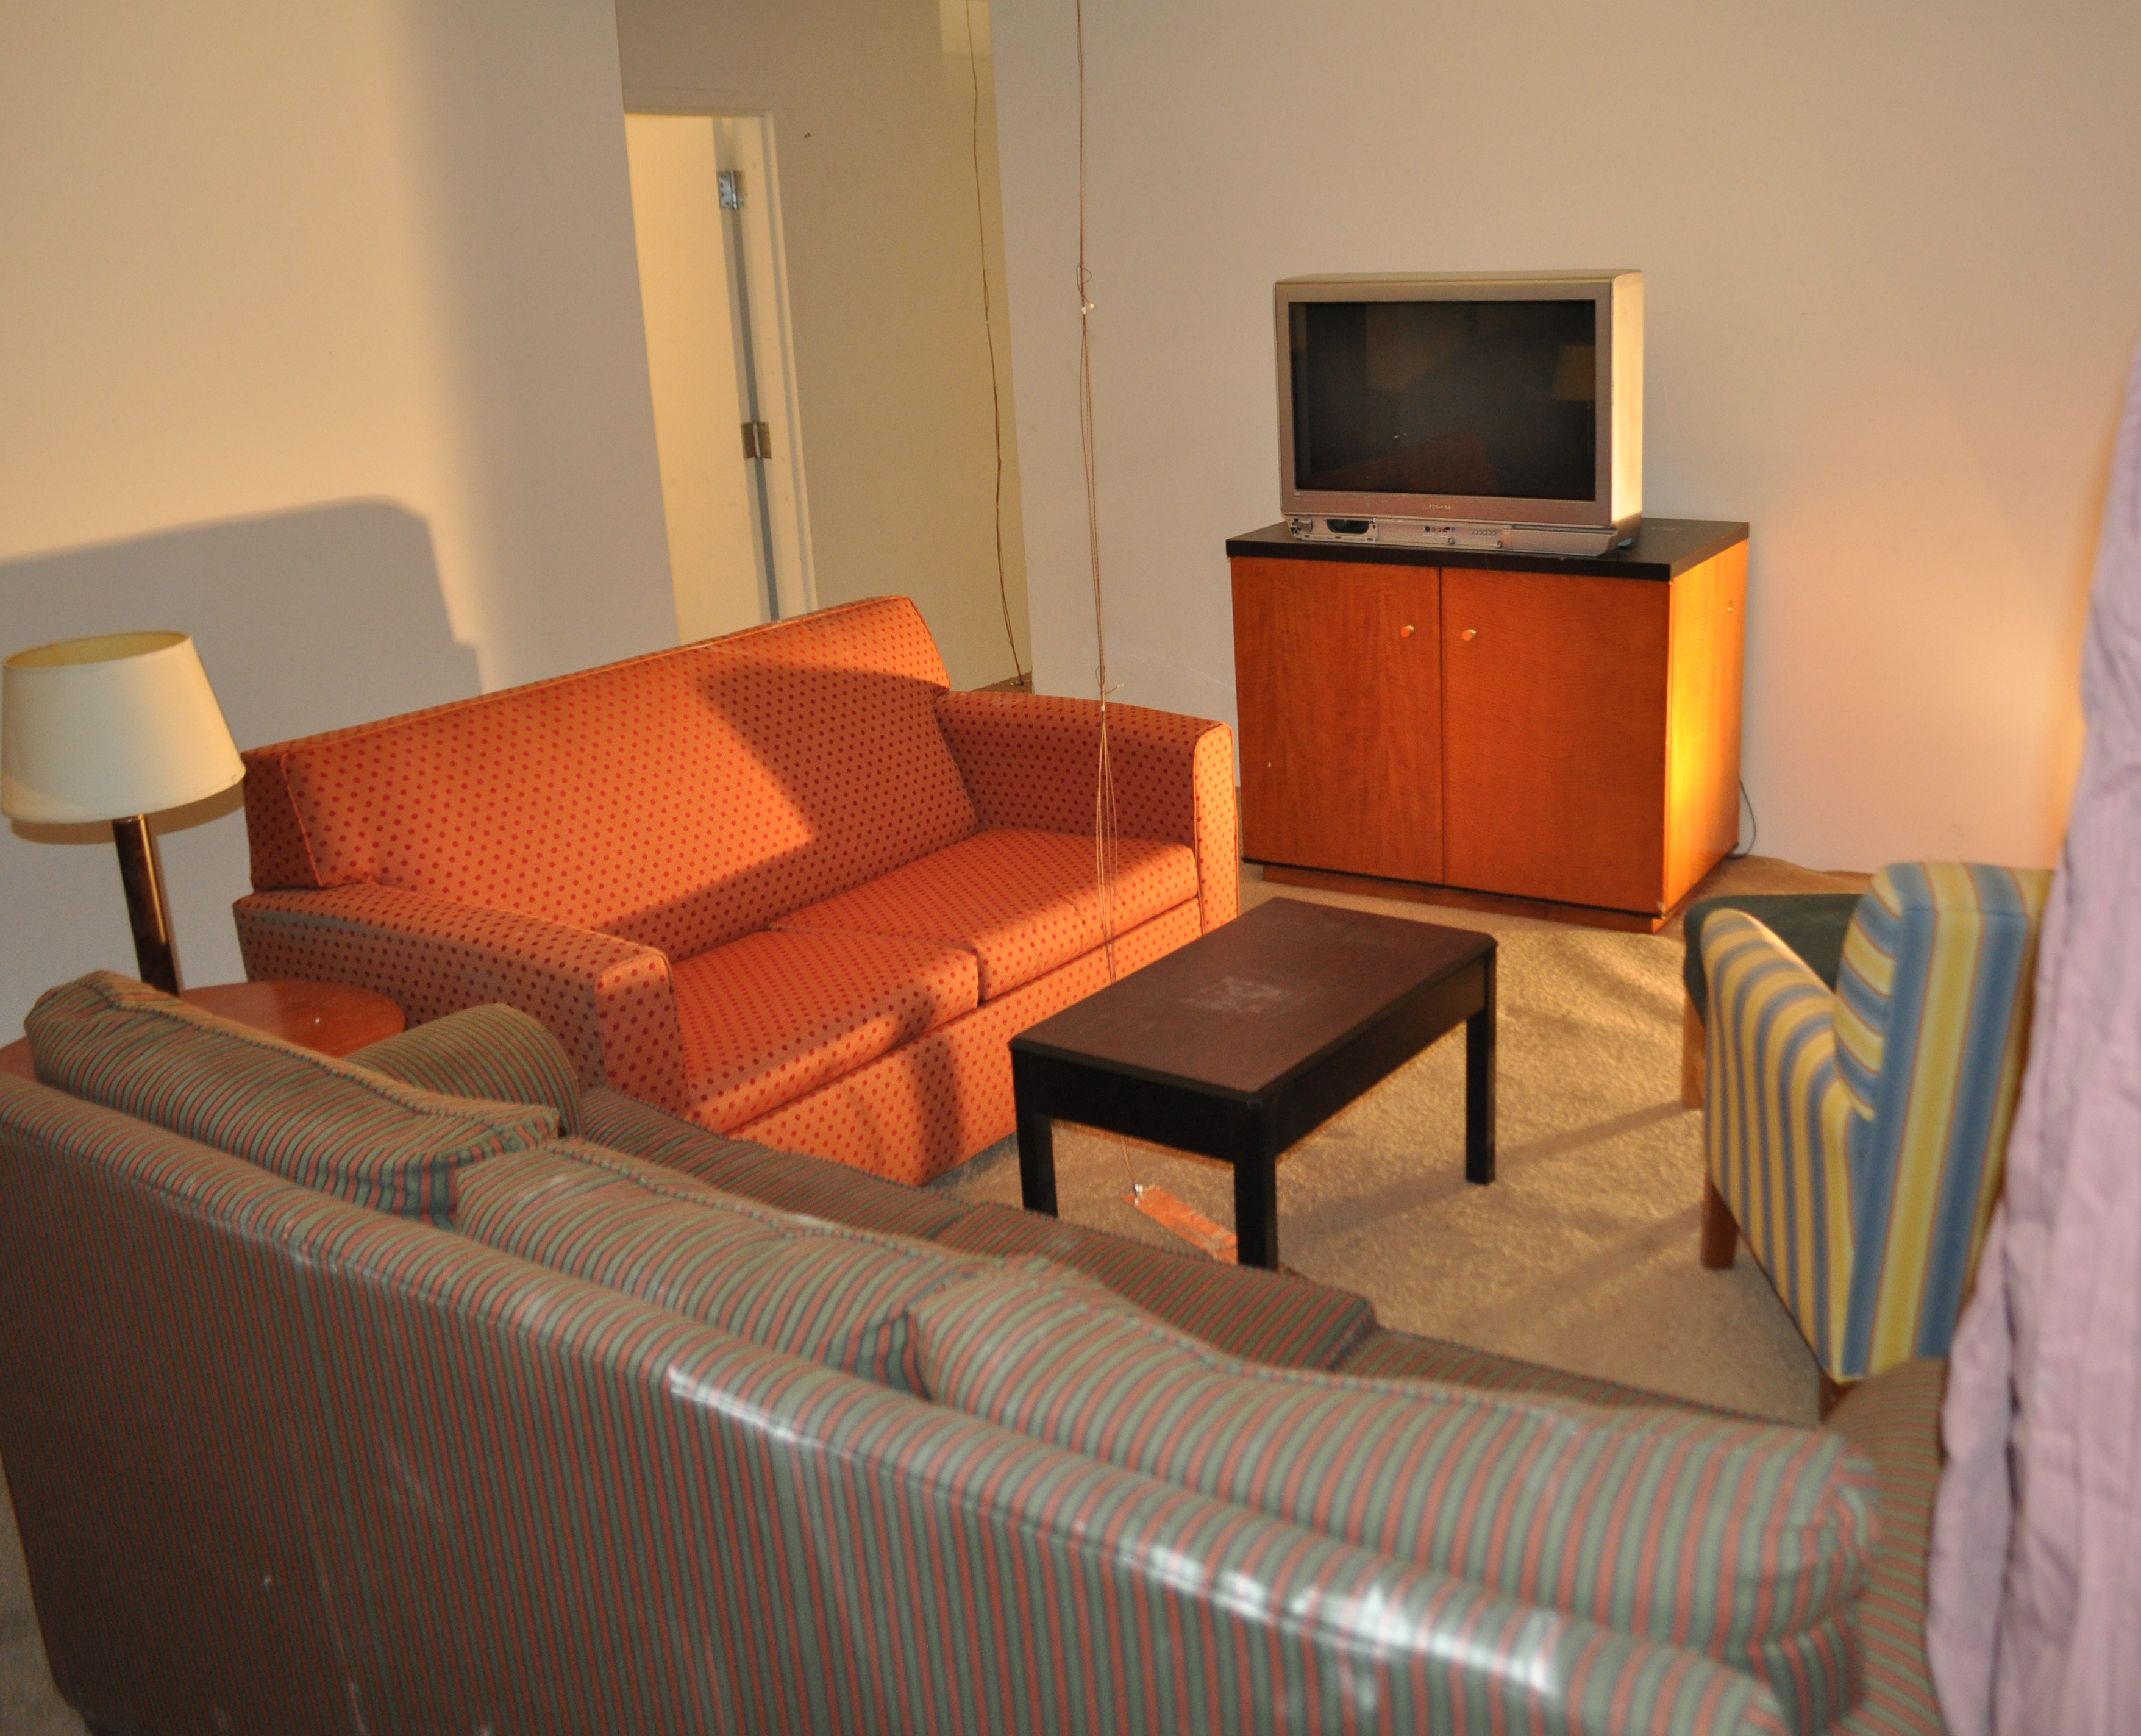
\includegraphics[width=3in]{0_Images/Furniture/SingleStoryLivingRoom.jpg}} &
		\subfloat[Two Story Family Room]{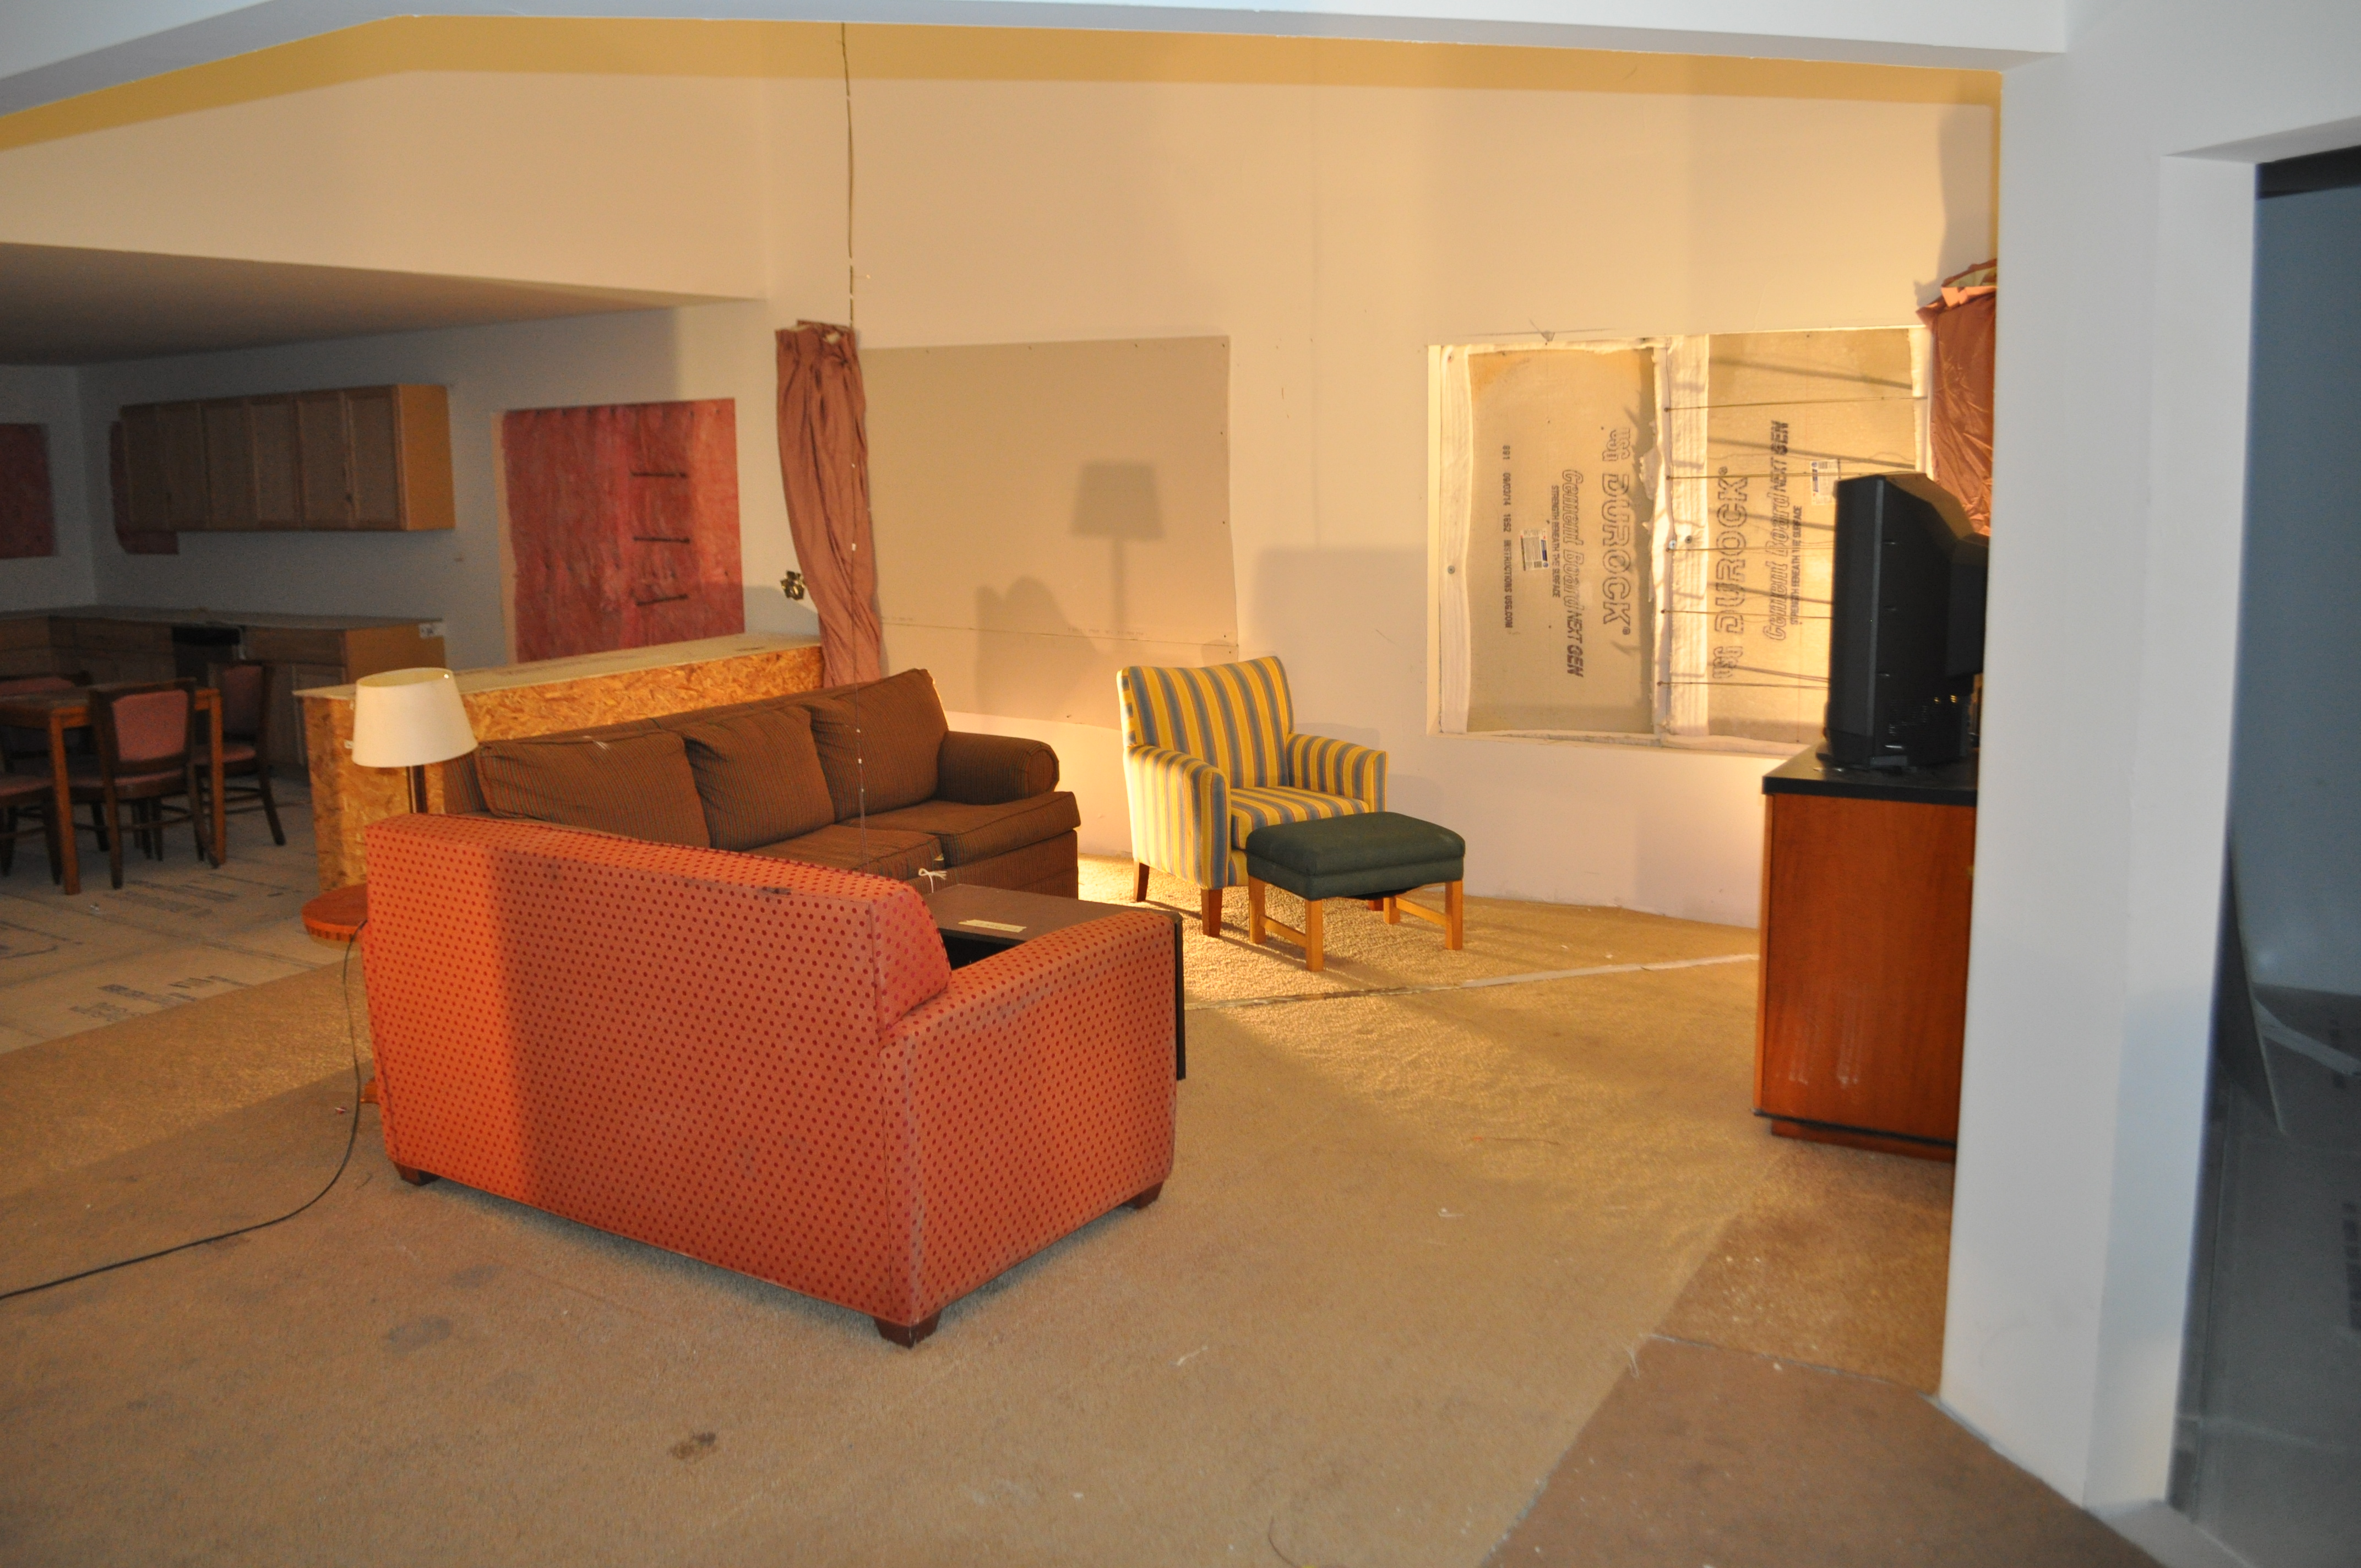
\includegraphics[width=3in]{0_Images/Furniture/TwoStoryFamilyRoom.jpg}} \\
	\end{tabular}
	\caption{Living \& Family Room Furniture}
	\label{fig:Living_Family}
\end{figure}

The master bedroom in both houses was furnished with a queen bed comprised of a mattress, box spring, wood frame, two pillows and comforter.  The rest of the room had a dark brown dresser and television. In th Single Story the master bedroom also contained a brown chair.  The floor was covered with polyurethane foam padding and polyester carpet. Figure XX shows the master bedroom furniture setup in both the single story and two story.

\begin{figure}[H]
	\centering
	\begin{tabular}[c]{c c}
		\subfloat[Single Story Master]{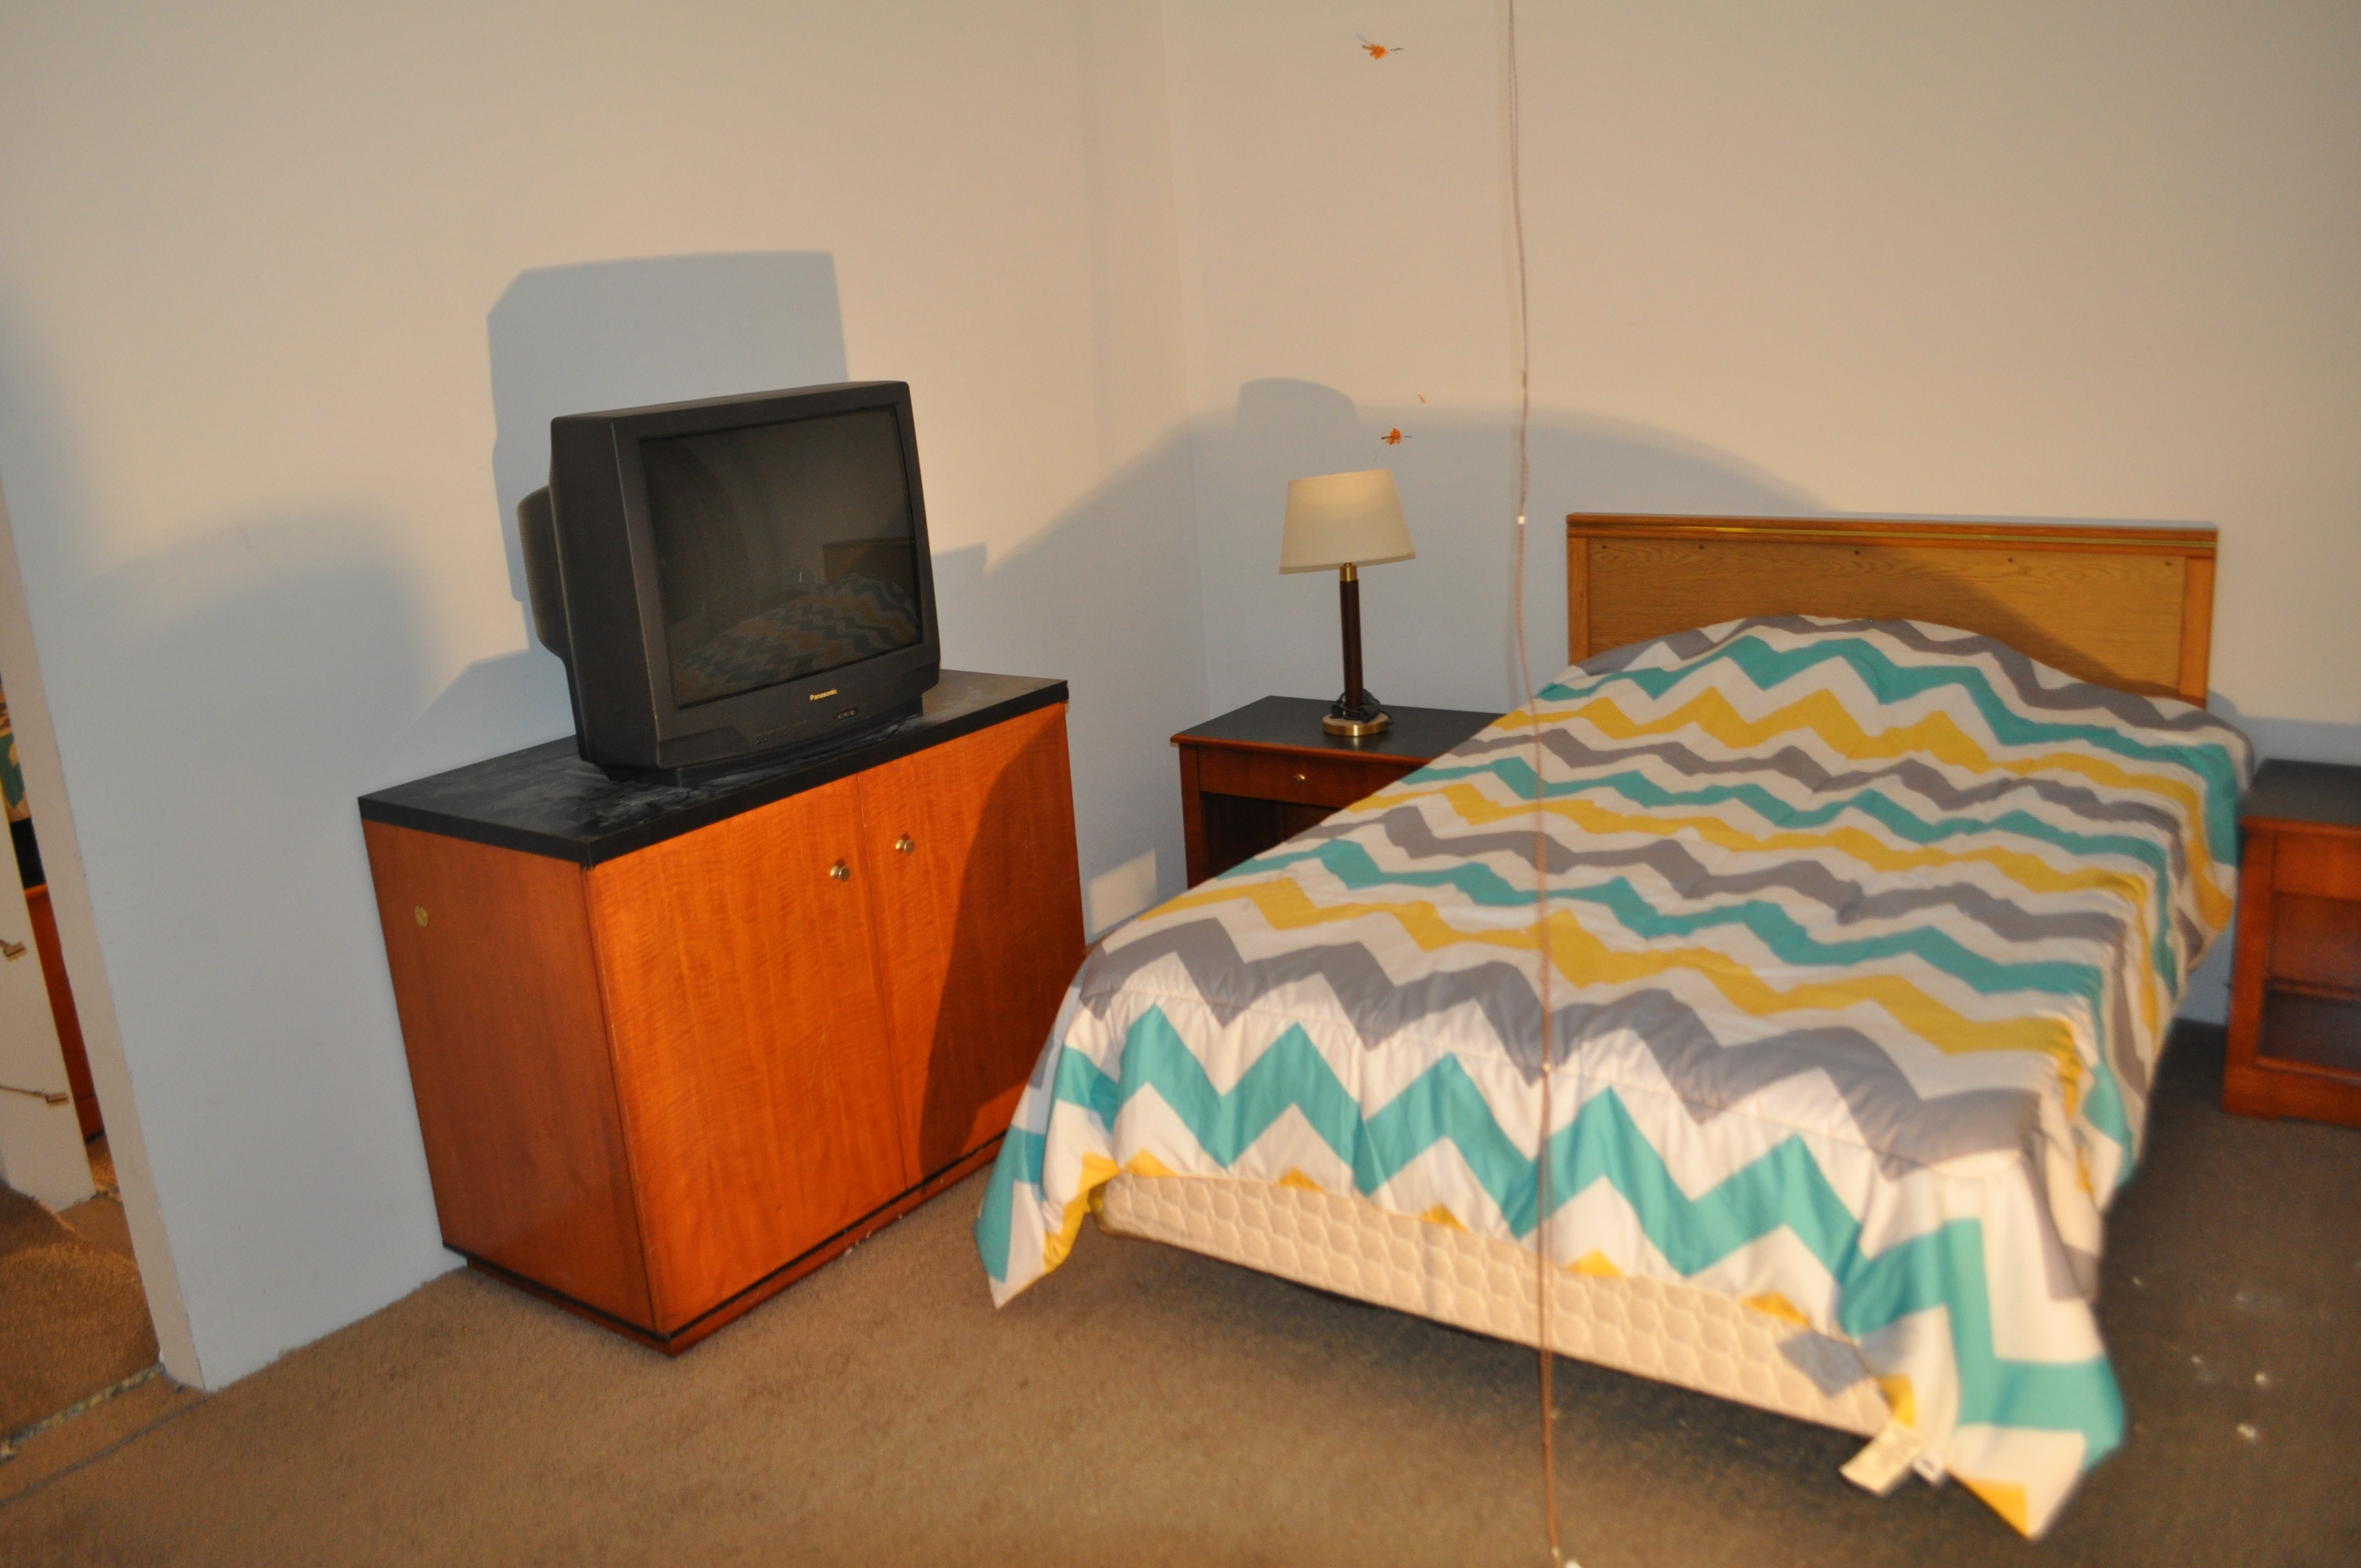
\includegraphics[width=3in]{0_Images/Furniture/1StoryMaster.jpg}} &
		\subfloat[Two Story Master]{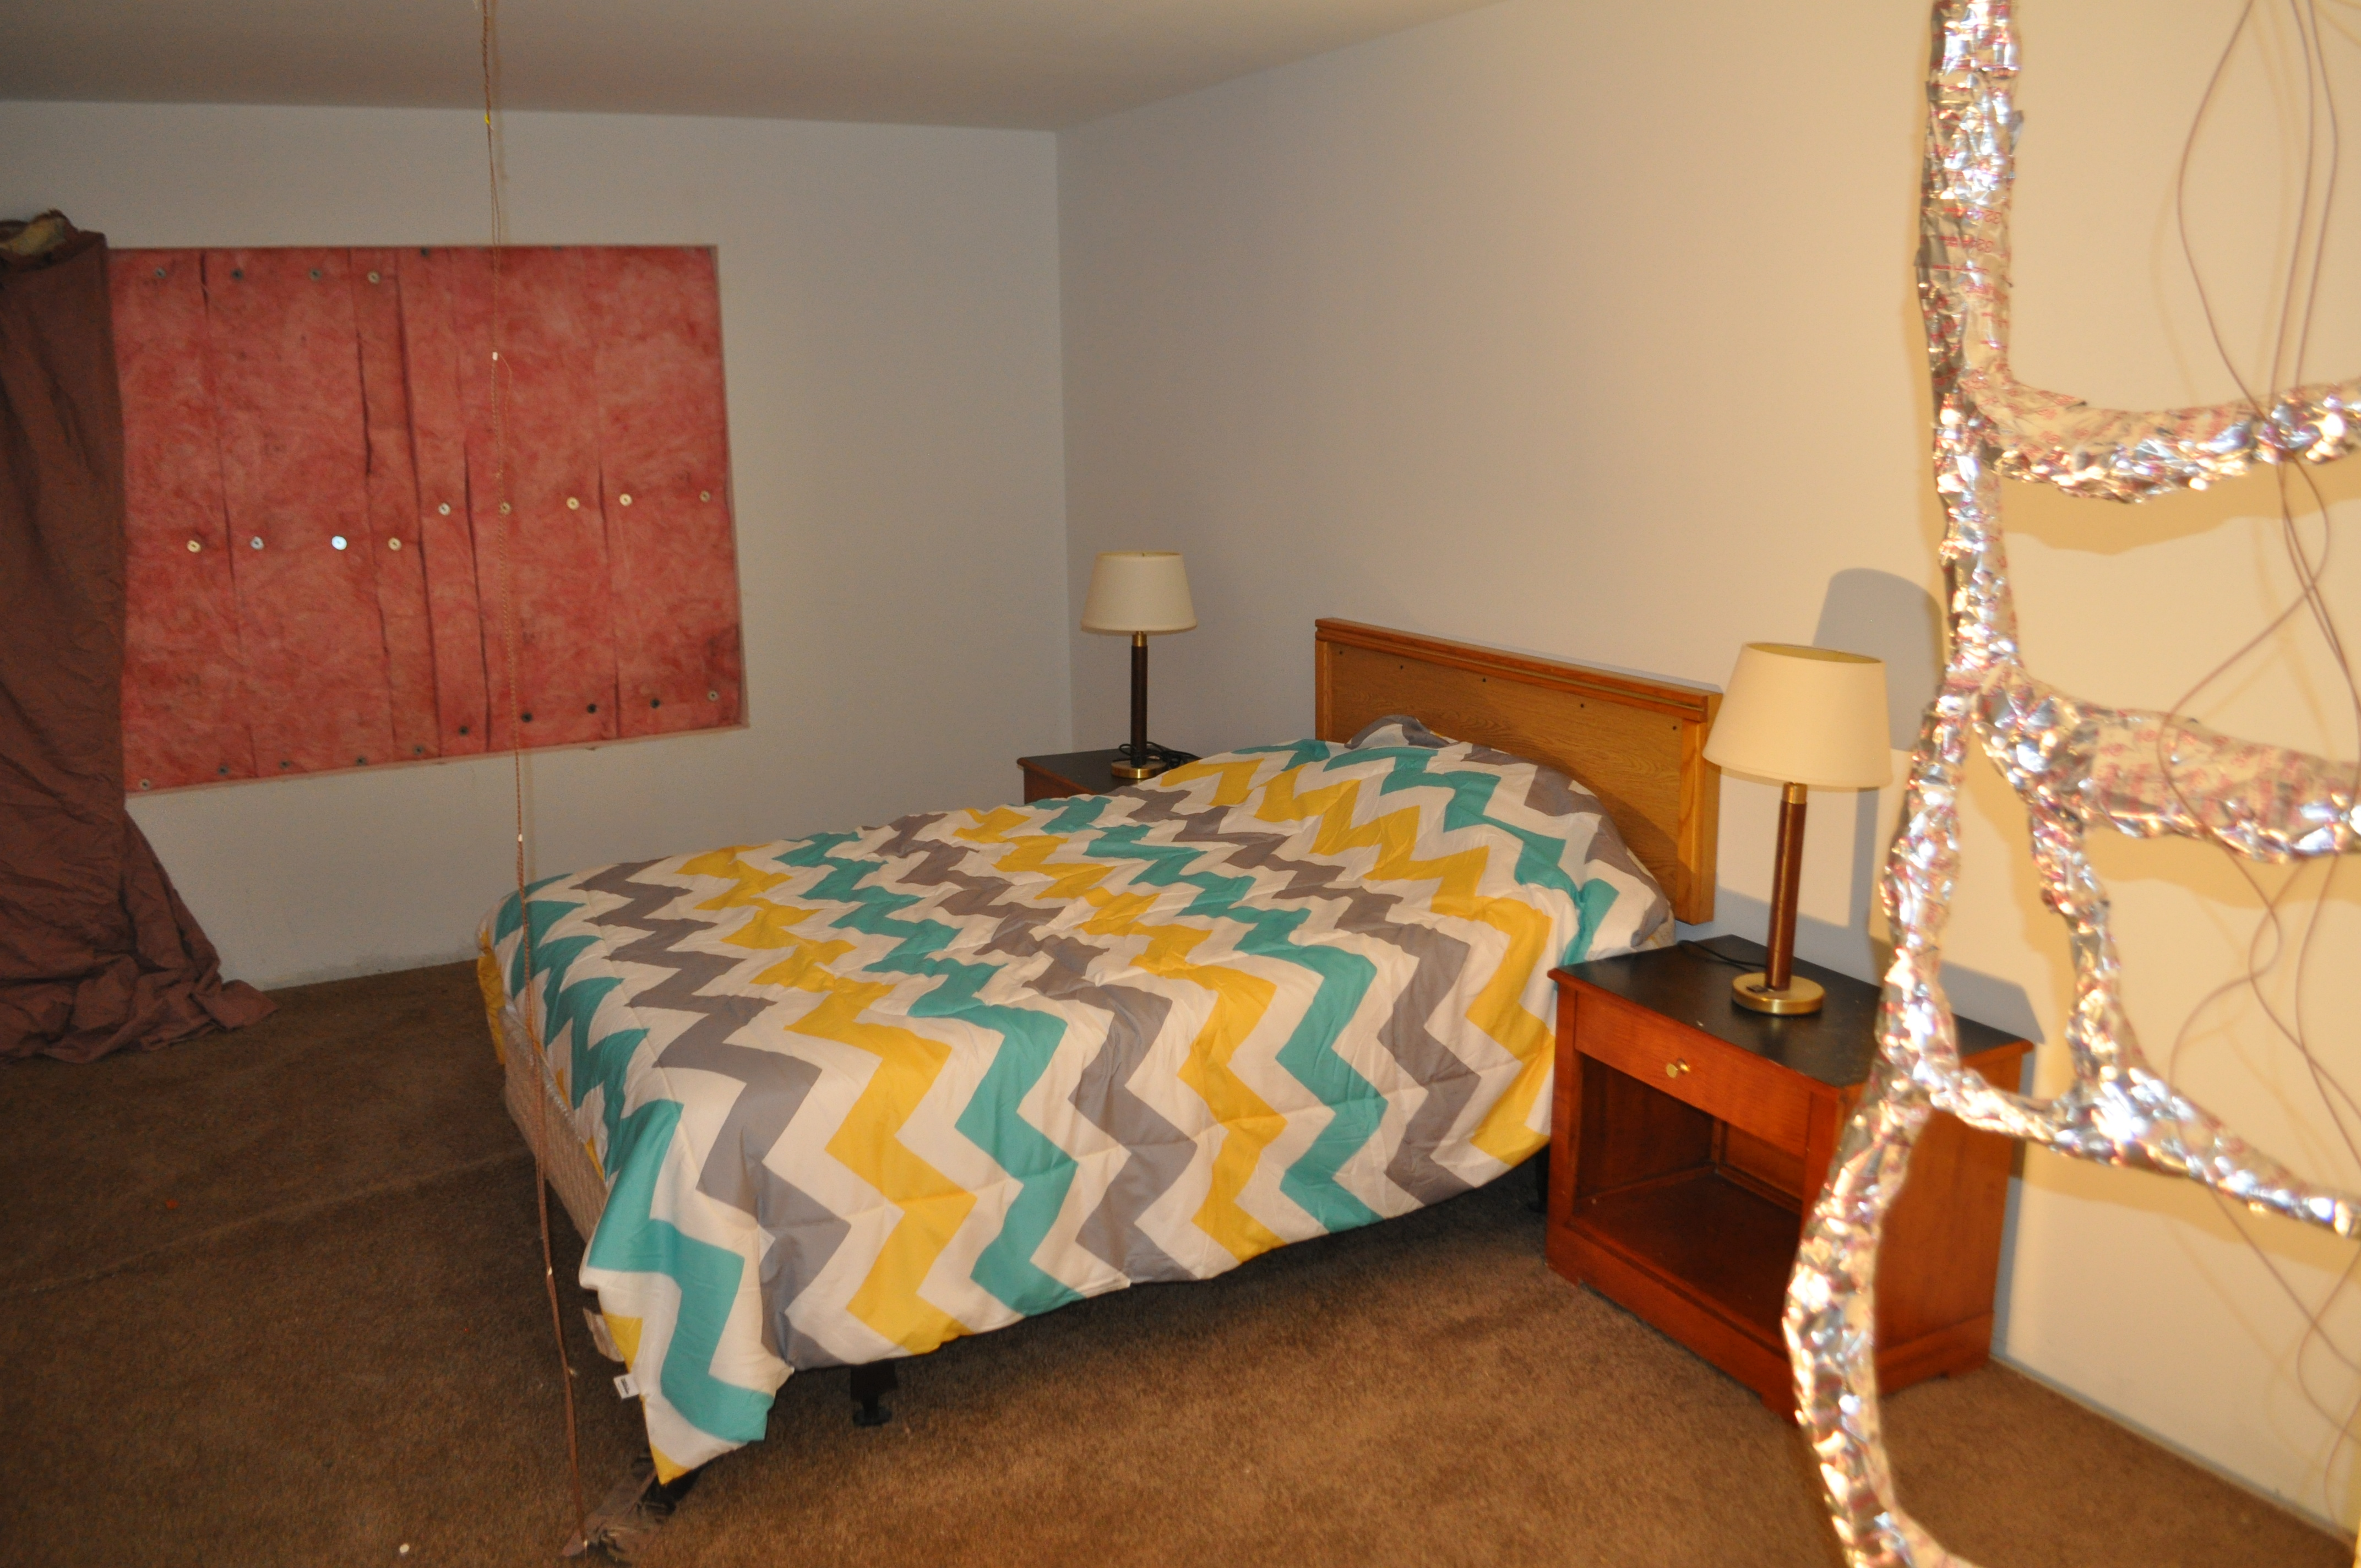
\includegraphics[width=3in]{0_Images/Furniture/2StoryMaster.jpg}} \\
	\end{tabular}
	\caption{Master Bedroom Furniture}
	\label{fig:MasterBedrooms}
\end{figure}

The remainder of the bedrooms in both houses were furnished with the same bed, television stand, television and flooring compliment as well as a light brown dresser, and headboard. For fires located in the bedrooms an additional mattress was added to the bed to extend burn duration. Figure \ref{fig:Bedrooms} shows the furniture setup for both the single story and two story bedrooms. 

\begin{figure}[H]
	\centering
	\begin{tabular}[c]{c c}
		\subfloat[Single Story Bedroom 2]{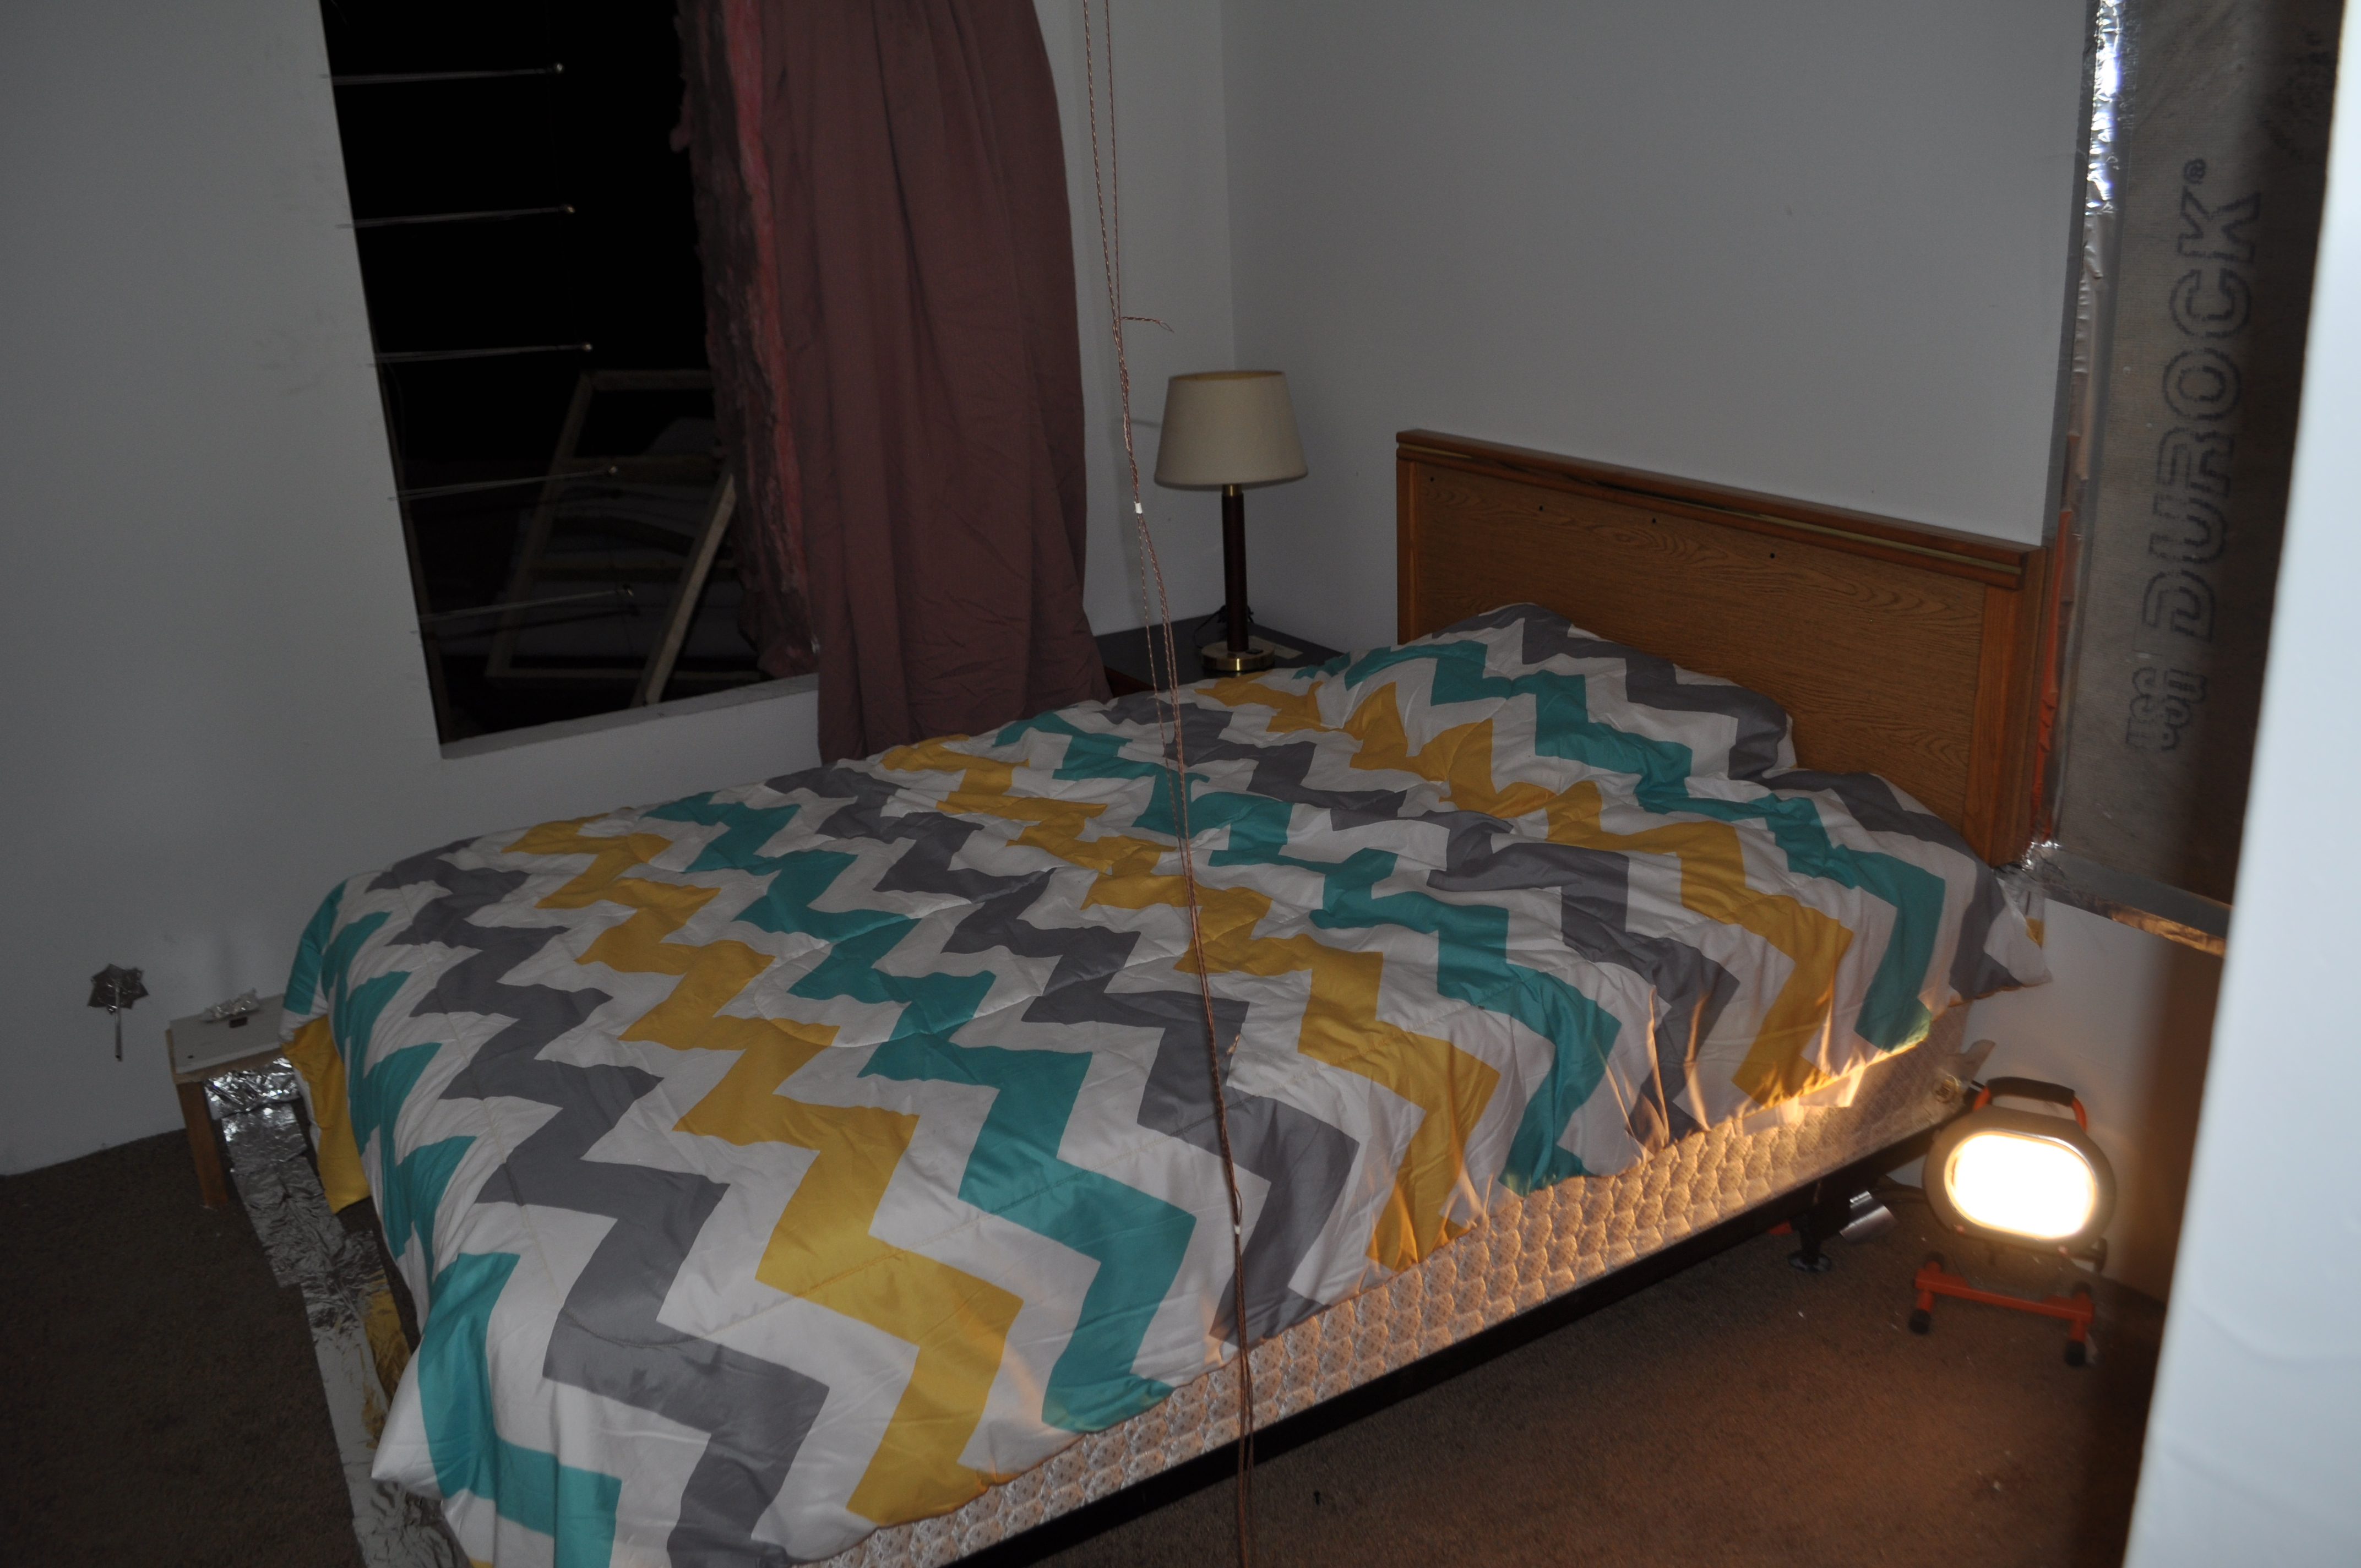
\includegraphics[width=3in]{0_Images/Furniture/1StoryBed2.jpg}} &
		\subfloat[Single Story Bedroom 3]{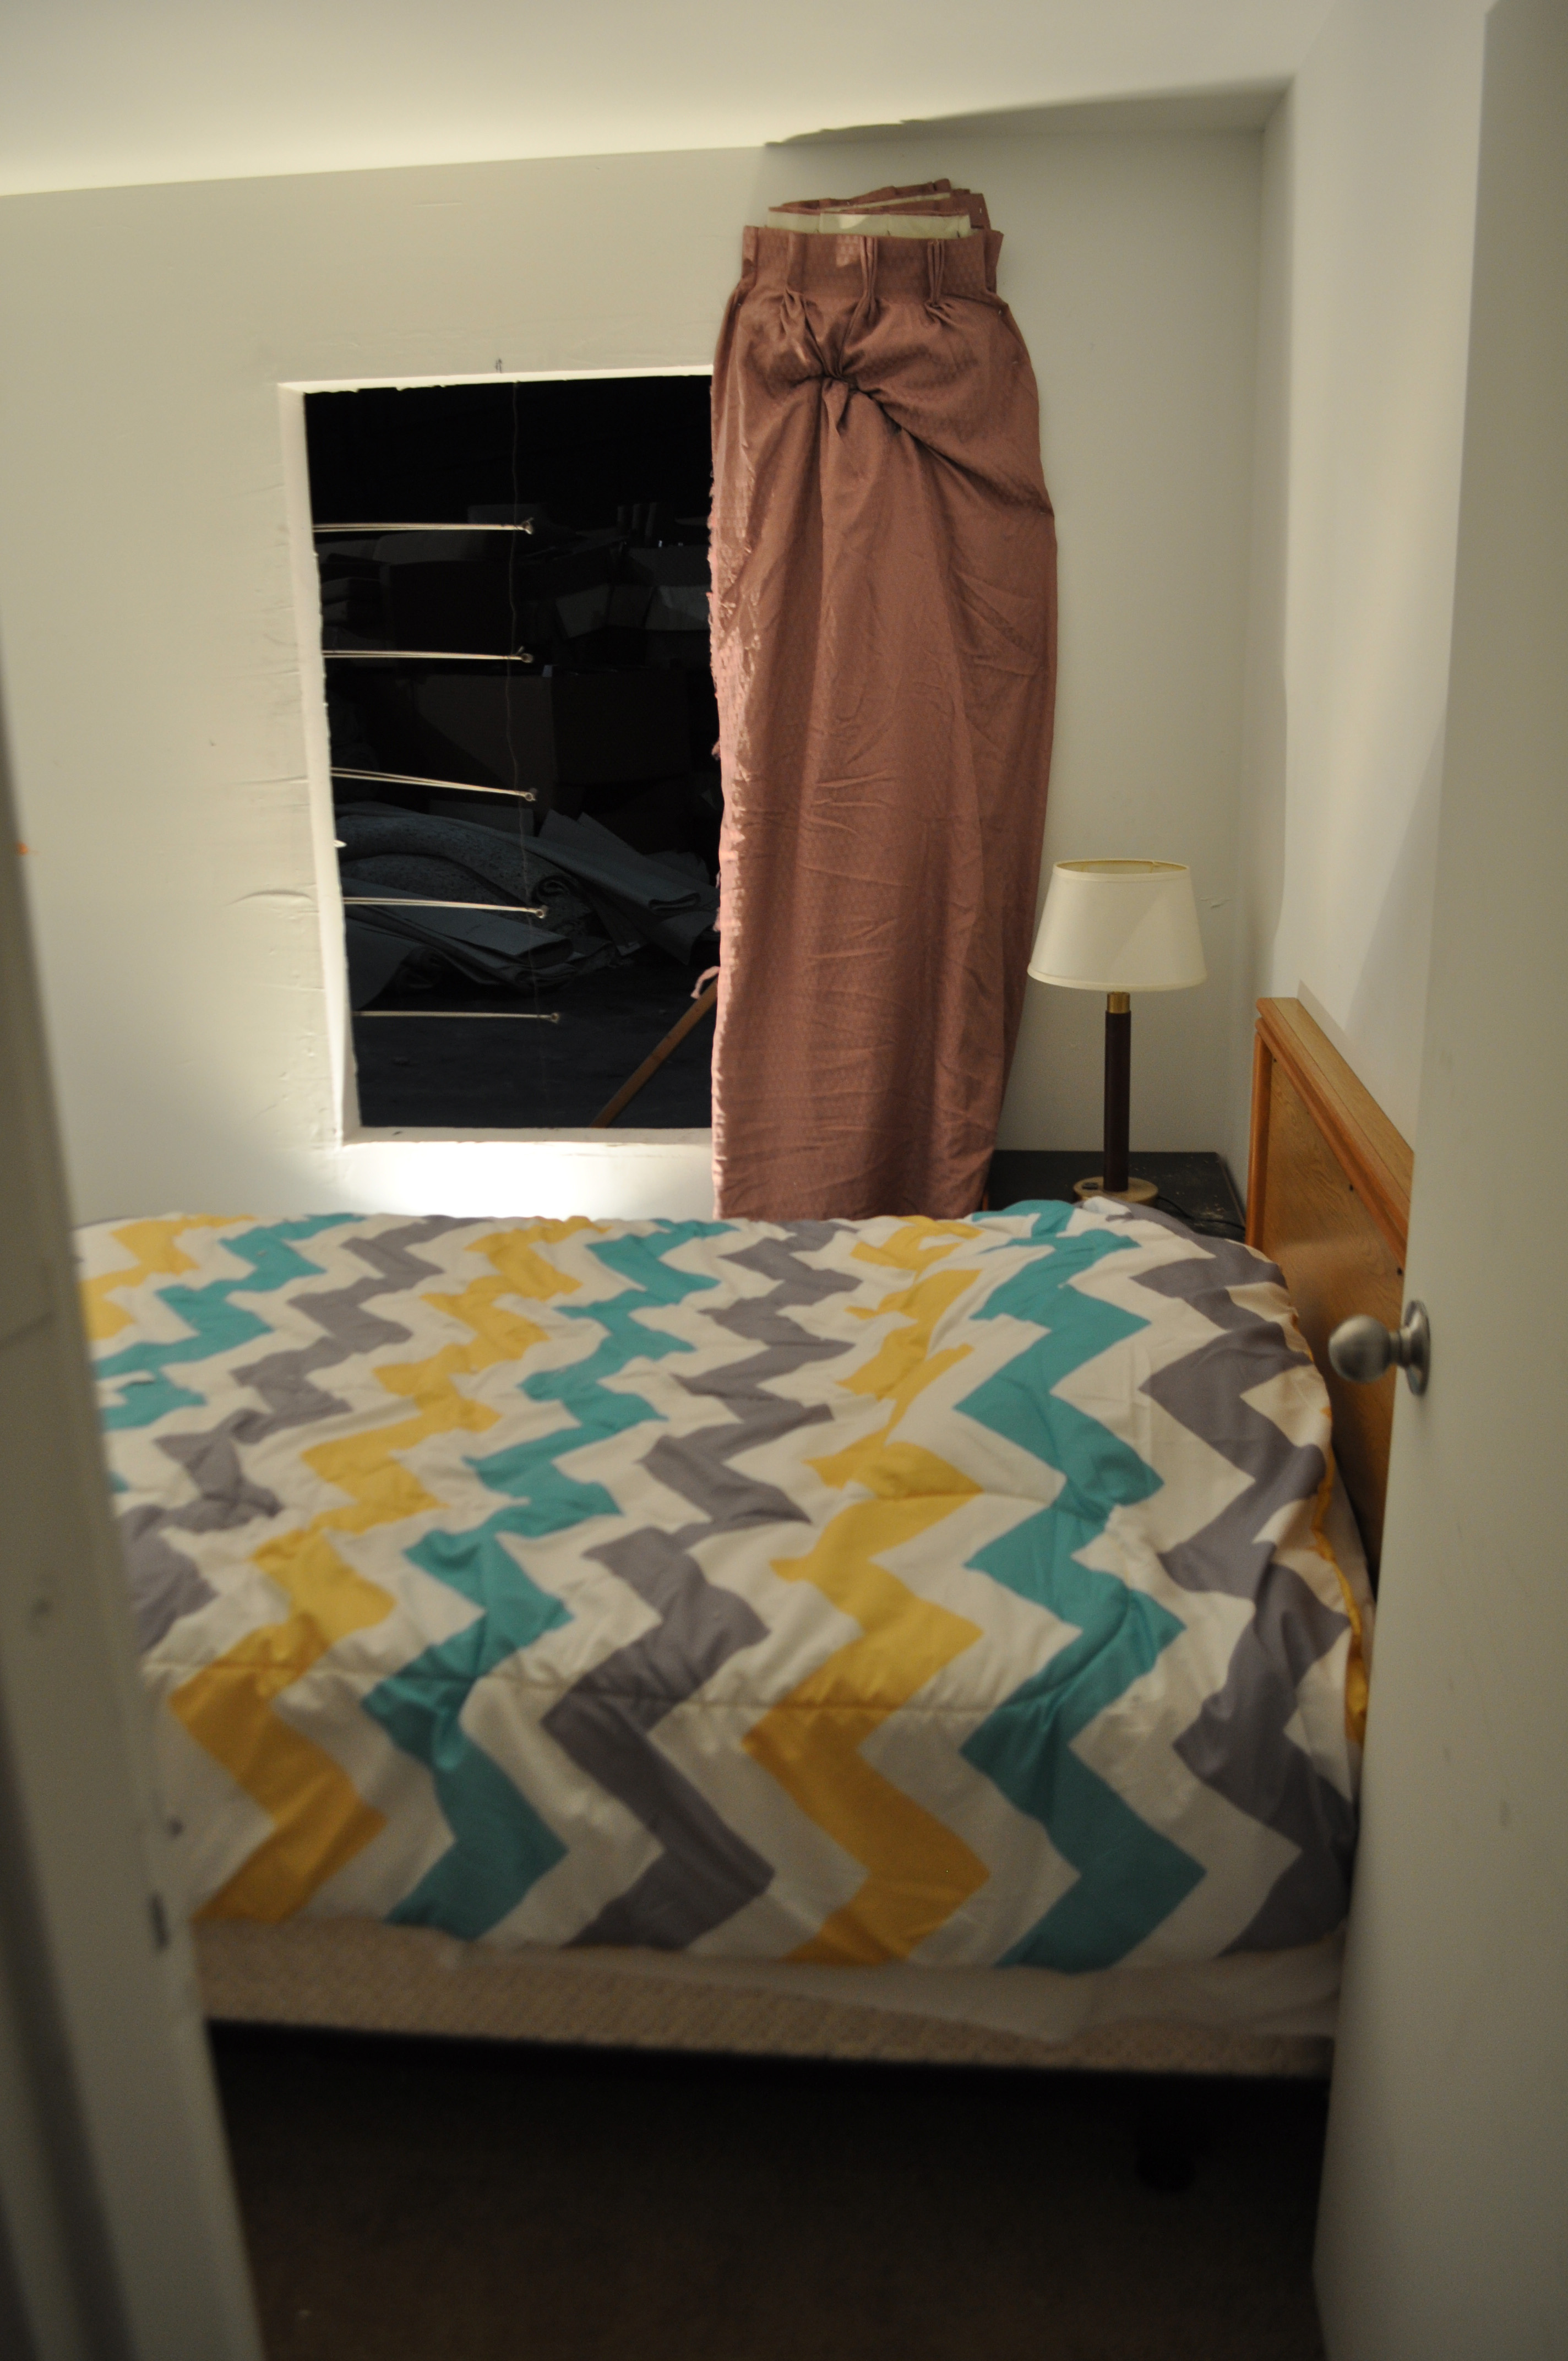
\includegraphics[width=1.5in]{0_Images/Furniture/1StoryBed3.jpg}} \\
		\subfloat[Two Story Bedroom 2]{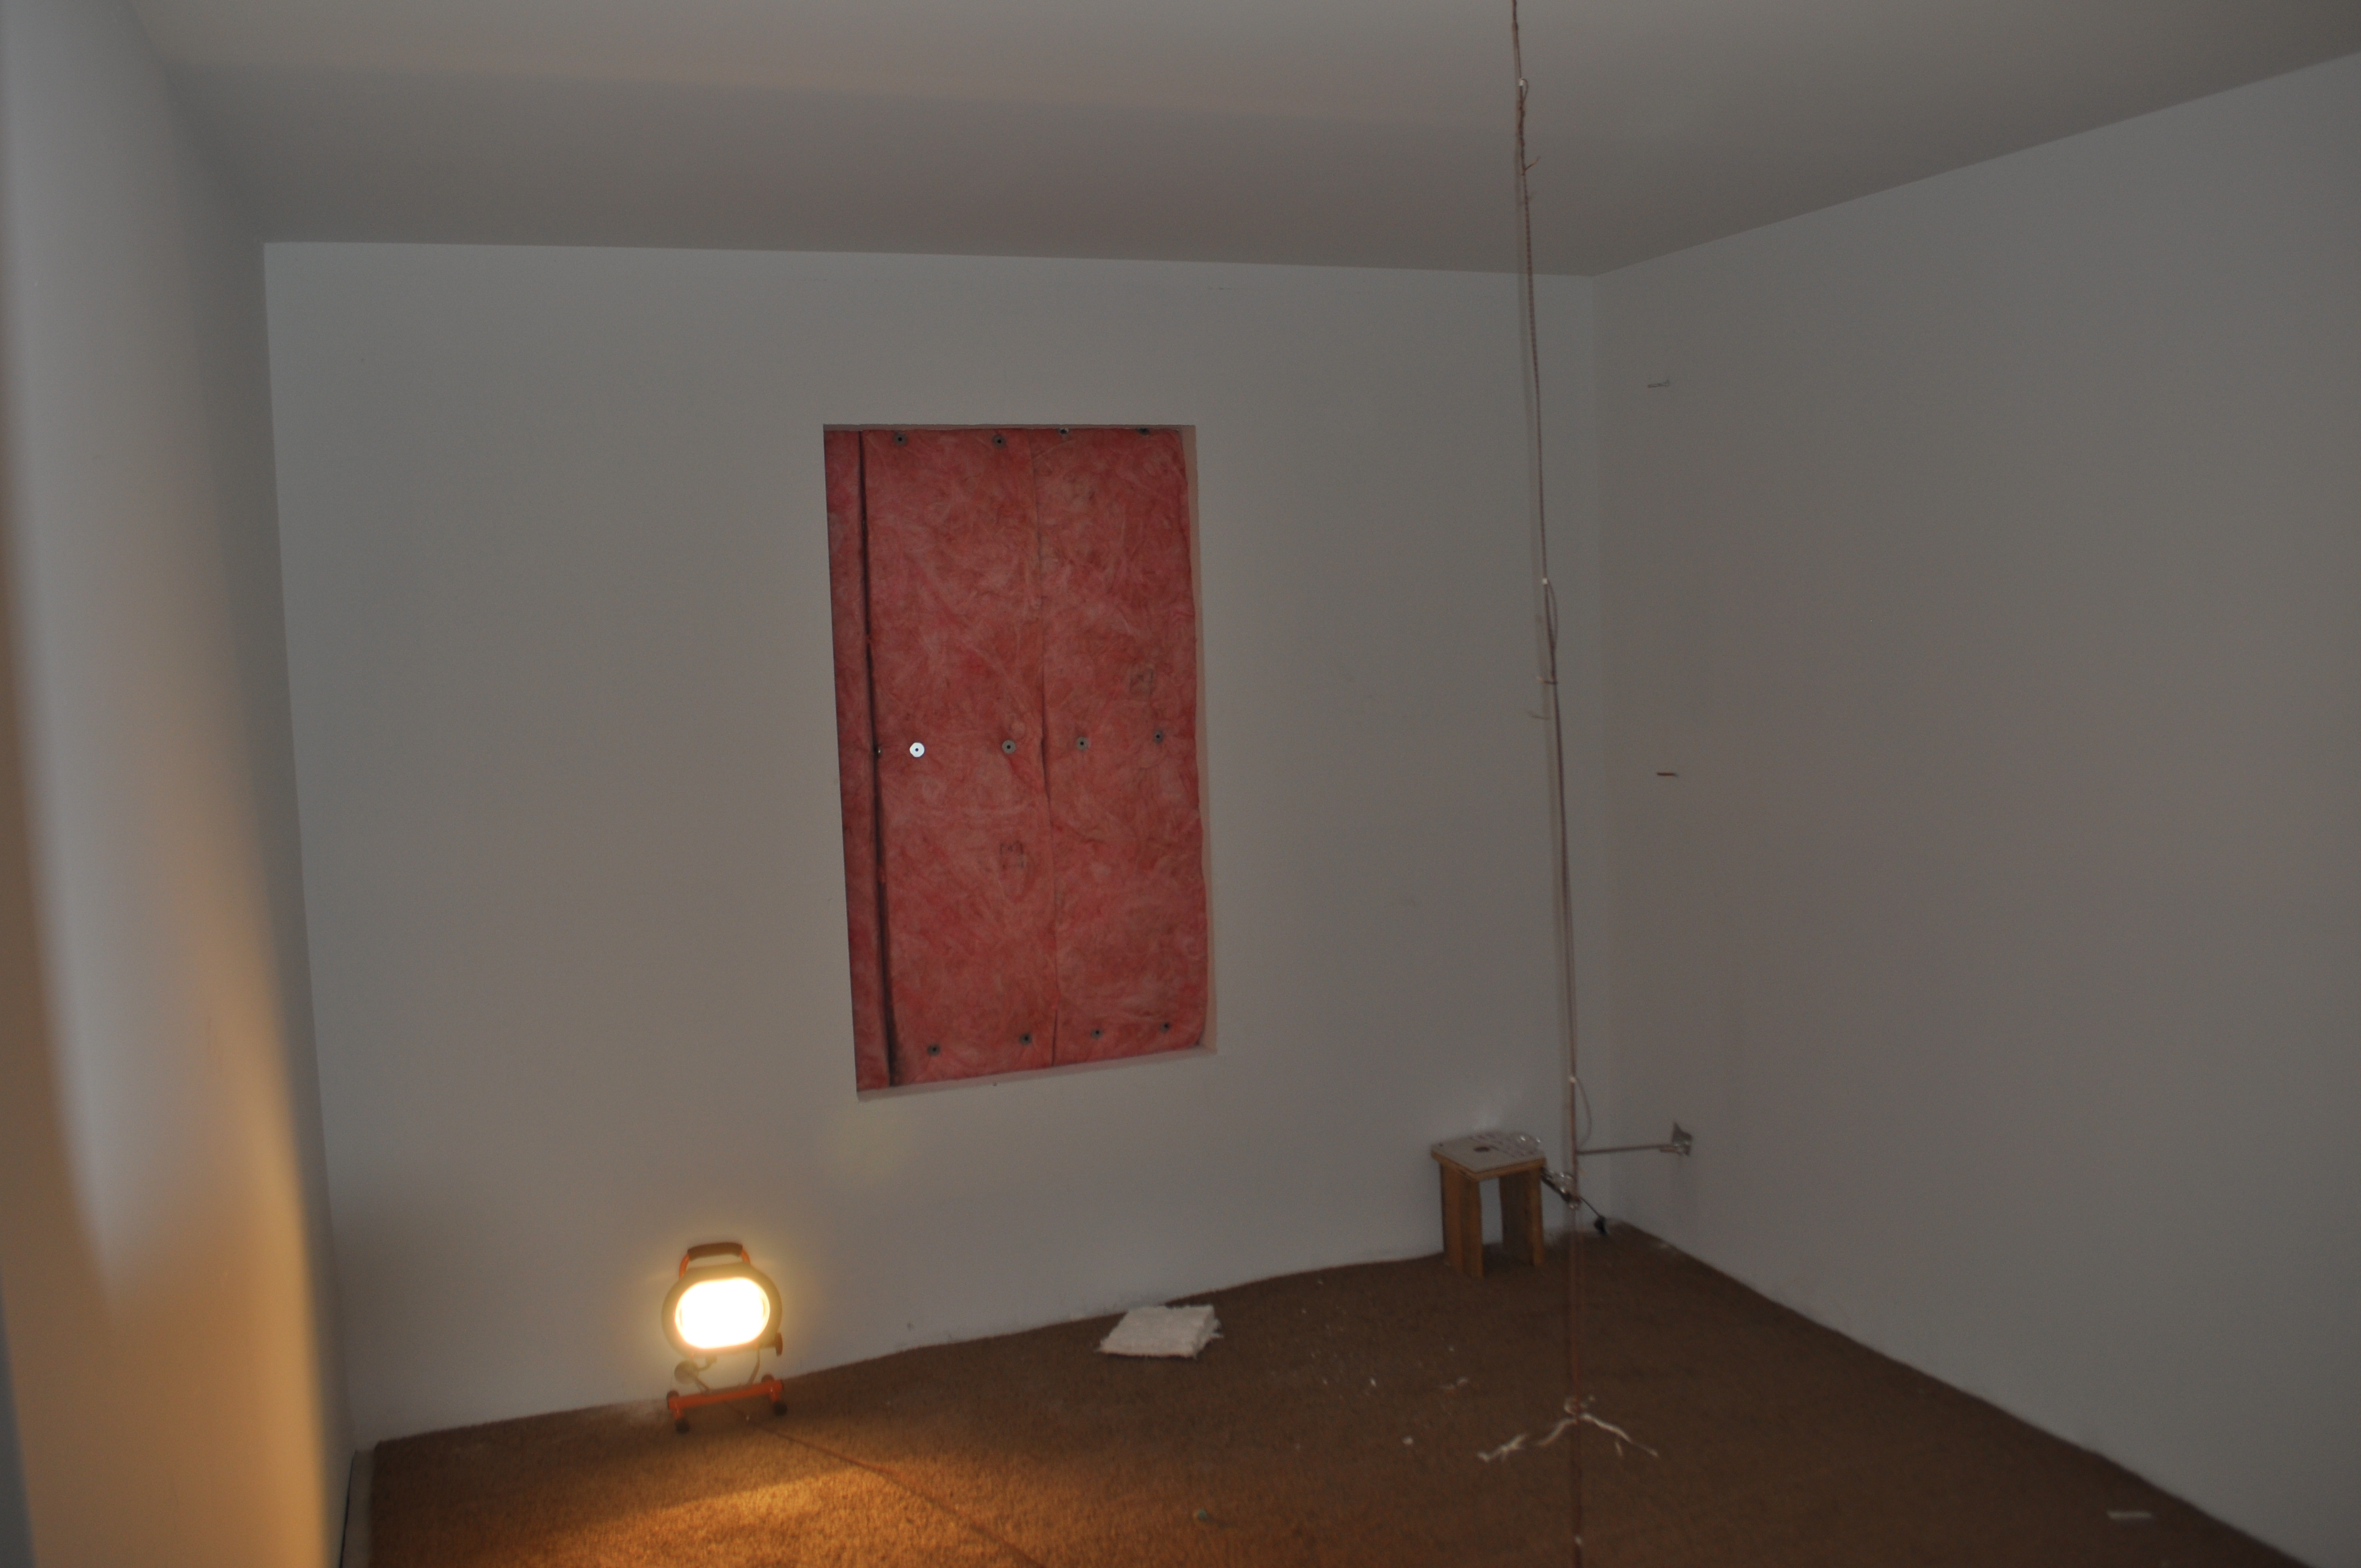
\includegraphics[width=3in]{0_Images/Furniture/2StoryBed2.jpg}} &
		\subfloat[Two Story Bedroom 3]{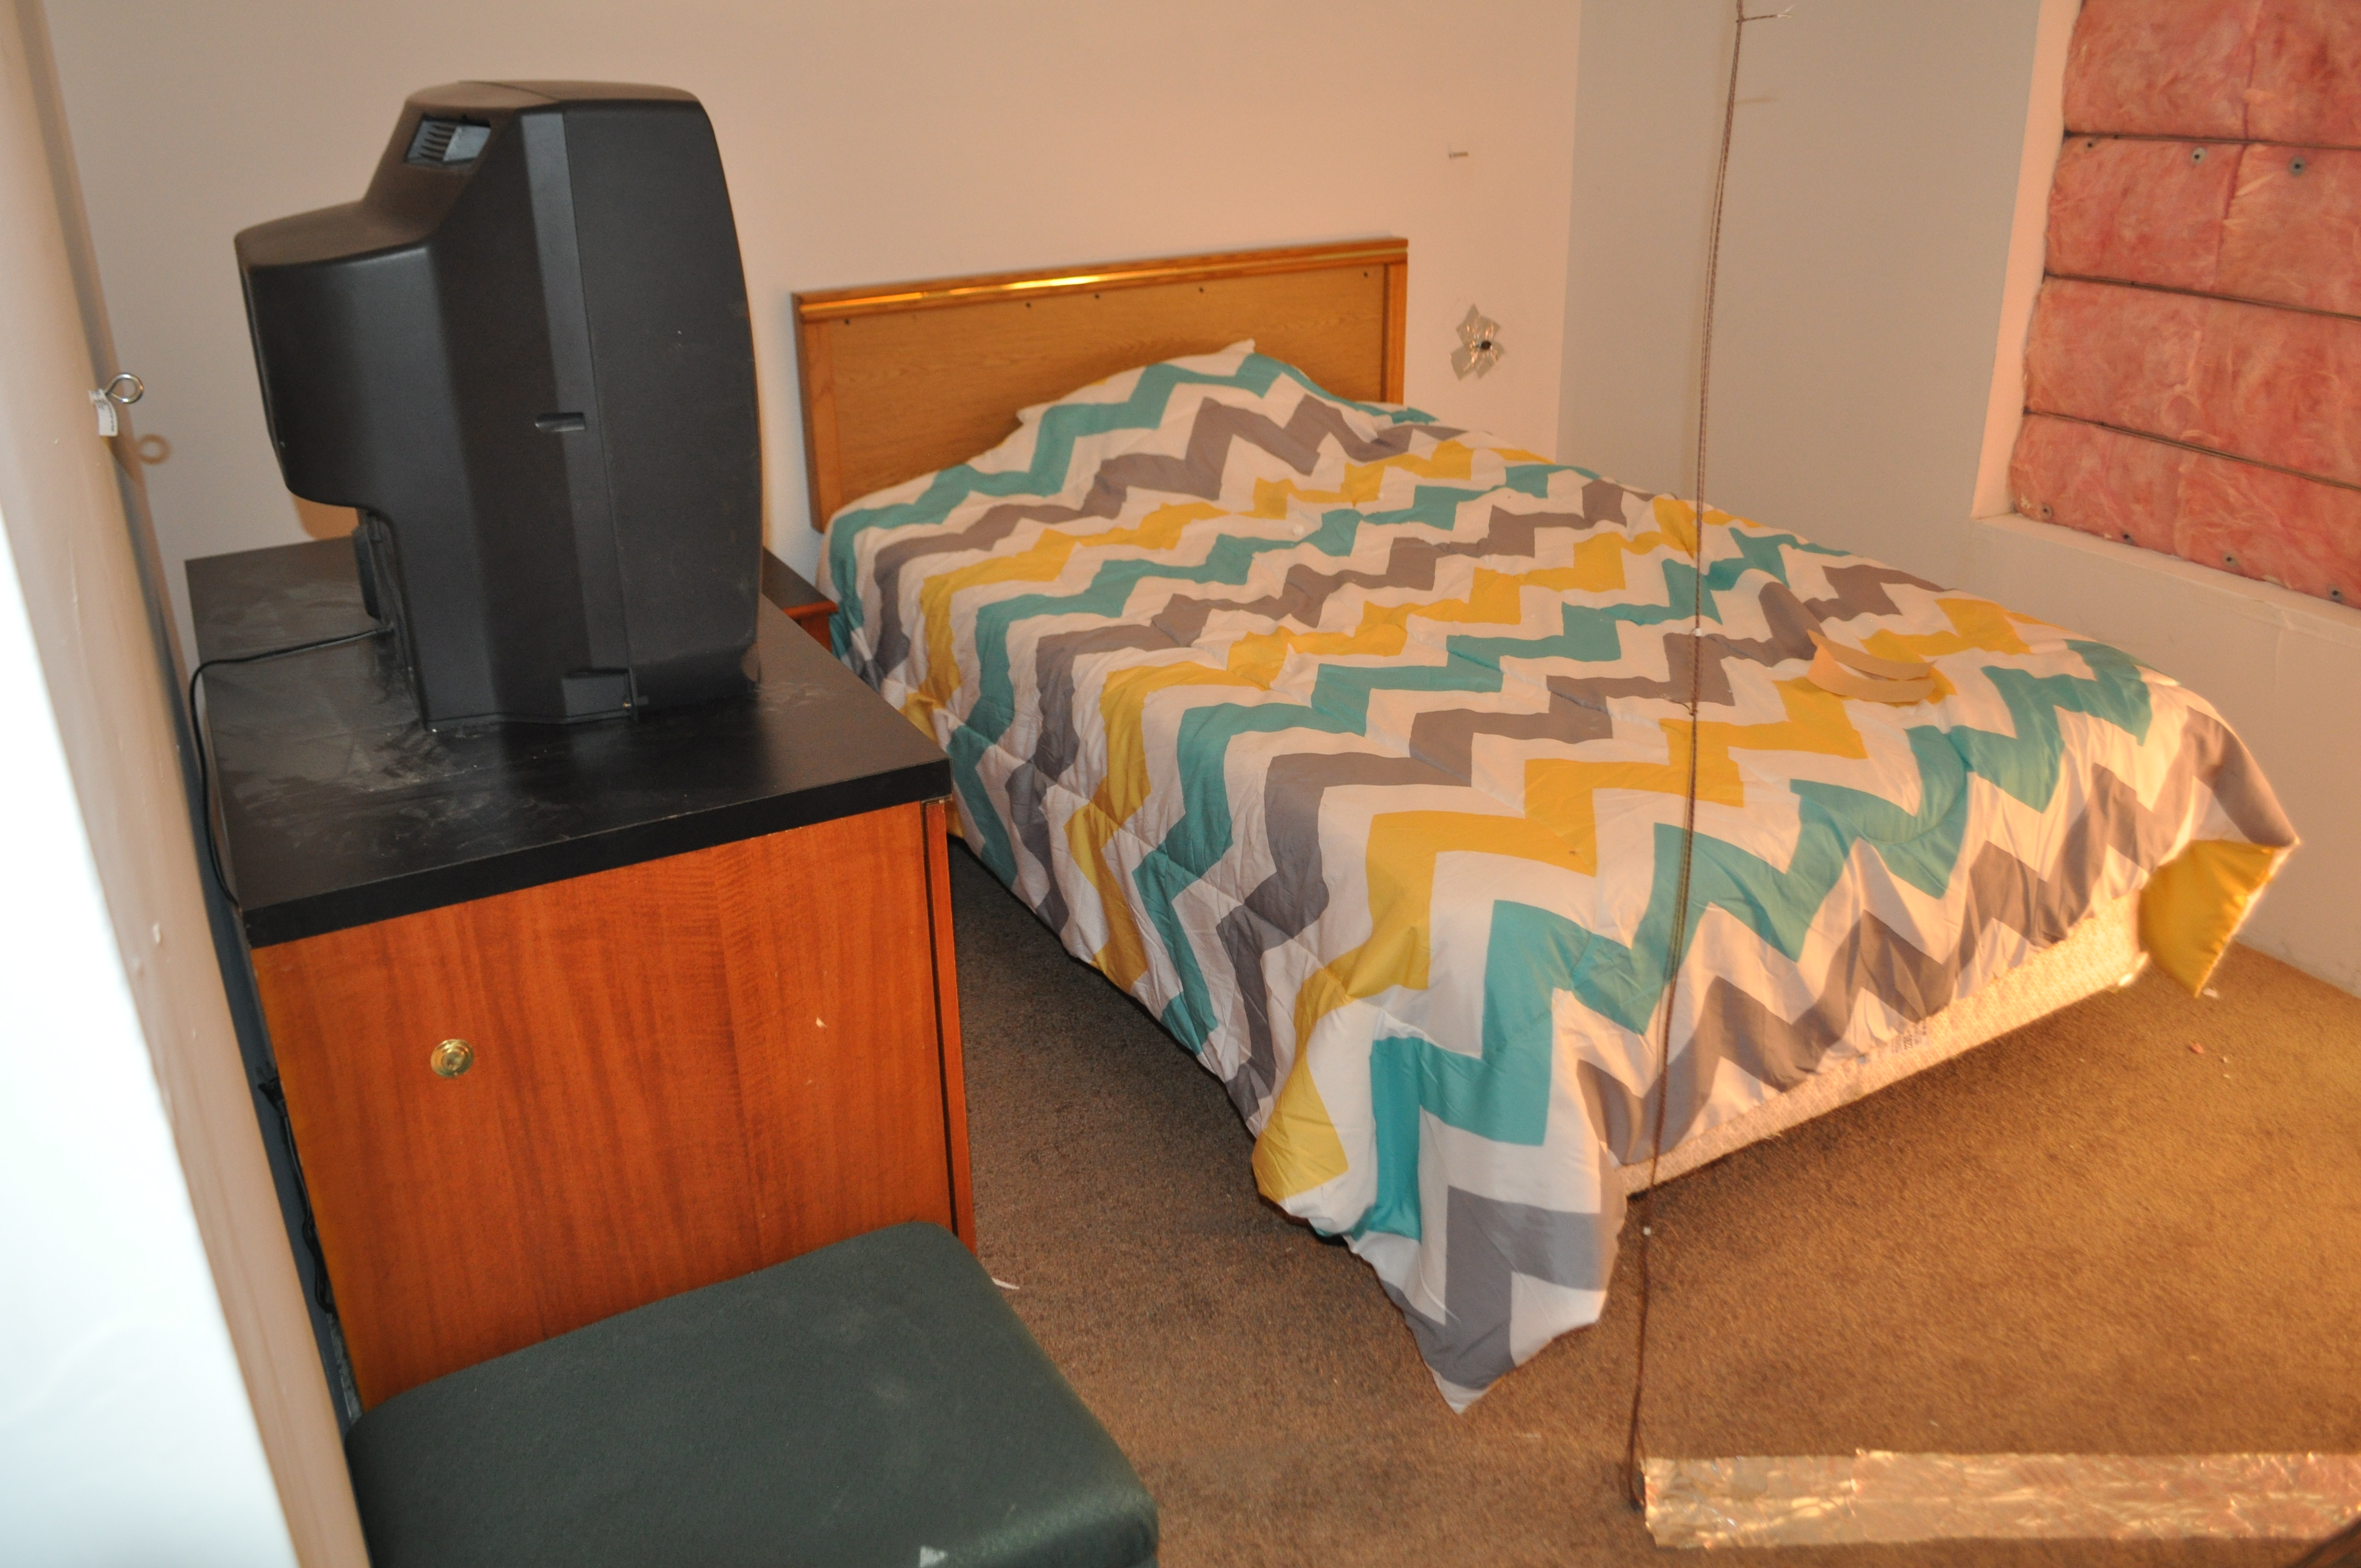
\includegraphics[width=3in]{0_Images/Furniture/2StoryBed3.jpg}} \\
	\end{tabular}
	\centering	
	\subfloat[Two Story Bedroom 4]{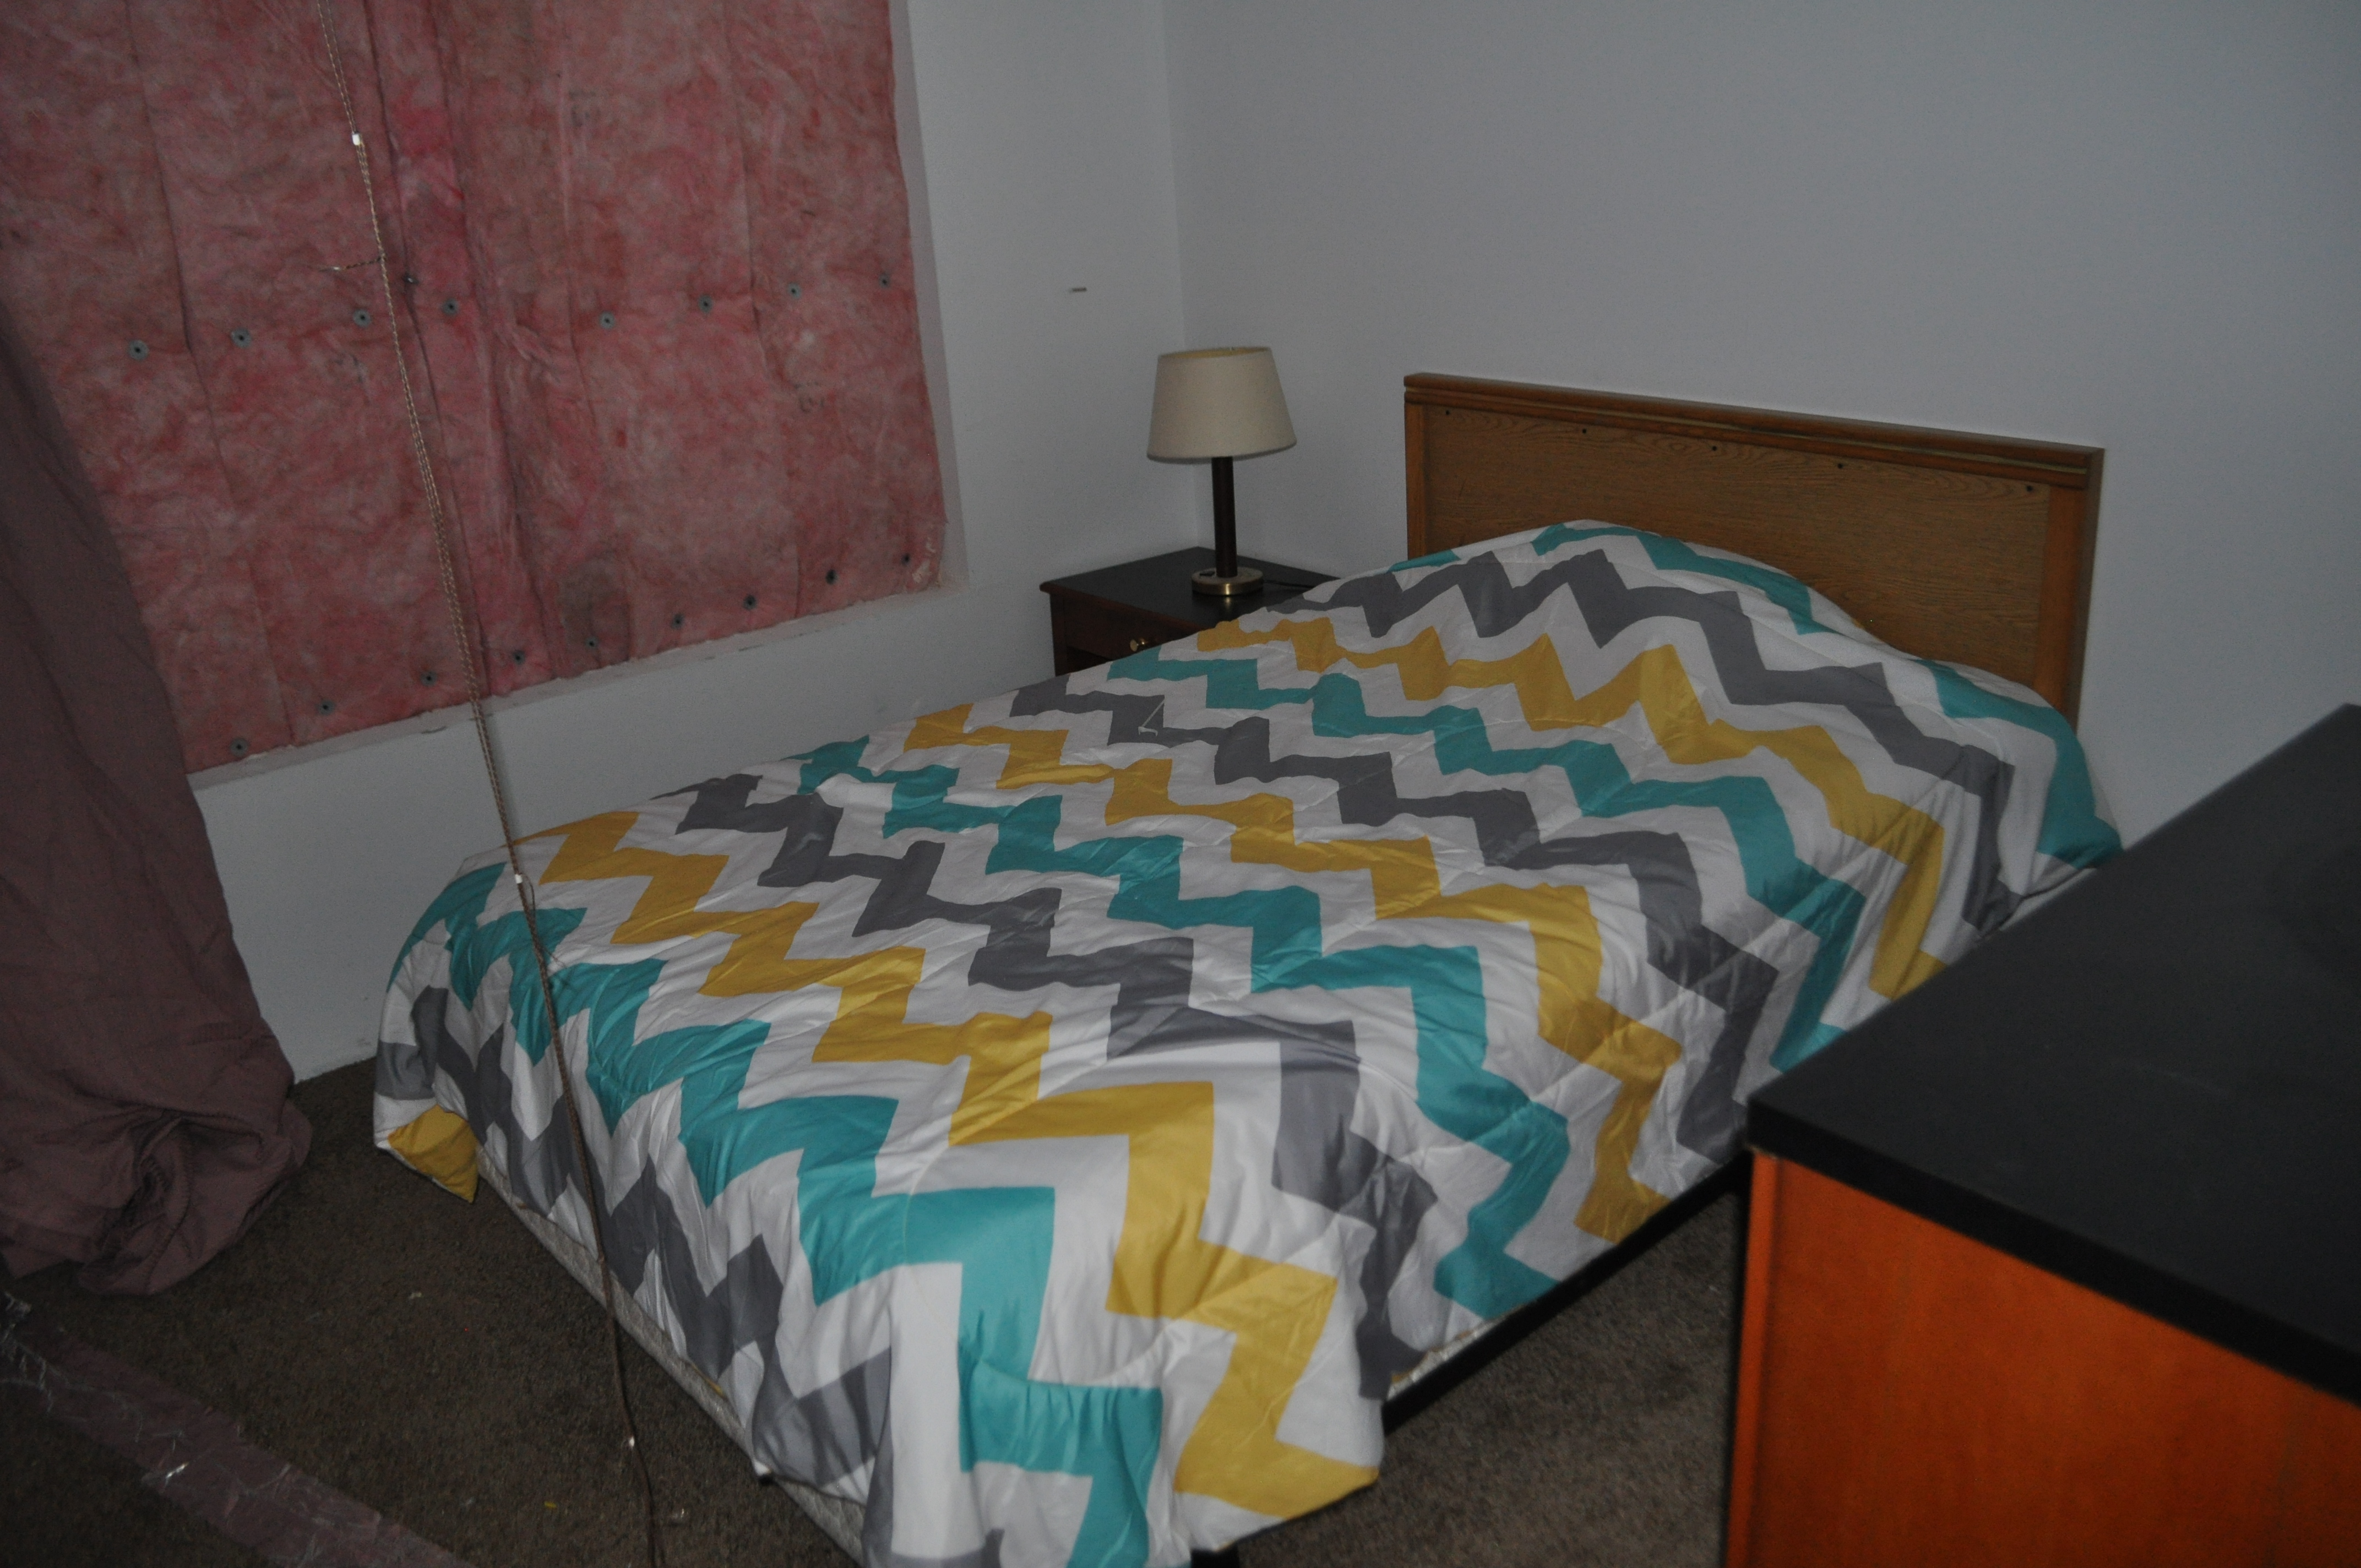
\includegraphics[width=3in]{0_Images/Furniture/2StoryBed4.jpg}} \\
	\caption{Bedroom Furniture}
	\label{fig:Bedrooms}
\end{figure}

The dining room of both houses was furnished with two solid wood tables put together as a single table and six kitchen chairs. The tables were centered in the space with the chairs surrounding them. Figure \ref{fig:Dinning} shows the furniture setup for both the single story and two story dining rooms. 

\begin{figure}[H]
	\centering
	\begin{tabular}[c]{c c}
		\subfloat[Single Story Dining]{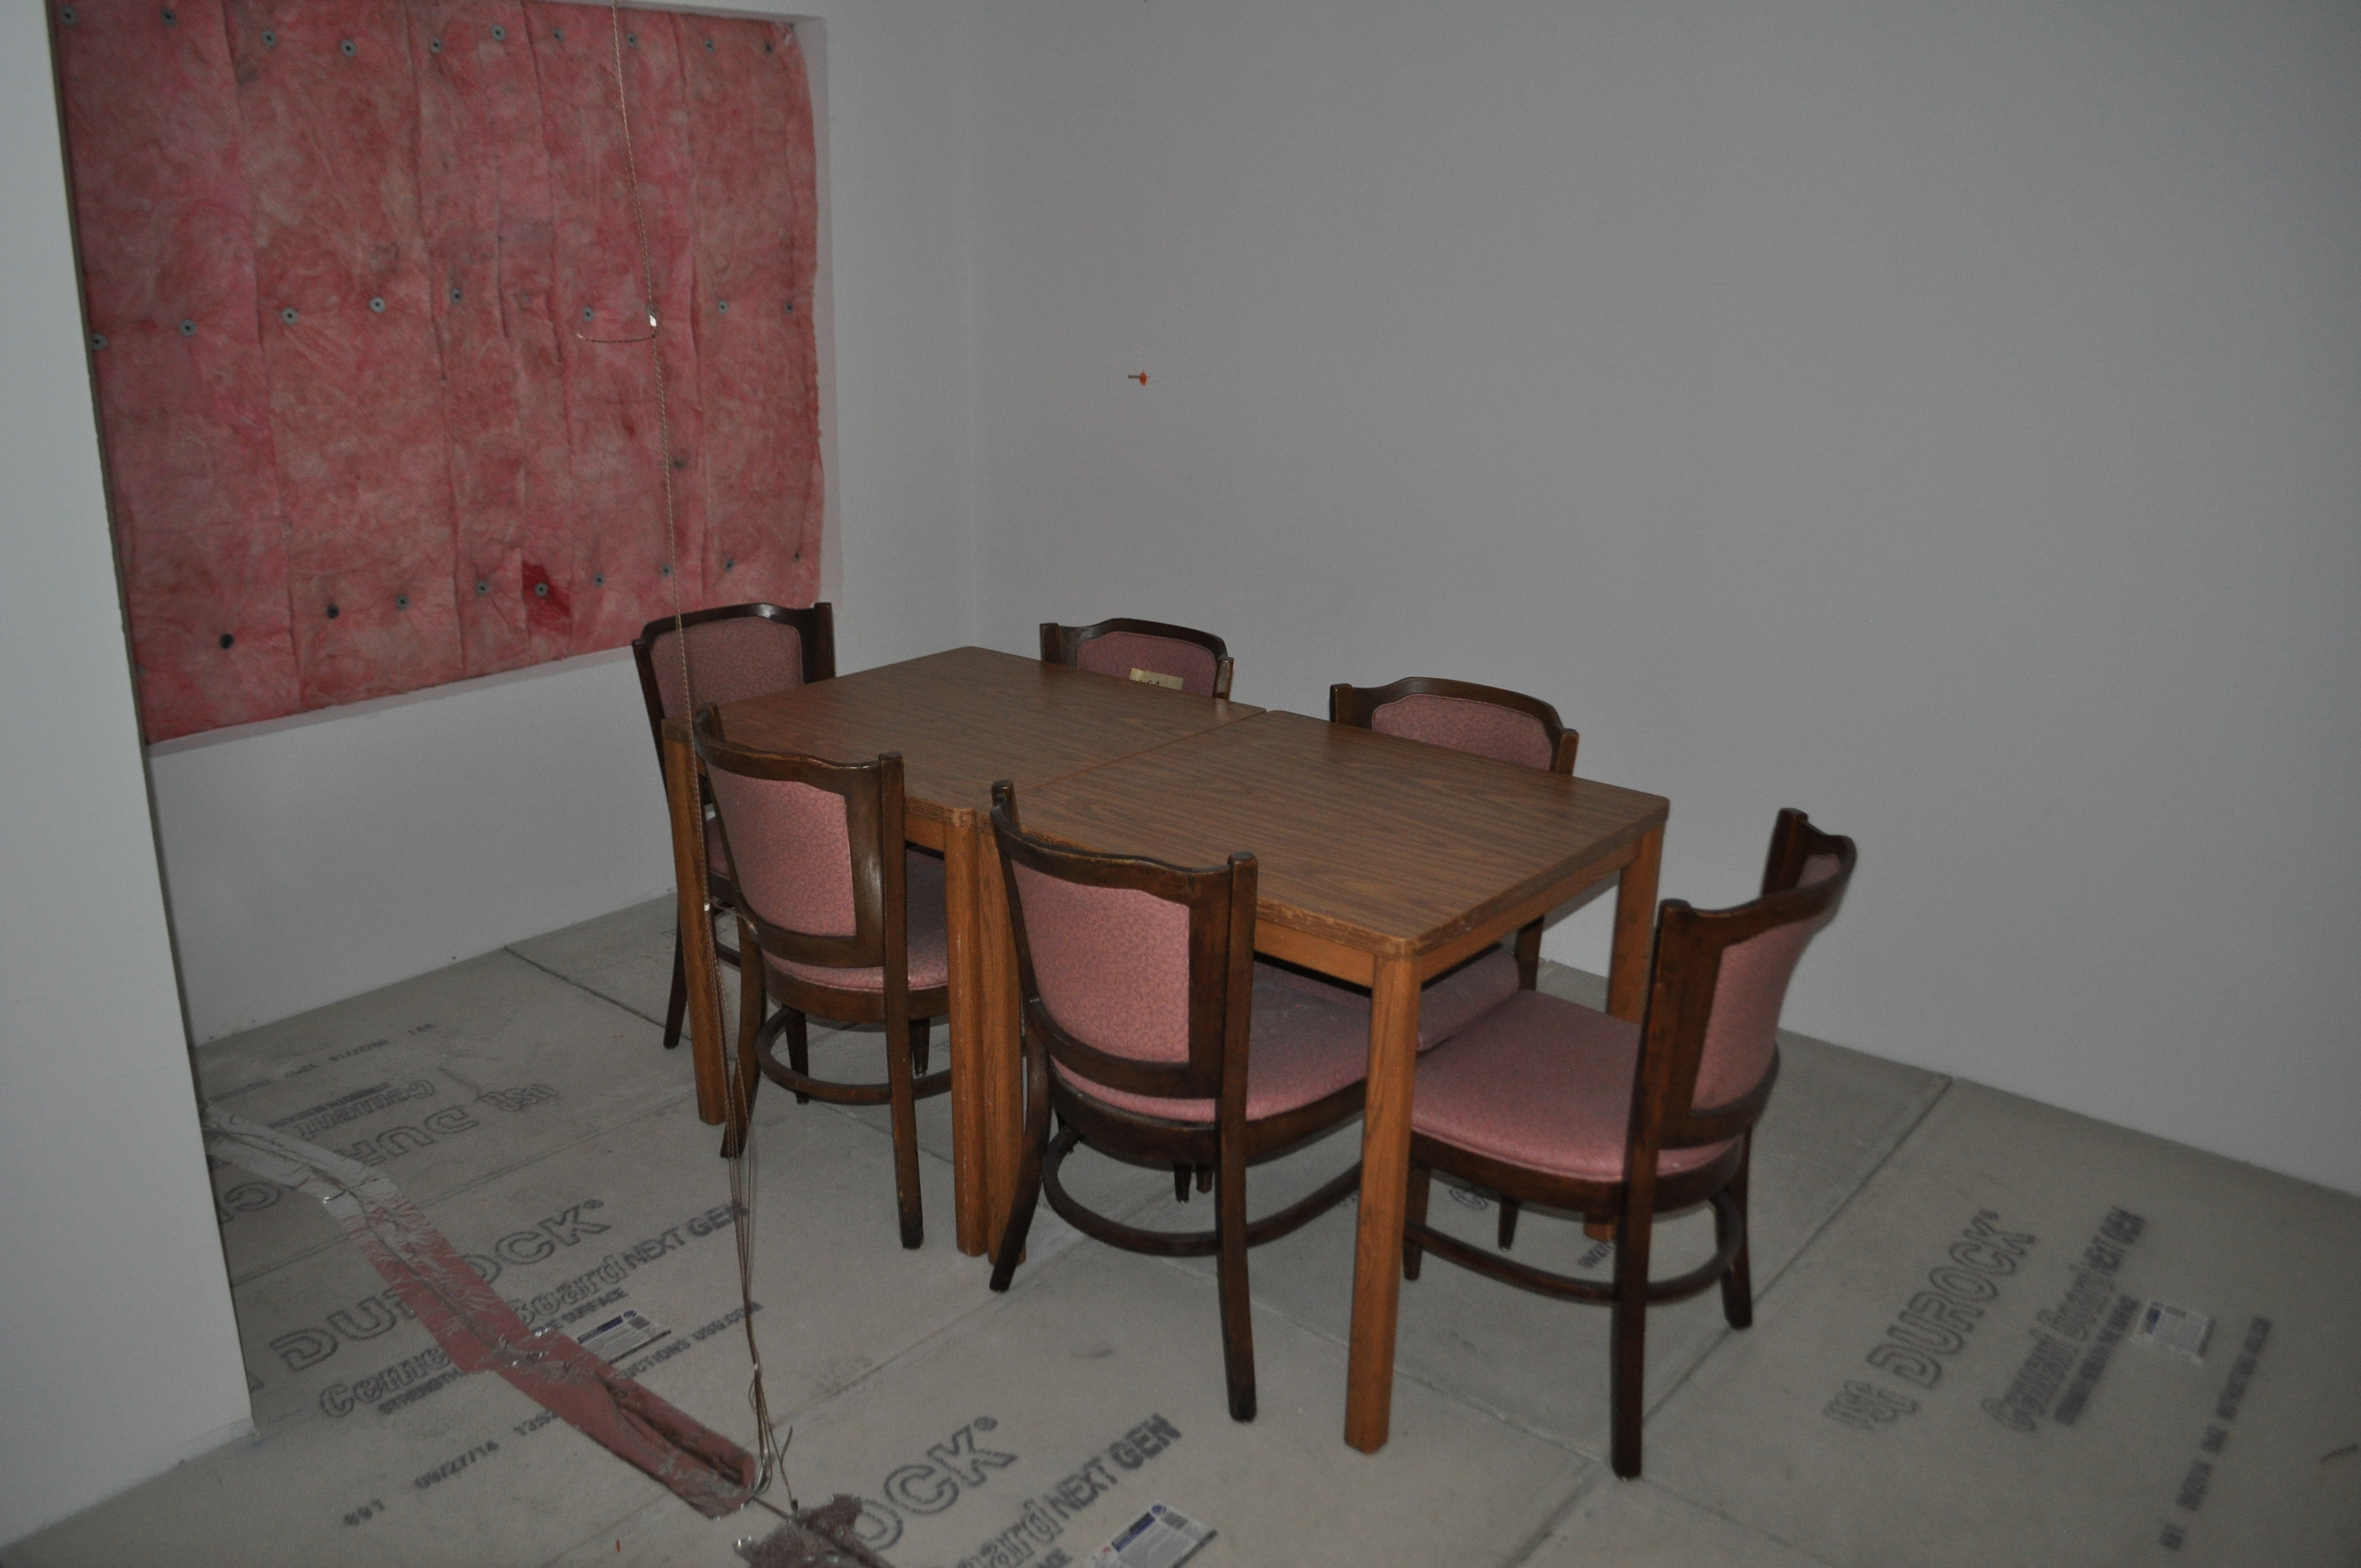
\includegraphics[width=3in]{0_Images/Furniture/1StoryDining.jpg}} &
		\subfloat[Two Story Dining]{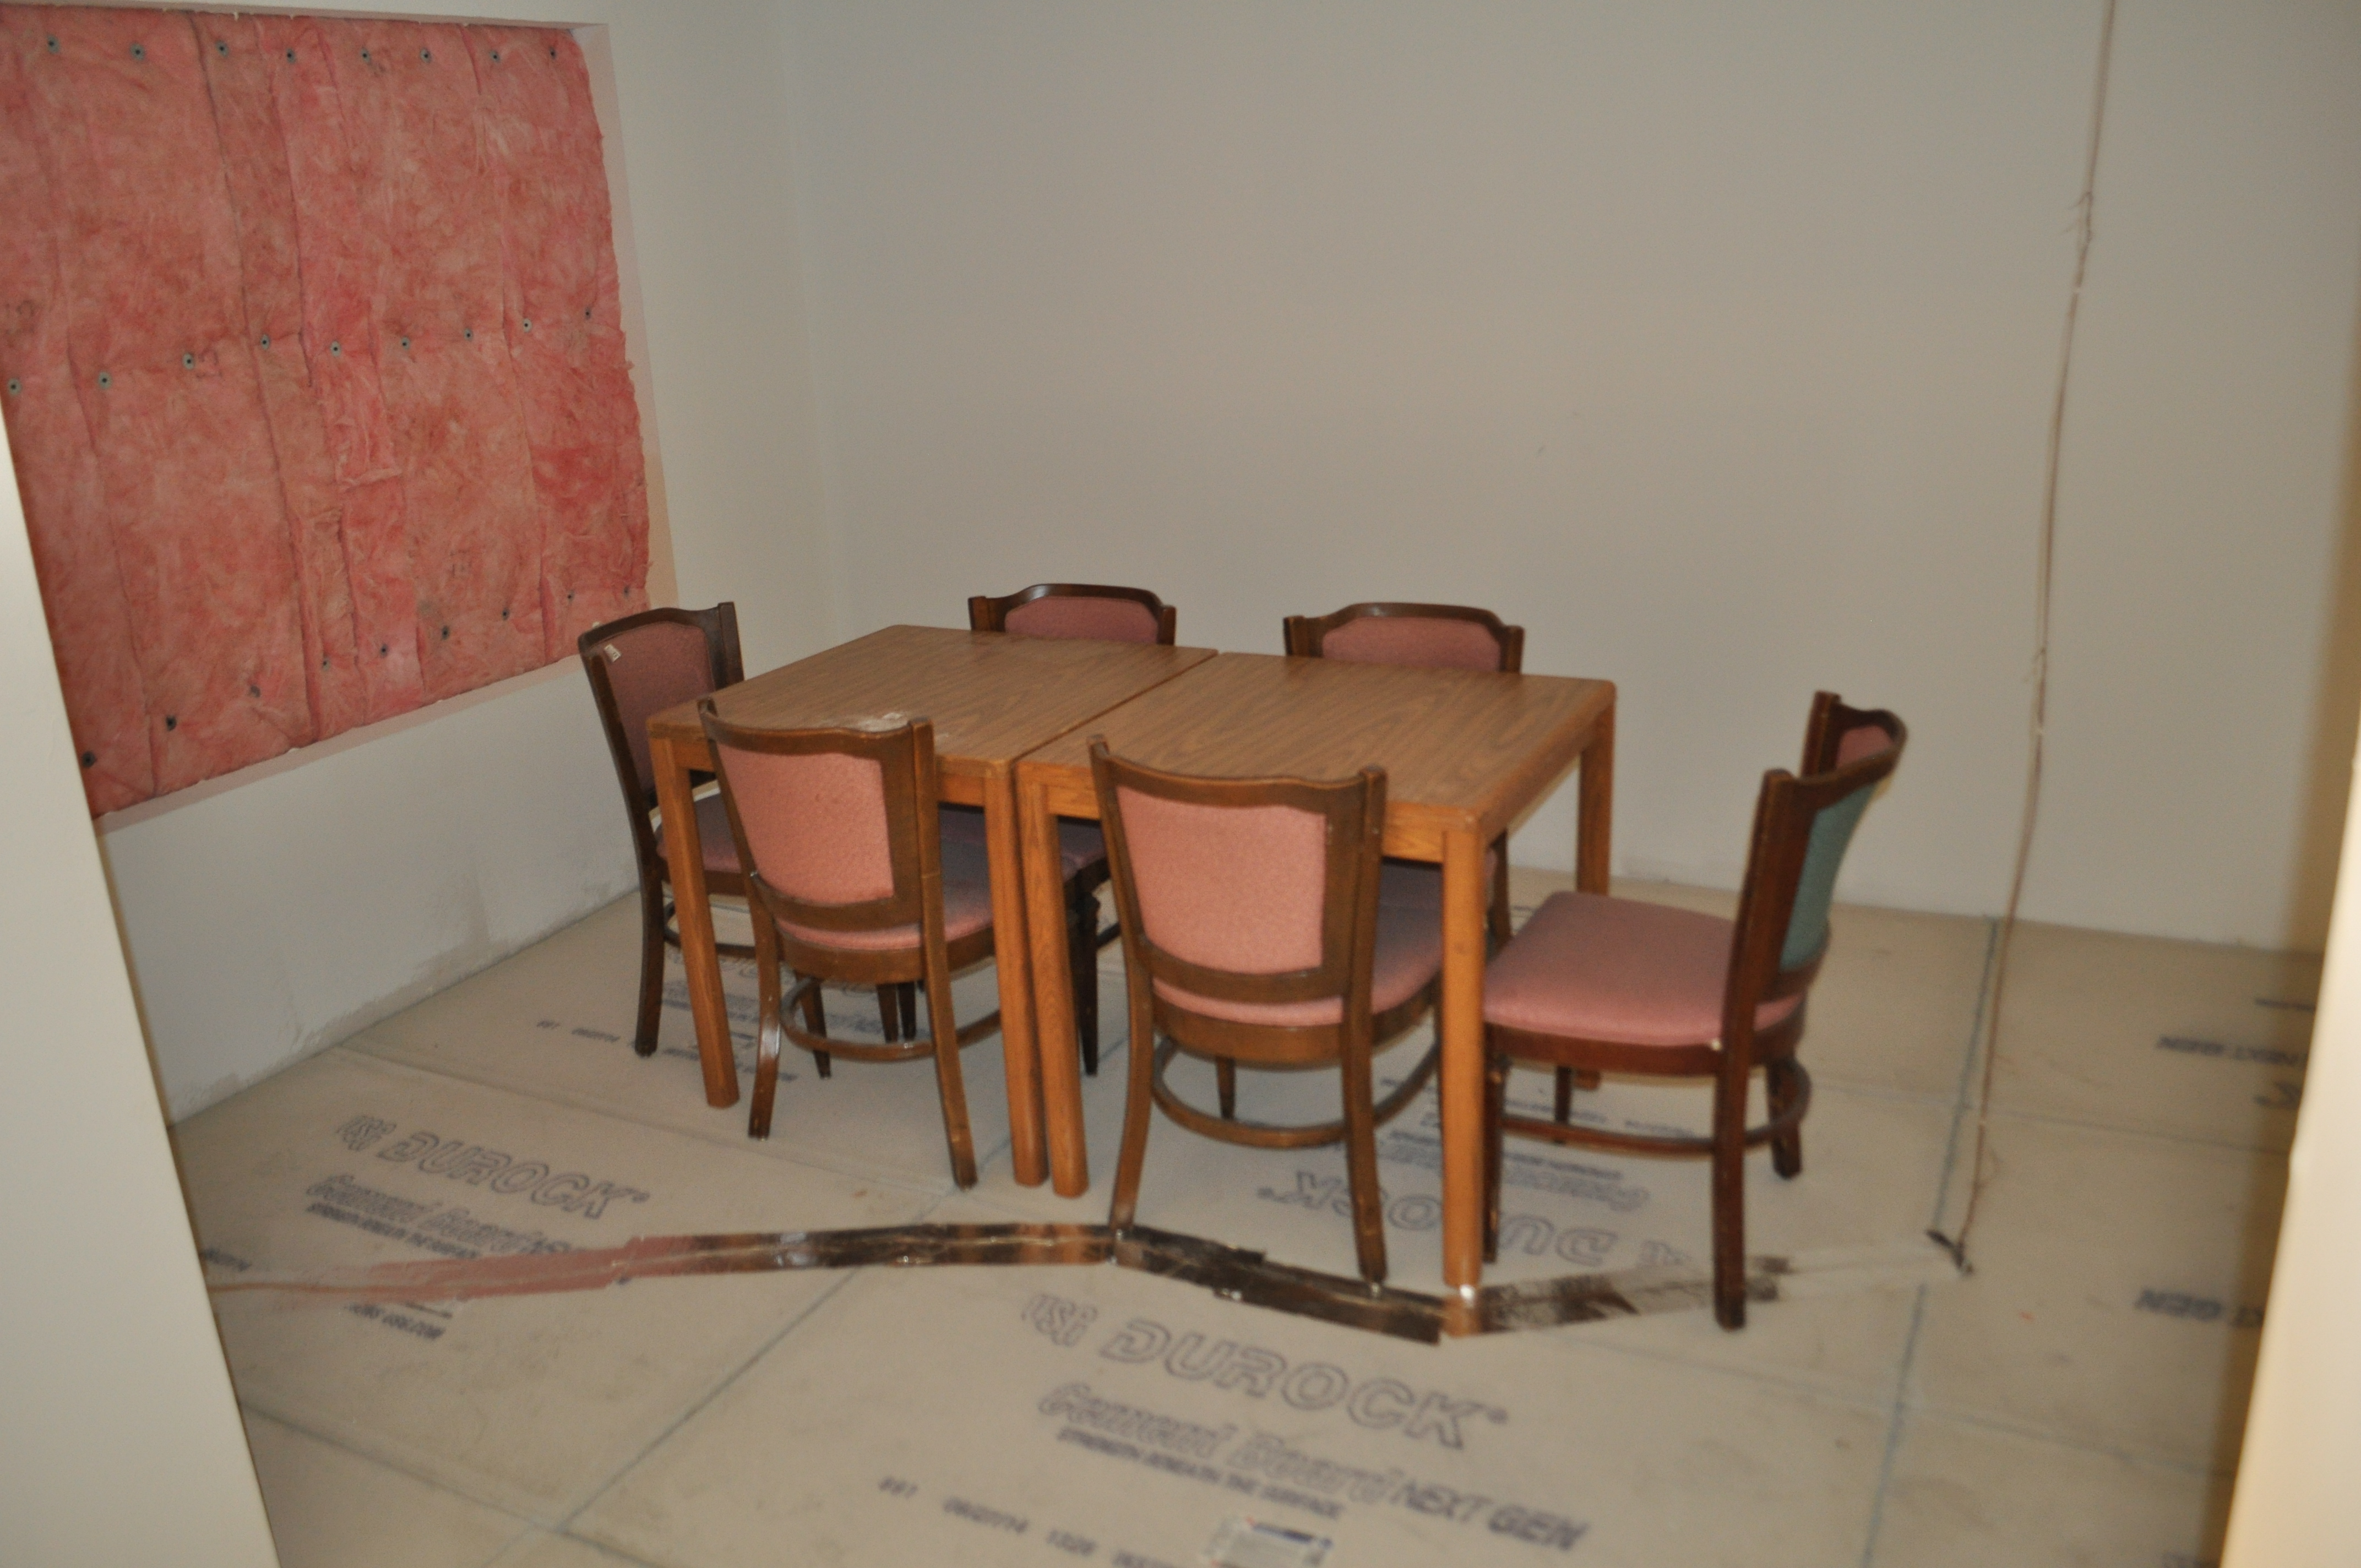
\includegraphics[width=3in]{0_Images/Furniture/2StoryDining.jpg}} \\
	\end{tabular}
	\caption{Dining Room Furniture}
	\label{fig:Dinning}
\end{figure}

The kitchen in the single story was furnished with one table two chairs as the eat in table, as well as a dishwasher, stove, refrigerator and kitchen cabinets with cement board counters. The same appliances, cabinets and counter tops were found in the two story structure with a single table and four chairs. The floors of both rooms were cement board to simulate a tile floor.  Figure \ref{fig:Kitchen} shows the cabinet layout for both the single story and two story kitchens.

\begin{figure}[H]
	\centering
	\begin{tabular}[c]{c c}
		\subfloat[Single Story Kitchen]{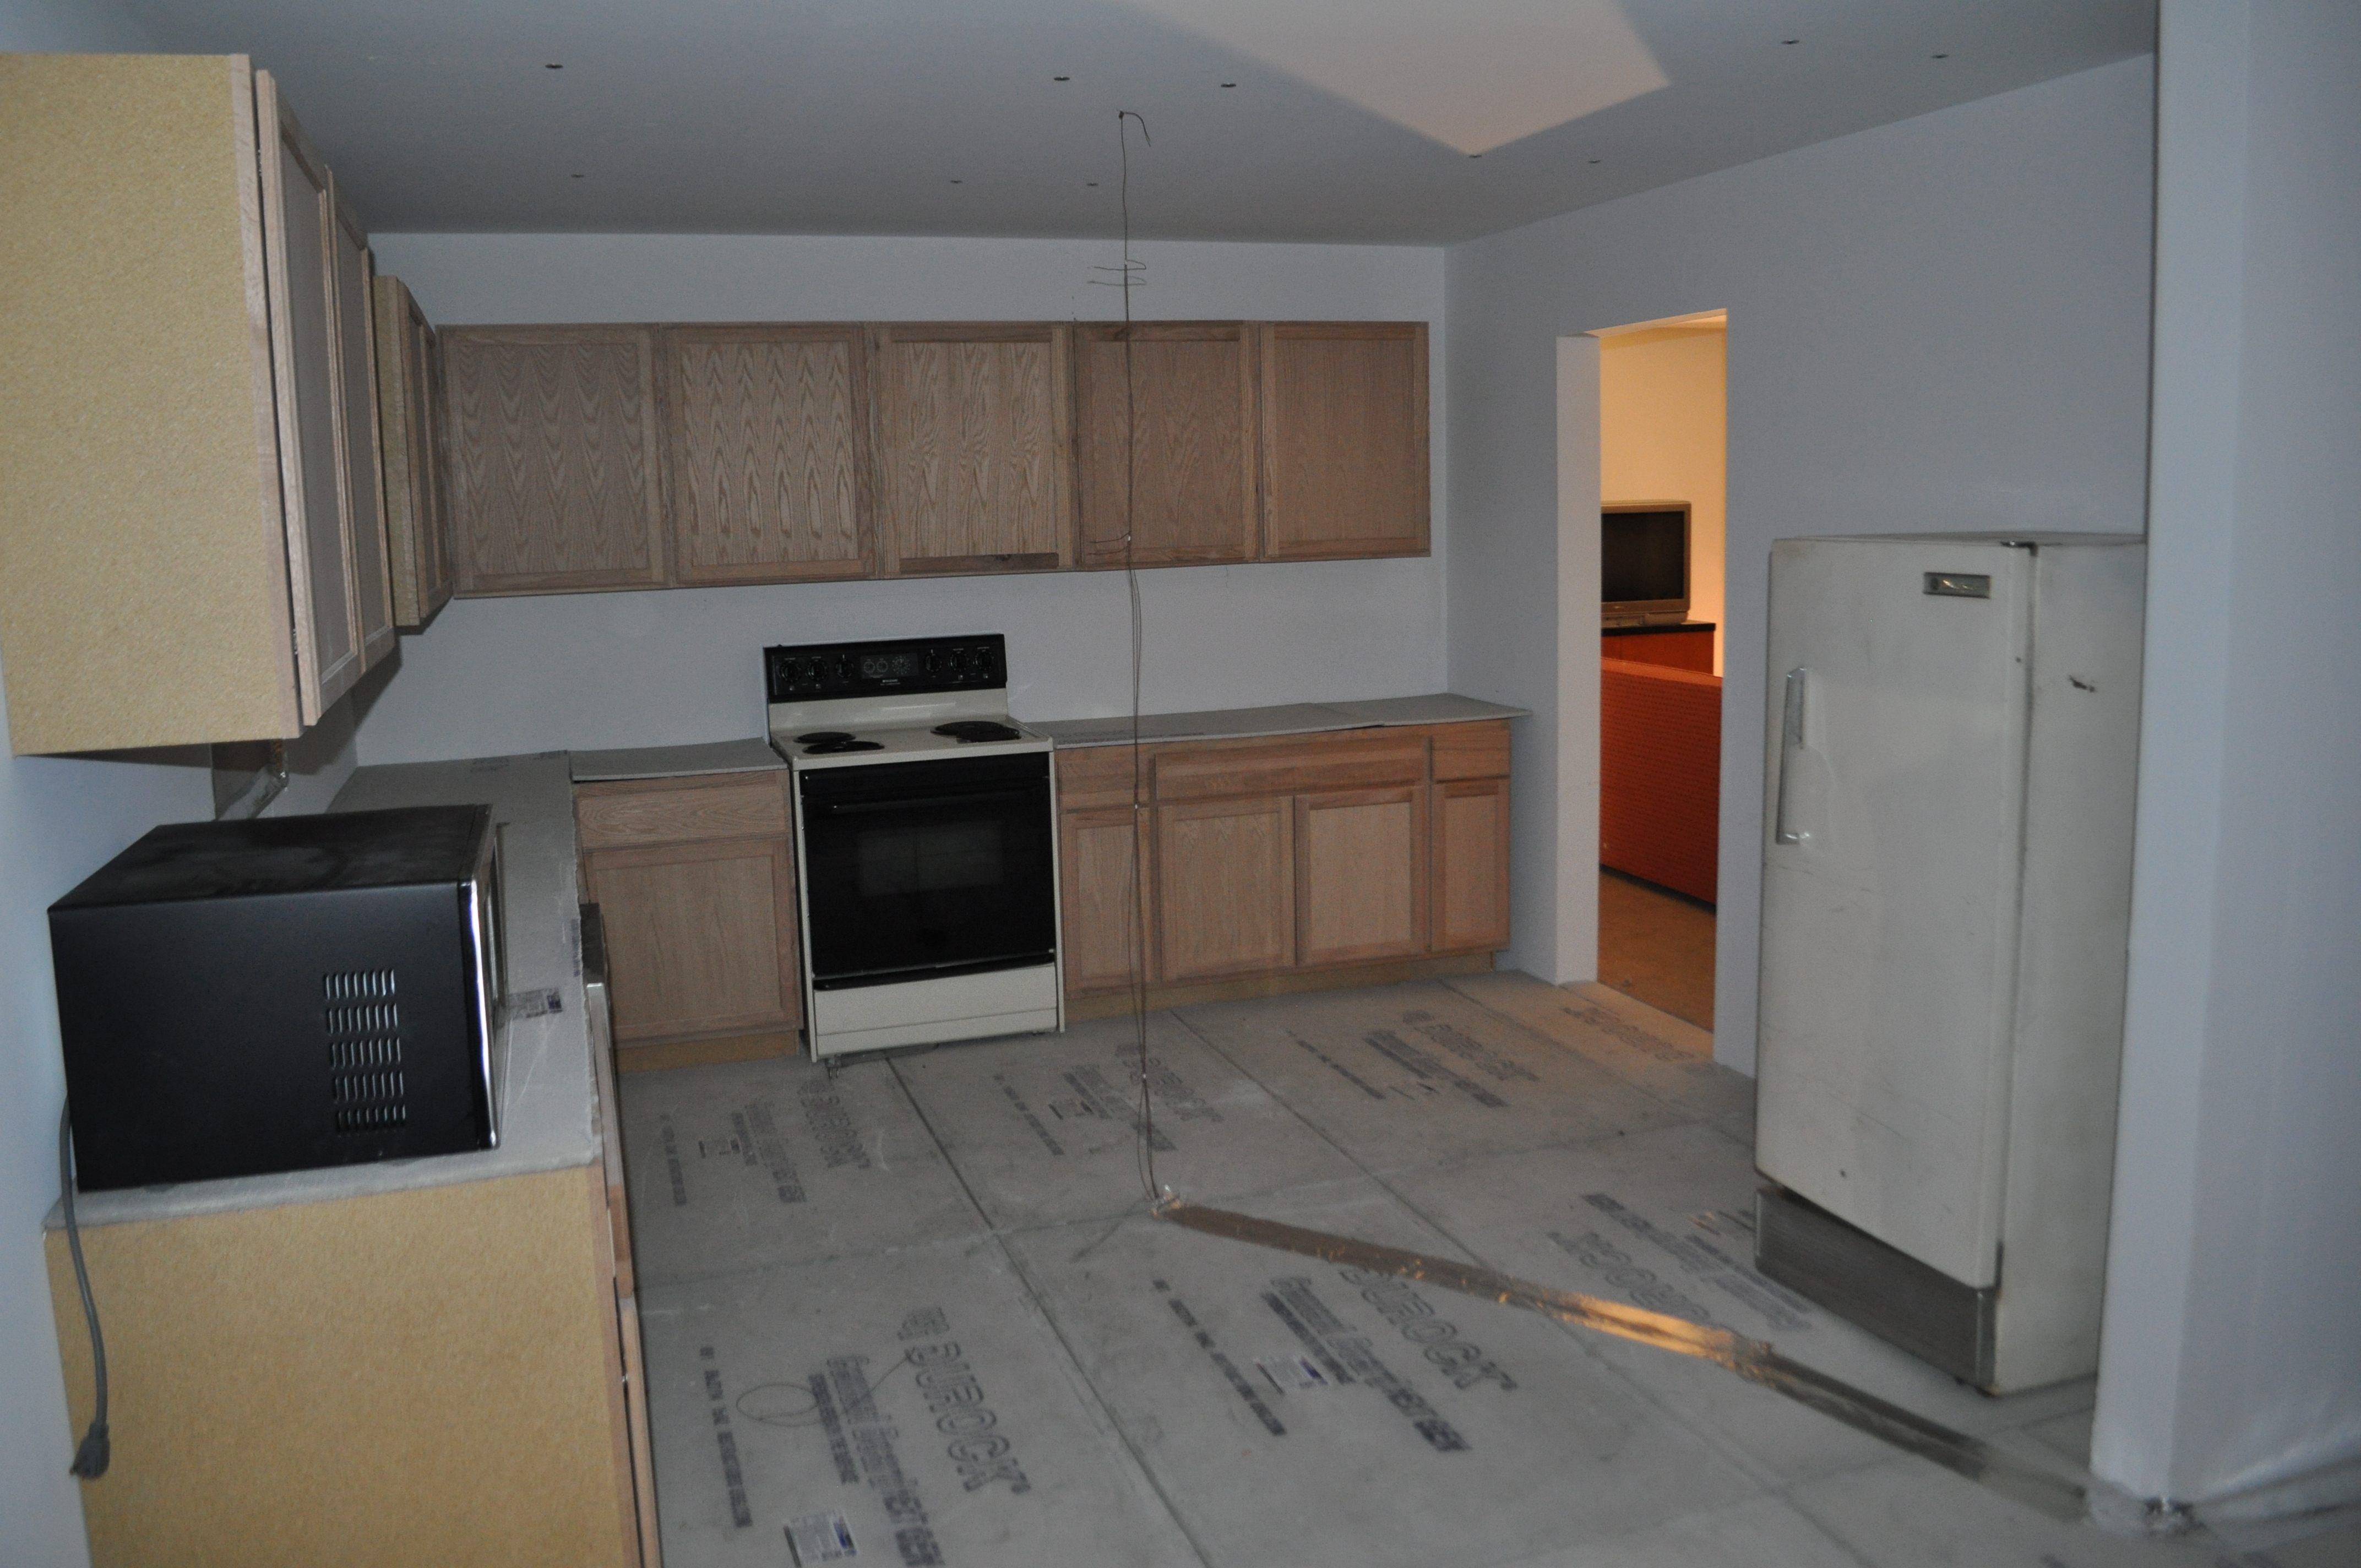
\includegraphics[width=3in]{0_Images/Furniture/1StoryKitchen.jpg}} &
		\subfloat[Two Story Kitchen]{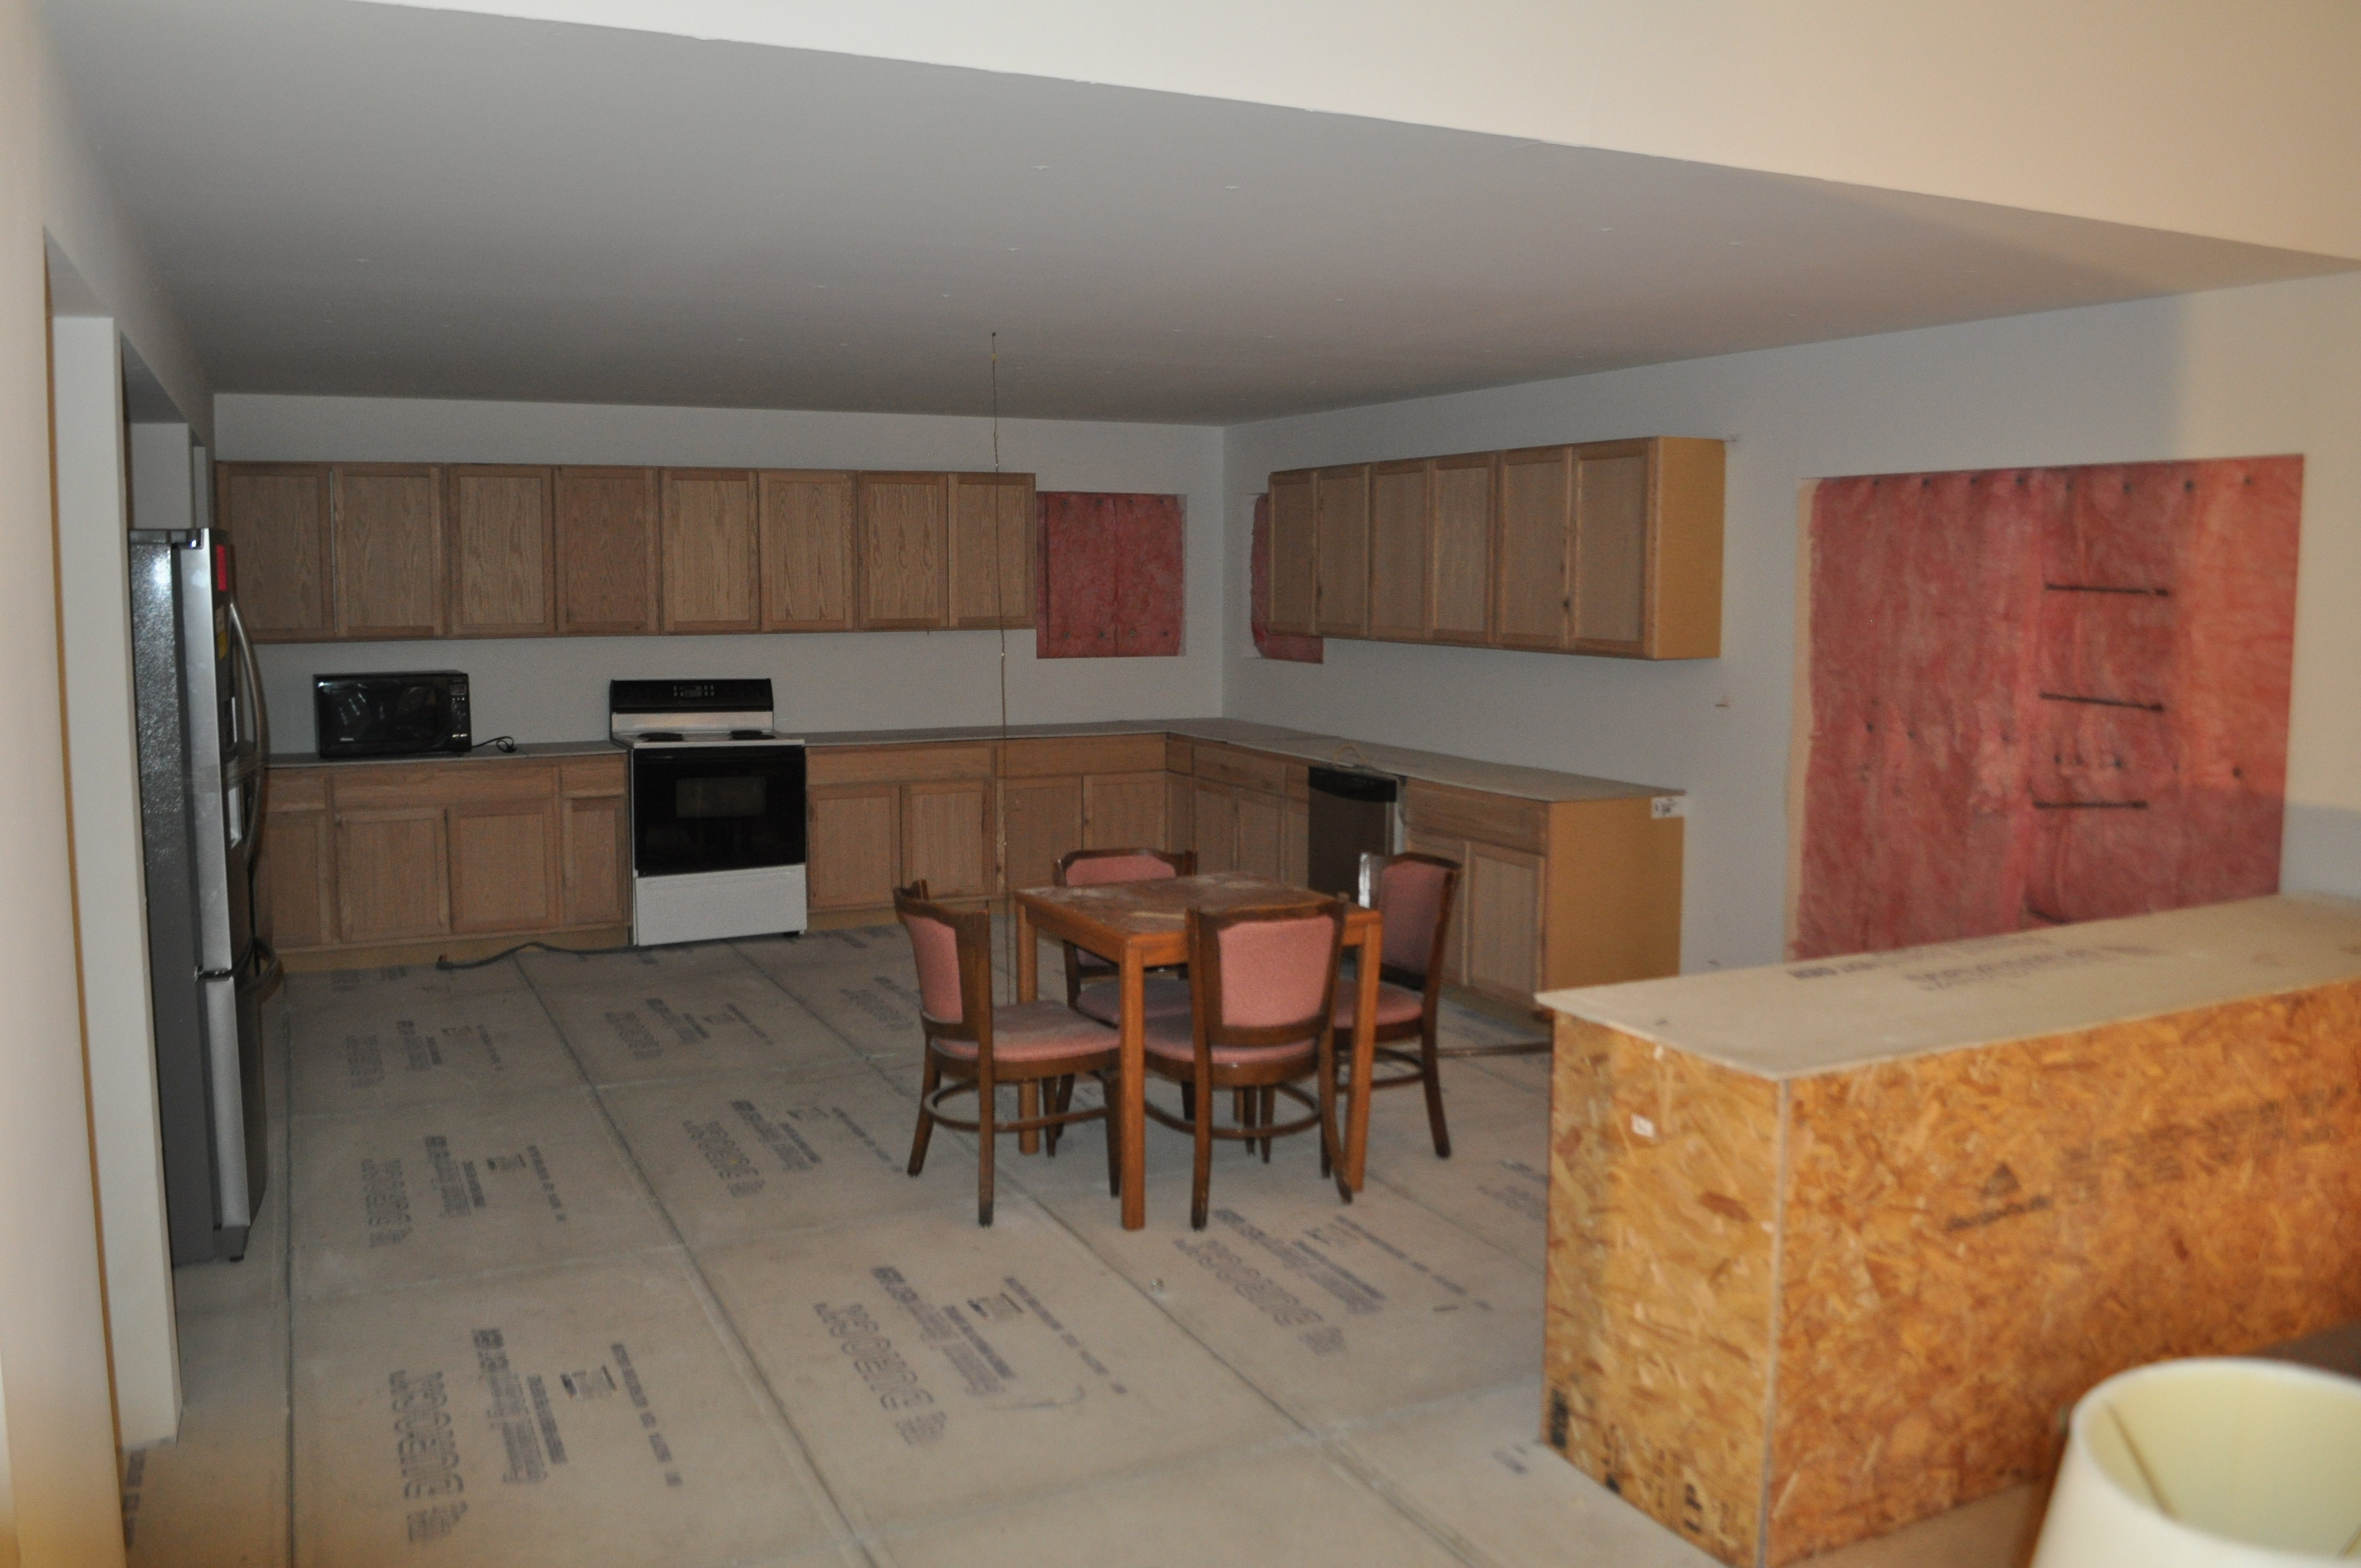
\includegraphics[width=3in]{0_Images/Furniture/2StoryKitchen.jpg}} \\
	\end{tabular}
	\caption{Kitchen Layout}
	\label{fig:Kitchen}
\end{figure}

\begin{figure}[H]
	\centering
	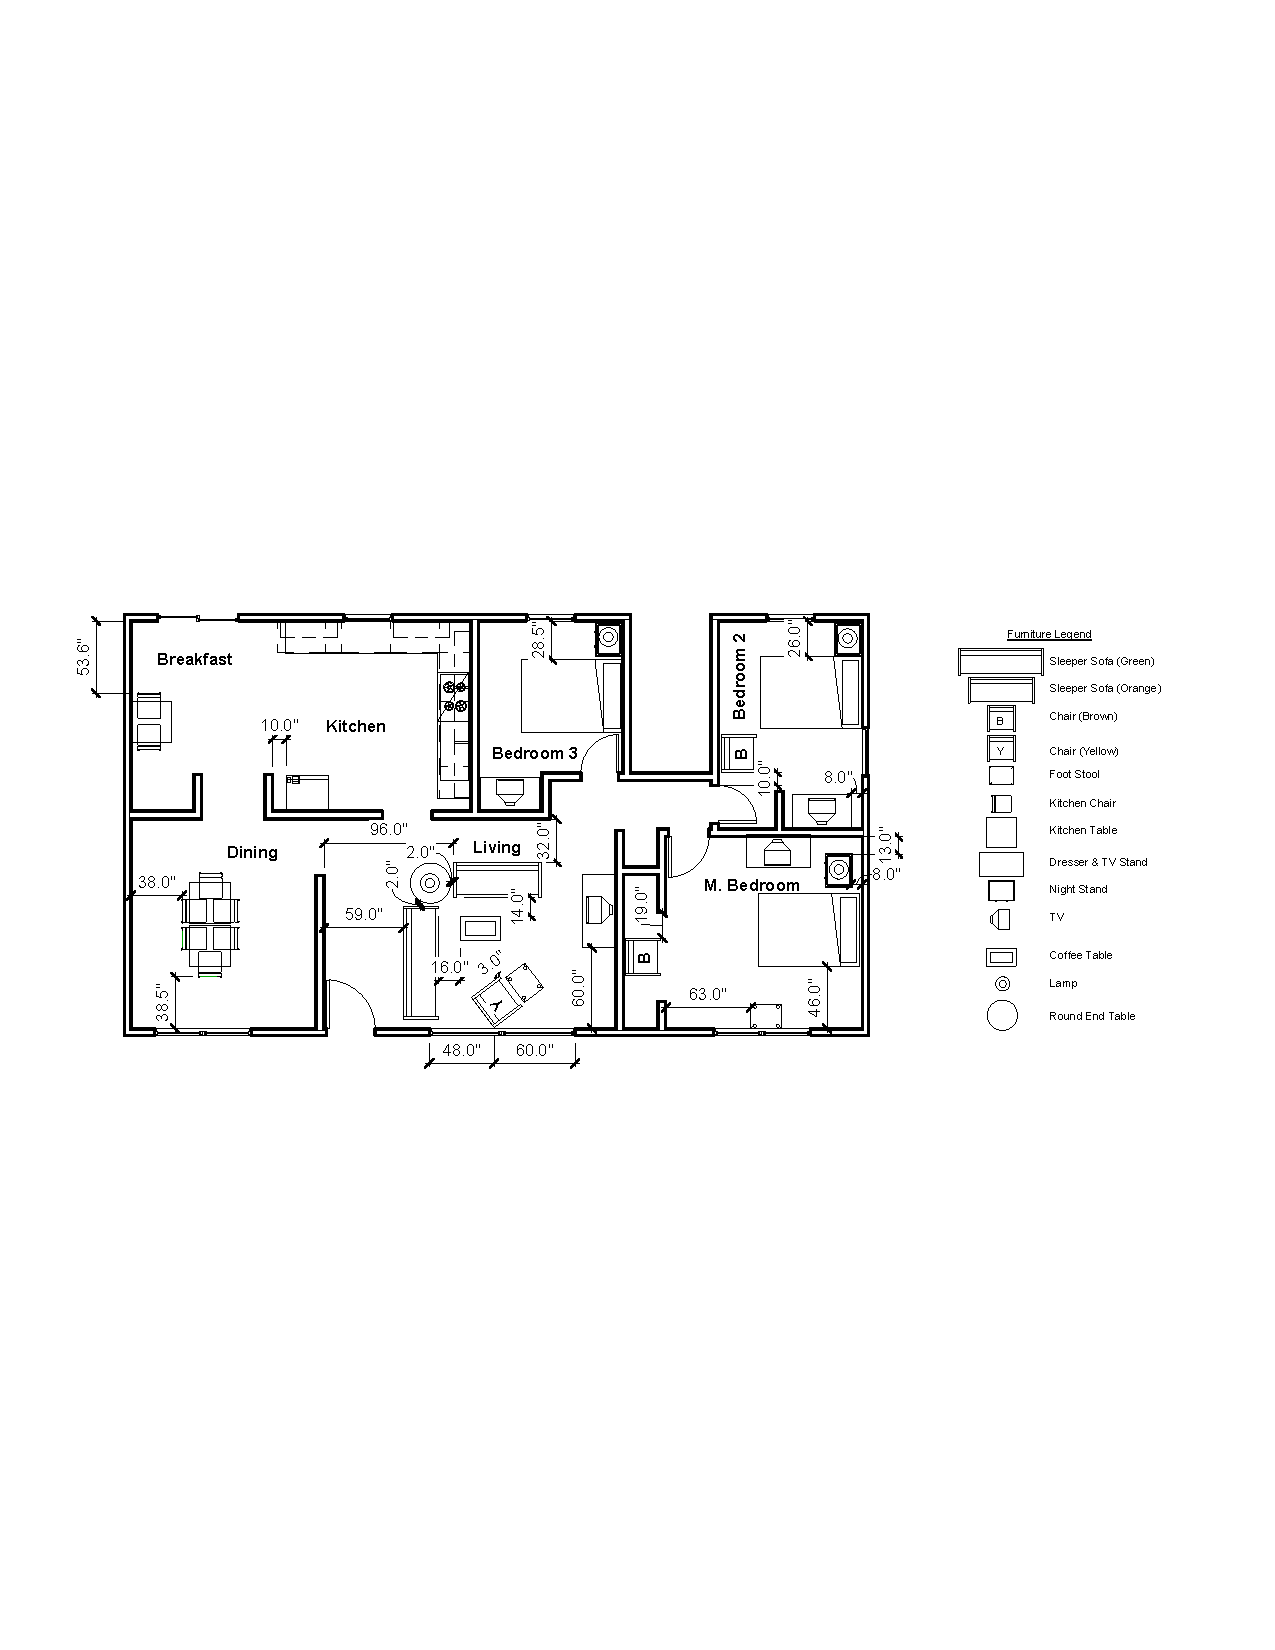
\includegraphics[width=\textwidth]{0_Images/Furniture/Single_Story_Furniture_Layout.pdf}
	\caption{Single Story Furniture Layout}
	\label{fig:SingleStoryFurniture}
\end{figure}

For exact locations and exact quantities of furniture see Figure \ref{fig:SingleStoryFurniture} and Figure \ref{fig:TwoStoryFurniture} for layout and dimensions of furniture. 

\begin{figure}[H]
	\centering
	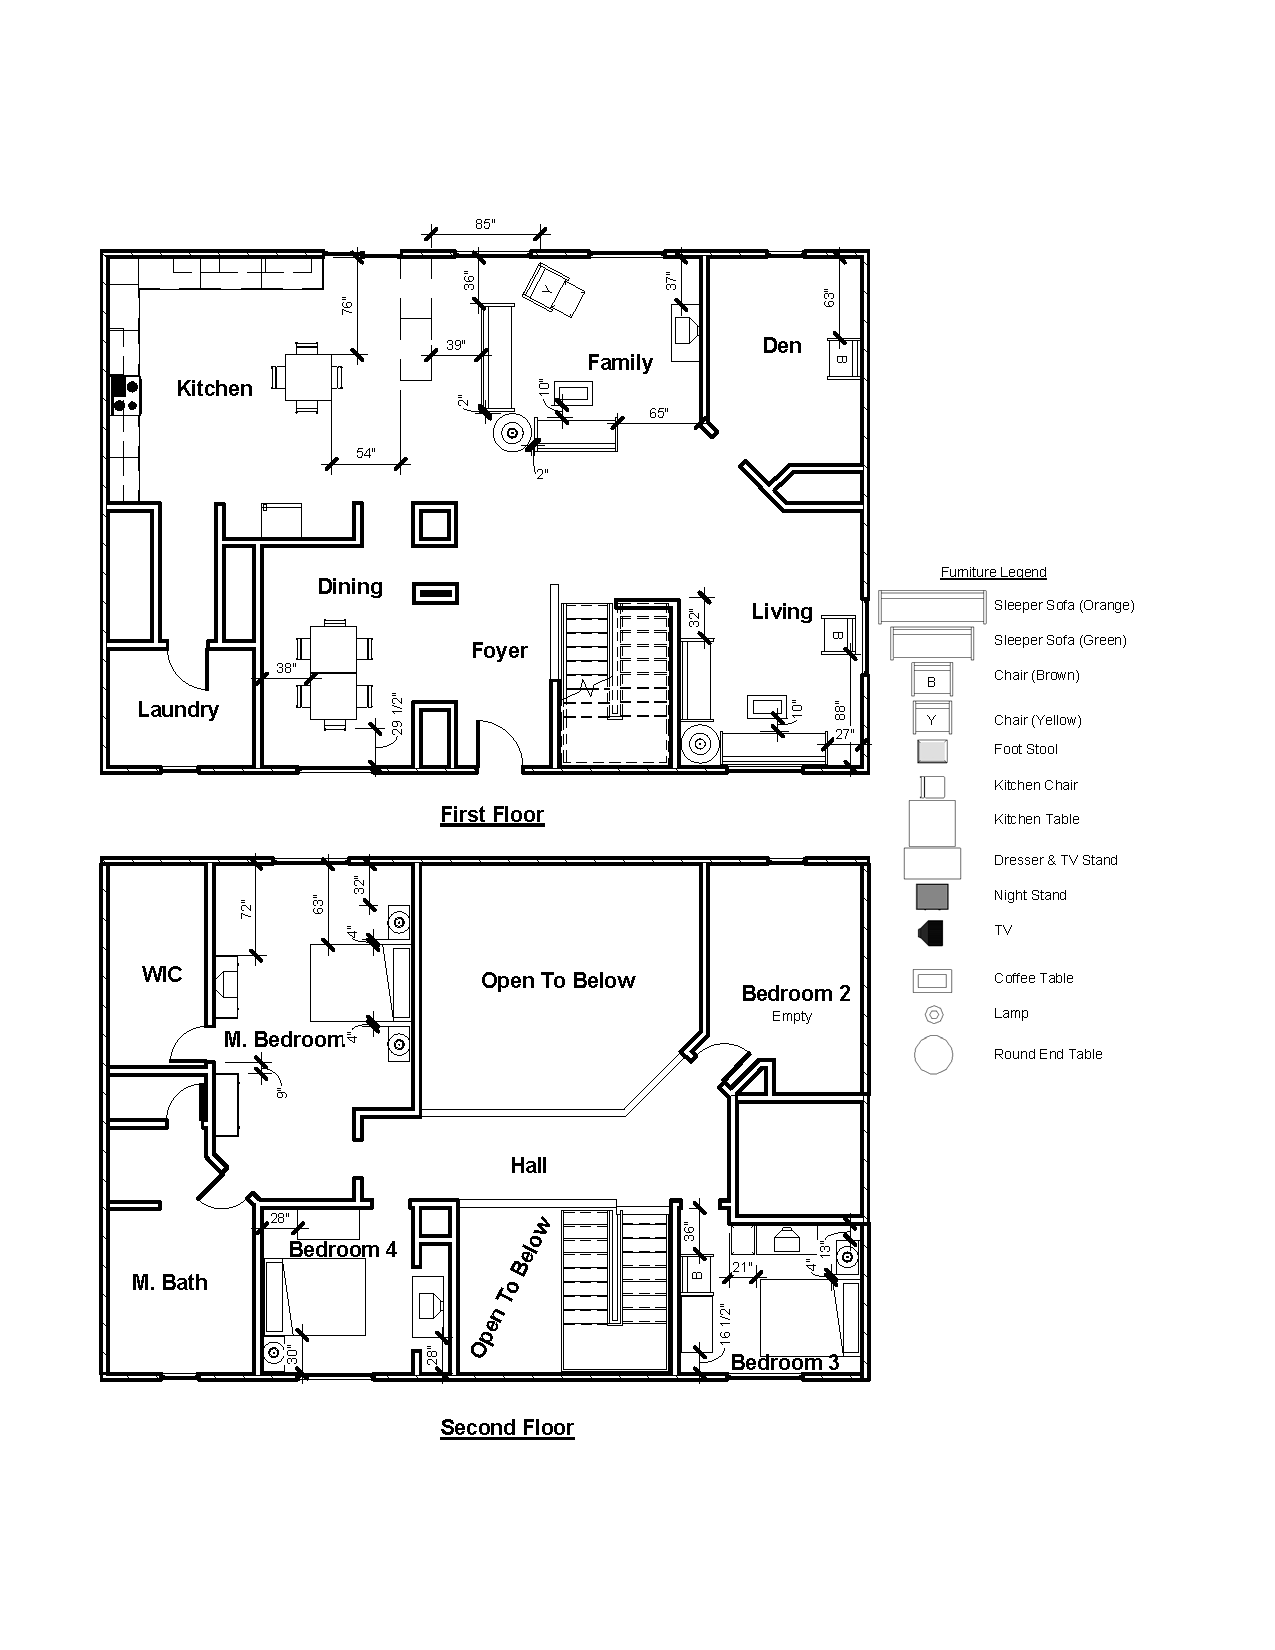
\includegraphics[width=\textwidth]{0_Images/Furniture/Two_Story_Furniture_Layout.pdf}
	\caption{Two Story Furniture Layout}
	\label{fig:TwoStoryFurniture}
\end{figure}

\paragraph{Furniture Heat Release Characterization} \mbox{}

To characterize the foam furniture energy release rates, heat release rate burns were conducted under a cone calorimeter hood. Each piece of furniture was permitted to burn down until a smoldering fire was observed. Table \ref{table:FurnitureHRR_Data} shows the furniture tested and peak heat release rate, total energy released and burnout time for each piece of furniture tested. Figure X shows the furniture tested. 

\begin{table}[H]
	\caption{Furniture Heat Release Data}
	\begin{tabular}{|c|c|c|c|}
		\hline
		Furniture & Peak Heat Release Rate (kW) & Total Energy Released (MJ) & Burn duration \\ \hline \hline
		Chair (Yellow) 1 & 845 & 145 & 14:45 \\ \hline
		Chair (Yellow) 2 & 1094 & 123 & 15:00 \\ \hline
		Chair (Yellow) 3 & 1236 & 128 & 15:00 \\ \hline
		Chair (Brown) 1 & 1841 & 458 & 19:45 \\ \hline
		Chair (Brown) 2 & 1473 & 451 & 19:45 \\ \hline
		Chair (Brown) 3 & 1410 & 391 & 19:45 \\ \hline
		Sleeper Sofa (Orange) 1  & 2441 & 632 & 22:46 \\ \hline
		Sleeper Sofa (Orange) 2  & 1897 & 663 & 22:44 \\ \hline
		Sleeper Sofa (Orange) 3  & 2083 & 613 & 23:10 \\ \hline
		Sleeper Sofa (Green) 1  & 3543 & 968 & 24:44 \\ \hline
		Sleeper Sofa (Green) 2  & 2894 & 1071 & 24:44 \\ \hline
		Sleeper Sofa (Green) 3  & 2640 & 1071 & 24:45 \\ \hline
		Bed 1 & 1306 & 873 & 50:00 \\ \hline
		Bed 2 & 1399 & 709 & 53:23 \\ \hline
	\end{tabular}
	\label{table:FurnitureHRR_Data}
\end{table}

The results of the Chair (Yellow) heat release rate characterization burns is shown in Figure \ref{fig:YellowChairHRR}. The growth of the Chair (Yellow) was very similar with all three chairs tested with peak heat release rates occurring within 5 minutes to 5 minutes and 30 seconds of ignition. The Yellow Chair 3 grew slightly slower however provided the highest total energy released. Results for peak heat release rate were within 391kW between minimum and maximum, the total energy released was within 22MJ of between the minimum and maximum. 

\begin{figure}[H]
	\centering
	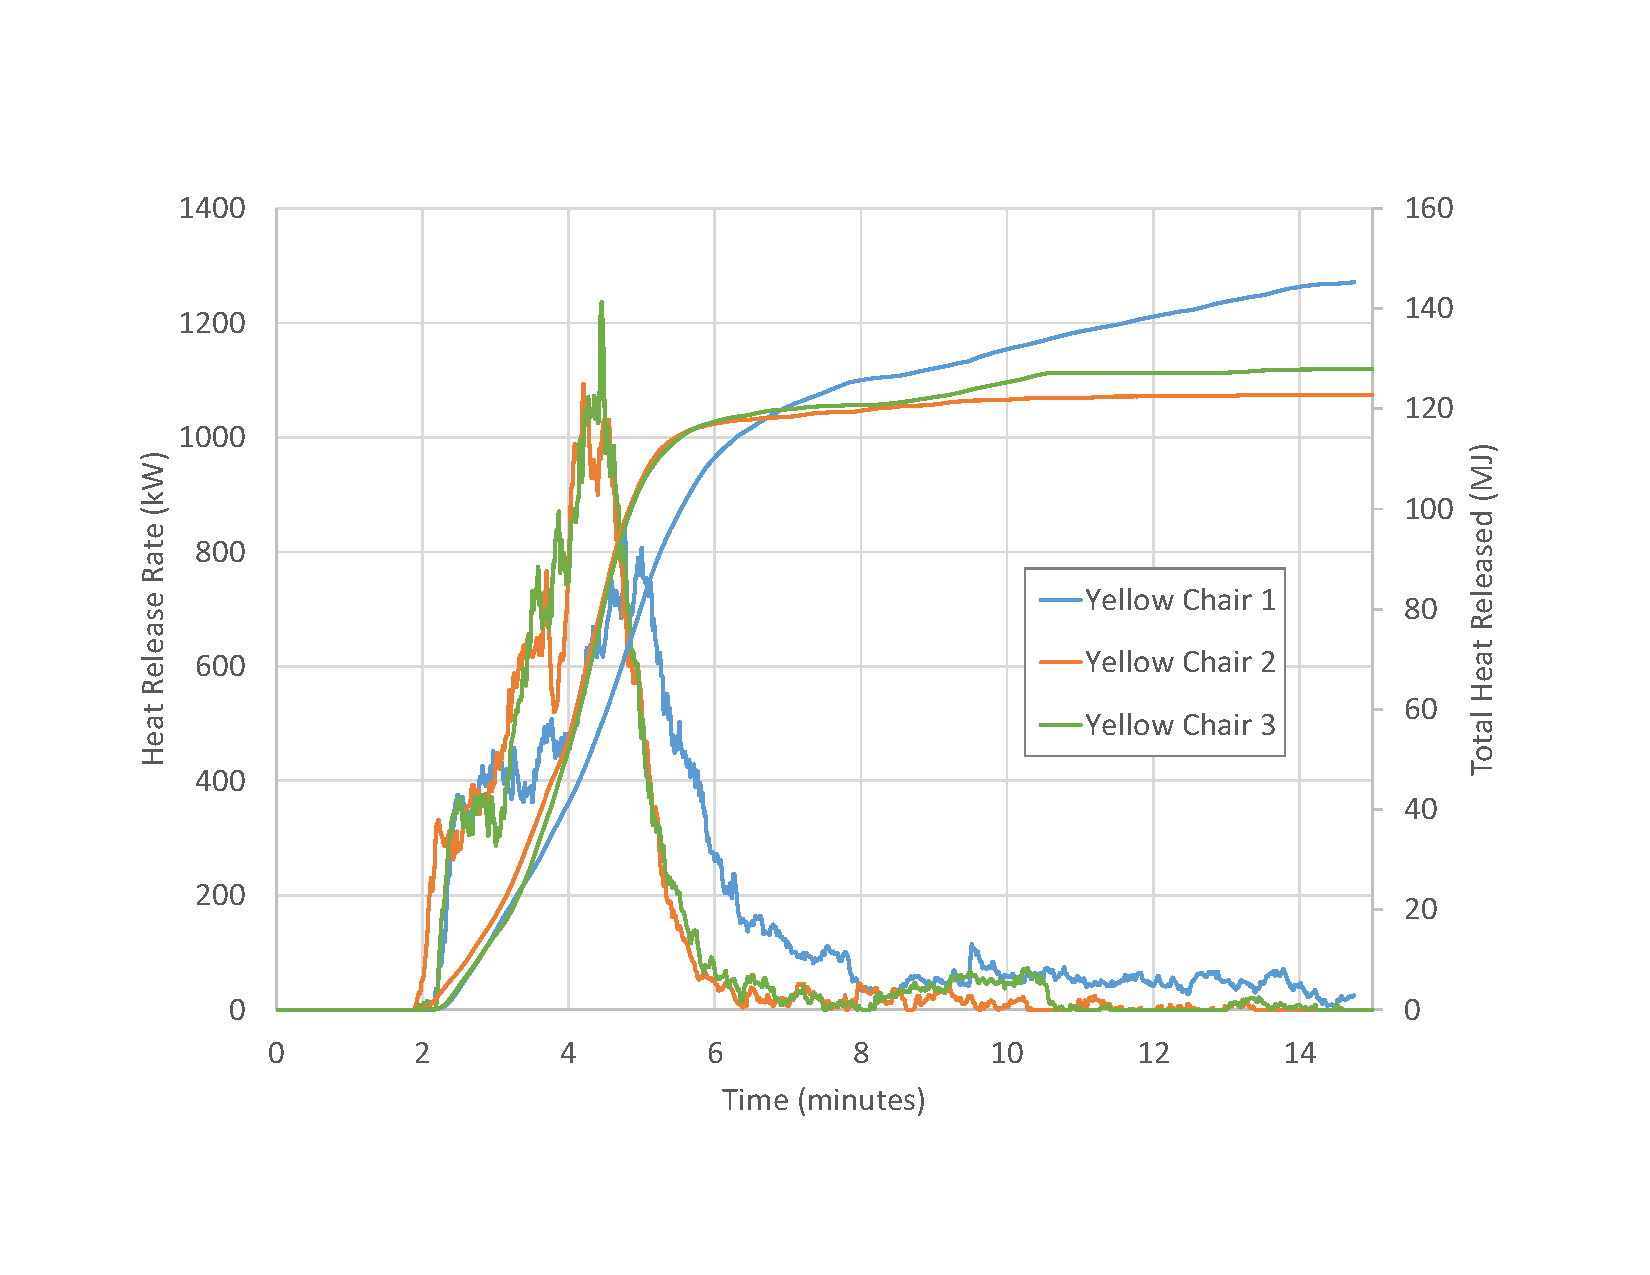
\includegraphics[width=\textwidth]{0_Images/Furniture/ChairYellow_HRR.pdf}
	\caption{Chair (Yellow) Heat Release Rate Characterization Results}
	\label{fig:YellowChairHRR}
\end{figure}

The results of the Chair (Brown) heat release rate characterization burns is shown in Figure \ref{fig:BrownChairHRR}. The growth of the Chair (Brown) was very similar with all three chairs tested with peak heat release rates occurring within 4 and 45 Seconds to 5 minutes of ignition. The Brown Chair 1 grew slightly faster however provided the same total energy released as the Brown Chair 2. The Brown Chair 3 grew the slowest and provided the smallest total energy release. Results for peak heat release rate were within 431kW between minimum and maximum, the total energy released was within 67MJ of between the minimum and maximum. 

\begin{figure}[H]
	\centering
	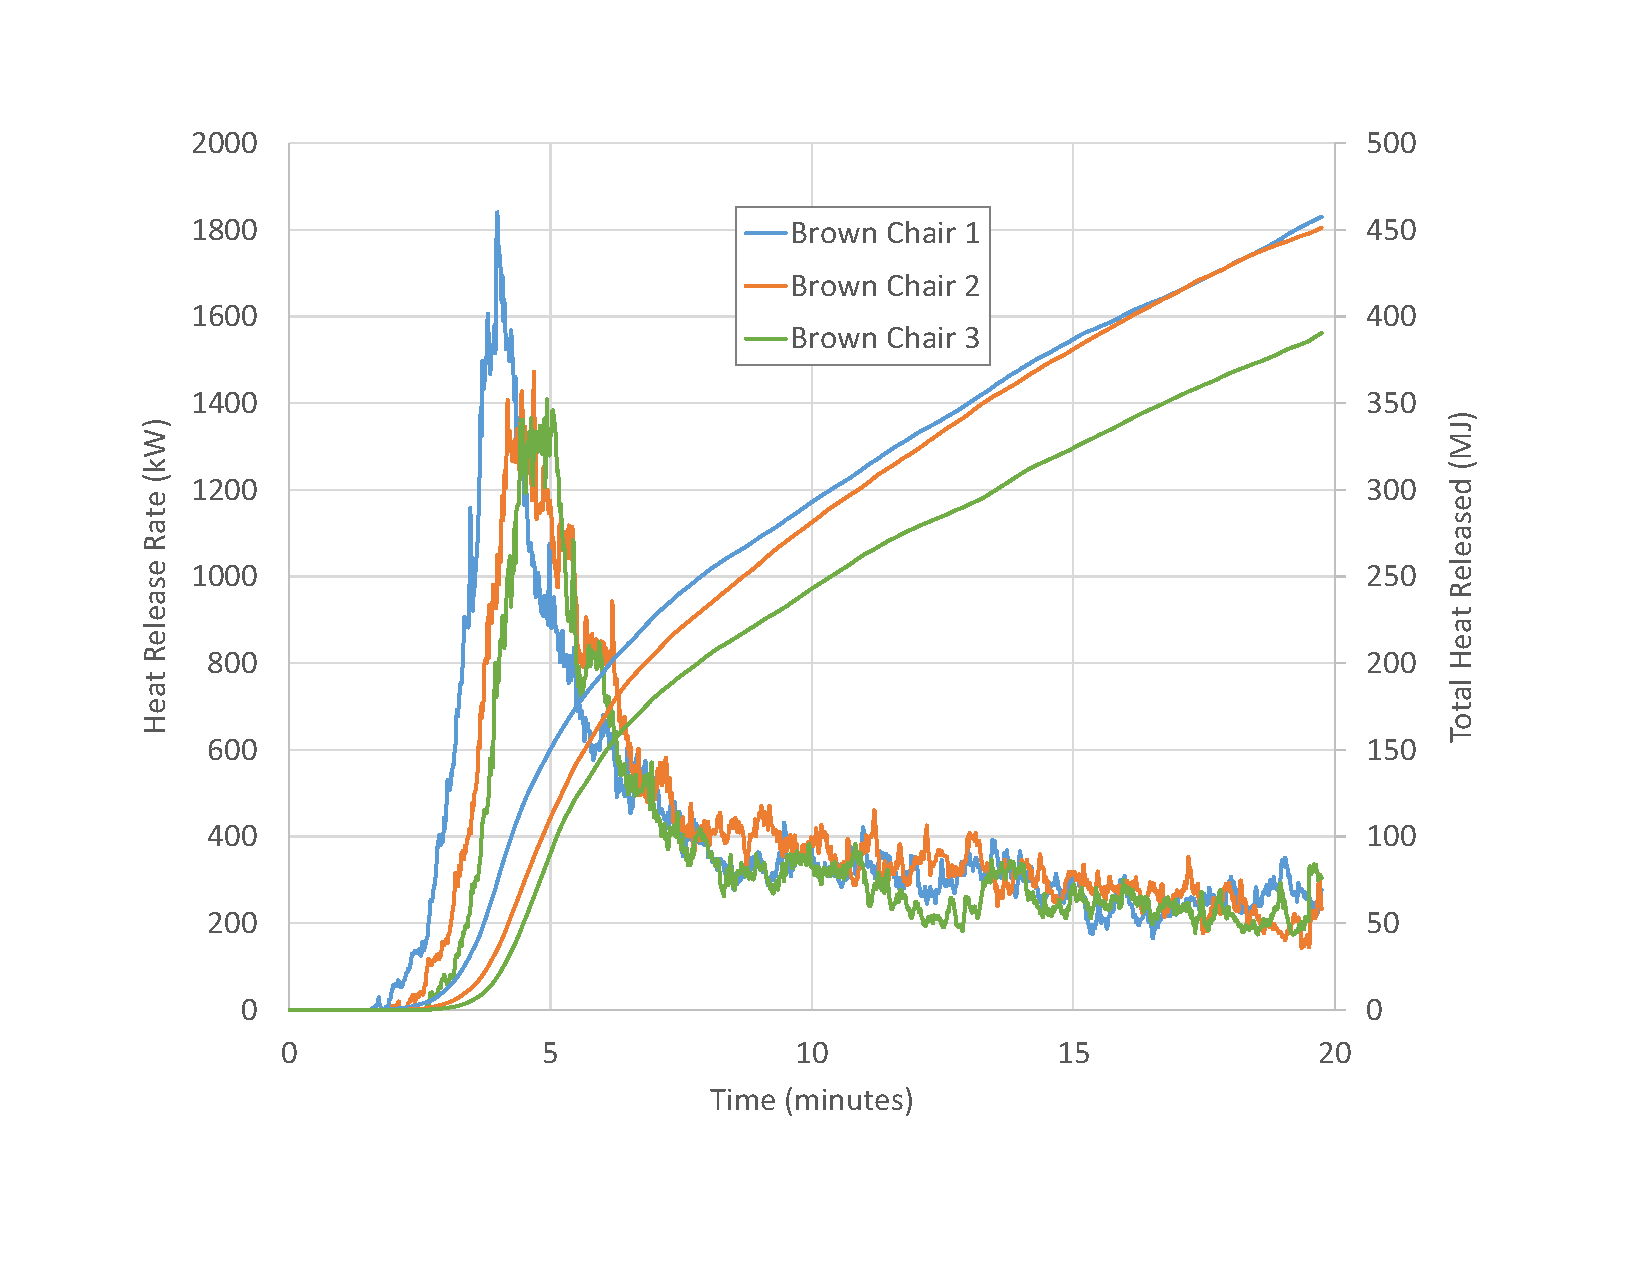
\includegraphics[height=0.45\textheight]{0_Images/Furniture/BrownChair_HRR.pdf}
	\caption{Chair (Brown) Heat Release Rate Characterization Results}
	\label{fig:BrownChairHRR}
\end{figure}

The results of the Sleeper Sofa (Orange) heat release rate characterization burns is shown in Figure \ref{fig:SofaOrangeHRR}. The growth of the Sleeper Sofa (Orange) was very similar with all three chairs tested with peak heat release rates occurring within 5 and 50 Seconds to 5 minutes and 10 seconds of ignition. Results for peak heat release rate were within 544kW between minimum and maximum, the total energy released was within 50MJ of between the minimum and maximum. 

\begin{figure}[H]
	\centering
	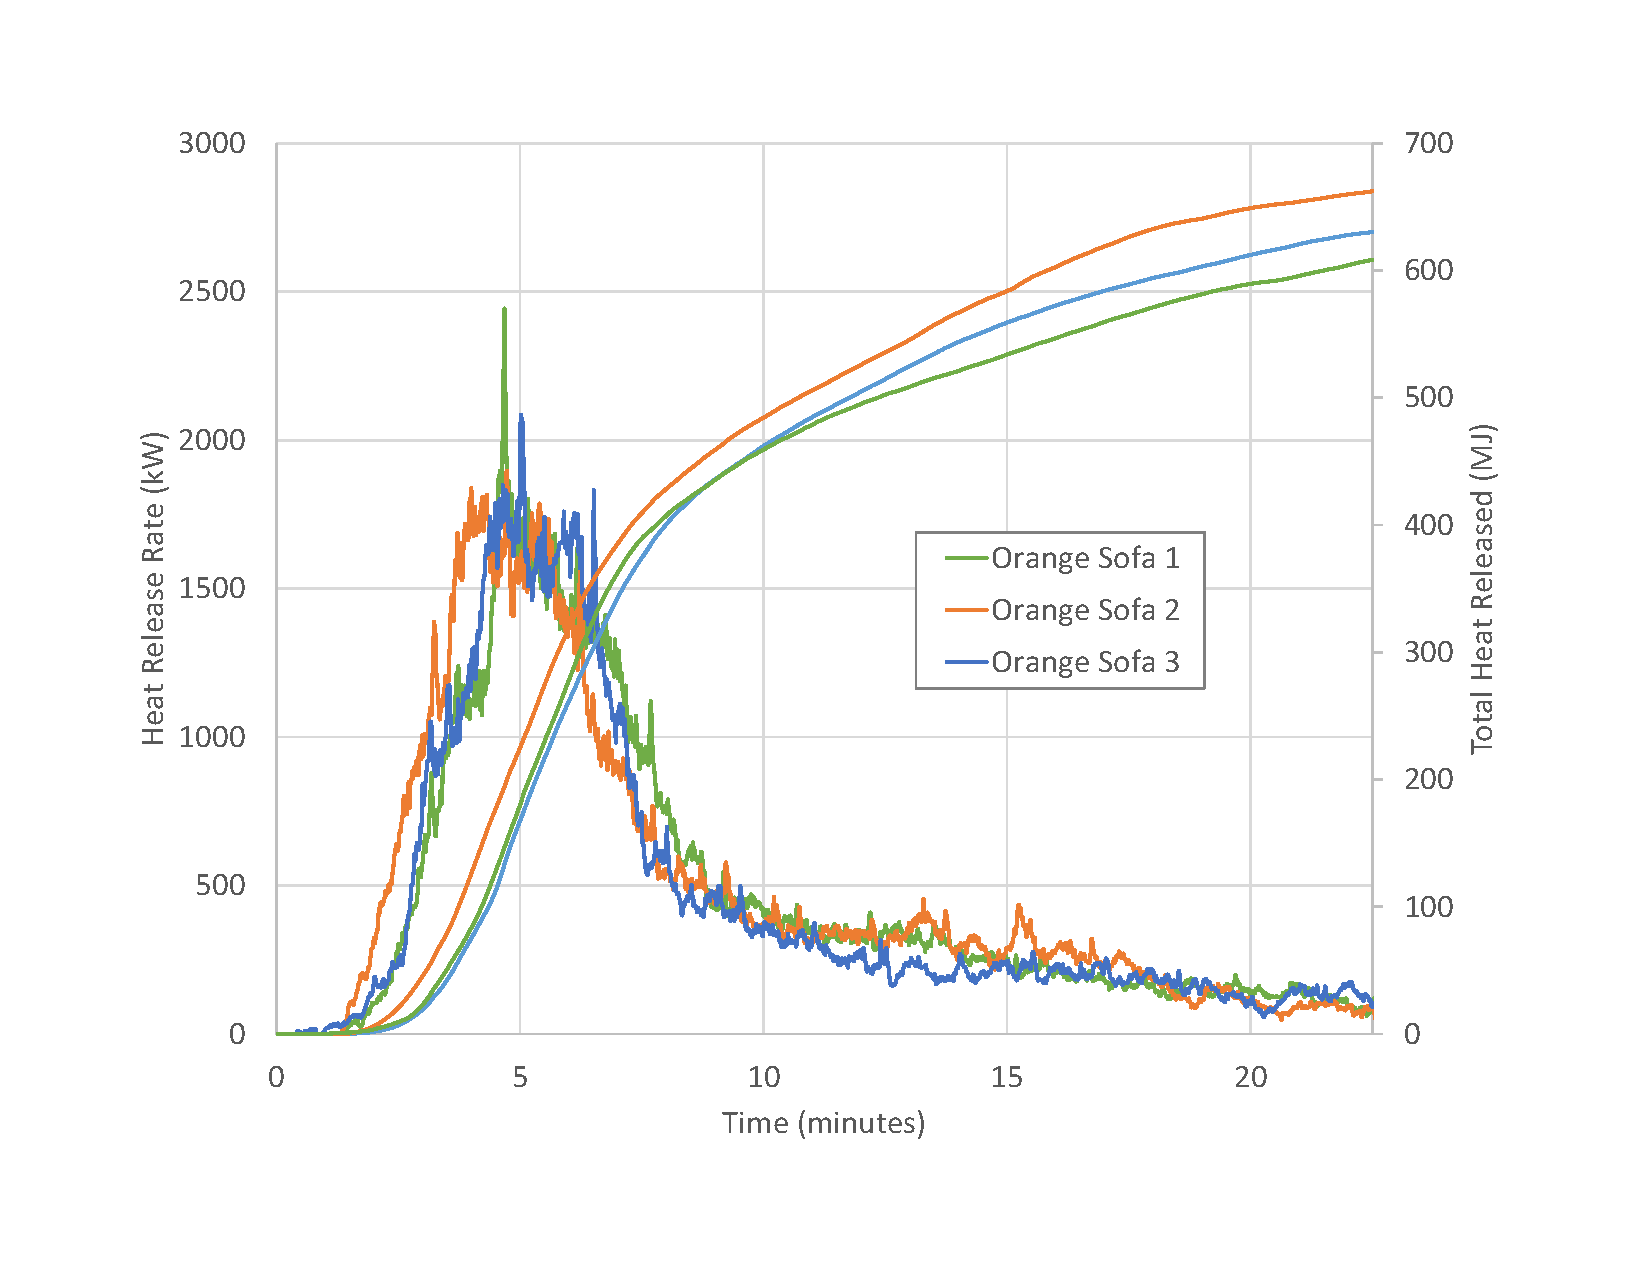
\includegraphics[height=0.45\textheight]{0_Images/Furniture/Sofa_Orange_HRR.pdf}
	\caption{Sleeper Sofa (Orange) Heat Release Rate Characterization Results}
	\label{fig:SofaOrangeHRR}
\end{figure}

The results of the Sleeper Sofa (Green) heat release rate characterization burns is shown in Figure \ref{fig:SofaOrangeHRR}. The growth of the Sleeper Sofa was very similar with all three chairs tested with peak heat release rates occurring within 6 to 7 minutes of ignition. Results for peak heat release rate were within 903kW between minimum and maximum, the total energy released was within 103MJ of between the minimum and maximum. 

\begin{figure}[H]
	\centering
	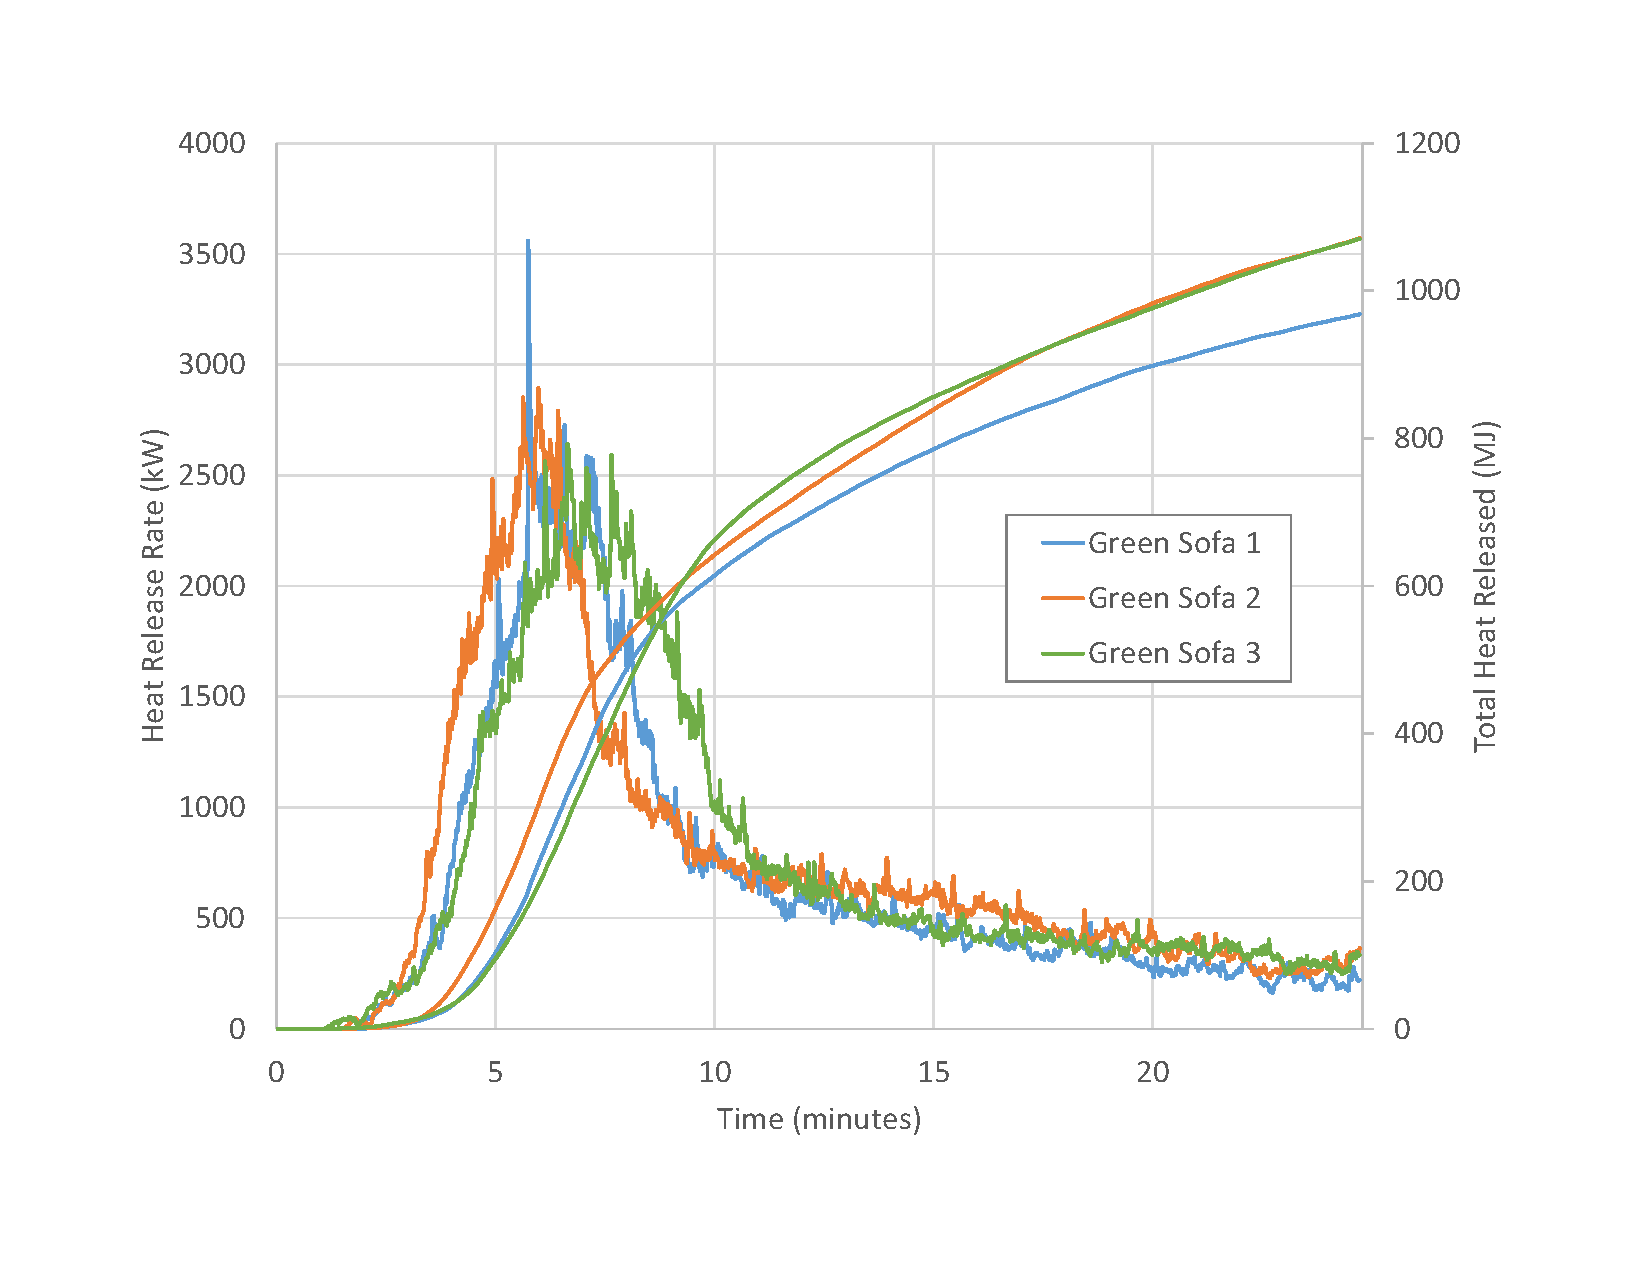
\includegraphics[height=0.45\textheight]{0_Images/Furniture/Sofa_Green_HRR.pdf}
	\caption{Sleeper Sofa (Green) Heat Release Rate Characterization Results}
	\label{fig:SofaGreenHRR}
\end{figure}

The results of the bed heat release rate characterization burns is shown in Figure \ref{fig:BedHRR}. The growth of the Beds was significantly different as the fire had to burn across the top of the comforter and down before involving the matress and reaching its peak heat release rate at approximately 38 minutes for bed 1 and 45 minutes for bed 2. Although the growth rate differed the results of the peak heat release rate were within 93kW between minimum and maximum, the total energy released was within 164MJ of between the minimum and maximum. The difference in the total energy release can be explained due to the different growth rates and time frame associated with each.

\begin{figure}[H]
	\centering
	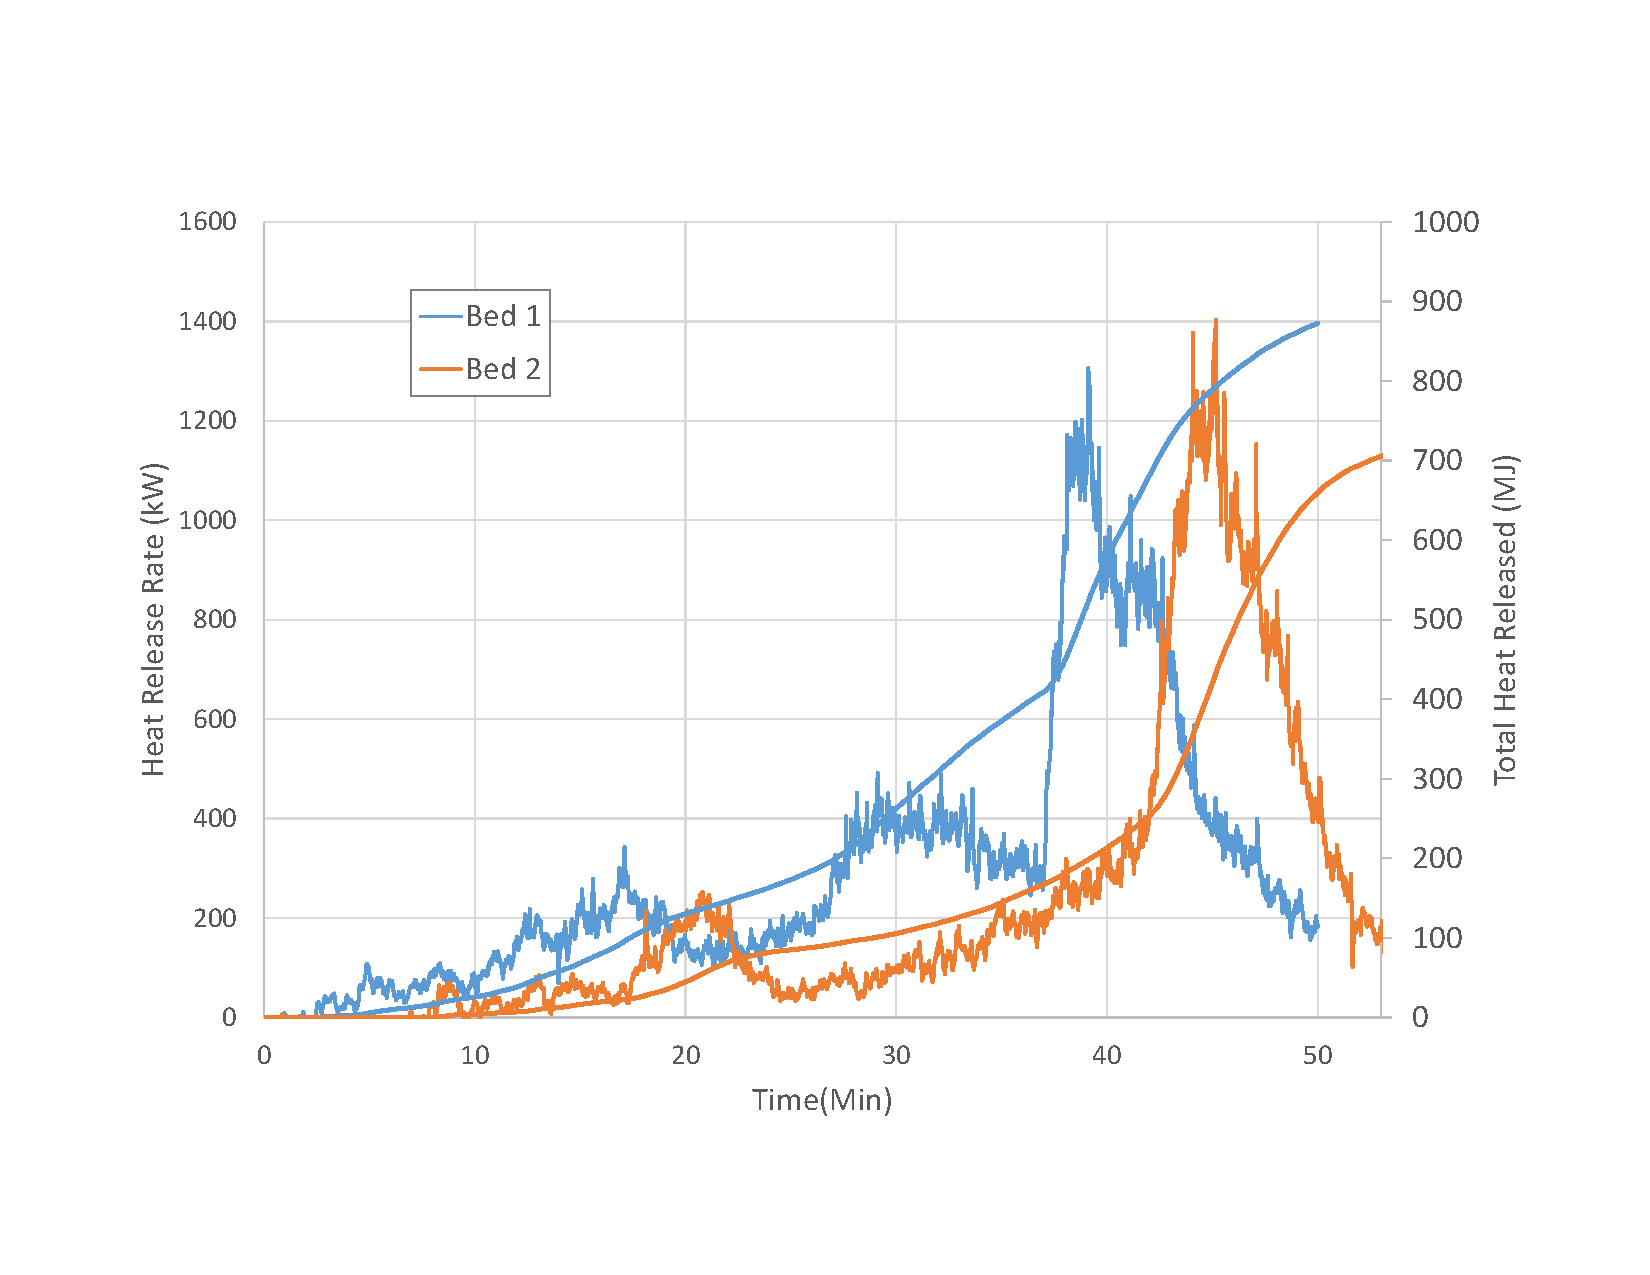
\includegraphics[height=0.45\textheight]{0_Images/Furniture/Bed_HRR.pdf}
	\caption{Bed Heat Release Rate Characterization Results}
	\label{fig:BedHRR}
\end{figure}

\subsection{Ventilation Limited Room Burns}
A fire burns in direct proportion to the available oxygen. Past studies conducted under the Department of Homeland Securities Assistance to firefighters grants have established a basis of this for both single compartment fires along with fires within a residential structure \cite{DHS2008} \cite{DHS2010}. In order to provide further understanding of this concept two room scale experiments were conducted under a cone calorimeter hood to evaluate the energy release rate as it compares to the fuel load in a single compartment fire, on furnished and one over furnished.

Each compartment measured 12ft long by 12ft wide and 8ft tall, with a front opening of 7ft - 10$\frac{3}{4}$in wide by 8ft high. The walls were wood stud frame 16in on center with $\frac{1}{2}$in type X gypsum wall board. The ceiling was supported by 2in x 6in framing 16in on center with a type X gypsum wall board. The floor was concrete covered with a $\frac{1}{2}$in cement board. The compartments were constructed side by side in the oxygen consumption calorimeter lab at UL's Northbrook test facility. 

\paragraph{Furnished Compartment} \mbox{}

The furnished compartment contained a sofa and arm chair, coffee table, TV Stand, tube television, two plastic bins, two end tables, lamp and stuffed toys, picture frames, candles, drapes and a polyester carpet. See Figure \ref{fig:furnished_images} for arrangement of furnishings and Figure \ref{fig:furnished_layout} for dimensions and furniture layout.

\begin{figure}[H]
	\centering
	\begin{tabular} {c c c}
	\subfloat[]{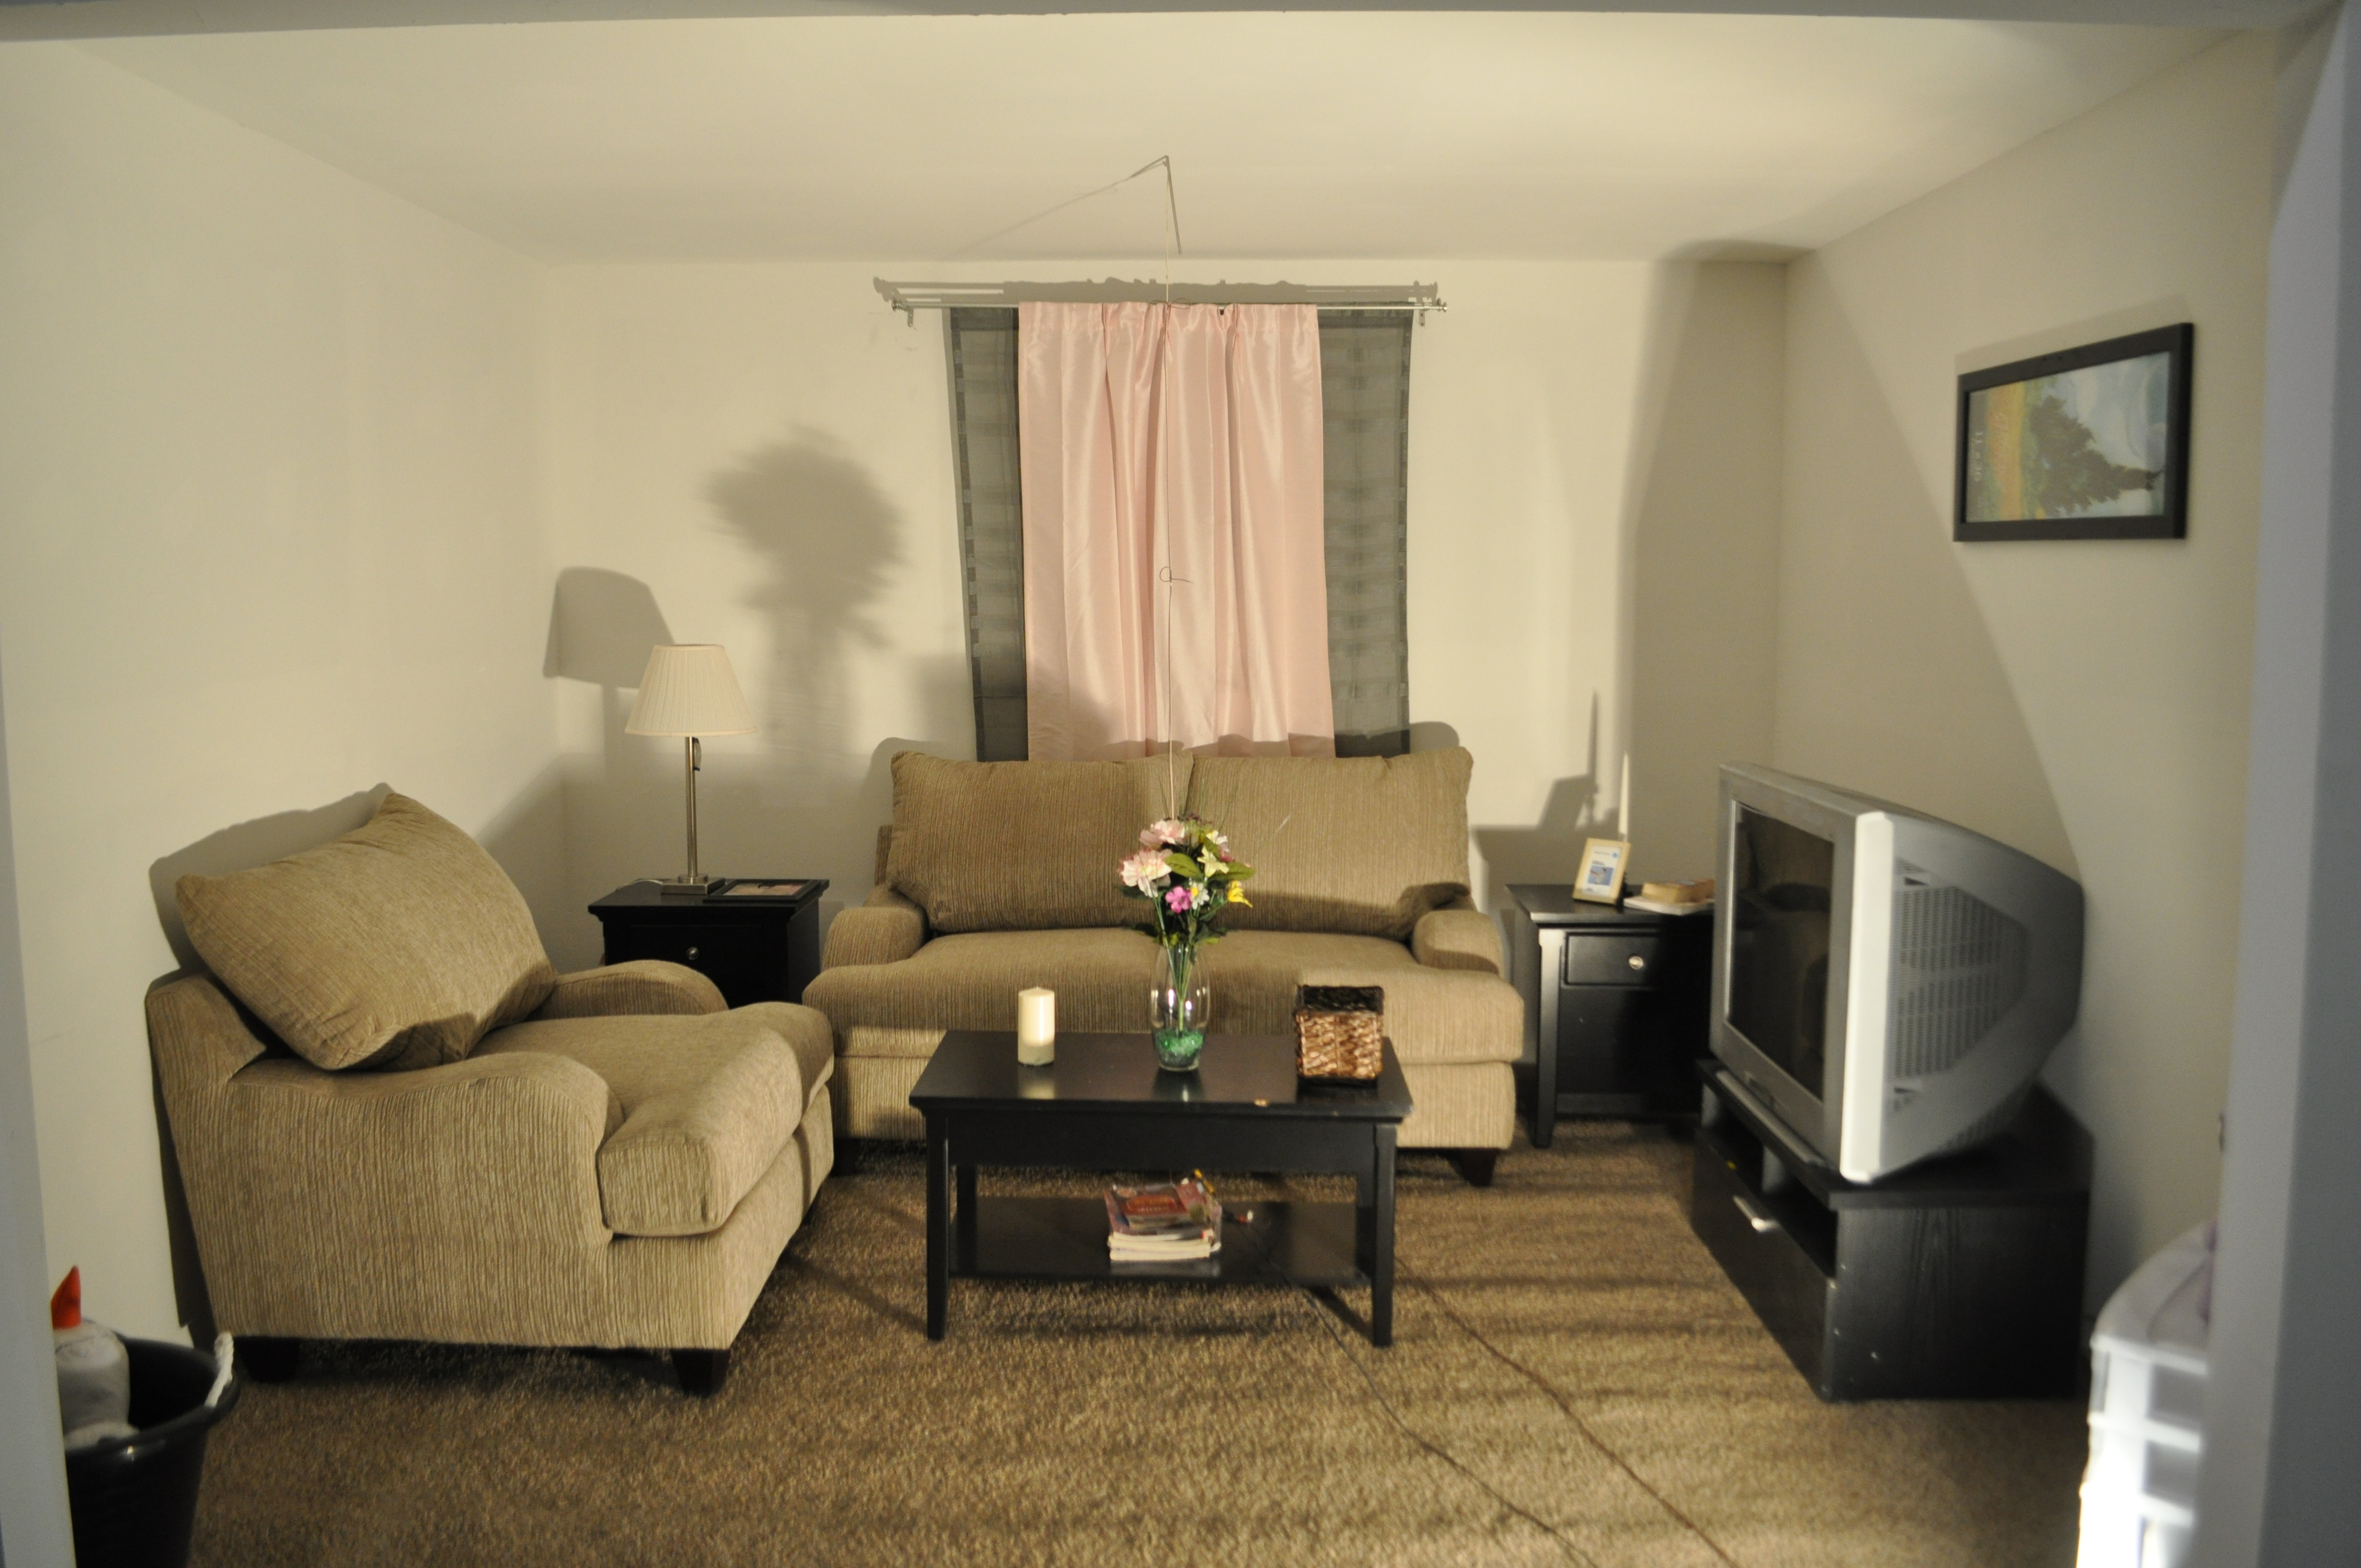
\includegraphics[width=5cm]{0_Images/Vent_Limited_Room/Furnished_Overall.jpg}} &
	\subfloat[]{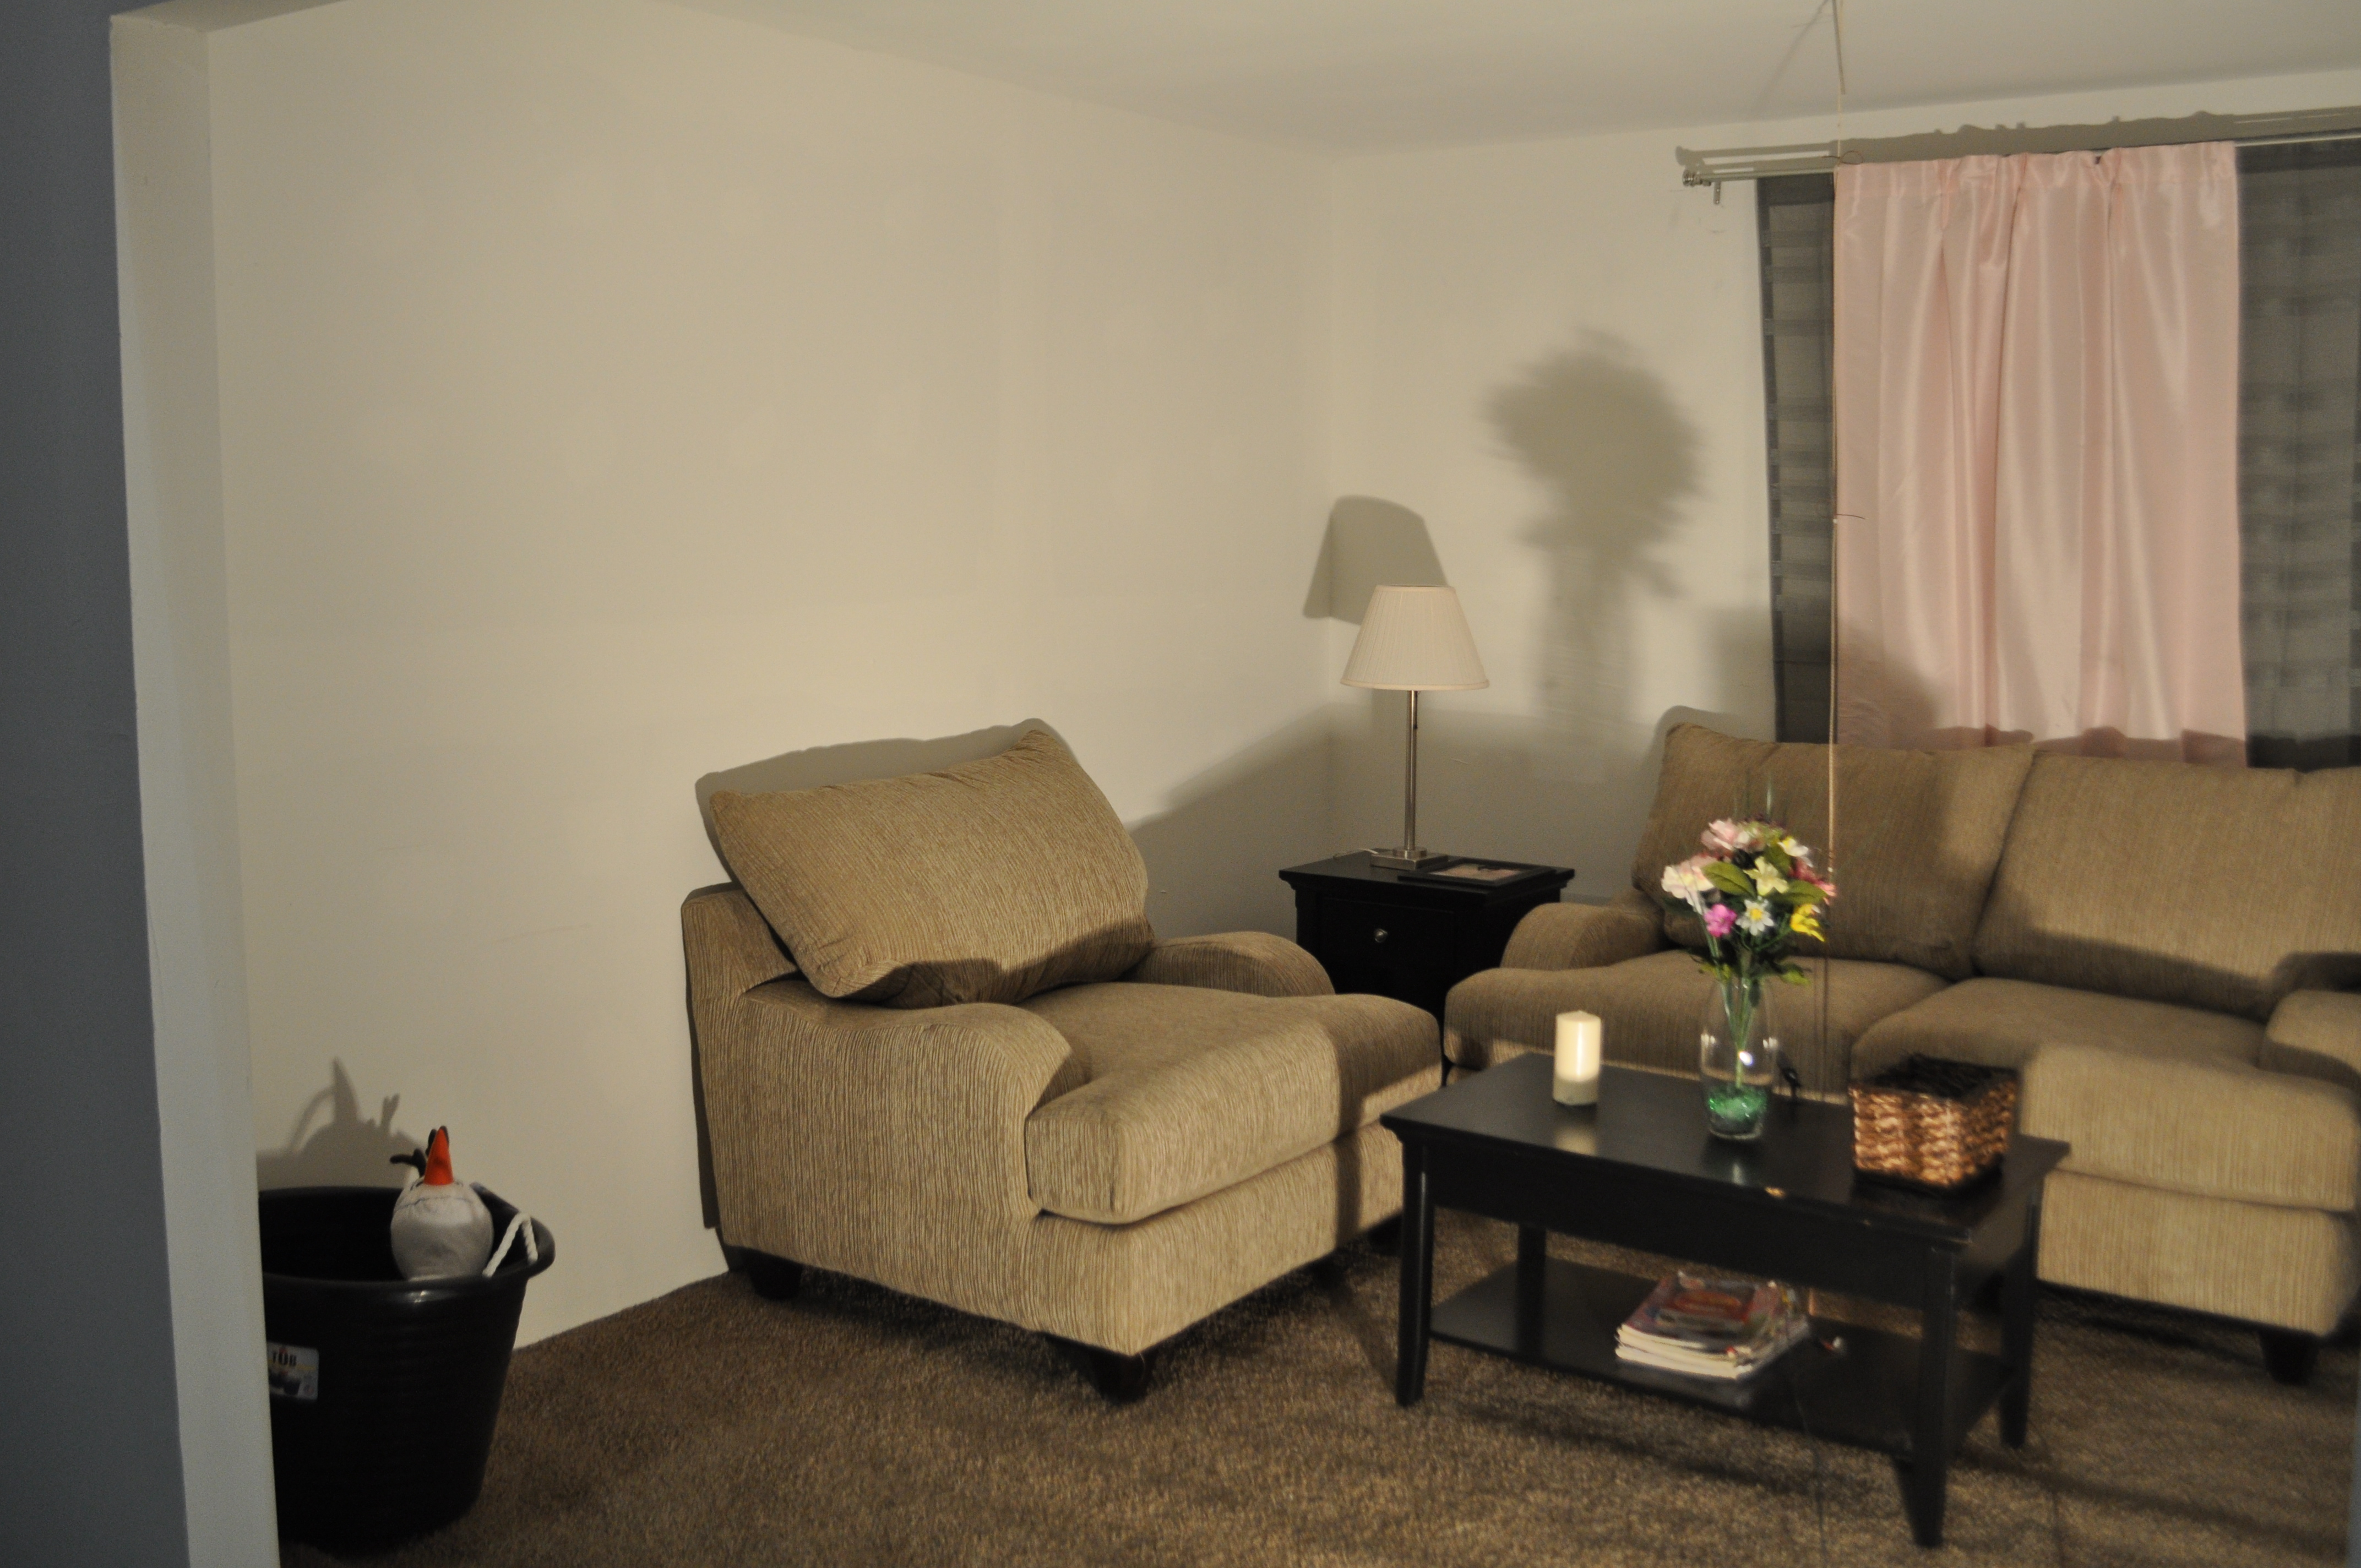
\includegraphics[width=5cm]{0_Images/Vent_Limited_Room/Furnished_Left_Side.jpg}} &
	\subfloat[]{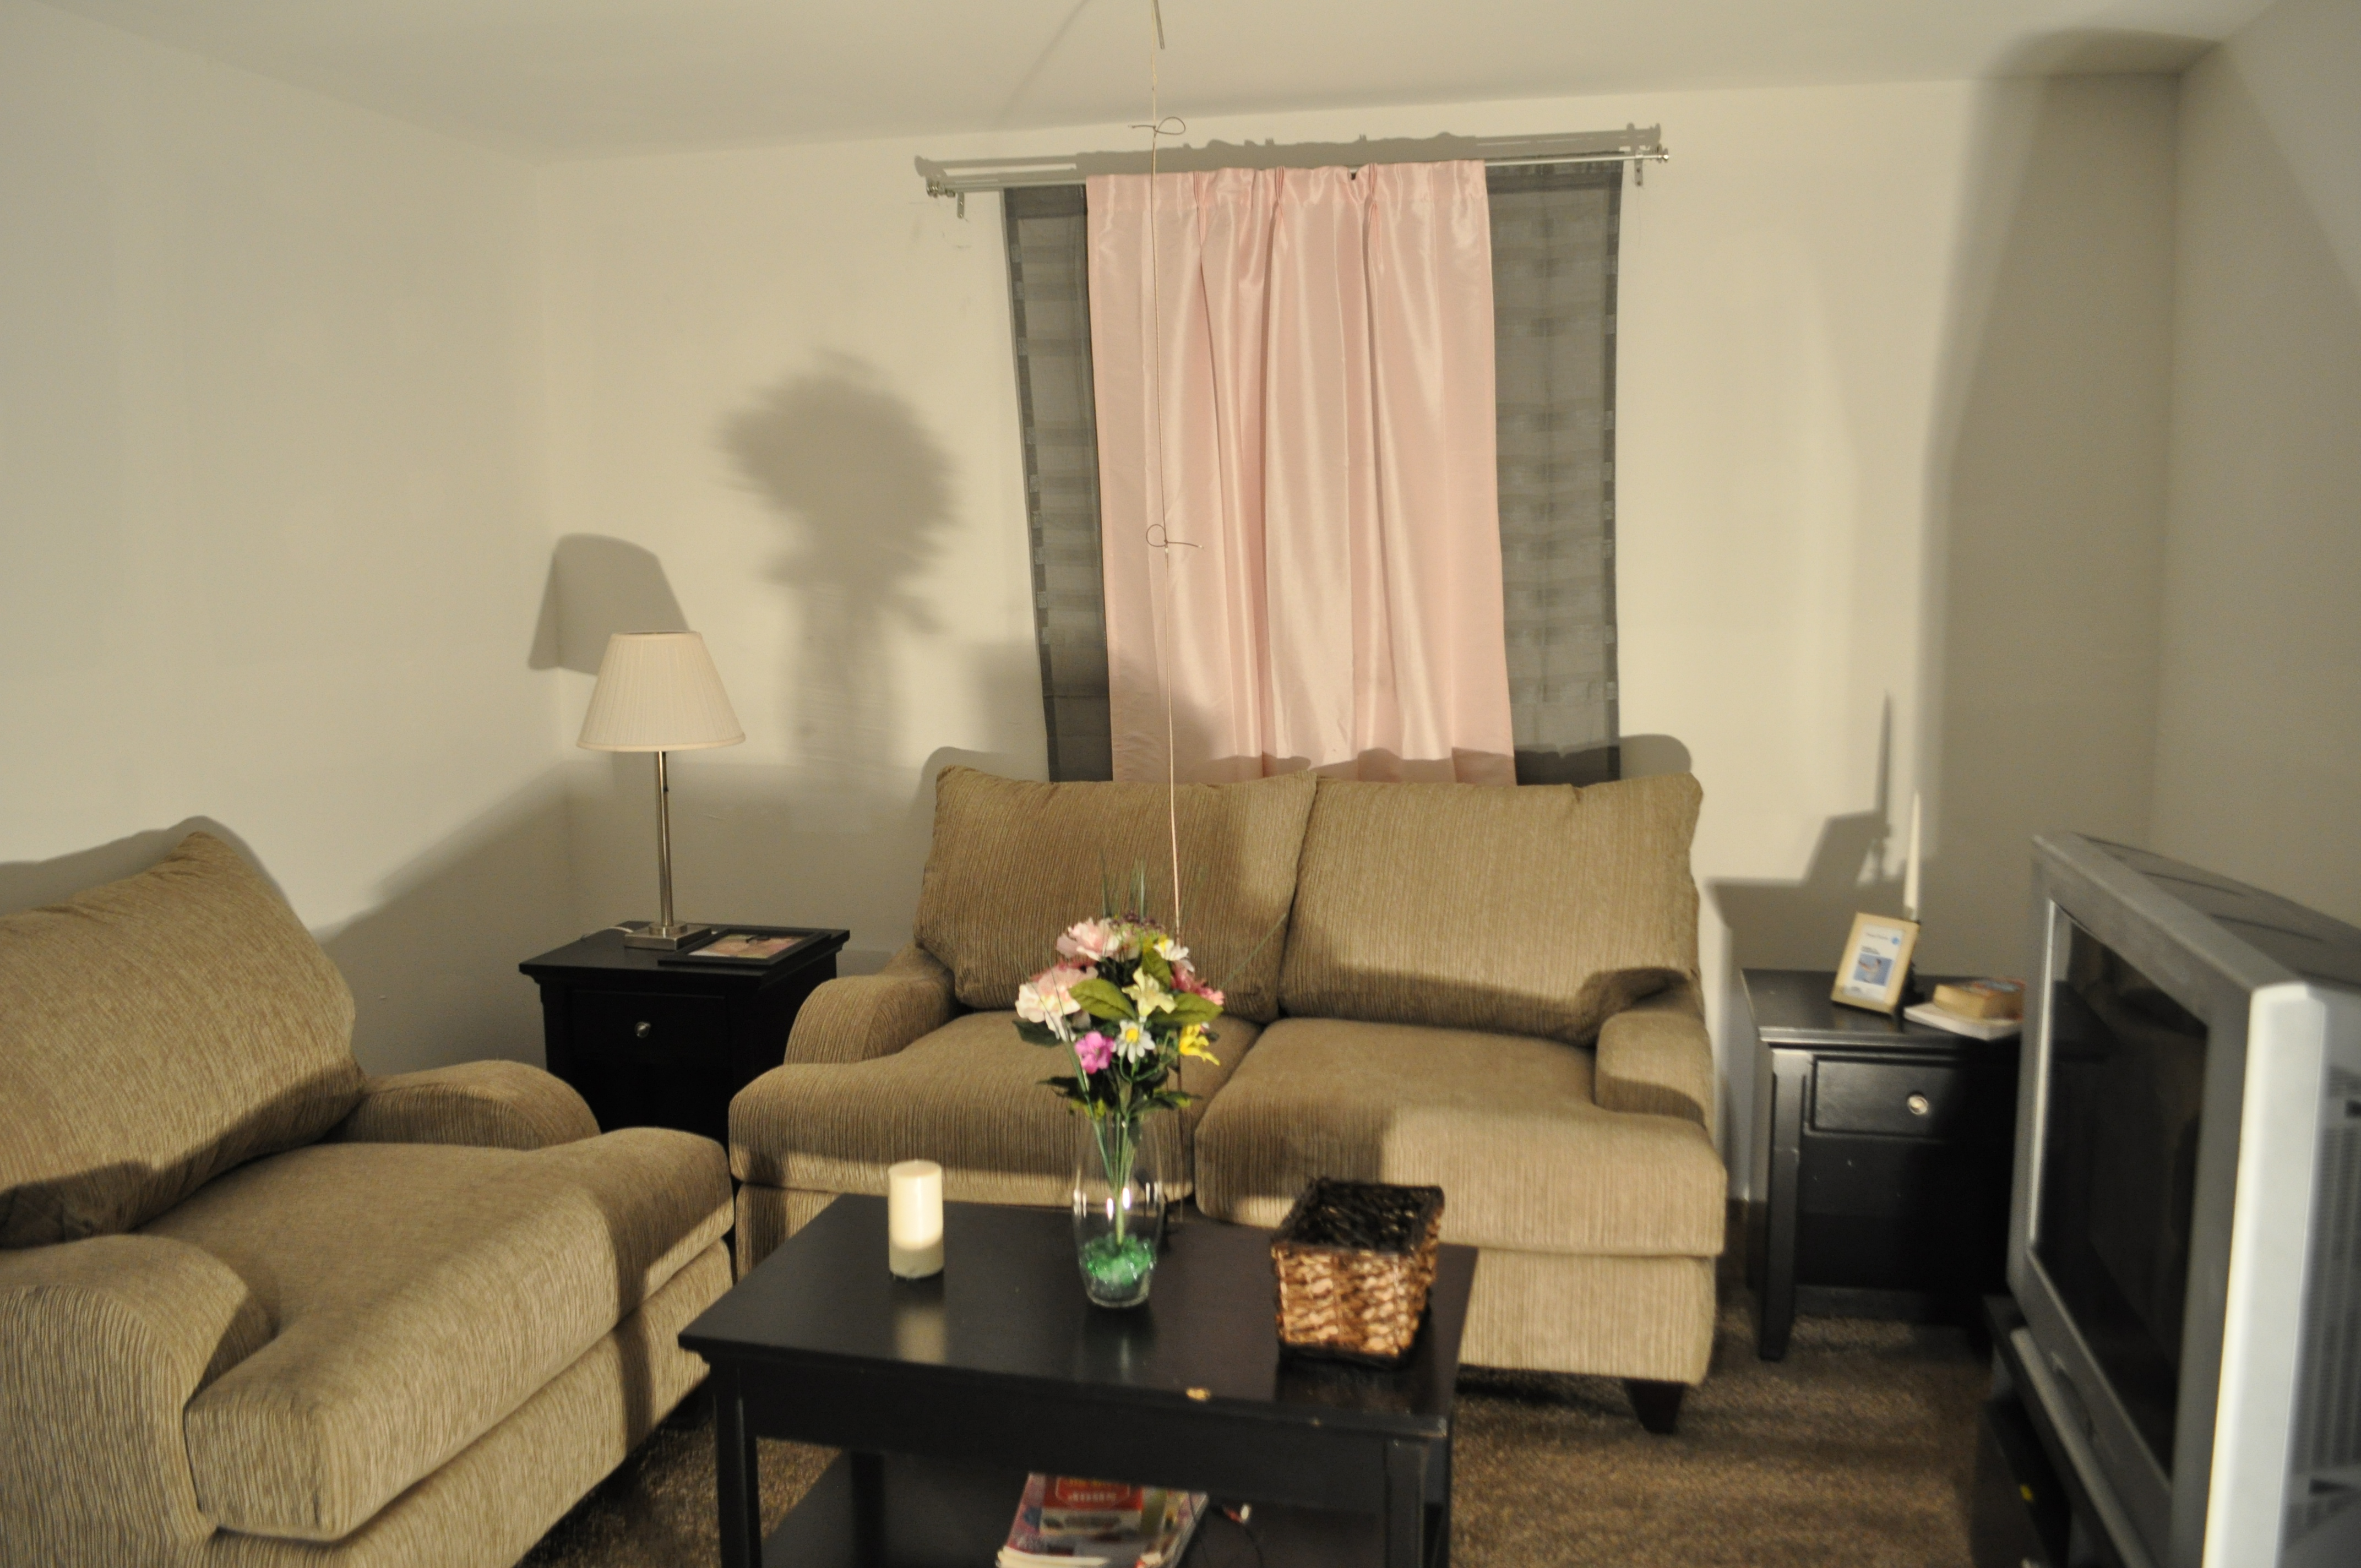
\includegraphics[width=5cm]{0_Images/Vent_Limited_Room/Furnished_Center.jpg}} \\
	\end{tabular}
	\begin{tabular} { c c }
	\subfloat[]{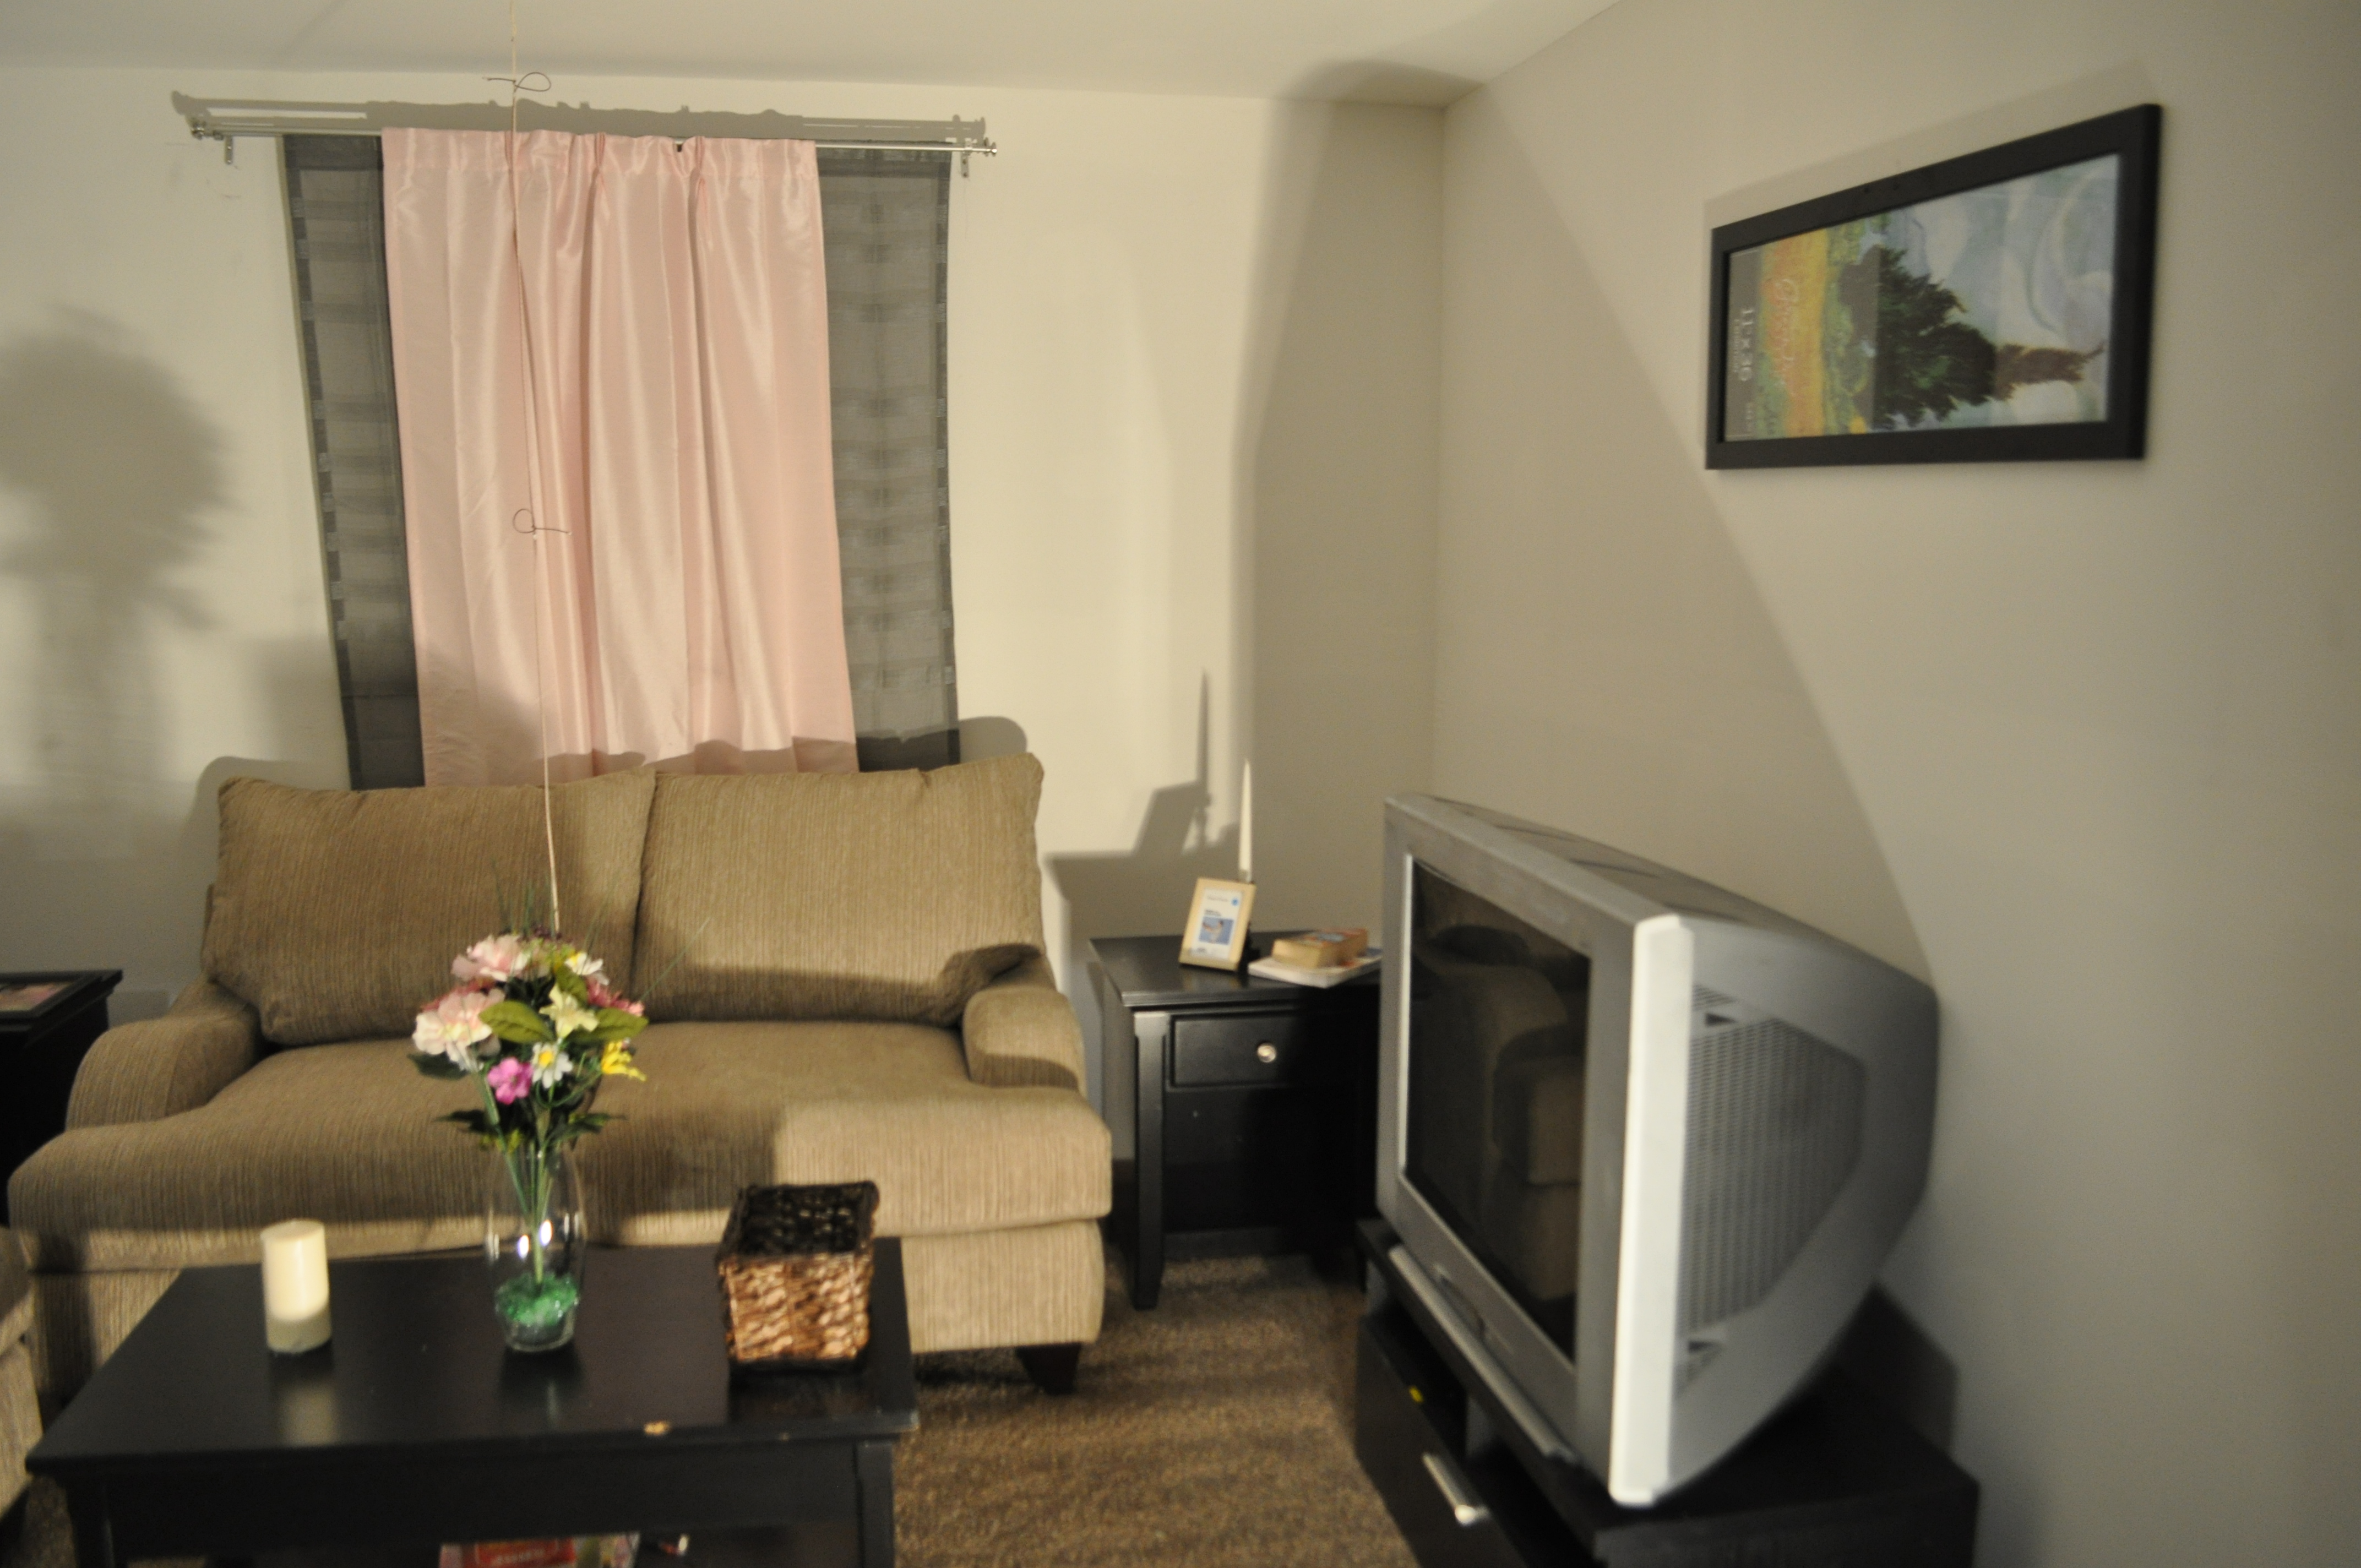
\includegraphics[width=5cm]{0_Images/Vent_Limited_Room/Furnished_Center_Right.jpg}} &
	\subfloat[]{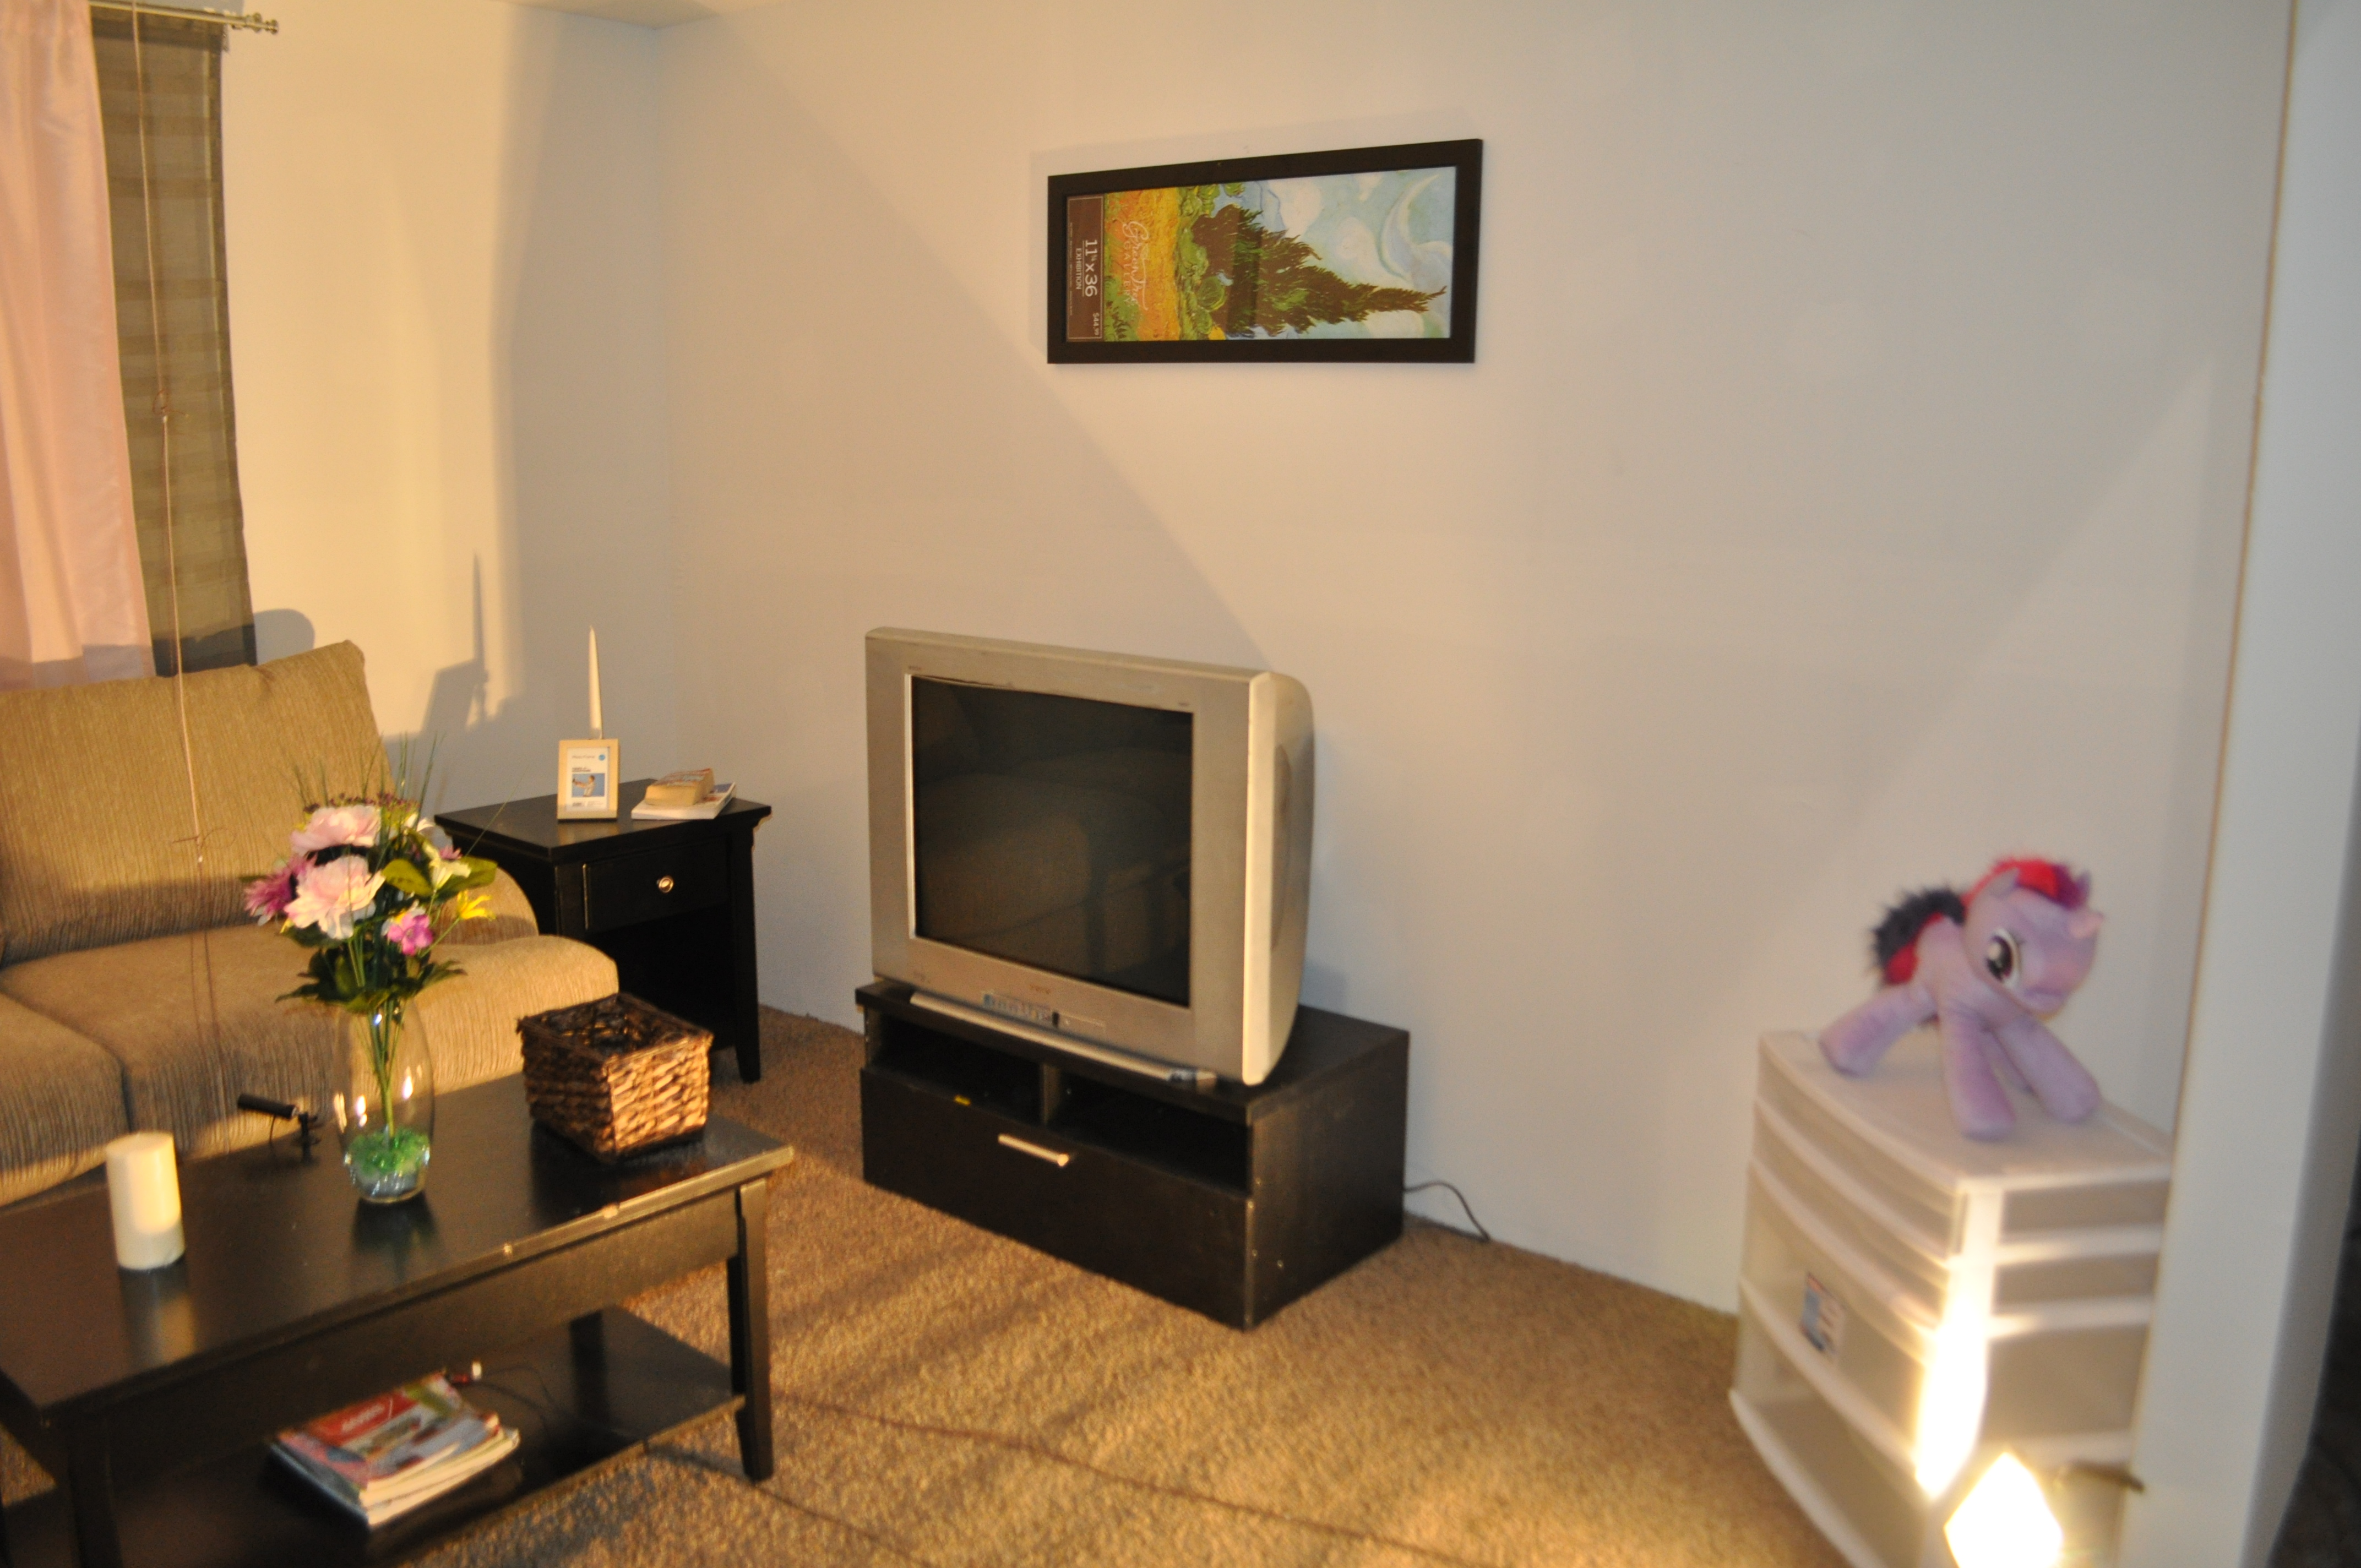
\includegraphics[width=5cm]{0_Images/Vent_Limited_Room/Furnished_Right_Side.jpg}} \\
	\end{tabular}
	\caption{Furnished Room Images}
	\label{fig:furnished_images}
\end{figure}

\begin{figure}[H]
	\centering
	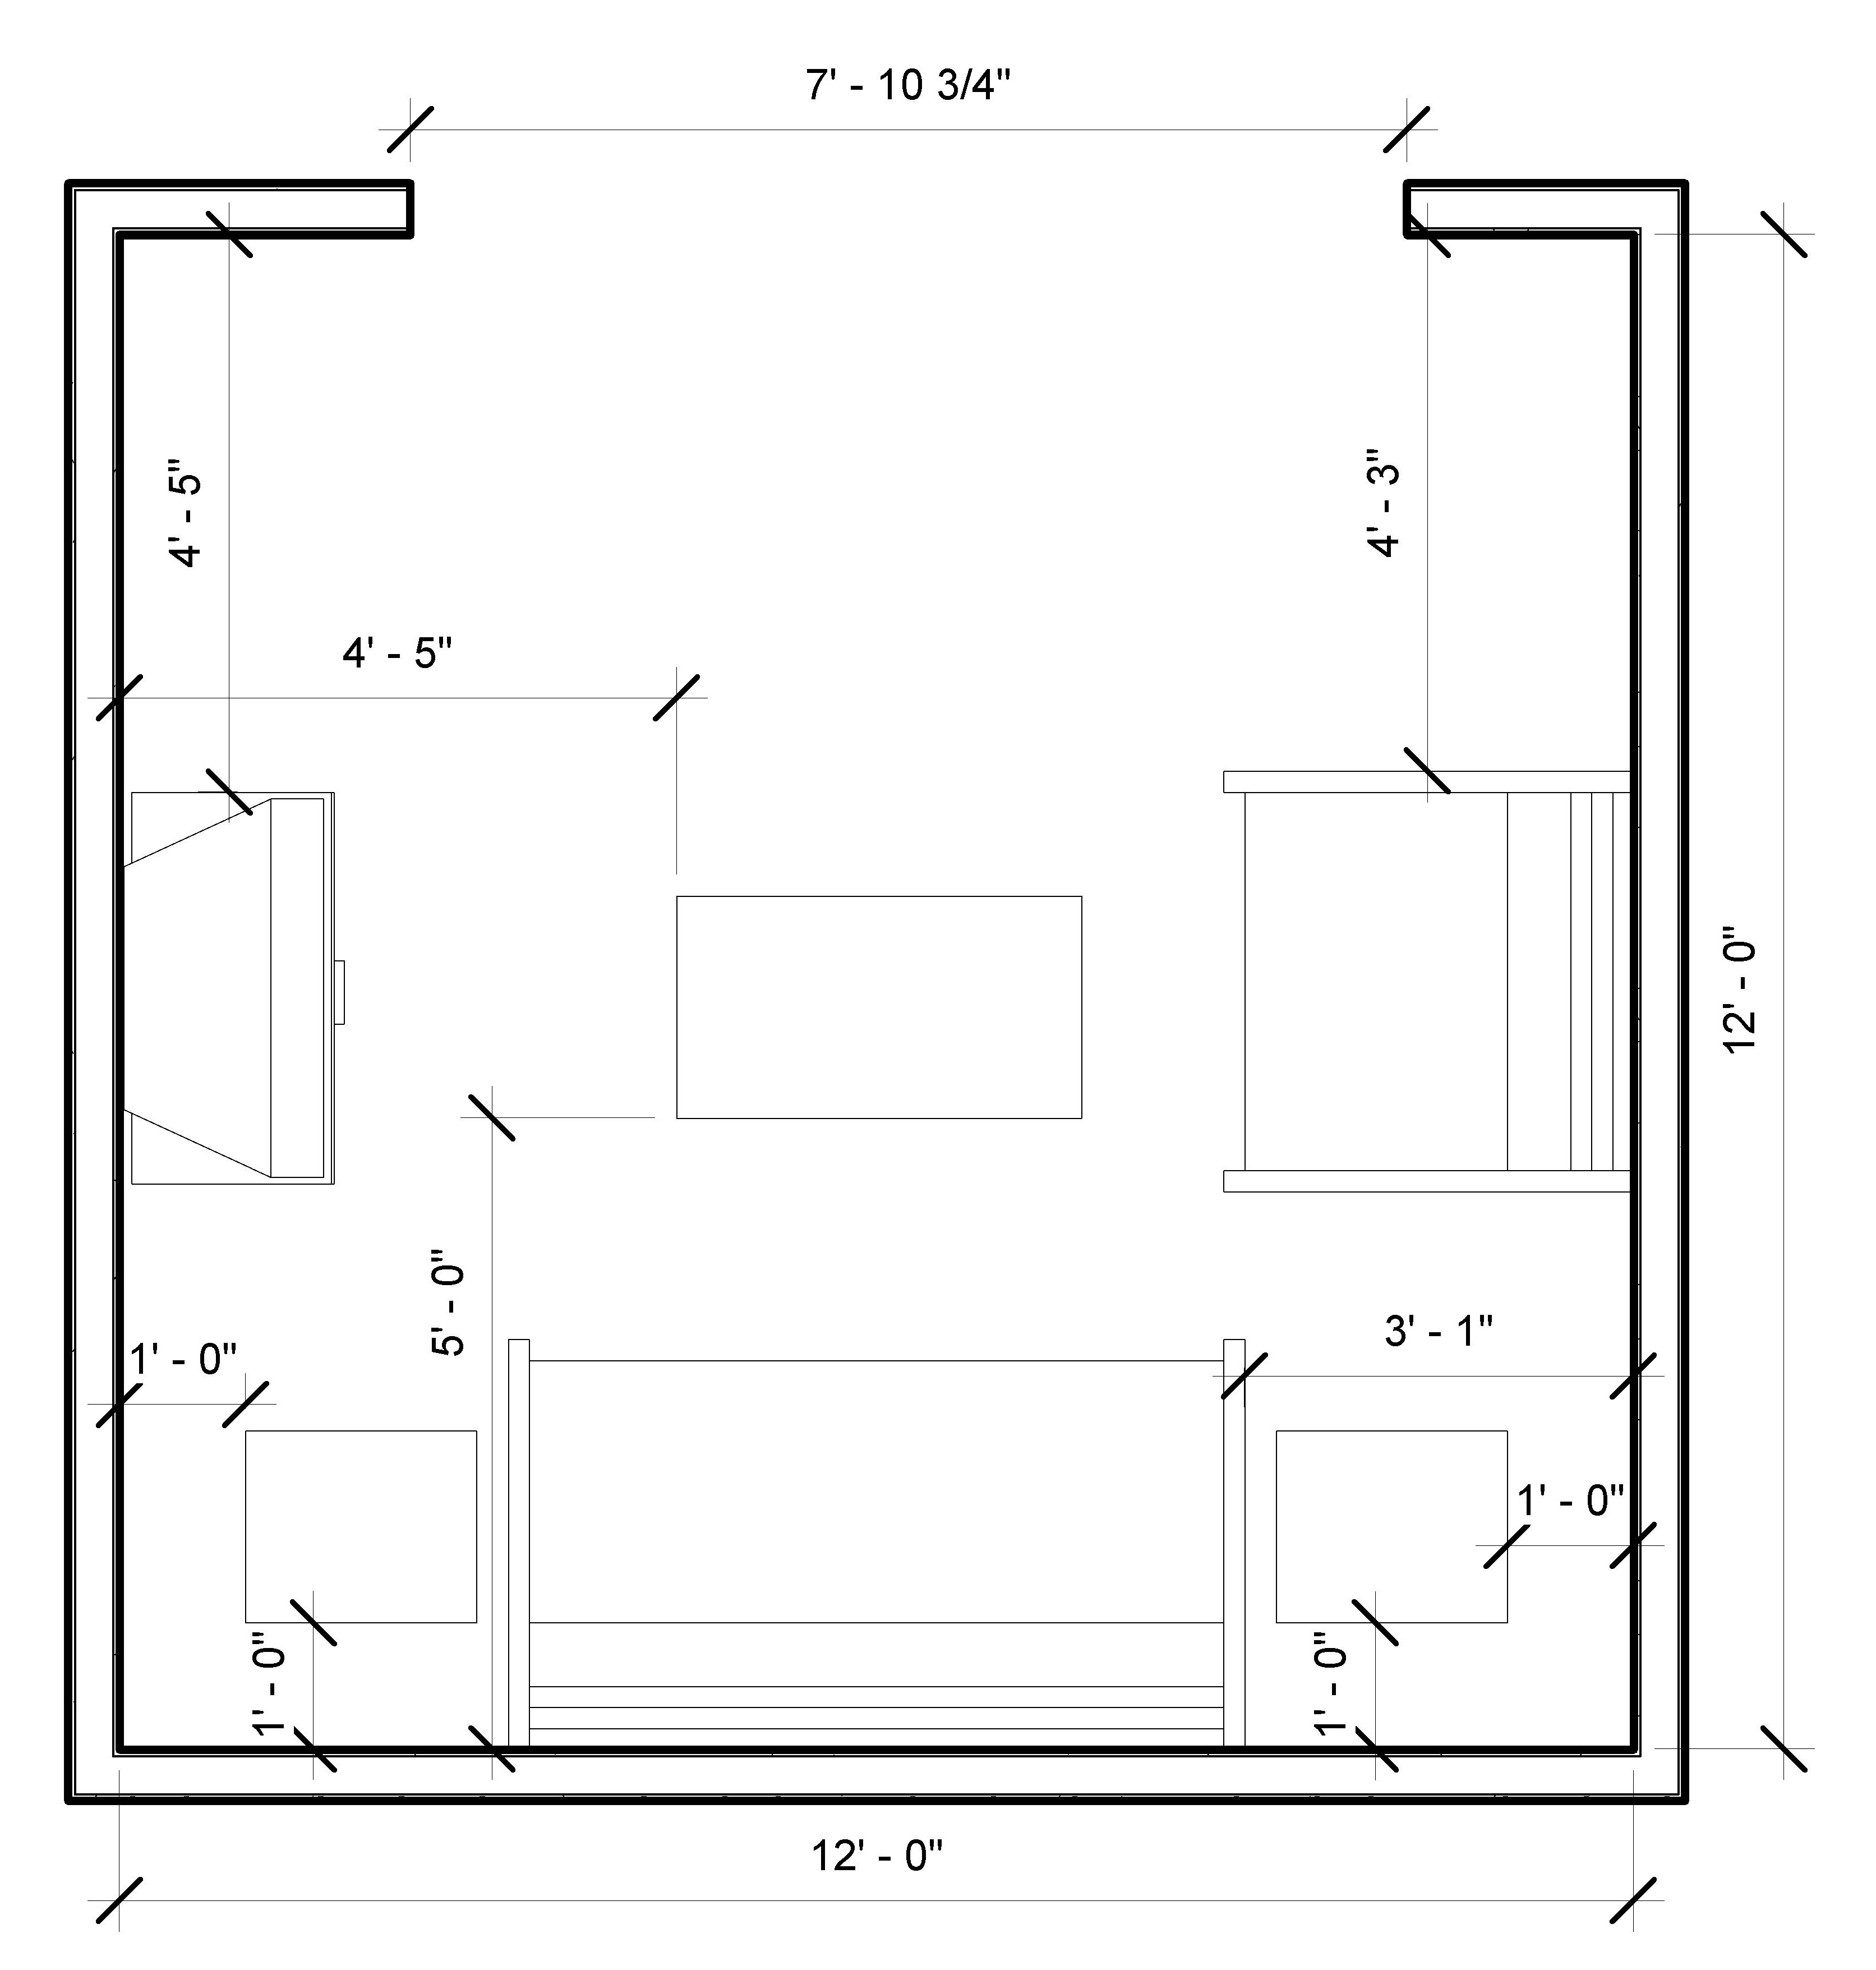
\includegraphics[width=3in]{0_Images/Vent_Limited_Room/Furnished_Room.jpg}
	\caption{Furnished Room Layout}
	\label{fig:furnished_layout}
\end{figure}

Ignition for the furnished compartment occurred in the back left corner of the couch up against the arm using a standard flame \hl{from british furniture standards}. The room was permitted to burn completely out over a duration of 12 minutes and 45 seconds. Figure \ref{fig:furnished_screenshots}  shows the experiment results every 30 seconds up until flash over and then in one minute increments following flash over. 


\begin{figure}[H]
	\centering
	\begin{tabular} {c c c}
		\subfloat[00:00]{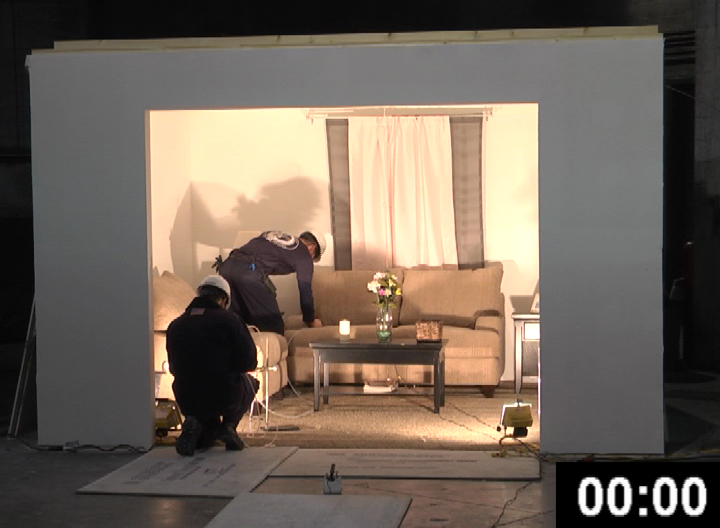
\includegraphics[width=3.9cm]{0_Images/Vent_Limited_Room/furnished_screenshot(1).png}} &
		\subfloat[00:30]{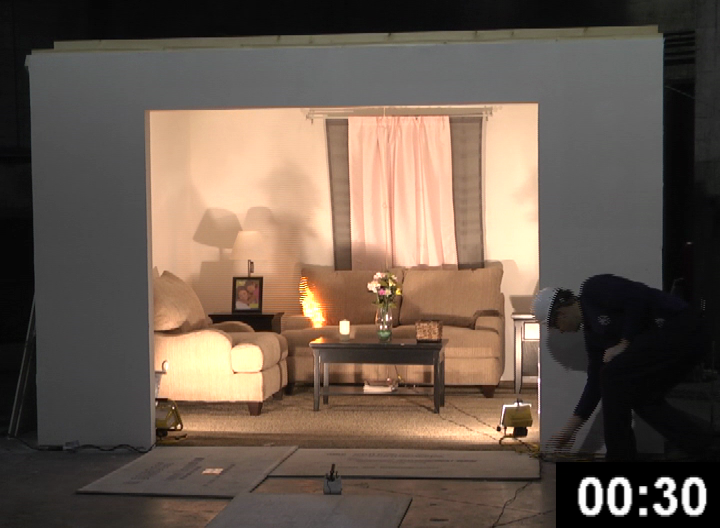
\includegraphics[width=3.9cm]{0_Images/Vent_Limited_Room/furnished_screenshot(2).png}} &
		\subfloat[01:00]{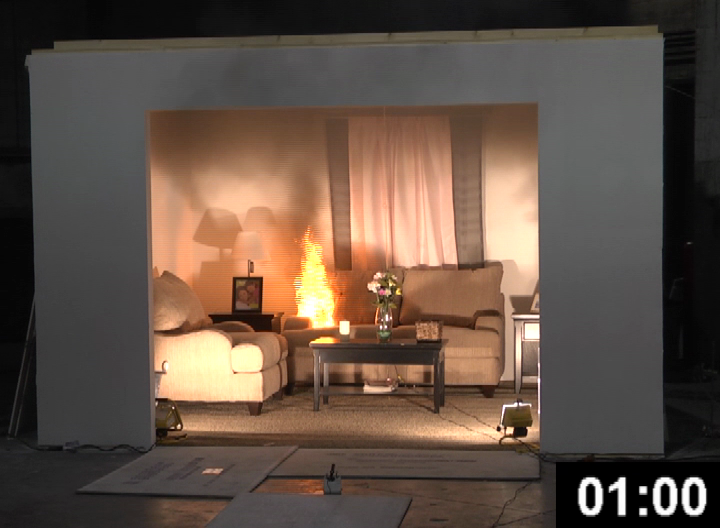
\includegraphics[width=3.9cm]{0_Images/Vent_Limited_Room/furnished_screenshot(3).png}} \\
		\subfloat[01:30]{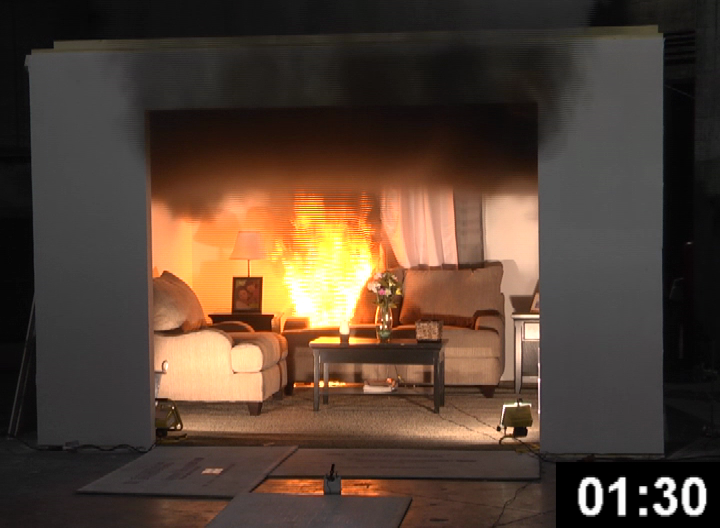
\includegraphics[width=3.9cm]{0_Images/Vent_Limited_Room/furnished_screenshot(4).png}} &
		\subfloat[02:00]{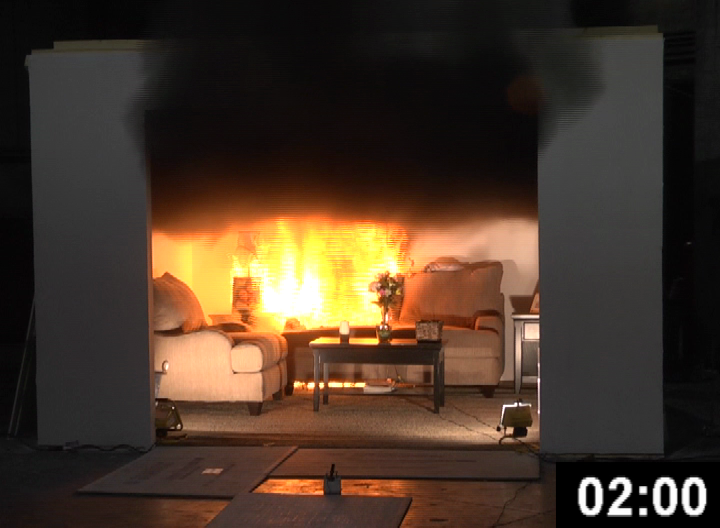
\includegraphics[width=3.9cm]{0_Images/Vent_Limited_Room/furnished_screenshot(5).png}} &
		\subfloat[02:30]{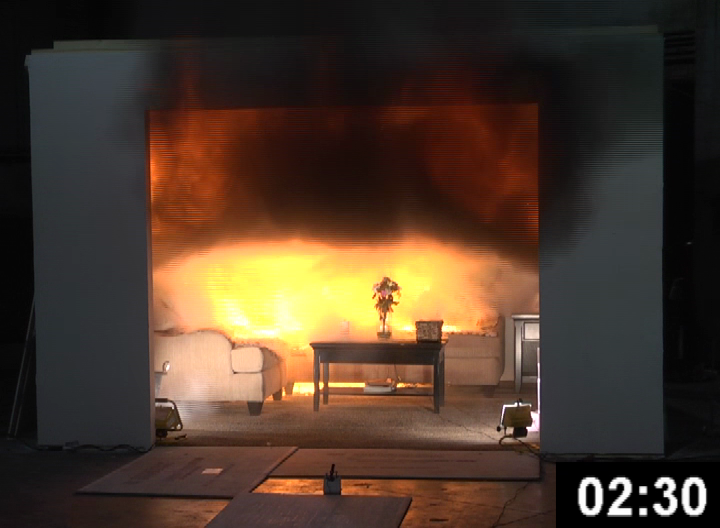
\includegraphics[width=3.9cm]{0_Images/Vent_Limited_Room/furnished_screenshot(6).png}} \\
		\subfloat[02:45]{\includegraphics[width=3.9cm]{0_Images/Vent_Limited_Room/furnished_screenshot(7).png}} &
		\subfloat[03:00]{\includegraphics[width=3.9cm]{0_Images/Vent_Limited_Room/furnished_screenshot(8).png}} &
		\subfloat[04:00]{\includegraphics[width=3.9cm]{0_Images/Vent_Limited_Room/furnished_screenshot(10).png}} \\
		\subfloat[05:00]{\includegraphics[width=3.9cm]{0_Images/Vent_Limited_Room/furnished_screenshot(11).png}} &
		\subfloat[06:00]{\includegraphics[width=3.9cm]{0_Images/Vent_Limited_Room/furnished_screenshot(12).png}} &
		\subfloat[07:00]{\includegraphics[width=3.9cm]{0_Images/Vent_Limited_Room/furnished_screenshot(13).png}} \\
		\subfloat[08:00]{\includegraphics[width=3.9cm]{0_Images/Vent_Limited_Room/furnished_screenshot(14).png}} &
		\subfloat[09:00]{\includegraphics[width=3.9cm]{0_Images/Vent_Limited_Room/furnished_screenshot(15).png}} &
		\subfloat[10:00]{\includegraphics[width=3.9cm]{0_Images/Vent_Limited_Room/furnished_screenshot(16).png}} \\
	\end{tabular}
	
	\begin{tabular}{c c}
		\subfloat[11:00]{\includegraphics[width=3.9cm]{0_Images/Vent_Limited_Room/furnished_screenshot(17).png}} &
		\subfloat[12:00]{\includegraphics[width=3.9cm]{0_Images/Vent_Limited_Room/furnished_screenshot(18).png}} \\	
	\end{tabular}
	
	\caption{Furnished Room Experiment Images}
	\label{fig:furnished_screenshots}
\end{figure}

\paragraph{Over Furnished Compartment} \mbox{}

The over furnished compartment contained six stuffed brown chairs, two orange sleeper sofas and two one green sleeper sofa from the furniture aquired for the full scale fire experiments. The furniture was arranged as shown in Figure \ref{fig:horder_images} with dimensions shown in Figure \ref{fig:horder_layout}.

\begin{figure}[H]
	\centering
	\begin{tabular} {c c c}
		\subfloat[]{\includegraphics[width=5cm]{0_Images/Vent_Limited_Room/Horder1.jpg}} &
		\subfloat[]{\includegraphics[width=5cm]{0_Images/Vent_Limited_Room/Horder2.jpg}} &
		\subfloat[]{\includegraphics[width=5cm]{0_Images/Vent_Limited_Room/Horder3.jpg}} \\
	\end{tabular}
	\caption{Over Furnished Compartment}
	\label{fig:horder_images}
\end{figure}

\begin{figure}[H]
	\centering
	\includegraphics[width=5in]{0_Images/Vent_Limited_Room/HorderRoom.jpg}
	\caption{Over Furnished Compartment Layout}
	\label{fig:horder_layout}
\end{figure}

The over furnished room was ignited in the \hl{Where did this get ignited?} and permitted to burn until a portion of the ceiling failed due to the fire in the compartment at 10 minutes and 10 seconds followed by an entire sheet of gypsum failing off the ceiling at 11 minutes and 30 seconds at which time the fire was extinguished. Figure \ref{fig:horder_screenshots} shows the the experiment every 1 minute along with 5 seconds after the first instance of ceiling failure at 10 minutes 15 seconds and again at 11 minutes and 37 seconds following the second failure.

\begin{figure}[H]
	\centering
	\begin{tabular} {c c c}
		\subfloat[00:00]{\includegraphics[width=3.9cm]{0_Images/Vent_Limited_Room/horder(1).png}} &
		\subfloat[01:00]{\includegraphics[width=3.9cm]{0_Images/Vent_Limited_Room/horder(2).png}} &
		\subfloat[02:00]{\includegraphics[width=3.9cm]{0_Images/Vent_Limited_Room/horder(3).png}} \\
		\subfloat[03:00]{\includegraphics[width=3.9cm]{0_Images/Vent_Limited_Room/horder(4).png}} &
		\subfloat[04:00]{\includegraphics[width=3.9cm]{0_Images/Vent_Limited_Room/horder(5).png}} &
		\subfloat[05:30]{\includegraphics[width=3.9cm]{0_Images/Vent_Limited_Room/horder(6).png}} \\
		\subfloat[06:00]{\includegraphics[width=3.9cm]{0_Images/Vent_Limited_Room/horder(7).png}} &
		\subfloat[07:00]{\includegraphics[width=3.9cm]{0_Images/Vent_Limited_Room/horder(8).png}} &
		\subfloat[08:00]{\includegraphics[width=3.9cm]{0_Images/Vent_Limited_Room/horder(9).png}} \\
		\subfloat[09:00]{\includegraphics[width=3.9cm]{0_Images/Vent_Limited_Room/horder(10).png}} &
		\subfloat[10:00]{\includegraphics[width=3.9cm]{0_Images/Vent_Limited_Room/horder(11).png}} &
		\subfloat[10:15]{\includegraphics[width=3.9cm]{0_Images/Vent_Limited_Room/horder(11a).png}} \\
	\end{tabular}
	
	\begin{tabular}{c c}
		\subfloat[11:00]{\includegraphics[width=3.9cm]{0_Images/Vent_Limited_Room/horder(12).png}} &
		\subfloat[11:37]{\includegraphics[width=3.9cm]{0_Images/Vent_Limited_Room/horder(13).png}} \\	
	\end{tabular}
	
	\caption{Overstuffed Room Experiment Images}
	\label{fig:horder_screenshots}
\end{figure}

\paragraph{Compartment Burn Results} \mbox{}

In each of the compartment burns the total heat release rate versus time was recorded via the oxygen consumption calorimeter. Although the compartment geometry was identical the fuel load was significantly different leading to two very different growth rates. As seen in Table \ref{table:comp_burn_results}, the furnished room reached its fully developed heat release rate at 2 minutes and 56 seconds where the over furnished room took longer to grow reaching its fully developed stage at 5 minutes and 46 seconds. The fully develop stage for both rooms was approximately 6500kW until the failure of the ceiling in the over furnished compartment failed increasing the available oxygen and thus the the heat release rate as seen in Figure \ref{fig:comp_burn_chart}. 

The difference in the fuel configuration was the time the compartment spent in its fully developed stage as shown in Figure \ref{fig:comp_burn_chart}. The furnished compartment reached a fully developed stage within 3 minutes of ignition and maintained that heat release rate for 3 minutes before it began to decay at 6 minutes. The over furnished compartment reached a similar peak heat release rate at just under 6 minutes and maintained that through the failure of the ceiling at 10 minutes at which time it increased. The over furnished compartment had more fuel to consume thus it remained fully developed much longer than the furnished compartment. 

This demonstrates how heat release rate or energy release rate in a compartment fire is limited by the available oxygen for combustion. Additional fuel does not necessarily mean additional energy release per unit time, however it does mean additional energy release over the duration of the fire. This is seen with the total heat release for the furnished compartment being approximately 2500MJ. where the total heat release for the over furnished compartment was approximately 3500MJ and it had yet to enter a fuel limited decay stage. The furnished compartment has entered its fuel limited decay stage as seen in Figure \ref{fig:furnished_screenshots}. The over furnished compartment results from Figure \ref{fig:horder_screenshots} shows there is still a substantial amount of fuel remaining at the time of ceiling failure. 

\begin{table}[H]
	\caption{Compartment Burn Results}
	\begin{tabular}{|c|c|c|}
		\hline
		\textbf{Experiment} & \textbf{Time to Fully Developed} & \textbf{Average Fully Developed HRR (kW)} \\ \hline \hline
		Furnished Room & 02:56 & 6458 \\ \hline
		Over Furnished Room & 05:46 & 6779 \\ \hline
	\end{tabular}
	\label{table:comp_burn_results}
\end{table}

\begin{figure}[H]
	\centering
	\includegraphics[width=5in]{0_Images/Vent_Limited_Room/Compartment_Burn_Chart.pdf}
	\caption{Compartment Burn Results}
	\label{fig:comp_burn_chart}
\end{figure}

\section{Cold Flow Experiments}
To aid in the understanding of air flow with a residential structure when using positive pressure attack and positive pressure ventilation cold flow experiments were conducted. The results of the cold flow experiments were used by the project technical panel to select a single fan to be used in the full scale fire experiments. A total of 24 experiments were run using six different fans provided by Leader, RamFan, SuperVac, Tempest, UniFire and Ventry. Each manufacture graciously provided the use of one 18" electric and the comparable 18" electric fan. Table \ref{table:cold_flow_Fans} shows the fans tested, manufacturer and model number. 

\begin{table}[H]
	\centering
	\caption{Fans Used in Cold Flow Experiments}
	\begin{tabular}{|c|c|c|}
		\hline
		Manufacturer & Drive Method (Electric or Gas) & Model Number \\ \hline \hline
		Leader & Gas & MT236 \\ \hline
		Leader & Electric & EDS 230 \\ \hline
		Ramfan & Gas & GX350 \\ \hline
		Ramfan & Electric & EX500 \\ \hline
		Super Vac & Gas & 718G4-H \\ \hline
		Super Vac & Electric & 718VR3 \\ \hline
		Tempest & Gas & BD-18-H-5.5 \\ \hline
		Tempest & Electric & VS-18-R-2.0 \\ \hline
		Unifire & Gas & DST-3P4 \\ \hline
		Unifire & Electric & EB18SP \\ \hline
		Ventry & Gas & 20GX160 \\ \hline
		Ventry & Electric & 20E1.5GFCI \\ \hline
	\end{tabular}
	\label{table:cold_flow_Fans}
\end{table}

This report is not intended to identify the pros and cons of a particular fan or manufacturer thus results will be presented in a generic fashion leaving the identifying characteristics of the fans out of the results. 

\subsection{Single Story Cold Flow Experiments}
The single story structure was instrumented with air flow and pressure sensors to evaluate the flow and pressure capabilities of each fan tested. The front, bedroom 2, bedroom 3, and master bedroom doorways were instrumented with five bi-directional probes arrayed vertically along the center line at 8in, 24in, 30in, 46in and 62in above the floor. In addition the living room, master bedroom, bedroom 2 and bedroom 3 windows were instrumented with five bi-directional probes arrayed vertically along the center line at 6in, 18in, 30in, 42in and 54in above the window sill. Pressure was recorded through a differential pressure transducer in the Living Room, Dining Room, Kitchen, Master Bedroom, Bedroom 2 and Bedroom 3 at 12in, 48in and 84in above the floor. The locations of each sensor is shown in Figure \ref{fig:SingleStoryColdFlowSensors}. 

\begin{figure} [H]
	\centering
	\includegraphics[width = 5in]{0_Images/ColdFlow/SingleStory_Sensors.png}
	\caption{Single Story Cold Flow Sensors}
	\label{fig:SingleStoryColdFlowSensors}
\end{figure}

Each of the six electric and six gas fans were tested in the single story structure with 11 different exhaust configurations. Each configuration was tested for 2.5minutes to allow flows and pressures to stabilize. Figure \ref{fig:ColdFlowConfig_SingleStory} shows the 11 configurations graphically which are also described in Table \ref{tab:ColdFlowConfig_SingleStory} with inlet/exhaust dimensions and the overall ratio of outlet to inlet size. 

\begin{figure}[H]
	\centering
	\begin{tabular}{c c c}
		\subfloat[Congfiguration 1]{\includegraphics[width = 1.5in]{0_Images/ColdFlow/Configurations/One_Story/Experiment_1.jpg}} & 
		\subfloat[Congfiguration 2]{\includegraphics[width = 1.5in]{0_Images/ColdFlow/Configurations/One_Story/Experiment_2.jpg}} & 
		\subfloat[Congfiguration 3]{\includegraphics[width = 1.5in]{0_Images/ColdFlow/Configurations/One_Story/Experiment_3.jpg}} \\
		\subfloat[Congfiguration 4]{\includegraphics[width = 1.5in]{0_Images/ColdFlow/Configurations/One_Story/Experiment_4.jpg}} & 
		\subfloat[Congfiguration 5]{\includegraphics[width = 1.5in]{0_Images/ColdFlow/Configurations/One_Story/Experiment_5.jpg}} & 
		\subfloat[Congfiguration 6]{\includegraphics[width = 1.5in]{0_Images/ColdFlow/Configurations/One_Story/Experiment_6.jpg}} \\
		\subfloat[Congfiguration 7]{\includegraphics[width = 1.5in]{0_Images/ColdFlow/Configurations/One_Story/Experiment_7.jpg}} & 
		\subfloat[Congfiguration 8]{\includegraphics[width = 1.5in]{0_Images/ColdFlow/Configurations/One_Story/Experiment_8.jpg}} & 
		\subfloat[Congfiguration 9]{\includegraphics[width = 1.5in]{0_Images/ColdFlow/Configurations/One_Story/Experiment_9.jpg}} \\
	\end{tabular}
	\begin{tabular}{c c}
		\subfloat[Congfiguration 10]{\includegraphics[width = 1.5in]{0_Images/ColdFlow/Configurations/One_Story/Experiment_10.jpg}} & 
		\subfloat[Congfiguration 11]{\includegraphics[width = 1.5in]{0_Images/ColdFlow/Configurations/One_Story/Experiment_11.jpg}} \\
	\end{tabular}
	\label{fig:ColdFlowConfig_SingleStory}
	\caption{Cold Flow Ventilation Configurations - Single Story}
\end{figure}

\begin{table} [H]
	\caption{Cold Flow Ventilation Configurations - Single Story}
	\begin{tabular}{|c|c|c|c|c|}
		\hline
		Configuration & Inlet Size (ft$^2$) & Open Windows & Exhaust Size (ft$^2$) & Exhaust to Inlet Ratio \\ \hline \hline
		1 & 0 & - & 0 & - \\ \hline
		2 & 20 & - & 0 & 0:1 \\ \hline
		3 & 20 & Living & 45 & 2.3:1 \\ \hline
		4 & 20 & Living, Bed 2 & 60 & 3.0:1 \\ \hline
		5 & 20 & Bed 2 & 15 & 0.8:1 \\ \hline
		6 & 20 & 1/2 Bed 2 & 7.5 & 0.4:1 \\ \hline
		*7 & 20 & Bed 2 & 15 & 0.8:1 \\ \hline
		8 & 20 & Master, Bed 2 Bed 3 & 60 & 3.0:1 \\ \hline
		9 & 20 & Bed 2, Bed 3 & 30 & 1.5:1 \\ \hline
		10 & 20 & Bed 3 & 15 & 0.8:1 \\ \hline
		11 & 20 & Living, Master, Bed 2, Bed 3 & 105 & 5.3:1 \\ \hline
	\end{tabular}
	\begin{tablenotes}
		\item *Fan 1/2 Throttle
	\end{tablenotes}
	\label{tab:ColdFlowConfig_SingleStory}
\end{table}


The results were graphed by opening for flow and room for pressure. The results of all 12 experiments can be found grouped by fan in Appendix XX. 

\subsection{Two Story Cold Flow Experiments}
The two story structure was instrumented with air flow and pressure sensors to evaluate the flow and pressure capabilities of each fan tested. The front, bedroom 3, Kitchen and master bedroom doorways were instrumented with five bi-directional probes arrayed vertically along the center line at 8in, 24in, 30in, 46in and 62in above the floor. In addition the Family Room 1, Family Room 2, and bedroom 3 windows were instrumented with five bi-directional probes arrayed vertically along the center line at 6in, 18in, 30in, 42in and 54in above the window sill. Pressure was recorded through a differential pressure transducer in the Family Room, Foyer, Living Room, Master Bedroom, Bedroom 2, Bedroom 3 and Bedroom 4at 12in, 48in and 84in above the floor. The locations of each sensor is shown in Figure \ref{fig:TwoStoryColdFlowSensors}. 

\begin{figure} [H]
	\centering
	\begin{tabular}{c c}
		\subfloat[First Floor]{\includegraphics[width = 2.5in]{0_Images/ColdFlow/TwoStory_Sensors_1st.png}} &
		\subfloat[First Floor]{\includegraphics[width = 2.5in]{0_Images/ColdFlow/TwoStory_Sensors_2nd.png}} \\
	\end{tabular}
	\caption{Single Story Cold Flow Sensor Locations}
	\label{fig:TwoStoryColdFlowSensors}
\end{figure}

\begin{figure}[H]
	\centering
	\begin{tabular}{c c c c}
		\subfloat[Congfiguration 1]{\includegraphics[width = 1.5in]{0_Images/ColdFlow/Configurations/Two_Story/Experiment_1.png}} & 
		\subfloat[Congfiguration 2]{\includegraphics[width = 1.5in]{0_Images/ColdFlow/Configurations/Two_Story/Experiment_2.png}} & 
		\subfloat[Congfiguration 3]{\includegraphics[width = 1.5in]{0_Images/ColdFlow/Configurations/Two_Story/Experiment_3.png}} &
		\subfloat[Congfiguration 4]{\includegraphics[width = 1.5in]{0_Images/ColdFlow/Configurations/Two_Story/Experiment_4.png}} \\ 
		\subfloat[Congfiguration 5]{\includegraphics[width = 1.5in]{0_Images/ColdFlow/Configurations/Two_Story/Experiment_5.png}} & 
		\subfloat[Congfiguration 6]{\includegraphics[width = 1.5in]{0_Images/ColdFlow/Configurations/Two_Story/Experiment_6.png}} &
		\subfloat[Congfiguration 7]{\includegraphics[width = 1.5in]{0_Images/ColdFlow/Configurations/Two_Story/Experiment_7.png}} & 
		\subfloat[Congfiguration 8]{\includegraphics[width = 1.5in]{0_Images/ColdFlow/Configurations/Two_Story/Experiment_8.png}} \\ 
	\end{tabular}
	\begin{tabular}{c c c}
		\subfloat[Congfiguration 9]{\includegraphics[width = 1.5in]{0_Images/ColdFlow/Configurations/Two_Story/Experiment_9.png}} &
		\subfloat[Congfiguration 10]{\includegraphics[width = 1.5in]{0_Images/ColdFlow/Configurations/Two_Story/Experiment_10.png}} & 
		\subfloat[Congfiguration 11]{\includegraphics[width = 1.5in]{0_Images/ColdFlow/Configurations/Two_Story/Experiment_11.png}} \\
	\end{tabular}
	\label{fig:ColdFlowConfig_TwoStory}
	\caption{Cold Flow Ventilation Configurations - Two Story}
\end{figure}


Each of the six electric and six gas fans were tested in the single story structure with 11 different exhaust configurations. Each configuration was tested for 2.5minutes to allow flows and pressures to stabilize. Figure \ref{fig:ColdFlowConfig_TwoStory} shows the 11 configurations graphically which are also described in Table \ref{tab:ColdFlowConfig_TwoStory} with inlet/exhaust dimensions and the overall ratio of exhaust to inlet size. 

\begin{table} [H]
	\caption{Cold Flow Ventilation Configurations - Two Story}
	\begin{tabular}{|c|c|c|c|c|}
		\hline
		Configuration & Inlet Size (ft$^2$) & Open Windows & Exhaust Size (ft$^2$) & Exhaust to Inlet Ratio \\ \hline \hline
		1 & 0 & - & 0 & - \\ \hline
		2 & 20 & - & 0 & 0:1 \\ \hline
		3 & 20 & Family 1 & 30 & 2.3:1 \\ \hline
		*4 & 20 & Family 1 & 30 & 3.0:1 \\ \hline
		5 & 20 & Family 1, Family 2 & 60 & 0.8:1 \\ \hline
		6 & 20 & Family 1 Bed 3 & 60 & 0.4:1 \\ \hline
		7 & 20 & Bed 3 & 30 & 0.8:1 \\ \hline
		8 & 20 & Bed 3, 1/2 Kitchen Door & 50 & 3.0:1 \\ \hline
		9 & 20 & Bed 2, Bed 3 & 45 & 1.5:1 \\ \hline
		10 & 20 & Bed 2, Bed 3, Bed 4 & 75 & 0.8:1 \\ \hline
		11 & 20 & Master, Bed 2, Bed 3, Bed 4 & 105 & 5.3:1 \\ \hline
	\end{tabular}
	\begin{tablenotes}
	\item *Fan 1/2 Throttle
	\end{tablenotes}
	\label{tab:ColdFlowConfig_TwoStory}
\end{table}

The results were graphed by opening for flow and room for pressure. The results of all 12 experiments can be found grouped by fan in Appendix XX. 

\subsection{Single Story Cold Flow Results}

\paragraph{Fan Flow Rates} \mbox{}

After testing the 12 fans in the single story structure the results were compiled to identify the deferences between fans when a ration of 1:1 was achieved for the exhaust to inlet ratio. This was equivalent to the inlet being the front door and the exhaust being the bedroom 2 window.  The flow was calculated using the approximation that the flow within each probe region was uniform and velocity could be multiplied by area to achieve a volumetric flow rate. The volumetric flow rate of each probe was then added together to calculate a total net flow rate through the opening. Significant turbulence and back flow were noted at the inlet (Front door) therefore to compare fans the exhaust location was utilized. 

The results can be seen in Figure \ref{fig:1_1RatioSingleStory} where the fans all provided a flow rate withing +32\% and -19\% of the average for gas fans +59\% and -27\% for the electric fans. In general the electric fans provided less flow than the gas fans with the exception of Fan 'D'. With such varying results it is inconclusive in the single story structure weather the electric or gas fan is more effective. Based on the results the flow is more dependent on the geometry of the structure and less dependent on the fan. 

\begin{figure}[H]
	\centering
	\includegraphics[width=4in]{0_Images/ColdFlow/Single_Story/1_1_Ratio.pdf}
	\caption{Single Story Cold Flow: 1:1 Ratio Flow Rate Comparison}
	\label{fig:1_1RatioSingleStory}
\end{figure}

\paragraph{Exhaust to Inlet Ratio} \mbox{}

The exhaust flow rate of the structure was dependent on the exhaust opening size. The number of windows in each bedroom limited the possible exhaust to inlet ratio of bedroom 3 to .75:1 and of bedroom 1 to 1.5:1.  A larger bay style window in the living room permitted achieving 2.2:1 ratio for that room. These exact ratios of the fixture openings have been rounded to more realistically identify the approximate ratio which would be identifiable visually on the fire ground to 1:1 for bedroom 3, 2:1 for bedroom 1 and 2:1 for the living room. To achieve additional ratios multiple rooms needed to be provided with exhaust simultaneously. Table \ref{table:RatioExhaustComp} shows the configurations used to achieve each ratio.

\begin{table}[H]
	\centering
	\caption {Single Story Exhaust Ratio Configurations}
	\begin{tabular}{|C{.5in}|C{.6in}|C{.7in}|C{.7in}|C{.7in}|C{.7in}|C{.6in}|C{.5in}|C{.5in}|}
		\hline
		Inlet & Inlet Size (ft$^2$) & Outlet 1 & Outlet 2 & Outlet 3 & Outlet 4 & Net Exhaust Size (ft$^2$) & Actual Ratio & Rounded Ratio \\ \hline \hline
		Front Door & 20 & Bedroom 2 Window & - & - & - & 15 & 0.75:1 & 1:1 \\ \hline
		Front Door & 20 & Bedroom 2 Window & Bedroom 3 Window & - & - & 30 & 1.5:1 & 2:1 \\ \hline
		Front Door & 20 & Master Bedroom Window & Bedroom 2 Window & Bedroom 3 Window & - & 60 & 3.0:1 & 3:1 \\ \hline
		Front Door & 20 & Living Room Window & Master Bedroom Window & Bedroom 2 Window & Bedroom 3 Window & 105 & 5.3:1 & 5:1 \\ \hline
	\end{tabular}
	\label{table:RatioExhaustComp}
\end{table}

As seen in Figure \ref{fig:RatioExhaustCompGas} and Figure \ref{fig:RatioExhaustCompEle} the more openings provided the more the total exhaust flow increased. If the intent is to provide the most air changes this can be accomplished by increasing the total exhaust flow. In the single story structure the maximum ratio achieved was 5:1 or a total of 105ft$^2$. Several fans appear to be approaching their maximum flow at that opening dimension as adding additional openings beyond a 3:1 ratio only provided a slight increased the total flow. Other fans saw a substantial increase as additional openings were made, indicating they were not yet at their maximum flow for the configuration/geometry. 

This can be confirmed when the pressure inside the structure is compared. Figures \ref{fig:Ratio_Pressure_Gas} and \ref{fig:Ratio_Pressure_ele} show the pressure at 48in above the floor in the dining room. The dining room is chosen for comparison as it was not provided with an exhaust point in any of the exhaust configurations, limiting the impact of pressure changes which are due to an exhaust point located in that specific room. The residual pressure in the structure, which is creating the exhaust flow drops significantly below 5Pa for the fans which are nearing their maximum flow rate where fans which have more capacity can maintain the interior pressure. 


	\begin{figure} [H]
		\centering
		\includegraphics[width=3in]{0_Images/ColdFlow/Single_Story/Ratio_Comparison_Gas.pdf}
		\caption{Single Story Cold Flow: Exhaust Ratio Comparison Gas Fans}
		\label{fig:RatioExhaustCompGas}
	\end{figure}

	\begin{figure} [H]
		\centering
		\includegraphics[width=3in]{0_Images/ColdFlow/Single_Story/Ratio_Comparison_Electric.pdf}
		\caption{Single Story Cold Flow: Exhaust Ratio Comparison Electric Fans}
		\label{fig:RatioExhaustCompEle}
	\end{figure}

	\begin{figure} [H]
		\centering
		\includegraphics[width=3in]{0_Images/ColdFlow/Single_Story/Ratio_Pressure_Dining.pdf}
		\caption{Single Story Cold Flow: Exhaust Ratio Comparison Gas Fan Pressure}
		\label{fig:Ratio_Pressure_Gas}
	\end{figure}

	\begin{figure} [H]
		\centering
		\includegraphics[width=3in]{0_Images/ColdFlow/Single_Story/Ratio_Pressure_Dining_Ele.pdf}
		\caption{Single Story Cold Flow: Exhaust Ratio Comparison Electric Fan Pressure}
		\label{fig:Ratio_Pressure_ele}
	\end{figure}

\paragraph{Single Story Results Summary} \mbox{}

In general the fans performed similarly in the single story structure. The gas fans provided more flow and pressure then their electric counterpart. All fans were capable of exhausting the 

\subsection{Two Story Cold Flow Results}

\paragraph{Fan Flow Rates} \mbox{}

After testing the 12 fans in the two story structure the results were compiled to identify the deferences between fans when a ration of 1.5:1 was achieved for the exhaust to inlet ratio. This was equivalent to the inlet being the front door and the exhaust being the bedroom 3 window.  The flow was calculated using the approximation that the flow within each probe region was uniform and velocity could be multiplied by area to achieve a volumetric flow rate. The volumetric flow rate of each probe was then added together to calculate a total net flow rate through the opening. Significant turbulence and back flow were noted at the inlet (Front door) therefore to compare fans the exhaust location was utilized. 

The results can be seen in Figure \ref{fig:1_1RatioOutTwoStory} where the fans all provided a flow rate withing +30\% and -19\% of the average for gas fans +24\% and -50\% for the electric fans. In general the electric fans provided less flow than the gas fans, between 18\%  for 'Fan F' and 59\% less for 'Fan B'.  With such varying results it is inconclusive in the two story structure weather the electric or gas fan is more effective. Based on the results the flow is more dependent on the geometry of the structure and less dependent on the fan. 

\begin{figure}[H]
	\centering
	\includegraphics[width=4in]{0_Images/ColdFlow/Two_Story/1_1Ratio.pdf}
	\caption{Two Story Cold Flow: 1.5:1 Ratio Flow Rate Comparison}
	\label{fig:1_1RatioOutTwoStory}
\end{figure}


\paragraph{Exhaust to Inlet Ratio} \mbox{}

The exhaust flow rate of the structure was dependent on the exhaust opening size. The number of windows in each bedroom limited the possible exhaust to inlet ratio of bedroom 3 to 1.5:1 and of bedroom 1 to 1.5:1.  Two windows in the family room permitted achieving 3:1 ratio for that room. These exact ratios of the fixture openings have been rounded to more realistically identify the approximate ratio which would be identifiable visually on the fire ground. To achieve additional ratios multiple rooms needed to be provided with exhaust simultaneously. Table \ref{table:RatioExhaustComp_2Story} shows the configurations used to achieve each ratio.

\begin{table}[H]
	\centering
	\caption {Two Story Exhaust Ratio Configurations}
	\begin{tabular}{|C{.45in}|C{.6in}|C{.7in}|C{.7in}|C{.7in}|C{.7in}|C{.6in}|C{.45in}|C{.5in}|}
		\hline
		Inlet & Inlet Size (ft$^2$) & Outlet 1 & Outlet 2 & Outlet 3 & Outlet 4 & Net Exhaust Size (ft$^2$) & Actual Ratio & Rounded Ratio \\ \hline \hline
		Front Door & 20 & Bedroom 2 Window & Bedroom 3 Window & - & - & 45 & 2.3:1 & 2:1 \\ \hline
		Front Door & 20 & Bedroom 3 Window & 1/2 Kitchen Door & - & - & 50 & 2.5:1 & 3:1 \\ \hline
		Front Door & 20 & Bedroom 2 Window & Bedroom 3 Window & Bedroom 4 Window & - & 75 & 3.8:1 & 4:1 \\ \hline
		Front Door & 20 & Master Bedroom Window & Bedroom 2 Window & Bedroom 3 Window & Bedroom 4 Window & 105 & 5.3:1 & 5:1 \\ \hline
	\end{tabular}
	\label{table:RatioExhaustComp_2Story}
\end{table}

On the two story structure flow was measured in the front door and out of the family room windows and bedroom 3 window. If exhaust flow was compared as done in the single story experiments above the largest ratio with measured flow out all openings would be 3:1. To provide a comparison for more ratios, the inlet flow through in the front door was compared. 

Figure \ref{fig:RatioInflow2StoryGas} and Figure \ref{fig:RatioInflow2StoryEle} show the front door flow for both the gas and electric fans respectively. In the vast majority of the tests, the larger the exhaust opening provided, the more the total inlet flow increased. The exception to this was Fan 'C' in Figure \ref{fig:RatioInflow2StoryGas}, where increasing the number of openings decreased the flow. Thus, if the intent is to provide the most air changes, in most cases this was accomplished by increasing the total exhaust flow. Much like the single story structure, the two story structure the maximum ratio achieved was 5:1 or a total of 105ft$^2$. Several fans appear to be approaching their maximum flow at that opening dimension as adding additional openings beyond a 3:1 ratio only provided a slight increased the total flow. Unlike in the single story structure, this seemed to be the case for all the fans tested. 

This can be confirmed when the pressure inside the structure is compared. Figures \ref{fig:RatioPressure2StoryGas} and \ref{fig:RatioPressure2StoryEle} show the pressure at 48in above the floor in the den. The den was chosen for comparison as it was not provided with an exhaust point in any of the exhaust configurations. This limited the impact of pressure changes which are due to an exhaust point located in room the endearment was recorded. The exhaust flow is directly tied to the residual pressure within the structure. The pressure drops significantly below 2Pa for the fans which are nearing their maximum flow rate where fans which have more capacity can maintain the interior pressure. Electric fans A, B and E along with gas fans, 'B', and 'C' all have reached capacity in the two story 3200$ft^2$ structure with a 5:1 ratio or 105$ft^2$ opening area. 

\begin{figure}[H]
	\centering
	\includegraphics[width=3in]{0_Images/ColdFlow/Two_Story/RatioFlowDoorGas.pdf}
	\caption{Two Story Cold Flow: Exhaust Ratio Comparison Gas Fans - Front Door Inflow}
	\label{fig:RatioInflow2StoryGas}
\end{figure}

\begin{figure}[H]
	\centering
	\includegraphics[width=3in]{0_Images/ColdFlow/Two_Story/RatioFlowDoorEle.pdf}
	\caption{Two Story Cold Flow: Exhaust Ratio Comparison Electric Fans- Front Door Inflow}
	\label{fig:RatioInflow2StoryEle}
\end{figure}

\begin{figure}[H]
	\centering
	\includegraphics[width=3in]{0_Images/ColdFlow/Two_Story/RatioPressureGas.pdf}
	\caption{Two Story Cold Flow: Exhaust Ratio Comparison Gas Fan Pressure}
	\label{fig:RatioPressure2StoryGas}
\end{figure}

\begin{figure}[H]
	\centering
	\includegraphics[width=3in]{0_Images/ColdFlow/Two_Story/RatioPressureEle.pdf}
	\caption{Two Story Cold Flow: Exhaust Ratio Comparison Electric Fan Pressure}
	\label{fig:RatioPressure2StoryEle}
\end{figure}

\paragraph{Two Story Results Summary} \mbox{}

In general the fans performed similarly in the single story structure. The gas fans provided more flow and pressure then their electric counterpart. All fans were capable of exhausting the 

\subsection{Single Story and Two Story Cold Flow Comparison}

The maximum exhaust ratio tested was 5:1 or 105$ft2$ with a 20$ft^2$ inlet opening. This was tested in both the single story 1400$ft^2$ ranch home with a volume of 8636$ft^3$ and the 3200$ft^2$ colonial open floor plan with a volume of 25,851$ft^3$. Figure  compares the flow in the front door for the maximum exhaust ratio tested in both the single story and tow story structure. Figure \ref{fig:SingleTwoCompGasFlow} shows gas fans for the single story and two story structure. In some instances, due to the type of fan utilized, the entire opening of the inlet was not inflow. This was specifically the case for gas Fans 'C' and 'D'. In the single story the pressure was higher (see Figure \ref{fig:SingleTwoCompGasPress}), resulting in more exhaust out the low pressure points on the front door. This exhaust through the front door reduced the net inflow in the single story however due to the lower pressure developed in the two story structure did not have the same effect. 

This bi-directional flow was not seen in the electric fans which resulted in very similar flows in the single and two story structure. Figure \ref{fig:SingleTwoCompEleFlow} show the inflow at the front door for all fans in both the single story and two story. The difference in the structure being the interior volume and pressure created by the fan (Figure \ref{fig:SingleTwoCompElePress}) which caused minor changes to the total flow. 

\begin{figure}[H]
	\centering
	\includegraphics[width=3in]{0_Images/ColdFlow/Gas_Flow.pdf}
	\caption{Cold FLow: Single Story and Two Story Flow Comparison - Gas Fans}
	\label{fig:SingleTwoCompGasFlow}
\end{figure}

\begin{figure}[H]
	\centering
	\includegraphics[width=3in]{0_Images/ColdFlow/Ele_Flow.pdf}
	\caption{Cold FLow: Single Story and Two Story Flow Comparison - Electric Fans}
	\label{fig:SingleTwoCompEleFlow}
\end{figure}

\begin{figure}[H]
	\centering
	\includegraphics[width=3in]{0_Images/ColdFlow/Gas_Press.pdf}
	\caption{Cold FLow: Single Story and Two Story Pressure Comparison - Gas Fans}
	\label{fig:SingleTwoCompGasPress}
\end{figure}

\begin{figure}[H]
	\centering
	\includegraphics[width=3in]{0_Images/ColdFlow/Gas_Press.pdf}
	\caption{Cold FLow: Single Story and Two Story Pressure Comparison - Electric Fans}
	\label{fig:SingleTwoCompElePress}
\end{figure}

\paragraph{Structure Comparison Summary} \mbox{}

In general the fans performed similarly in the single story structure. The gas fans provided more flow and pressure then their electric counterpart. All fans were capable of exhausting the 

\subsection{Fan Selection}

To control the number of variables within the full scale testing it was necessary to select a single fan for use in all fire tests. It was identified through a poll of our technical panel and an online survey of our social media followers (see Figure XX for results) that the majority of the organizations using PPA were utilizing a gas fan. The specific gas fan was selected by the technical panel after evaluating the cold flow data with a ratio of 1:1 in the single story and 2:1 in th two story. The panel decided on the use of the average fan based on flow rate through the exhaust opening. The fan nearest to the average of the six gas fans tested was Fan 'F'. 

\paragraph{Selected Fan Analysis} \mbox{}

The intent of residential structure fire ventilation is to replace the products of combustion which have accumulated inside do to the fire. To be most effective the entire volume of the structure would need to be replaced with ambient air from the outside. The more time it takes to change out that air the less effective the ventilation is. The time it takes for this complete change of the atmosphere, or air change is measured in industry by the number of times it occurs in an hour or air changes per hour. The greater the air changes per hour the more effective the ventilation becomes. For the purpose of this report the air changes per hour were calculated by dividing the flow per hour by the volume of the structure,  8636$ft^3$ for the single story and 25,851$ft^3$ for the two story. 

Table \ref{table:airchanges} shows the air changes per hour for the Gas Fan 'F' in both the single story and two story structure with one ventilation opening along with the time it would theoretically take to completely change the air within the structure. Although the flow in the two story structure with one opening was a larger exhaust to inlet ratio the ventilation would take longer due to the volume which needs to be exhausted. It would theoretically take three and a half times longer to completely change the air in the two story structure as compared to the single story structure. 

\begin{table}[H]
	\centering
	\caption{Single Story Air Changes Per Hour}
	\begin{tabular}{|c|c|c|}
		\hline
		Structure & Single Story & Two  Story \\ \hline \hline
		Exhaust:Inlet Ratio & 1:1 & 2:1 \\ \hline \hline
		Air Changes Per Hour & 62.5 & 17.5 \\ \hline
		Time for Single Air Change & 0:58 & 3:25  \\ \hline
	\end{tabular}
	\label{table:airchanges}
\end{table}\

\paragraph{Setback}



\section{Single Story Experiments}

Fifteen full scale fire experiments were conducted in the single story 1200$ft^2$ ranch style structure. Experiments were intended to test the impact of PPA on fire dynamics in a compartmented single story structure. Variables within the experiments were the ignition location, fan positioning and exhaust size and location.

\mbox{}

\begin{table}[H]
	\centering
	\caption {Single Story Experiments}
	\begin{tabular}[c]{|c|C{5cm}|c|C{5cm}|}
		\hline
		\textbf{Experiment} & \textbf{Ignition Location} & \textbf{Fan Position} & \textbf{Exhaust} \\ \hline \hline
		1 & Living Room & Front Door & Living Room Window \\ \hline
		2 & Living Room & Front Door & Living Room Window \\ \hline
		3 & Bedroom 2 & Front Door & Bedroom 2 Windows \\ \hline
		4 & Living Room & Front Door  & Bedroom 2 Rear Window \\ \hline
		5 & Living Room & Front Door & Living Room Window \& Bedroom 2 Rear Window \\ \hline
		6 & Living Room & Front Door & Bedroom 2 Windows \\ \hline
		*7 & Bedroom 3 & Front Door & Bedroom 3 Window \\ \hline
		8 & Bedroom 2 & Front Door & Bedroom 2 Rear Window \\ \hline
		9 & Bedroom 2 & Front Door & Bedroom 2 Rear Window \\ \hline
		10 & Bedroom 2 & Front Door & Bedroom 2 Rear Window \\ \hline
		11 & Bedroom 2 & Front Door & Master Bedroom, Bedroom 2, Bedroom 3 Windows \\ \hline
		12 & Bedroom 3 & Front Door & Bedroom 2 Rear Window \\ \hline
		13 & Bedroom 3 & Front Door & Bedroom 3 Window \\ \hline
		14 & Kitchen & Front Door & Bedroom 2 Rear Window \\ \hline
		15 & Master Bedroom, Bedroom 2, Bedroom 3 & Front Door & Master Bedroom, Bedroom 2, Bedroom 3 Windows \\ \hline
	\end{tabular}
		\begin{tablenotes}
			\item *Fan Setback 15' vs standard 7'
		\end{tablenotes}
	\label{table:SingleStoryExperiments}
\end{table}

\subsection{Experiment 1}
Experiment 1 was a room and contents fire in the living room of the single story structure testing the impact of PPA with no exhaust openings. The inlet for the fan was the front door with no outlet initially provided. After steady state is achieved, the living room window was vented and a fog stream was introduced through the living room window. Figure \ref{fig:Exp1VentConfig} shows the configuration fo the structure, table \ref{Table:Exp1Interventions} show at what times interventions were preformed and figures \ref{fig:Exp1Images} shows images of the experiment at each of the intervention times.

 \begin{figure}[h!]
 	\centering
 	\includegraphics[width=5in]{0_Images/FireExperiments/Single_Story/Experiment_1.jpg}
 	\caption{Experiment 1 Ventilation Configuration}
 	\label{fig:Exp1VentConfig}
 \end{figure}

\begin{table}[H]
	\centering
	\caption{Experiment 1 Interventions}
	\begin{tabular}{|c|c|} 
		\hline
		Time & Intervention \\ \hline \hline
		00:00 & Ignition \\ \hline
		08:00 & Front Door Open \\ \hline
		08:30 & Fan On \\ \hline
		XX:XX & Livingroom Window Open \\ \hline
		XX:XX & Fog Stream Livingroom Window \\ \hline
	\end{tabular}
	\label{Table:Exp1Interventions}
\end{table}

\begin{figure}[H]
	\centering 
	\subfloat[]{\includegraphics[height=2.5in]{0_Images/Experiment_Screenshots/Experiment_1/01_Ignition_LR.jpg}} \ 
	\subfloat[]{\includegraphics[height=2.5in]{0_Images/Experiment_Screenshots/Experiment_1/02_Front_Door_Open.jpg}} \ 
	\subfloat[]{\includegraphics[height=2.5in]{0_Images/Experiment_Screenshots/Experiment_1/03_Fan_On.jpg}} \ 
	\caption{Experiment 1 Images}
	\label{fig:Experiment1Images} 
\end{figure}


\begin{figure}[H]
	\ContinuedFloat 
	\centering 
	\subfloat[]{\includegraphics[height=2.5in]{0_Images/Experiment_Screenshots/Experiment_1/04_Vent_Living_Room_Window.jpg}} \ 
	\subfloat[]{\includegraphics[height=2.5in]{0_Images/Experiment_Screenshots/Experiment_1/05_Fog_Stream_Living_Room_Window.jpg}} \ 
	\subfloat[]{\includegraphics[height=2.5in]{0_Images/Experiment_Screenshots/Experiment_1/06_End_Experiment.jpg}} \ 
	\caption{Experiment 1 Images}
	\label{fig:Experiment1ImagesCont} 
\end{figure}

\subsection{Experiment 2}
Experiment 2 was a room and contents fire in the living room of the single story structure testing positive pressure attack. The inlet is the front door and the exhaust point is the living room window Water is applied with a straight stream through the front door. Figure \ref{fig:Exp2VentConfig} shows the configuration fo the structure, table \ref{Table:Exp2Interventions} show at what times interventions were preformed and the figures in \ref{fig:Exp2Images} shows images of the experiment at each of the intervention times.

 \begin{figure}[h!]
 	\centering
 	\includegraphics[width=5in]{0_Images/FireExperiments/Single_Story/Experiment_2.jpg}
 	\caption{Experiment 2 Ventilation Configuration}
 	\label{fig:Exp2VentConfig}
 \end{figure}

\begin{table}[H]
	\centering
	\caption{Experiment 2 Interventions}
	\begin{tabular}{|c|c|} 
		\hline
		Time & Intervention \\ \hline \hline
		00:00 & Ignition \\ \hline
		06:00 & Vent Living Room Window\\ \hline
		06:30 & Front Door Open \\ \hline
		06:51 & Fan On \\ \hline
		08:32 & Straight Stream Front Door \\ \hline
		10:30 & End Experiment \\ \hline
	\end{tabular}
	\label{Table:Exp2Interventions}
\end{table}

\begin{figure}[H]
	\setcounter{subfigure}{0} 
	\centering 
	\subfloat[Ignition]{\includegraphics[height=2.5in]{0_Images/Experiment_Screenshots/Experiment_2/01_Ignition_LR.jpg}} \ 
	\subfloat[Vent Living Room Window]{\includegraphics[height=2.5in]{0_Images/Experiment_Screenshots/Experiment_2/02_Vent_Living_Room_Window.jpg}} \ 
	\subfloat[Front Door Open]{\includegraphics[height=2.5in]{0_Images/Experiment_Screenshots/Experiment_2/03_Front_Door_Open.jpg}} \ 
	\caption{Experiment 2 Images}
	\label{fig:Experiment2ImagesCont1} 
\end{figure}


\begin{figure}[H]
	\ContinuedFloat 
	\centering 
	\subfloat[Fan On]{\includegraphics[height=2.5in]{0_Images/Experiment_Screenshots/Experiment_2/04_Fan_On.jpg}} \ 
	\subfloat[Straigh Stream Front Door]{\includegraphics[height=2.5in]{0_Images/Experiment_Screenshots/Experiment_2/05_Straight_Stream_Front_Door.jpg}} \ 
	\subfloat[End Experiment]{\includegraphics[height=2.5in]{0_Images/Experiment_Screenshots/Experiment_2/06_End_Experiment.jpg}} \ 
	\caption{Experiment 2 Images}
	\label{fig:Experiment2ImagesCont3} 
\end{figure}

\subsection{Experiment 3}
Experiment 3 was a room and contents fire in the bedroom of the single story structure testing positive pressure attack and the effect of additional ventilation openings in the fire room. The inlet is the front door and the exhaust points are the bedroom 2 windows Water is applied via an interior attack using a straight stream. Figure \ref{fig:Exp3VentConfig} shows the configuration fo the structure, table \ref{Table:Exp3Interventions} show at what times interventions were preformed and the figures in \ref{fig:Exp3Images} shows images of the experiment at each of the intervention times.

 \begin{figure}[h!]
 	\centering
 	\includegraphics[width=5in]{0_Images/FireExperiments/Single_Story/Experiment_3.jpg}
 	\caption{Experiment 3 Ventilation Configuration}
 	\label{fig:Exp3VentConfig}
 \end{figure}

\begin{table}[H]
	\centering
	\caption{Experiment 3 Interventions}
	\begin{tabular}{|c|c|} 
		\hline
		Time & Intervention \\ \hline \hline
		00:00 & Ignition \\ \hline
		08:00 & Vent Bedroom 2 Window 1 \\ \hline
		08:30 & Front Door Open \\ \hline
		09:00 & Fan On \\ \hline
		11:39 & Vent Bedroom 2 Window 2 \\ \hline
		12:54 & Interior Attack Straight Stream \\ \hline
		15:00 & End Experiment \\ \hline
	\end{tabular}
	\label{Table:Exp3Interventions}
\end{table}

\begin{figure}[H]
	\setcounter{subfigure}{0} 
	\centering 
	\subfloat[Ignition - Living Room]{\includegraphics[height=2.5in]{0_Images/Experiment_Screenshots/Experiment_3/01_Ignition_BR2.jpg}} \ 
	\subfloat[Vent Bedroom 2 Window 1]{\includegraphics[height=2.5in]{0_Images/Experiment_Screenshots/Experiment_3/02_Vent_Bedroom_2_Window_1.jpg}} \ 
	\subfloat[Front Door Open]{\includegraphics[height=2.5in]{0_Images/Experiment_Screenshots/Experiment_3/03_Front_Door_Open.jpg}} \ 
	\caption{Experiment 3 Images}
	\label{fig:Experiment3ImagesCont1} 
\end{figure}


\begin{figure}[H]
	\ContinuedFloat 
	\centering 
	\subfloat[Fan On]{\includegraphics[height=2.5in]{0_Images/Experiment_Screenshots/Experiment_3/04_Fan_On.jpg}} \ 
	\subfloat[Vent Bedroom 2 Window 2]{\includegraphics[height=2.5in]{0_Images/Experiment_Screenshots/Experiment_3/05_Vent_Bedroom_2_Window_2.jpg}} \ 
	\subfloat[Interior Attack - Straigh Stream]{\includegraphics[height=2.5in]{0_Images/Experiment_Screenshots/Experiment_3/06_Interior_Attack_Straight_Stream.jpg}} \ 
	\caption{Experiment 3 Images}
	\label{fig:Experiment3ImagesCont2} 
\end{figure}


\begin{figure}[H]
	\ContinuedFloat 
	\centering 
	\subfloat[End Experiment]{\includegraphics[height=2.5in]{0_Images/Experiment_Screenshots/Experiment_3/07_End_Experiment.jpg}} \ 
	\caption{Experiment 3 Images}
	\label{fig:Experiment3ImagesCont3} 
\end{figure}

\subsection{Experiment 4}
Experiment 4 was a room and contents fire in the living room of the single story structure intended to demonstrate the hazards of positive pressure attack with remote ventilation location. The fire is located in the living room, the front door is the air inlet and the rear window of bedroom 2 is the exhaust point. Suppression is initiated with a straight stream through the front door. Figure \ref{fig:Exp4VentConfig} shows the configuration fo the structure, table \ref{Table:Exp4Interventions} show at what times interventions were preformed and the figures in \ref{fig:Exp4Images} shows images of the experiment at each of the intervention times.

\begin{figure}[H]
	\centering
	\includegraphics[width=5in]{0_Images/FireExperiments/Single_Story/Experiment_4.jpg}
	\caption{Experiment 4 Ventilation Configuration}
	\label{fig:Exp4VentConfig}
\end{figure}

\begin{table}[H]
	\centering
	\caption{Experiment 4 Interventions}
	\begin{tabular}{|c|c|} 
		\hline
		Time & Intervention \\ \hline \hline
		00:00 & Ignition - Living Room \\ \hline
		06:00 & Vent Bedroom 2 Window \\ \hline
		06:30 & Front Door Open \\ \hline
		07:00 & Fan On \\ \hline
		13:42 & Straight Stream Front Door \\ \hline
		14:58 & End Experiment \\ \hline
	\end{tabular}
	\label{Table:Exp4Interventions}
\end{table}

\subsection{Experiment 5}
Experiment 5 was a room and contents fire in the living room of the single story structure intended to identify the impact of additional ventilation remote from the fire on the effectiveness of positive pressure attack. The front door is the inlet air, the front living room window and rear window of bedroom 2 are the exhaust points. Suppression occurs via a straight stream introduced through the front door. Figure \ref{fig:Exp5VentConfig} shows the configuration fo the structure, table \ref{Table:Exp5Interventions} show at what times interventions were preformed and the figures in \ref{fig:Exp5Images} shows images of the experiment at each of the intervention times.

\begin{figure}[h!]
	\centering
	\includegraphics[width=5in]{0_Images/FireExperiments/Single_Story/Experiment_5.jpg}
	\caption{Experiment 5 Ventilation Configuration}
	\label{fig:Exp5VentConfig}
\end{figure}


\begin{table}[H]
	\centering
	\caption{Experiment 5 Interventions}
	\begin{tabular}{|c|c|} 
		\hline
		Time & Intervention \\ \hline \hline
		00:00 & Ignition \\ \hline
		05:34 & Vent Living Room Window \\ \hline
		06:04 & Front Door Open \\ \hline
		06:20 & Fan On \\ \hline
		07:18 & Vent Bedroom 2 Window \\ \hline
		09:49 & Straight Stream Front Door \\ \hline
		11:00 & End Experiment \\ \hline
	\end{tabular}
	\label{Table:Exp5Interventions}
\end{table}

\subsection{Experiment 6}
Experiment 6 was a room and contents fire in the living room of the single story structure intended to test fan position and ventilation area on the effectiveness of positive pressure attack. The inlet is the front door, the exhaust vents are the bedroom 2 windows. Suppression was initiated via an interior attack through the front door. Figure \ref{fig:Exp6VentConfig} shows the configuration fo the structure, table \ref{Table:Exp6Interventions} show at what times interventions were preformed and the figures in \ref{fig:Exp6Images} shows images of the experiment at each of the intervention times.

\begin{figure}[h!]
	\centering
	\includegraphics[width=5in]{0_Images/FireExperiments/Single_Story/Experiment_6.jpg}
	\caption{Experiment 2 Ventilation Configuration}
	\label{fig:Exp6VentConfig}
\end{figure}


\begin{table}[H]
	\centering
	\caption{Experiment 6 Interventions}
	\begin{tabular}{|c|c|} 
		\hline
		Time & Intervention \\ \hline \hline
		00:00 & Ignition - Bedroom 2 \\ \hline
		07:00 & Vent Bedroom 2 Window 1 \\ \hline
		07:37 & Front Door Open \\ \hline
		08:00 & Fan On \\ \hline
		08:40 & Adjust Tilt Position 4 \\ \hline
		08:59 & Adjust Set Back 8' \\ \hline
		09:23 & Adjust Set Back 9' \\ \hline
		09:50 & Vent Bedroom 2 Window 2 \\ \hline
		11:30 & Interior Suppression \\ \hline
		13:30 & End Experiment \\ \hline
	\end{tabular}
	\label{Table:Exp6Interventions}
\end{table}

\subsection{Experiment 7}

\begin{table}[H]
	\centering
	\caption{Experiment 7 Interventions}
	\begin{tabular}{|c|c|} 
		\hline
		Time & Intervention \\ \hline \hline
		00:00 & Ignition \\ \hline
		08:00 & Front Door Open \\ \hline
		08:30 & Fan On \\ \hline
		XX:XX & Livingroom Window Open \\ \hline
		XX:XX & Fog Stream Livingroom Window \\ \hline
	\end{tabular}
	\label{Table:Exp7Interventions}
\end{table}

\subsection{Experiment 8}

\begin{table}[H]
	\centering
	\caption{Experiment 8 Interventions}
	\begin{tabular}{|c|c|} 
		\hline
		Time & Intervention \\ \hline \hline
		00:00 & Ignition \\ \hline
		08:00 & Front Door Open \\ \hline
		08:30 & Fan On \\ \hline
		XX:XX & Livingroom Window Open \\ \hline
		XX:XX & Fog Stream Livingroom Window \\ \hline
	\end{tabular}
	\label{Table:Exp8Interventions}
\end{table}

\subsection{Experiment 9}

\begin{table}[H]
	\centering
	\caption{Experiment 9 Interventions}
	\begin{tabular}{|c|c|} 
		\hline
		Time & Intervention \\ \hline \hline
		00:00 & Ignition \\ \hline
		08:00 & Front Door Open \\ \hline
		08:30 & Fan On \\ \hline
		XX:XX & Livingroom Window Open \\ \hline
		XX:XX & Fog Stream Livingroom Window \\ \hline
	\end{tabular}
	\label{Table:Exp9Interventions}
\end{table}

\subsection{Experiment 10}

\begin{table}[H]
	\centering
	\caption{Experiment 10 Interventions}
	\begin{tabular}{|c|c|} 
		\hline
		Time & Intervention \\ \hline \hline
		00:00 & Ignition \\ \hline
		08:00 & Front Door Open \\ \hline
		08:30 & Fan On \\ \hline
		XX:XX & Livingroom Window Open \\ \hline
		XX:XX & Fog Stream Livingroom Window \\ \hline
	\end{tabular}
	\label{Table:Exp10Interventions}
\end{table}

\begin{figure}[H]
	\setcounter{subfigure}{0} 
	\centering 
	\subfloat[]{\includegraphics[height=2.5in]{0_Images/Experiment_Screenshots/Experiment_10/01_Ignition_BR2.jpg}} \ 
	\subfloat[]{\includegraphics[height=2.5in]{0_Images/Experiment_Screenshots/Experiment_10/02_Front_Door_Open.jpg}} \ 
	\subfloat[]{\includegraphics[height=2.5in]{0_Images/Experiment_Screenshots/Experiment_10/03_Front_Door_Closed.jpg}} \ 
	\caption{Experiment 10 Images}
	\label{fig:Experiment10ImagesCont1} 
\end{figure}


\begin{figure}[H]
	\ContinuedFloat 
	\centering 
	\subfloat[]{\includegraphics[height=2.5in]{0_Images/Experiment_Screenshots/Experiment_10/04_Vent_BR2_Window.jpg}} \ 
	\subfloat[]{\includegraphics[height=2.5in]{0_Images/Experiment_Screenshots/Experiment_10/05_Front_Door_Open.jpg}} \ 
	\subfloat[]{\includegraphics[height=2.5in]{0_Images/Experiment_Screenshots/Experiment_10/06_Fan_On.jpg}} \ 
	\caption{Experiment 10 Images}
	\label{fig:Experiment10ImagesCont2} 
\end{figure}

\subsection{Experiment 11}

\begin{table}[H]
	\centering
	\caption{Experiment 11 Interventions}
	\begin{tabular}{|c|c|} 
		\hline
		Time & Intervention \\ \hline \hline
		00:00 & Ignition \\ \hline
		08:00 & Front Door Open \\ \hline
		08:30 & Fan On \\ \hline
		XX:XX & Livingroom Window Open \\ \hline
		XX:XX & Fog Stream Livingroom Window \\ \hline
	\end{tabular}
	\label{Table:Exp11Interventions}
\end{table}

\begin{figure}[H]
	\setcounter{subfigure}{0} 
	\centering 
	\subfloat[]{\includegraphics[height=2.5in]{0_Images/Experiment_Screenshots/Experiment_11/01_Ignition_BR2.jpg}} \ 
	\subfloat[]{\includegraphics[height=2.5in]{0_Images/Experiment_Screenshots/Experiment_11/02_Vent_Master_Bedroom_Window.jpg}} \ 
	\subfloat[]{\includegraphics[height=2.5in]{0_Images/Experiment_Screenshots/Experiment_11/03_Vent_BR2_Window.jpg}} \ 
	\caption{Experiment 11 Images}
	\label{fig:Experiment11ImagesCont1} 
\end{figure}


\begin{figure}[H]
	\ContinuedFloat 
	\centering 
	\subfloat[]{\includegraphics[height=2.5in]{0_Images/Experiment_Screenshots/Experiment_11/04_Vent_BR3_Window.jpg}} \ 
	\subfloat[]{\includegraphics[height=2.5in]{0_Images/Experiment_Screenshots/Experiment_11/05_Front_Door_Open.jpg}} \ 
	\subfloat[]{\includegraphics[height=2.5in]{0_Images/Experiment_Screenshots/Experiment_11/06_Fan_On.jpg}} \ 
	\caption{Experiment 11 Images}
	\label{fig:Experiment11ImagesCont2} 
\end{figure}


\begin{figure}[H]
	\ContinuedFloat 
	\centering 
	\subfloat[]{\includegraphics[height=2.5in]{0_Images/Experiment_Screenshots/Experiment_11/07_Interior_Suppression.jpg}} \ 
	\subfloat[]{\includegraphics[height=2.5in]{0_Images/Experiment_Screenshots/Experiment_11/08_End_Experiment.jpg}} \ 
	\caption{Experiment 11 Images}
	\label{fig:Experiment11ImagesCont3} 
\end{figure}

\subsection{Experiment 12}


\begin{table}[H]
	\centering
	\caption{Experiment 12 Interventions}
	\begin{tabular}{|c|c|} 
		\hline
		Time & Intervention \\ \hline \hline
		00:00 & Ignition \\ \hline
		08:00 & Front Door Open \\ \hline
		08:30 & Fan On \\ \hline
		XX:XX & Livingroom Window Open \\ \hline
		XX:XX & Fog Stream Livingroom Window \\ \hline
	\end{tabular}
	\label{Table:Exp12Interventions}
\end{table}

\begin{figure}[H]
	\setcounter{subfigure}{0} 
	\centering 
	\subfloat[]{\includegraphics[height=2.5in]{0_Images/Experiment_Screenshots/Experiment_12/01_Ignition_BR3.jpg}} \ 
	\subfloat[]{\includegraphics[height=2.5in]{0_Images/Experiment_Screenshots/Experiment_12/02_Vent_BR2_Window.jpg}} \ 
	\subfloat[]{\includegraphics[height=2.5in]{0_Images/Experiment_Screenshots/Experiment_12/03_Front_Door_Open.jpg}} \ 
	\caption{Experiment 12 Images}
	\label{fig:Experiment12ImagesCont1} 
\end{figure}


\begin{figure}[H]
	\ContinuedFloat 
	\centering 
	\subfloat[]{\includegraphics[height=2.5in]{0_Images/Experiment_Screenshots/Experiment_12/04_Fan_On.jpg}} \ 
	\subfloat[]{\includegraphics[height=2.5in]{0_Images/Experiment_Screenshots/Experiment_12/05_Interior_Attack_-_Fog_Stream.jpg}} \ 
	\subfloat[]{\includegraphics[height=2.5in]{0_Images/Experiment_Screenshots/Experiment_12/06_End_Experiment.jpg}} \ 
	\caption{Experiment 12 Images}
	\label{fig:Experiment12ImagesCont3} 
\end{figure}

\subsection{Experiment 13}


\begin{table}[H]
	\centering
	\caption{Experiment 13 Interventions}
	\begin{tabular}{|c|c|} 
		\hline
		Time & Intervention \\ \hline \hline
		00:00 & Ignition \\ \hline
		08:00 & Front Door Open \\ \hline
		08:30 & Fan On \\ \hline
		XX:XX & Livingroom Window Open \\ \hline
		XX:XX & Fog Stream Livingroom Window \\ \hline
	\end{tabular}
	\label{Table:Exp13Interventions}
\end{table}

\begin{figure}[H]
	\setcounter{subfigure}{0} 
	\centering 
	\subfloat[]{\includegraphics[height=2.5in]{0_Images/Experiment_Screenshots/Experiment_13/01_Ignition_BR3.jpg}} \ 
	\subfloat[]{\includegraphics[height=2.5in]{0_Images/Experiment_Screenshots/Experiment_13/02_Vent_BR3_Window.jpg}} \ 
	\subfloat[]{\includegraphics[height=2.5in]{0_Images/Experiment_Screenshots/Experiment_13/03_Front_Door_Open.jpg}} \ 
	\caption{Experiment 13 Images}
	\label{fig:Experiment13ImagesCont1} 
\end{figure}


\begin{figure}[H]
	\ContinuedFloat 
	\centering 
	\subfloat[]{\includegraphics[height=2.5in]{0_Images/Experiment_Screenshots/Experiment_13/04_Fan_On.jpg}} \ 
	\subfloat[]{\includegraphics[height=2.5in]{0_Images/Experiment_Screenshots/Experiment_13/05_Interior_Attack_Fog_Stream.jpg}} \ 
	\subfloat[]{\includegraphics[height=2.5in]{0_Images/Experiment_Screenshots/Experiment_13/06_End_Experiment.jpg}} \ 
	\caption{Experiment 13 Images}
	\label{fig:Experiment13ImagesCont3} 
\end{figure}

\subsection{Experiment 14}

\begin{table}[H]
	\centering
	\caption{Experiment 14 Interventions}
	\begin{tabular}{|c|c|} 
		\hline
		Time & Intervention \\ \hline \hline
		00:00 & Ignition \\ \hline
		08:00 & Front Door Open \\ \hline
		08:30 & Fan On \\ \hline
		XX:XX & Livingroom Window Open \\ \hline
		XX:XX & Fog Stream Livingroom Window \\ \hline
	\end{tabular}
	\label{Table:Exp14Interventions}
\end{table}

\begin{figure}[H]
	\setcounter{subfigure}{0} 
	\centering 
	\subfloat[]{\includegraphics[height=2.5in]{0_Images/Experiment_Screenshots/Experiment_14/01_Ignition_Kitchen.jpg}} \ 
	\subfloat[]{\includegraphics[height=2.5in]{0_Images/Experiment_Screenshots/Experiment_14/02_Vent_BR2_Window.jpg}} \ 
	\subfloat[]{\includegraphics[height=2.5in]{0_Images/Experiment_Screenshots/Experiment_14/03_Front_Door_Open.jpg}} \ 
	\caption{Experiment 14 Images}
	\label{fig:Experiment14ImagesCont1} 
\end{figure}


\begin{figure}[H]
	\ContinuedFloat 
	\centering 
	\subfloat[]{\includegraphics[height=2.5in]{0_Images/Experiment_Screenshots/Experiment_14/04_Fan_On.jpg}} \ 
	\subfloat[]{\includegraphics[height=2.5in]{0_Images/Experiment_Screenshots/Experiment_14/05_fan_tilt_4_set_back_9_ft.jpg}} \ 
	\subfloat[]{\includegraphics[height=2.5in]{0_Images/Experiment_Screenshots/Experiment_14/06_interior_attack_straight_stream.jpg}} \ 
	\caption{Experiment 14 Images}
	\label{fig:Experiment14ImagesCont2} 
\end{figure}


\begin{figure}[H]
	\ContinuedFloat 
	\centering 
	\subfloat[]{\includegraphics[height=2.5in]{0_Images/Experiment_Screenshots/Experiment_14/07_End_Experiment.jpg}} \ 
	\caption{Experiment 14 Images}
	\label{fig:Experiment14ImagesCont3} 
\end{figure}

\subsection{Experiment 15}

\begin{table}[H]
	\centering
	\caption{Experiment 15 Interventions}
	\begin{tabular}{|c|c|} 
		\hline
		Time & Intervention \\ \hline \hline
		00:00 & Ignition \\ \hline
		08:00 & Front Door Open \\ \hline
		08:30 & Fan On \\ \hline
		XX:XX & Livingroom Window Open \\ \hline
		XX:XX & Fog Stream Livingroom Window \\ \hline
	\end{tabular}
	\label{Table:Exp15Interventions}
\end{table}

\begin{figure}[H]
	\setcounter{subfigure}{0} 
	\centering 
	\subfloat[]{\includegraphics[height=2.5in]{0_Images/Experiment_Screenshots/Experiment_15/01_Ignition_MBR,_BR2,_BR3.jpg}} \ 
	\subfloat[]{\includegraphics[height=2.5in]{0_Images/Experiment_Screenshots/Experiment_15/02_MBR,_MR2,_BR3_Windows_Open.jpg}} \ 
	\subfloat[]{\includegraphics[height=2.5in]{0_Images/Experiment_Screenshots/Experiment_15/03_Front_Door_Open.jpg}} \ 
	\caption{Experiment 15 Images}
	\label{fig:Experiment15ImagesCont1} 
\end{figure}


\begin{figure}[H]
	\ContinuedFloat 
	\centering 
	\subfloat[]{\includegraphics[height=2.5in]{0_Images/Experiment_Screenshots/Experiment_15/04_Fan_On.jpg}} \ 
	\subfloat[]{\includegraphics[height=2.5in]{0_Images/Experiment_Screenshots/Experiment_15/05_Straight_Stream_Front_Door.jpg}} \ 
	\subfloat[]{\includegraphics[height=2.5in]{0_Images/Experiment_Screenshots/Experiment_15/06_Extinguishment.jpg}} \ 
	\caption{Experiment 15 Images}
	\label{fig:Experiment15ImagesCont2} 
\end{figure}


\begin{figure}[H]
	\ContinuedFloat 
	\centering 
	\subfloat[]{\includegraphics[height=2.5in]{0_Images/Experiment_Screenshots/Experiment_15/07_End_Experiment.jpg}} \ 
	\caption{Experiment 15 Images}
	\label{fig:Experiment15ImagesCont3} 
\end{figure}

\section{Two Story Experiments} 

\begin{center}
	\begin{tabular}[c]{|c|C{5cm}|c|C{5cm}|}
		\hline
		\textbf{Experiment} & \textbf{Ignition Location} & \textbf{Fan Position} & \textbf{Exhaust} \\ \hline \hline
		1 & Living Room & Front Door & Living Room Window \\ \hline
		2 & Living Room & Front Door & Living Room Window \\ \hline
		3 & Bedroom 2 & Front Door & Bedroom 2 Windows \\ \hline
		4 & Living Room & Front Door  & Bedroom 2 Rear Window \\ \hline
		5 & Living Room & Front Door & Bedroom 2 Rear Window \\ \hline
		6 & Living Room & Front Door & Bedroom 2 Windows \\ \hline
		7 & Bedroom 3 & Front Door & Bedroom 3 Window \\ \hline
		8 & Bedroom 2 & Front Door & Bedroom 2 Rear Window \\ \hline
		9 & Bedroom 2 & Front Door & Bedroom 2 Rear Window \\ \hline
		10 & Bedroom 2 & Front Door & Bedroom 2 Rear Window \\ \hline
		11 & Bedroom 2 & Front Door & Master Bedroom, Bedroom 2, Bedroom 3 Windows \\ \hline
		12 & Bedroom 3 & Front Door & Bedroom 2 Rear Window \\ \hline
		13 & Bedroom 3 & Front Door & Bedroom 3 Window \\ \hline
		14 & Kitchen & Front Door & Bedroom 2 Rear Window \\ \hline
		15 & Master Bedroom, Bedroom 2, Bedroom 3 & Front Door & Master Bedroom, Bedroom 2, Bedroom 3 Windows \\ \hline
	\end{tabular}
\end{center}


\section{Tactical Considerations}

\subsection{The application of water, as quickly as possible, whether from the interior or exterior prior to initiating PPA will increase the likelihood of a successful outcome}
Fires are growing faster today as demonstrated in previous research and experienced on the fireground.  Firefighters need to understand the importance of rapid water application as an incident priority and water should not be delayed to setup PPA.  Training should focus on minimizing the time lapse between the start of the fan and application of water to the fire.  When PPA is implemented an attack line should be advanced with the fan flow, taking advantage of the fans ability to influence the flow path.

\subsection{Bigger is not necessarily better when it comes to fans in single family homes.}  
Conservation of mass indicates that for each unit of mass exhausted it will be replaced with the same amount of ambient air.  The challenge for the fire serve is the environment within the structure is not homogeneously mixed.  The energy created from combustion heats up the air and products of combustion and creates a hot buoyant layer. The difference in temperature creates pressure differences which result in flow. This pressure driven flow from the boyant gases effects the ability of the 

Over time PPV fans have evolved to flow a larger volume of air utilizing more powerful engines and improving fan components.  PPA is exhaust dependent, matching the fan flow to the exhaust capabilities is essential in not over pressuring the building which will create backflow within the structure.   The fan flow speed should be started lower rather than higher and increased until desired performance is observed. Once water is applied to the fire, increasing the fan to full throttle and manipulating additional openings and interior doors will result in the most effective use of PPV.

\subsection{An outlet of sufficient size, must be provided, in the fire room to allow for effective PPA.}
PPA effectiveness is dependent directly on the ability of the fire compartment to exhaust products of combustion to the exterior. Exhaust openings not provided in the fire room will create unintended flow paths, resulting in the spread of smoke and potentially fire into the room the exhaust is made. For example as shown in figure 9.1b when the vent is opened in the fire room, most of the heat and smoke will be vented out the bedroom resulting in temperatures remaining low in the adjacent rooms. When the exhaust is provided in an adjacent room it results in temperature increase in adjacent spaces as seen in figure \ref{fig:ExhaustLocationComp}.

\begin{figure}[H]
	\centering
	\begin{tabular}{c c}
		\subfloat[5ft Temperature Bedroom \& Hallway Comparison]{\includegraphics[width = 3.75in]{0_Images/Tactical_Considerations/An_Outlet_Must_be_Provided/VentComparisonTemps.pdf}} & 
		\subfloat[Ventilation Configuration]{\includegraphics[width = 1.75in]{0_Images/Tactical_Considerations/An_Outlet_Must_be_Provided/ExhaustLocationLayoutFire.pdf}} \\
	\end{tabular}
	\label{fig:ExhaustLocationComp}
	\caption{Exhaust Location Comparison}
\end{figure}

Not only is the location of the exhaust important but also the area or size of the opening. In order to create the intended flow the pressure in the fire room must be lower than the pressure in adjacent spaces. As seen in figure \ref{fig:OneVSTwoWindowsColdFlow} done under cold flow conditions, when positive pressure attack is utilized the entire volume of the house is more or less at the same pressure with the exception of the room where the exhaust is provided. The lower pressure in this space creates a flow from the adjacent spaces into the exhausted compartment. When the single window was open providing an exhaust to inlet ratio of approximately 1:1, the pressure in the fire room (bedroom 2) was 1/2 the pressure of the living room. Once the second window as open, the door to the bedroom became the limiting factor for flow in, resulting in no pressure increase in the bedroom.

\begin{figure}[H]
	\centering
	\begin{tabular}{c c}
		\subfloat[Pressures Within th Structure]{\includegraphics[width = 3.5in]{0_Images/Tactical_Considerations/An_Outlet_Must_be_Provided/Bedroom2SingleVDoubleWindow.pdf}} & 
			\subfloat[Ventilation Configuration]{\includegraphics[width = 1.75in]{0_Images/Tactical_Considerations/An_Outlet_Must_be_Provided/DoubleWindowBed2.pdf}} \\
		\end{tabular}
		\label{fig:OneVSTwoWindowsColdFlow}
		\caption{Single Window vs. Double Window Could Flow Pressure}
	\end{figure}

This also applies under fire conditions. If too much air is added with the fan for the exhaust to accommodate, the fire will grow and flow will come back towards the fan. The solution is tom lower the pressure in the fire compartment by 1) create more exhaust openings in the fire compartment or 2) apply water and pressure created by the fire. 

In these experiments a 2:1 exhaust to inlet ratio was much more effective than a 1:1 or less ratio. Although under non-fire conditions the pressure in the bedroom is less with one window open then the remainder of the structure, when fire is introduced it creates additional pressure. As the heat release rate of the fire increases, the pressure in the fire room, created by the fire increases. At the point where the fire room pressure matches the remainder of the structure, combustion products will flow from the fire room into the structure again. This transfers energy from the fire room to the remainder of the structure increasing temperatures. Figure \ref{fig:SingleVsDoubleWindow}b illustrates the growing pressure as the fire grows between when the fan is turned on at 9 minutes and the flow exits the bedroom 2 doorway at 10:15. When the pressure in the fire room is equal to the adjacent spaces flow occurs out the top of the bedroom 2 door as seen in  figure \ref{fig:SingleVsDoubleWindow}. Creating the additional exhaust opening and reaching a 2:1 ratio of exhaust to inlet results in a decrease of pressure in the fire room and the products of combustion are all exhausted.

\begin{figure}[H]
	\centering
	\begin{tabular}{c c}
		\subfloat[Bedroom 2 Door Flow]{\includegraphics[width = 3.0in]{0_Images/Tactical_Considerations/An_Outlet_Must_be_Provided/FlowOneVTwoVents.pdf}} &
		\subfloat[Pressure Throughout Structure]{\includegraphics[width = 3.in]{0_Images/Tactical_Considerations/An_Outlet_Must_be_Provided/PressOneVTwoVents.pdf}} \\
	\end{tabular}
	\subfloat[Ventilation Configuration]{\includegraphics[width = 2.5in]{0_Images/Tactical_Considerations/An_Outlet_Must_be_Provided/Exp3VentConfigurations.pdf}}
	\caption{Positive Pressure Attack - Single Window Vs Double Window Fire}
	\label{fig:SingleVsDoubleWindow}
\end{figure}

Additional concerns identified in earlier research involve wind direction. Work done by NIST in 2008 on the use of positive pressure fans under wind driven fire conditions concluded the fans alone are not capable of overcoming the pressure created by the opposing wind condition. Thus an exhaust on the windward side of the structure will create a hazardous situation. If no other exhaust option is available firefighters should consider another tactic \cite{DHS2008}.

\subsection{An ongoing assessment of inlet and exhaust flow is imperative to understanding whether or not a fan flow path has been established and if conditions are improving}

The fire attack entrance cannot tell you the conditions at the exhaust location(s). It is important to watch the changes at fire attack entrance and exhaust as opposed to just a snapshot. “You cant set it and forget it.” This ongoing assessment provides indications as to the effectiveness of the tactic. You cannot achieve a unidirectional flow at the front door. The opposing nature of the exhaust flow from the fire with the flow from the fan results in a non-uniform pressure in the “cone of air” on the inlet (Figure \ref{fig:FanAndDoorFlow}).

\begin{figure}
	\centering
	\includegraphics[width = 6in]{0_Images/Tactical_Considerations/Ongoing_Assessment/FanandDoorFlow.pdf}
	\caption{During Positive Pressure Attack}
	\label{fig:FanAndDoorFlow}
\end{figure}

With the pressure being greater in the structure than outside, the non-uniform pressure from the fan results in back flow from the top of the doorway. Figure \ref{fig:DoorVelocity} illustrates the flow once steady state had been reached for each ventilation configuration tested in the single story and two story structures. The center line is zero flow, any values to the right of the center are outflow and to the left of the line are inflow. Regardless of the exhaust to inlet ratio tested back flow still occurred at the  inlet.

\begin{figure}[H]
	\centering
	\begin{tabular}{c c}
		\subfloat[Bedroom 2 Door Flow]{\includegraphics[width = 3.0in]{0_Images/Tactical_Considerations/Ongoing_Assessment/SingleStoryFrontDoorVelocities.pdf}} &
		\subfloat[Pressure Throughout Structure]{\includegraphics[width = 3.in]{0_Images/Tactical_Considerations/Ongoing_Assessment/TwoStoryFrontDoorVelocities.pdf}} \\
	\end{tabular}
	\caption{Front Door Velocity}
	\label{fig:DoorVelocity}
\end{figure}

Immediately after the tactic is initiated the flow out the top of the door will be the stored up smoke from the room where the inlet is created. If the exhaust is effective over time this smoke will decrease in volume. Increased smoke volume or darkening color at the attack entrance may indicate that there is too little exhaust or too much fan. Use the neutral plane at the attack entrance and the exhaust to identify progress. Although exhaust flow may appear adequate the neutral plane in the front door will provide one indication the effectiveness of PPA as a tactic. A descending neutral plane at the front door indicates the flow moving towards the fan is increasing, potentially indicating the fire is burning out of the initial compartment.

\begin{figure}[H]
	\centering
	\begin{tabular}{c c c}
		\subfloat[Door Open]{\includegraphics[width = 1.5in]{0_Images/Tactical_Considerations/Ongoing_Assessment/ReadInlet/Open.png}} &
		\subfloat[Door Open]{\includegraphics[width = 1.5in]{0_Images/Tactical_Considerations/Ongoing_Assessment/ReadInlet/FanOn.png}} &
		\subfloat[Door Open]{\includegraphics[width = 1.5in]{0_Images/Tactical_Considerations/Ongoing_Assessment/ReadInlet/30Sec.png}} \\
		\subfloat[Door Open]{\includegraphics[width = 1.5in]{0_Images/Tactical_Considerations/Ongoing_Assessment/ReadInlet/60Sec.png}} &
		\subfloat[Door Open]{\includegraphics[width = 1.5in]{0_Images/Tactical_Considerations/Ongoing_Assessment/ReadInlet/90Sec.png}} &
		\subfloat[Door Open]{\includegraphics[width = 1.5in]{0_Images/Tactical_Considerations/Ongoing_Assessment/ReadInlet/120Sec.png}} \\
		\subfloat[Door Open]{\includegraphics[width = 1.5in]{0_Images/Tactical_Considerations/Ongoing_Assessment/ReadInlet/150Sec.png}} &
		\subfloat[Door Open]{\includegraphics[width = 1.5in]{0_Images/Tactical_Considerations/Ongoing_Assessment/ReadInlet/180Sec.png}} &
		\subfloat[Door Open]{\includegraphics[width = 1.5in]{0_Images/Tactical_Considerations/Ongoing_Assessment/ReadInlet/210Sec.png}} \\
	\end{tabular}
	\caption{Reading the Inlet}
	\label{fig:ReadingInlet}
\end{figure}

Impact of PPA will be noticeable within seconds at the exhaust location(s), if no impact is noticed additional action is needed. A neutral plane above the window sill on the exhaust opening indicates more flow is required or an obstruction exists between the inlet and the exhaust requiring a different tactic.

\begin{figure}[H]
	\centering
	\begin{tabular}{c c c}
		\subfloat[Exhaust Without Fan Flow - Pre Flashover]{\includegraphics[width = 2.5in]{0_Images/Tactical_Considerations/Ongoing_Assessment/ReadExhaust/NoFanSmoke.png}} &
		\subfloat[Exhaust With Fan Flow - Pre Flashover]{\includegraphics[width = 2.5in]{0_Images/Tactical_Considerations/Ongoing_Assessment/ReadExhaust/FanSmoke.png}} \\
		\subfloat[Exhaust Without Fan Flow - Post Flashover]{\includegraphics[width = 2.5in]{0_Images/Tactical_Considerations/Ongoing_Assessment/ReadExhaust/NoFanFire.png}} &
		\subfloat[Exhaust With Fan Flow - Post Flashover]{\includegraphics[width = 2.5in]{0_Images/Tactical_Considerations/Ongoing_Assessment/ReadExhaust/FanFire.png}} \\
	\end{tabular}
	\caption{Reading the Exhaust}
	\label{fig:ReadExhaust}
\end{figure}

In addition to monitoring exterior conditions, interior crews must be monitoring interior conditions. Ineffective PPA has the potential to cause conditions to deteriorate faster than would be noted in horizontal or vertical ventilation. Identifying and reacting to deteriorating conditions becomes even more essential during PPA. With the fan introduced interior crews should notice a decrease in temperature and increased visibility over time. If this is not the case the structure should be evacuated until the elements required for a successful PPA are re-evaluated.

\subsection{Positive Pressure Attack is Exhaust Dependant}

Over time PPV fans have evolved to flow a larger volume of air utilizing more powerful engines and improving fan components. Although fan size does play a role in the effectiveness of PPA, tactic effectiveness is more dependent on exhaust. Providing enough exhaust to reduce the pressure in the fire room below what the fan is capable of producing in the remainder of the structure is essential for safe PPA operations.

A fire in post flashover state, venting to the exterior was seen to produce between 9Pa and 11Pa of pressure in the upper layer 1ft from the ceiling. This means for the fan to prevent flow from the fire compartment to an adjacent compartment, the adjacent compartment needs to be at least 9Pa higher, preferably 11Pa higher. Any pressure differential less than that will cause some flow out of the fire compartment towards the fan. The greater the differential pressure between the fire room and adjacent spaces, the more back
flow will be prevented.

\begin{table} [H]
	\centering
	\caption{Venting - Post Flashover Over Fire Room Pressure}
	\begin{tabular}{|c|c|c|}
		\hline
		Experiment Number & Pressure (Pa) & Time Period (Min) \\ \hline \hline
		6 & 11.10 & 7:40 - 8:00 \\ \hline
		8 & 9.64 & 8:50 - 9:08 \\ \hline
		9 & 10.56 & 8:00 - 8:40 \\ \hline
		10 & 10.62 & 6:20 - 6:35 \\ \hline
		11 & 10.71 & 7:55 - 8:10 \\ \hline
		12 & 11.27 & 7:30 - 8:00 \\ \hline
		Average & 10.65 & -  \\ \hline
	\end{tabular}
	\label{tab:FireRoomPressure}
\end{table}

The most effective way to create the pressure differential between the fire compartment and the adjacent compartments is through additional exhaust openings in the fire compartment. In the structures tested the bedroom fires had windows with 15$ft^2$ of opening area per window with either one or two windows per bedroom. The interior doors had 16.7$ft^2$ of opening area and the entrance door had 20ft2 of opening area. The experiments found PPA most effective when the fire was in a compartment separated from the remainder of the structure. Figure 9.9 illustrates the opening sizes and intended fan flow for several of the bedroom experiments. It should be noted that in most structures the front door size is slightly larger than interior doors, however not vastly different sizes, thus the front door can be used as an approximation of the interior door size.

The bedroom door opening of 16.7$ft^2$ provided a bottle neck for the flow, making the pressure in the living room and hallway higher than the pressure in the bedroom when the 15$ft^2$ window was open. However, because the window opening was smaller than the bedroom door the amount of flow exhausting the bedroom window was less than what was entering the bedroom door, resulting in a pressure increase in the room. This can be seen in cold flow in as shown in Figure \ref{fig:RanchStructureOPenings}. Before the second window was opened the fan created a pressure of approximately 7Pa in the bedroom. Once the second window was opened, the exhaust area went from 15$ft^2$, or less than the door opening, to 30$ft^2$ almost twice the size of the door opening. Creating the additional exhaust opening moved the constraining point for the flow from the single window,
to the door of the bedroom.

\begin{figure}
	\centering
	\includegraphics[width = 5in]{0_Images/Tactical_Considerations/PPA_Exhaust_Dependant/Opening_Sizes.pdf}
	\caption{Opening Sizes - Single Story Ranch Structure}
	\ref{fig:RanchStructureOpenings}
\end{figure}

With this principal in mind, any exhaust to inlet ratio greater than 1:1 will not result in a pressure rise in the fire compartment due to the fan, only what the fire is capable of producing. In the configuration shown, as long as the fan is capable of creating greater than 11Pa of pressure in adjacent spaces, all of the products of combustion being created in the bedroom will exhaust out the bedroom windows. This will limit the flow of heat and smoke from the fire compartment to the remainder of the structure. Heat and smoke flowing from the fire room towards the fan has the potential to cause vent point ignition at the fan inlet as seen in Figure XXX and XXX (Add vent point ignition image from field). This is a very dangerous situation for fire fighters, as it indicates untenable conditions within the intended fan flow path, potentially trapping firefighters.

\begin{figure}
	\centering
	\includegraphics[width = 5in]{0_Images/Tactical_Considerations/PPA_Exhaust_Dependant/Vent_Point_Ignition.png}
	\caption{Vent Point Ignition of Fan Inlet During Laboratory Experiments}
	\label{fig:VentPointIgnitionLab}
\end{figure}

\begin{figure}
	\centering
	\includegraphics[width = 5in]{0_Images/Tactical_Considerations/PPA_Exhaust_Dependant/Vent_Point_Ignition.png}
	\caption{Vent Point Ignition of Fan Inlet From Incident Video}
	\label{fig:VentPointIgnitionField}
	\end{figure}

Providing additional exhaust in the fire room will not negatively effect positive pressure attack, it can only aid in ensuring the pressure created from the fire is not able to build and overcome the pressure created by the fan. With a single window often being less square footage than the size of the door to the room, it will be necessary to vent additional windows to achieve the greater than 1:1 ratio. 

Many rooms only have one window or the sum of the area the windows in the room is less than the area of the door to the room. This does not mean the tactic of positive pressure attack will be ineffective, just that it will be less effective. An effort should be made to ensure the maximum exhaust ratio is achieved with all exhaust locations being in the fire room. If a ratio of less than 1/2:1 is the only option, a differnt tactic may be necessary. 

Even when the required pressure difference is achieved between the fire room and adjacent spaces, backflow at the inlet will still occur. As stated in 9.3 backflow at the inlet is not an indicator of what flows are occurring within the structure and alone cannot identify the effectiveness of a possitive pressure attack.

\subsection{The setback of the fan or development of a “cone of air” is not as important as the exhaust size.}
The fan setback which develops 

\subsection{PPA will not be effective on a fire located in an open concept floor plan or any floor plan with high ceilings.}
Compartmentation of the fire is essential for success.  With high ceilings and without a doorway to separate the fire compartment from the remainder of the structure churning of fire gases is created throughout the volume.  Air added by the fan increases the fire size in open concept which causes an increase in temperature, reduction in tenability and visibility in connected spaces.  

\subsection{Creating additional openings not in the fire room will create additional flow paths making PPA ineffective with the potential to draw the fire into all flow paths}
Additional openings lower the pressure in the compartment adjacent to the fire compartment allowing for more flow out of the fire compartment which increases temperatures.  Use Vent Enter Isolate Search (VEIS) or PPA not both.

\subsection{The safety of PPA is decreased when the location and extent of the fire is not known with a high degree of certainty.}
While conducting a size-up tools such as a thermal imaging camera and knowledge about reading smoke and neutral plane locations in openings can assist with locating the fire.  If PPA is implemented where the fire location is not known, it must be understood that the points between where the fire is and where the exhaust location is made can become untenable for both trapped occupants and firefighters.

\subsection{PPA is not a replacement for using the reach of your hose stream.}
The sooner water is applied to hot gases and into the fire compartment the sooner it can lower the HRR and pressure created by the fire making the fan more effective.  PPA can increase visibility and decrease temperatures allowing firefighters get too close to the fire area before putting water on it.    This is often the case in open concept floor plans where a hose line has the capability to apply water to most of the 1st floor from the entrance and most of the 2nd floor bedrooms from the 1st floor.  Additionally, firefighters should appreciate the fact that they are a potential impediment to the air flow they are using, especially as they approach the door to a fire room. 

\subsection{PPA does not negatively affect the survivability of occupants behind a closed door.}
Prior research has shown the importance of having a closed door between occupants and the fire if they are not able to escape.  The implementation of PPA had no negative effects in these closed rooms as they were not part of the flow path.  

\subsection{Identify the flow path (esp. with a TIC) once interior to help locate the fire and speed the advance.}
“Thermal Wedge” points towards the direction of fire.

\subsection{Extension into void spaces when using PPA is directly related to the exhaust capabilities of the void space.}
If a void space has an exhaust (opening to another location with a lower pressure, i.e. pipe chase vented into the attic, balloon frame constructed stud bay open into the attic, HVAC duct that burns away opening it into a vented space) then fire can spread through it to the lower pressure location.  Electrical outlet and switch boxes into stud bays were examined.  Stud bays with minor penetrations like pipe chases did not result in burning up the stud bay and through the penetration.  With the top plate of the wall opened (simulating balloon frame construction) fire spread into the void space with and without PPV.  PPV allowed for it to occur faster.  In structures with openings into the attic space via vents and return air vents (especially with flex ducting), it should be assumed that there will be extension into attic space (especially with PPA).  Attic spaces should always be checked with a charged hose line.  Click here to access UL FSRI’s Attic and Exterior Fire Spread online training program for more information.

\subsection{In single story residential structures, the more openings made in the structure during PPV (Post Knockdown) the more effective it is at ventilating the structure.}
The 18 in. gas fan used was capable of moving so much air it could exhaust through more than 5 times the inlet size to most efficiently remove products of combustion. With today’s fans flow rates, systematically exhausting smoke one room at a time is not as effective as exhausting several rooms at once.   When trying to ventilate one room at a time smoke will be entrained from connected spaces leading to very inefficient smoke removal.  

\subsection{When PPV is used, starting or turning in the fan immediately after fire control will provide the most benefit.}  Once water is on the fire and the attack crew has the upper hand, fans will assist with increasing visibility and reducing temperatures to ambient to allow for other fireground operations like search, rescue and overhaul to happen faster and more efficiently.  Attention needs to be paid to fire extension and should be evaluated as soon as possible.  Knowing where to check for extension such as ductwork penetrations, outlets, switches and HVAC return plenums will speed up the overhaul process and limit the chance of a fire in the structure getting ahead of interior crews.  The use of the fan must be coordinated with interior crews and incident command to ensure fire control has been achieved.  

\subsection{Post fire control it is important to assess for extension.}
While the fan provides additional visibility after fire control by exhausting products of combustion out of the structure faster, it also has the potential to hide extension in void spaces. The increased visibility should be used to evaluate for extension faster.  The fan can extend fire into void spaces and hide the signs of extension.  Consider shutting down the fan or closing a door to block fan flow periodically to assess the smoke conditions during overhaul.  Knowing where to check for extension such as ductwork penetrations, outlets, switches and HVAC return plenums will speed up the overhaul process and limit the chance of a fire in the structure getting ahead of interior crews.  

\subsection{Horizontal, Vertical and Positive Pressure Attack are different tactics.} No one tactic will work in every scenario.  With proper training and education they can all be implemented successfully to improve life safety, property conservation and incident stabilization.  Water must be applied in coordination with each of these ventilation tactics for successful outcomes.   For example, if in a compartmentalized structure, PPA will transition a ventilation limited compartment fire to flashover faster, however temperatures will be lower in adjacent spaces and return to ambient in those spaces faster with water application.


\newpage

\bibliographystyle{plain} \bibliography{PPVReport}
\end{document}

